
\section{辐射}

\subsection{电磁场的球坐标展开}

当空间中存在以时谐因子 \(e^{-i\omega t}\) 振荡的电流密度 \(\vb{J}\)、电极化强度 \(\vb{P}\)、磁化强度 \(\vb{M}\) 时，其电磁场也可如散射问题一样在球坐标系中展开.大多数情况下，辐射源以外皆为真空，简洁起见，记 \(k = k_0 = \omega/c\).

麦克斯韦方程、电荷守恒方程简化为：
\begin{equation*}
	\nabla \times \vb{E} = i k Z_0 \frac{\vb{B}}{\mu_0}, \quad
	\nabla \times \frac{\vb{B}}{\mu_0} + \frac{i k}{Z_0} \vb{E} = \vb{J} + \nabla \times \vb{M} ,
\end{equation*}
\begin{equation*}
	\nabla \cdot \frac{\vb{B}}{\mu_0} = 0, \quad \nabla \cdot \vb{E} = \frac{\rho}{\varepsilon_0}, \quad
	\nabla \cdot \vb{J} - i \omega \rho = 0.
\end{equation*}
为方便表示，引入
\begin{equation*}
	\vb{H}' = \vb{B}/\mu_0, \quad
	\vb{E}' = \vb{E} + \frac{i}{\omega \varepsilon_0} \vb{J}.
\end{equation*}
在远离辐射源处，它们就是辐射的磁场强度、电场强度.则方程组简化为：
\begin{equation*}
	\nabla \cdot \vb{H}' = 0, \quad \nabla \cdot \vb{E}' = 0,
\end{equation*}
\begin{equation*}
	\nabla \times \vb{E}' - i k Z_0 \vb{H}' = \frac{i}{\omega \epsilon_0} \nabla \times \vb{J}, \quad
	\nabla \times \vb{H}' + \frac{i k}{Z_0} \vb{E}' = \nabla \times \vb{M} .
\end{equation*}
进而
\begin{equation*}
	(\nabla^2 + k^2) \vb{E}' = -i Z_0 k \nabla \times \left( \vb{M} + \frac{1}{k^2} \nabla \times \vb{J} \right),\quad
	(\nabla^2 + k^2) \vb{H}' = -\nabla \times \left( \vb{J} + \nabla \times \vb{M} \right).
\end{equation*}
\begin{equation*}
	(\nabla^2 + k^2)(\vb{r} \cdot \vb{E}') = Z_0 k \vb{L} \cdot \left( \vb{M} + \frac{1}{k^2} \nabla \times \vb{J} \right),\quad
	(\nabla^2 + k^2)(\vb{r} \cdot \vb{H}') = -i \vb{L} \cdot \left( \vb{J} + \nabla \times \vb{M} \right).
\end{equation*}
应用三维自由空间的格林函数得
\begin{align*}
	\vb{r} \cdot \vb{E}'(\vb{r}) &= -\frac{k Z_0}{4 \pi} \int_{V_s} \frac{e^{i k |\vb{r} - \vb{r}'|}}{|\vb{r} - \vb{r}'|} \vb{L}' \cdot \left( \vb{M}(\vb{r}') + \frac{1}{k^2} \nabla \times \vb{J}(\vb{r}') \right) \d \vb{r}'.\\
	\vb{r} \cdot \vb{H}'(\vb{r}) &= \frac{i}{4 \pi} \int_{V_s} \frac{e^{i k |\vb{r} - \vb{r}'|}}{|\vb{r} - \vb{r}'|} \vb{L}' \cdot \left( \vb{J}(\vb{r}') + \nabla \times \vb{M}(\vb{r}') \right) \d \vb{r}'.
\end{align*}
其中积分对含源区域 \(V_s\) 进行.

模仿散射问题部分的步骤，用VSH对电磁场展开，给出：
\begin{align*}
	\vb{E}' & = Z_0 \sum_{l,m} \left( \frac{i}{k} a_{lm} \nabla \times \left( f_l(kr) \vb{X}_{lm} \right) + b_{lm} g_l(kr) \vb{X}_{lm} \right)                                                       \\
	        & = Z_0 \sum_{l,m} \left( -\frac{a_{lm}}{k r} \sqrt{l(l+1)} f_l(kr) Y_{lm} \uv{r} - a_{lm} \frac{\d(r f_l(kr))}{ikr\d r} \uv{r} \times \vb{X}_{lm} + b_{lm} g_l(kr) \vb{X}_{lm} \right), \\
	\vb{H}' & = \sum_{l,m} \left( -\frac{i}{k} b_{lm} \nabla \times \left( g_l(kr) \vb{X}_{lm} \right) + a_{lm} f_l(kr) \vb{X}_{lm} \right)                                                          \\
	        & = \sum_{l,m} \left( -\frac{b_{lm}}{k r} \sqrt{l(l+1)} g_l(kr) Y_{lm} \uv{r} -  b_{lm} \frac{\d(r g_l(kr))}{ikr\d r} \uv{r} \times \vb{X}_{lm} + a_{lm} f_l(kr) \vb{X}_{lm} \right).
\end{align*}
其中 \(f_l(kr), g_l(kr)\) 满足 \(l\) 阶球贝塞尔方程，各阶展开振幅为：
\begin{align*}
	a_{lm} f_l(kr) &= \int \vb{H}' \cdot \vb{X}_{lm}^\ast \d \Omega = -\frac{k}{Z_0 \sqrt{l(l+1)}} \int \vb{r} \cdot \vb{E}'\, Y_{lm}^\ast (\theta, \phi) \d \Omega,\\
	b_{lm} g_l(kr) &=\frac{1}{Z_0} \int \vb{E}' \cdot \vb{X}_{lm}^\ast \d \Omega = \frac{k}{\sqrt{l(l+1)}} \int \vb{r} \cdot \vb{H}'\, Y_{lm}^\ast (\theta, \phi) \d \Omega.
\end{align*}

运用数学公式于辐射区（\(r = r_> > r' = r_<\)）
\begin{align*}
	&\frac{1}{4 \pi} \int Y_{lm}^\ast (\theta, \phi) \frac{e^{i k |\vb{r} - \vb{r}'|}}{|\vb{r} - \vb{r}'|} \d \Omega = i k h_l^{(1)}(k r_>) j_l(k r_<) Y_{lm}^\ast (\theta', \phi').\\
	&\vb{L} \cdot \vb{f} = i \,\nabla \cdot (\vb{r} \times \vb{f}),\quad
	\vb{L} \cdot (\nabla \times \vb{f}) = i \,\nabla^2 (\vb{r} \cdot \vb{f}) - \frac{i}{r} \frac{\partial}{\partial r} (r^2 \nabla \cdot \vb{f}).
\end{align*}
得到：
\begin{align*}
	&f_l(kr) = g_l(kr) = h_l^{(1)}(kr),\\
	&a_{lm} = \frac{k^2}{\sqrt{l(l+1)}} \int_{V_s} Y_{lm}^\ast (\theta, \phi) \left[ -k j_l(kr) \nabla \cdot (\vb{r} \times \vb{M}) - \frac{\d(r j_l(kr))}{k \d r} \nabla \cdot \vb{J} + k j_l(kr) \vb{r} \cdot \vb{J} \right] \d \vb{r},\\
	&b_{lm} = \frac{k^2}{i \sqrt{l(l+1)}} \int_{V_s} Y_{lm}^\ast (\theta, \phi) \left[ j_l(kr) \nabla \cdot (\vb{r} \times \vb{J}) + \frac{\d(r j_l(kr))}{\d r} \nabla \cdot \vb{M} - k^2 j_l(kr) \vb{r} \cdot \vb{M} \right] \d \vb{r}.
\end{align*}

若辐射源线度远小于波长，则振幅近似为：
\begin{equation*}
	a_{lm} = \frac{c k^{l+2}}{i (2l+1)!!} \sqrt{\frac{l+1}{l}} (Q_{lm} + Q_{lm}'),\quad
	b_{lm} = -\frac{k^{l+2}}{i (2l+1)!!} \sqrt{\frac{l+1}{l}} (M_{lm} + M_{lm}').
\end{equation*}
其中
\begin{equation*}
	Q_{lm} = \int r^l Y_{lm}^\ast \rho \d \vb{r} = \frac{-i}{k c} \int r^l Y_{lm}^\ast \nabla \cdot \vb{J} \d \vb{r},\quad
	Q_{lm}' = \frac{-i k}{(l+1) c} \int r^l Y_{lm}^\ast \nabla \cdot (\vb{r} \times \vb{M}) \d \vb{r},
\end{equation*}
\begin{equation*}
	M_{lm} = -\frac{1}{l+1} \int r^l Y_{lm}^\ast \nabla \cdot (\vb{r} \times \vb{J}) \d \vb{r},\quad
	M_{lm}' = -\int r^l Y_{lm}^\ast \nabla \cdot \vb{M} \d \vb{r}.
\end{equation*}

远场只保留 Hankel 函数的 \(1/r\) 出射部分：
\begin{equation*}
	h_l^{(1)}(kr)\sim (-i)^{l+1}\frac{e^{ikr}}{kr},\qquad
	\frac{\d (r h_l^{(1)})}{\d r}\sim i k r h_l^{(1)} .
\end{equation*}
因此径向场为 \(O(r^{-2})\)，横向场满足 \(\vb{H}_{\mathrm{rad}}=(1/Z_0)\uv{r}\times\vb{E}_{\mathrm{rad}}\)。在本节相位约定下，远场角振幅可写成
\begin{align*}
	\vb{E}_{\mathrm{rad}}
	&=Z_0\frac{e^{ikr}}{kr}
	\sum_{l,m}(-i)^{l+1}\left[-a_{lm}\,\uv{r}\times\vb{X}_{lm}+b_{lm}\vb{X}_{lm}\right]+O(r^{-2}),\\
	\vb{H}_{\mathrm{rad}}
	&=\frac{e^{ikr}}{kr}
	\sum_{l,m}(-i)^{l+1}\left[a_{lm}\vb{X}_{lm}+b_{lm}\,\uv{r}\times\vb{X}_{lm}\right]+O(r^{-2}).
\end{align*}
由 \(\langle\vb{S}\rangle=(1/2)\mathrm{Re}(\vb{E}_{\mathrm{rad}}\times\vb{H}_{\mathrm{rad}}^\ast)\) 得到辐射源以 \(\Omega\) 变化的成分的平均能量、角动量辐射功率：
\begin{equation*}
	\frac{\d P_{\text{rad}}(\omega)}{\d \Omega} = \frac{Z_0}{2k^2} \left| \sum_{l,m}(-i)^{l+1} \left( a_{lm} \vb{X}_{lm} + b_{lm} \uv{r} \times \vb{X}_{lm} \right) \right|^2,\quad
	P_{\text{rad}}(\omega) = \frac{Z_0}{2k^2} \sum_{l,m} \left( |a_{lm}|^2 + |b_{lm}|^2 \right).
\end{equation*}

角动量辐射功率的微分表达式为：
\begin{equation*}
	\frac{\d^2 \vb{L}_{\text{rad}}(\omega)}{\d t \, \d \Omega} = \frac{Z_0}{2k^3 c} \, \text{Re} \left[ \sum_{l,l',m,m'} \sqrt{l'(l' + 1)} \, Y_{l'm'}^\ast \, i^{l' - l}\left( \left( a_{lm} a_{l'm'}^\ast + b_{lm} b_{l'm'}^\ast \right) \vb{X}_{lm} + \left( a_{l'm'}^\ast b_{lm} - a_{lm} b_{l'm'}^\ast \right) \uv{r} \times \vb{X}_{lm}	\right) \right].
\end{equation*}

\begin{example}
	考虑细天线的辐射：电流中心对称的细天线，其电流密度在球坐标下可写作：
	\begin{equation*}
		\vb{J} = \uv{r} \frac{I(r)}{2 \pi r^2}\, [\delta(\cos \theta - 1) - \delta(\cos \theta + 1)]\,, \quad I(d/2) = 0, \quad \vb{M} = 0.
	\end{equation*}

	进而 \(b_{lm} = 0\),
	\begin{align*}
		a_{lm} & = \frac{k^2}{2\pi\sqrt{l(l+1)}} \int_0^{d/2} \left( k r j_l(kr) I(r) - \frac{1}{k} \frac{\d I(r)}{\d r} \frac{\d(r j_l(kr))}{\d r} \right) \d r \int \left[ Y_{lm}^\ast [\delta(\cos\theta - 1) - \delta(\cos\theta + 1)] \right] \d \Omega \\
		       & = \frac{k(1 - (-1)^l)}{2} \delta_{m0} \sqrt{\frac{2l+1}{\pi l(l+1)}} \int_0^{d/2} \left[ -\frac{\d}{\d r}\left( r j_l(kr) \frac{\d I}{\d r} \right) + r j_l(kr) \left( k^2 I + \frac{\d^2 I}{\d r^2} \right) \right] \d r.
	\end{align*}

	在最低阶近似下，天线中的电流强度呈正弦分布，给定 \(I(r) = I \sin(k d/2 - k r)\), 积分得：
	\begin{equation*}
		a_{lm} = \frac{I}{2 d} \frac{1 - (-1)^l}{2} \delta_{m0} \sqrt{\frac{2l+1}{\pi l(l+1)}} \left[ (k d)^2 j_l \left( \frac{k d}{2} \right) \right].
	\end{equation*}

	将该式代回辐射电磁场式，并利用数学求和公式，可得到熟悉的正弦天线辐射电磁场：
	\begin{align*}
		\vb{E}_{\text{rad}} &= i Z_0 \frac{I e^{i k r}}{2 \pi r} \uv{\theta}\sum_{n=1}^\infty \left( \frac{4n-1}{4n(2n-1)} k d \,j_{2n-1} \left( \frac{k d}{2} \right) (-1)^n \frac{\d\, P_{2n-1} (\cos \theta)}{\d\,\theta} \right)
		\\&= i Z_0 \frac{I e^{i k r}}{2 \pi r} \frac{\cos \left( \frac{k d}{2} \cos \theta \right) - \cos \left( \frac{k d}{2} \right)}{\sin \theta} \uv{\theta},\\
		\vb{H}_{\text{rad}} &= i \,\frac{I e^{i k r}}{2 \pi r} \frac{\cos \left( \frac{k d}{2} \cos \theta \right) - \cos \left( \frac{k d}{2} \right)}{\sin \theta} \uv{\phi}.
	\end{align*}

	辐射功率及辐射相对阻抗为：
	\begin{align*}
		&\dfrac{\d  P_{\text{rad}}}{\d  \Omega} = Z_0 \dfrac{I^2}{8 \pi^2} \left( \dfrac{\cos \left( \dfrac{k d}{2} \cos \theta \right) - \cos \left( \dfrac{k d}{2} \right)}{\sin \theta} \right)^2,\quad
		P_{\text{rad}} = \dfrac{Z_0 I^2}{4 \pi} \int_0^\pi \dfrac{\left( \cos \left( \dfrac{k d}{2} \cos \theta \right) - \cos \left( \dfrac{k d}{2} \right) \right)^2}{\sin \theta} \d \theta,\\
		&z_{\text{rad}} = \dfrac{2 P_{\text{rad}}}{I^2 Z_0} = \dfrac{1}{2 \pi} \int_0^\pi \dfrac{\left( \cos \left( \dfrac{k d}{2} \cos \theta \right) - \cos \left( \dfrac{k d}{2} \right) \right)^2}{\sin \theta} \d \theta.
	\end{align*}

	上积分可用正余弦积分函数 \(\text{Si}(x)\) 及 \(\text{Ci}(x)\)、欧拉伽马常数 \(\gamma_E \approx 0.5572\) 表示：
	\begin{equation*}
		z_{\text{rad}} = \frac{1}{2 \pi} \left[ \gamma_E + \ln x - (1 + \cos x) \text{Ci}(x) + \frac{\cos x}{2} \left( \gamma + \text{Ci}(2x) + \ln \frac{x}{2} \right) + \frac{\sin x}{2} \left( -2 \text{Si}(x) + \text{Si}(2x) \right) \right]_{x=k d}.
	\end{equation*}
	\begin{figure}[H]
		\centering
		\begin{subfigure}[b]{0.5\textwidth}
			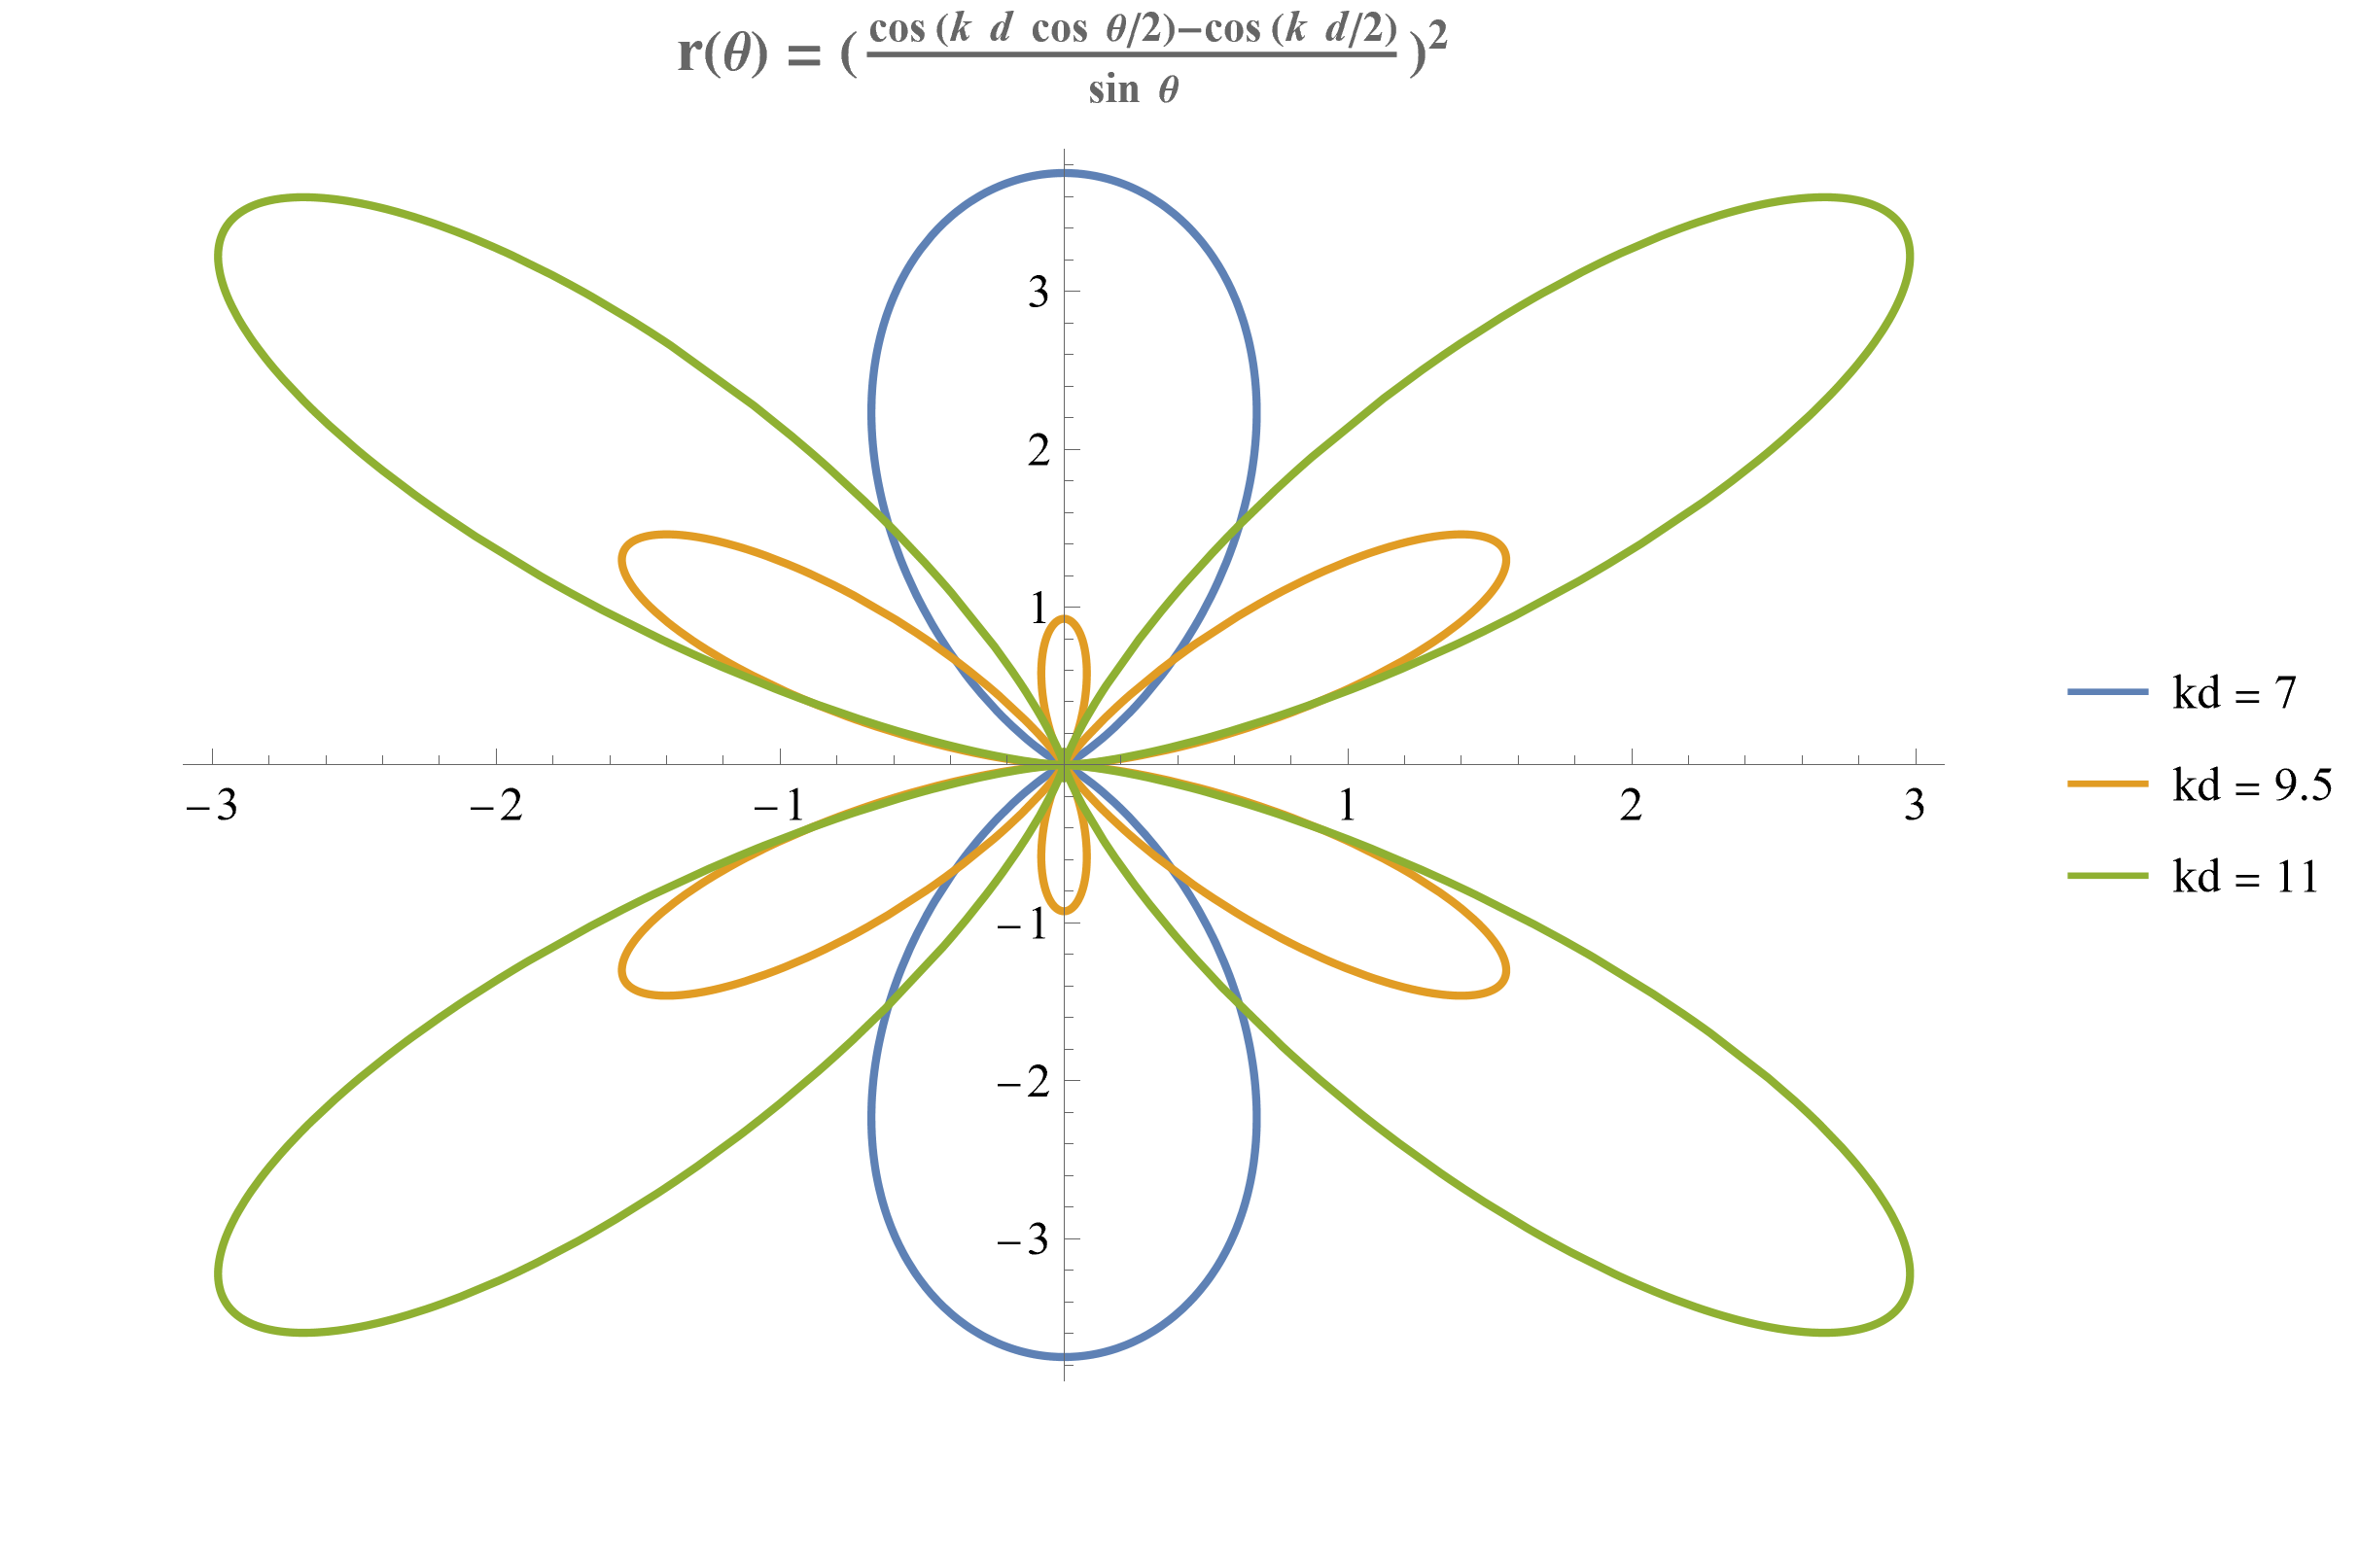
\includegraphics[width=\textwidth]{radiation_fig/energy_angular_distribution.png}
			\caption{能量角分布}
			\label{正弦天线的辐射-能量角分布}
		\end{subfigure}
		\hfill
		\begin{subfigure}[b]{0.48\textwidth}
			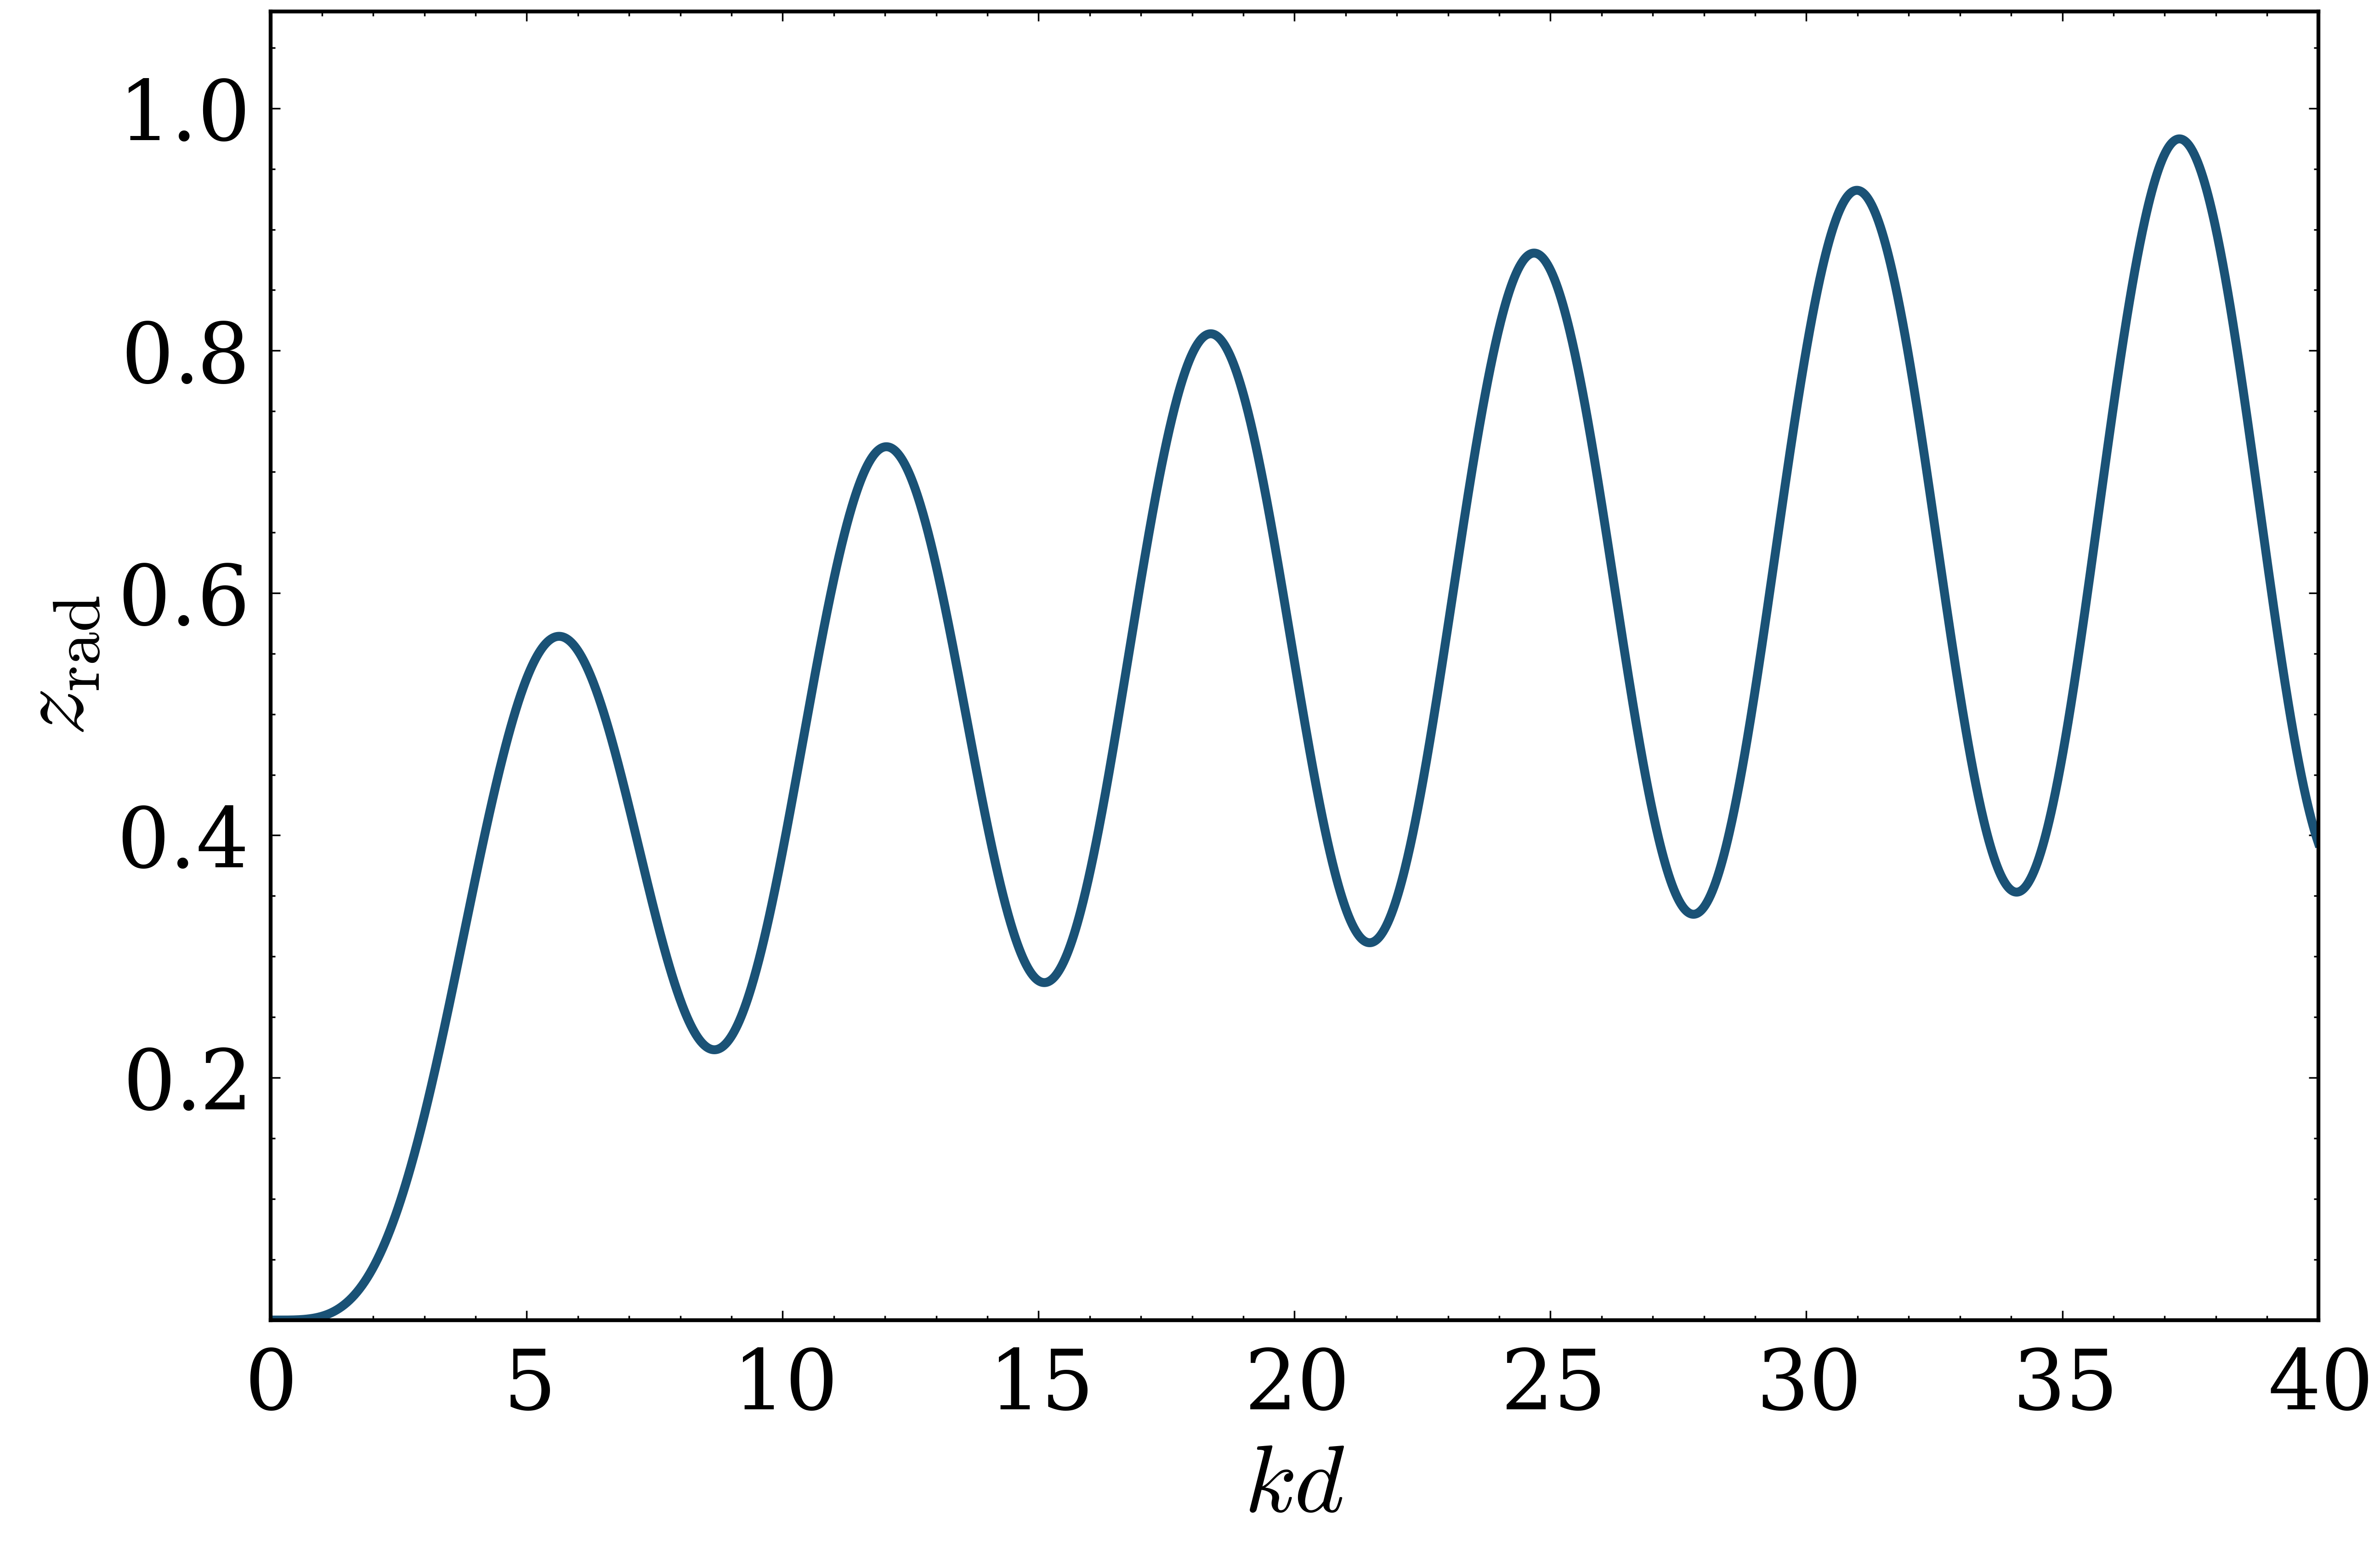
\includegraphics[width=\textwidth]{radiation_fig/relative_impedance.png}
			\caption{相对阻抗}
			\label{正弦天线的辐射-相对阻抗}
		\end{subfigure}

		\caption{正弦天线的辐射}
		\label{正弦天线的辐射}
	\end{figure}
\end{example}

\subsection{真空中的辐射场}
\subsubsection{推迟势的一般形式}
在真空中，麦克斯韦方程组简化为：
\begin{equation*}
	\nabla \cdot \vb{B} = 0,\quad
	\nabla \cdot \vb{E} = \dfrac{\rho}{\varepsilon_0},\quad
	\nabla \times \vb{B} = \mu_0 \vb{J} + \dfrac{1}{c^2} \dfrac{\partial \vb{E}}{\partial t},\quad
	\nabla \times \vb{E} = -\dfrac{\partial \vb{B}}{\partial t}.
\end{equation*}
引入标势 \(\Phi\)、矢势 \(\vb{A}\)，使得：
\begin{equation*}
	\vb{E} = -\dfrac{\partial \vb{A}}{\partial t} - \nabla \Phi, \quad \vb{B} = \nabla \times \vb{A}.
\end{equation*}
则：
\begin{align*}
	\nabla^2 \Phi - \dfrac{1}{c^2} \dfrac{\partial^2 \Phi}{\partial t^2} + \dfrac{\partial}{\partial t} \left( \nabla \cdot \vb{A} + \dfrac{1}{c^2} \dfrac{\partial \Phi}{\partial t} \right) &= -\dfrac{\rho}{\varepsilon_0}. \\
	\nabla^2 \vb{A} - \dfrac{1}{c^2} \dfrac{\partial^2 \vb{A}}{\partial t^2} - \nabla \left( \nabla \cdot \vb{A} + \dfrac{1}{c^2} \dfrac{\partial \Phi}{\partial t} \right) &= -\mu_0 \vb{J}.
\end{align*}

注意到，在变换 \(\vb{A} \to \vb{A} + \nabla \Lambda\)，\(\Phi \to \Phi - \partial \Lambda/\partial t\) 下，方程形式不变，
\(\vb{E}\)、\(\vb{B}\) 的解也不变，因此麦克斯韦方程具有一个冗余自由度，允许引入一个规范方程.

考虑到以上方程的形式，较方便的规范方程为：
\begin{equation*}
	\nabla \cdot \vb{A} + \dfrac{1}{c^2} \dfrac{\partial \Phi}{\partial t} = 0.
\end{equation*}
给出
\begin{equation*}
	\nabla^2 \Phi - \dfrac{1}{c^2} \dfrac{\partial^2 \Phi}{\partial t^2} = -\dfrac{\rho}{\varepsilon_0},\quad
	\nabla^2 \vb{A} - \dfrac{1}{c^2} \dfrac{\partial^2 \vb{A}}{\partial t^2} = -\mu_0 \vb{J}.
\end{equation*}

在该规范下，对于满足方程 \(\left( \nabla^2 - \partial^2/c^2\partial t^2 \right) \Lambda = 0\) 的解 \(\Lambda\)，形如 \(\vb{A} \to \vb{A} + \nabla \Lambda\)，\(\Phi \to \Phi - \partial\Lambda/\partial t\) 的变换不会改变电磁场的形式.

数学上易证，满足
\begin{equation*}
	\left( \nabla^2 - \dfrac{1}{c^2} \dfrac{\partial^2}{\partial t^2} \right) G(\vb{r}, t. \vb{r}', t') = -4\pi \delta(\vb{r} - \vb{r}') \delta(t - t')
\end{equation*}
的格林函数解为：
\begin{equation*}
	G^{\pm}(\vb{r}, t. \vb{r}', t') = \dfrac{1}{|\vb{r} - \vb{r}'|} \delta\left( t' - \left( t \mp \dfrac{|\vb{r} - \vb{r}'|}{c} \right) \right).
\end{equation*}
其中上符号对应推迟解，下符号对应超前解。在物理问题中，\(t\) 时刻的电磁场由该时刻以前 (\(t' < t\)) 的电荷电流分布决定，且 \(t' \to -\infty\) 时，通常无背景场.故波动方程的解为：
\begin{equation*}
	\Phi = \dfrac{1}{4\pi \varepsilon_0} \int \dfrac{\rho\left( \vb{r}', t - \dfrac{|\vb{r} - \vb{r}'|}{c} \right)}{|\vb{r} - \vb{r}'|} \d \vb{r}',\quad
	\vb{A} = \dfrac{\mu_0}{4\pi} \int \dfrac{\vb{J}\left( \vb{r}', t - \dfrac{|\vb{r} - \vb{r}'|}{c} \right)}{|\vb{r} - \vb{r}'|} \d \vb{r}'.
\end{equation*}

\subsubsection{点电荷的辐射场}
以下考虑：以轨迹 \(\vb{r}_q(\tau)\) 运动的点电荷 \(q\)，其于 \(t\) 时刻在空间中 \(\vb{r}\) 处产生的电磁场.

易知，空间中的电荷密度、电流密度为：
\begin{equation*}
	\rho\left( \vb{r}', t - \dfrac{|\vb{r} - \vb{r}'|}{c} \right) = q \,\delta\left( \vb{r}' - \vb{r}_q\left( t - \dfrac{|\vb{r} - \vb{r}'|}{c} \right) \right),\quad
	\vb{J}\left( \vb{r}', t - \dfrac{|\vb{r} - \vb{r}'|}{c} \right) = q \vb{v} \,\delta\left( \vb{r}' - \vb{r}_q\left( t - \dfrac{|\vb{r} - \vb{r}'|}{c} \right) \right).
\end{equation*}

而关于 \(\delta\) 函数的体积元与原推迟势的体积元的关系为 （其中 \(\vb{I}\) 为三维单位张量）：
\begin{align*}
	\d \left( \vb{r}' - \vb{r}_q\left( t - \dfrac{|\vb{r} - \vb{r}'|}{c} \right) \right) &= \det \left( \nabla' \left( \vb{r}' - \vb{r}_q\left( t - \dfrac{|\vb{r} - \vb{r}'|}{c} \right) \right) \right) \d \vb{r}' \\
	&= \left( 1 - \dfrac{(\vb{r} - \vb{r}') \cdot \dfrac{\d \vb{r}_q(\tau)}{\d \tau}}{c |\vb{r} - \vb{r}'|} \bigg|_{\tau = t - |\vb{r} - \vb{r}'|/c} \right) \d \vb{r}'.
\end{align*}

由于点电荷运动速度小于光速，因此 \((\vb{r}, t)\) 坐标的电磁场必定由点电荷在唯一确定的 \((\vb{r}_s, t_s)\) 坐标产生，其中，\(t_s\) 是 \(t - t_s = |\vb{r} - \vb{r}_q(t_s)|/c\) 的唯一解，\(\vb{r}_s = \vb{r}_q(t_s)\)，电荷密度、电流密度中的 \(\delta\) 函数将选择出该坐标.显然，\(\vb{r}_s\) 和 \(t_s\) 均为 \((\vb{r}, t)\) 的函数.记：
\begin{equation*}
	\vb{v} = \dfrac{\d \vb{r}_q(\tau)}{\d \tau} \bigg|_{\tau = t_s},\quad
	\vb{a} = \dfrac{\d^2\vb{r}_q(\tau)}{\d \tau^2} \bigg|_{\tau = t_s},\quad
	\vb{R} = \vb{r} - \vb{r}_s,\quad
	\kappa = 1 - \dfrac{\vb{v} \cdot \uv{R}}{c}.
\end{equation*}

进而推迟势为：
\begin{equation*}
	\Phi(\vb{r}, t) = \dfrac{q}{4\pi \varepsilon_0 \kappa R},\quad
	\vb{A}(\vb{r}, t) = \dfrac{\mu_0 q \vb{v}}{4\pi \kappa R}.
\end{equation*}

下考虑源坐标各物理量关于 \((\vb{r}, t)\) 的导数关系 （\(\uv{R}\) 是 \(\vb{R}\) 方向的单位矢量，\(R\) 是 \(\vb{R}\) 的模长）：
\begin{equation*}
	\dfrac{\partial t_s}{\partial t} = \dfrac{1}{\kappa},\quad \nabla t_s = -\dfrac{\uv{R}}{\kappa c},\quad
	\dfrac{\partial \vb{r}_s}{\partial t} = \dfrac{\vb{v}}{\kappa},\quad \nabla \vb{r}_s = -\dfrac{\uv{R} \vb{v}}{\kappa c}.
\end{equation*}
\begin{equation*}
	\dfrac{\partial \vb{v}}{\partial t} = \dfrac{\vb{a}}{\kappa}, \quad \nabla \vb{v} = -\dfrac{\uv{R} \vb{a}}{\kappa c}, \quad \nabla \times \vb{v} = -\dfrac{\uv{R} \times \vb{a}}{\kappa c},\quad
	\nabla R = \dfrac{\uv{R}}{\kappa}, \quad \dfrac{\partial R}{\partial t} = -\dfrac{\vb{v} \cdot \uv{R}}{\kappa}.
\end{equation*}
\begin{equation*}
	\nabla \uv{R} = \dfrac{1}{R} \left( \vb{I} + \dfrac{\uv{R} \vb{v}}{\kappa c} - \dfrac{\uv{R} \uv{R}}{\kappa} \right), \quad \dfrac{\partial \uv{R}}{\partial t} = \dfrac{1}{\kappa R} \left( -\vb{v} + \uv{R} (\vb{v} \cdot \uv{R}) \right).
\end{equation*}
\begin{equation*}
	\dfrac{\partial \kappa}{\partial t} = -\dfrac{1}{\kappa c R} \left( -v^2 + (\vb{v} \cdot \uv{R})^2 + R \vb{a} \cdot \uv{R} \right), \quad \nabla \kappa = -\dfrac{\vb{v}}{c R} + \dfrac{\uv{R}}{\kappa R} \left( \dfrac{\vb{v} \cdot \uv{R}}{c} - \dfrac{v^2}{c^2} + \dfrac{R}{c} \vb{a} \cdot \uv{R} \right).
\end{equation*}

进而电磁场为：
\begin{align*}
	\vb{E}(\vb{r}, t)
	&= \dfrac{q}{4\pi \varepsilon_0 \kappa^3 R^2} \bigg[ \left(1 - \dfrac{v^2}{c^2}\right) \left( \uv{R} - \dfrac{\vb{v}}{c} \right) + \dfrac{R}{c^2} \uv{R} \times \left( \left( \uv{R} - \dfrac{\vb{v}}{c} \right) \times \vb{a} \right) \bigg].\\
	\vb{B}(\vb{r}, t)
	&= \dfrac{\mu_0 q}{4\pi \kappa^3 R^2} \bigg[ \left(1 - \dfrac{v^2}{c^2}\right) \vb{v} \times \uv{R} + \dfrac{R}{c} \left( \kappa \vb{a} \times \uv{R} + \dfrac{\uv{R} \times \vb{v}}{c} \left( \vb{a} \cdot \uv{R} \right) \right) \bigg] = \dfrac{1}{c} \uv{R} \times \vb{E}.
\end{align*}

不难验证，电磁场也可写作如下形式：
\begin{align*}
	&\vb{E}(\vb{r}, t) = \dfrac{q}{4\pi \varepsilon_0} \bigg[ \dfrac{\uv{R}}{\kappa R^2} + \dfrac{1}{c} \dfrac{\partial}{\partial t} \left( \dfrac{\uv{R}}{\kappa R} \right) - \dfrac{1}{c^2} \dfrac{\partial}{\partial t} \left( \dfrac{\vb{v}}{\kappa R} \right) \bigg] = \dfrac{q}{4\pi \varepsilon_0} \bigg[ \dfrac{\uv{R}}{R^2} + \dfrac{R}{c} \dfrac{\partial}{\partial t} \left( \dfrac{\uv{R}}{R^2} \right) + \dfrac{1}{c^2} \dfrac{\partial^2 \uv{R}}{\partial t^2} \bigg].\\
	&\vb{B}(\vb{r}, t) = \dfrac{\mu_0 q}{4\pi} \bigg[ \dfrac{\vb{v} \times \uv{R}}{\kappa R^2} + \dfrac{1}{c} \dfrac{\partial}{\partial t} \left( \dfrac{\vb{v} \times \uv{R}}{\kappa R} \right) \bigg] = \dfrac{\mu_0 q}{4\pi} \bigg[ \dfrac{\vb{v} \times \uv{R}}{\kappa^2 R^2} + \dfrac{1}{c R} \dfrac{\partial}{\partial t} \left( \dfrac{\vb{v} \times \uv{R}}{\kappa} \right) \bigg].
\end{align*}

不难看到，电磁场既有按 \(R^{-2}\) 衰减的部分 (static)，也有按 \(R^{-1}\) 衰减的部分 (radiative).
后者仅当点电荷加速运动时才不为零，且只有后者的能量能传播到无穷远.

当点电荷做匀速运动时，不存在辐射电磁场，且源坐标较容易求出.

\begin{figure}[htbp]
	\centering
	\begin{subfigure}[b]{0.24\textwidth}
		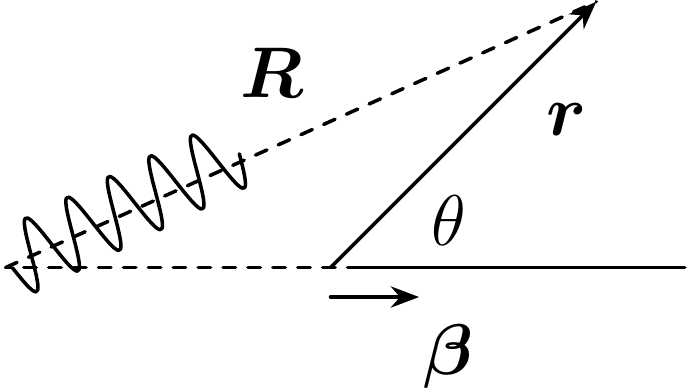
\includegraphics[width=\textwidth]{radiation_fig/charge_uniform_motion_radiation_schematic.png}
		\caption{匀速运动}
		\label{电荷运动模式示意图-匀速运动}
		\label{匀速运动电荷的辐射示意图}
	\end{subfigure}
	\hfill
	\begin{subfigure}[b]{0.28\textwidth}
		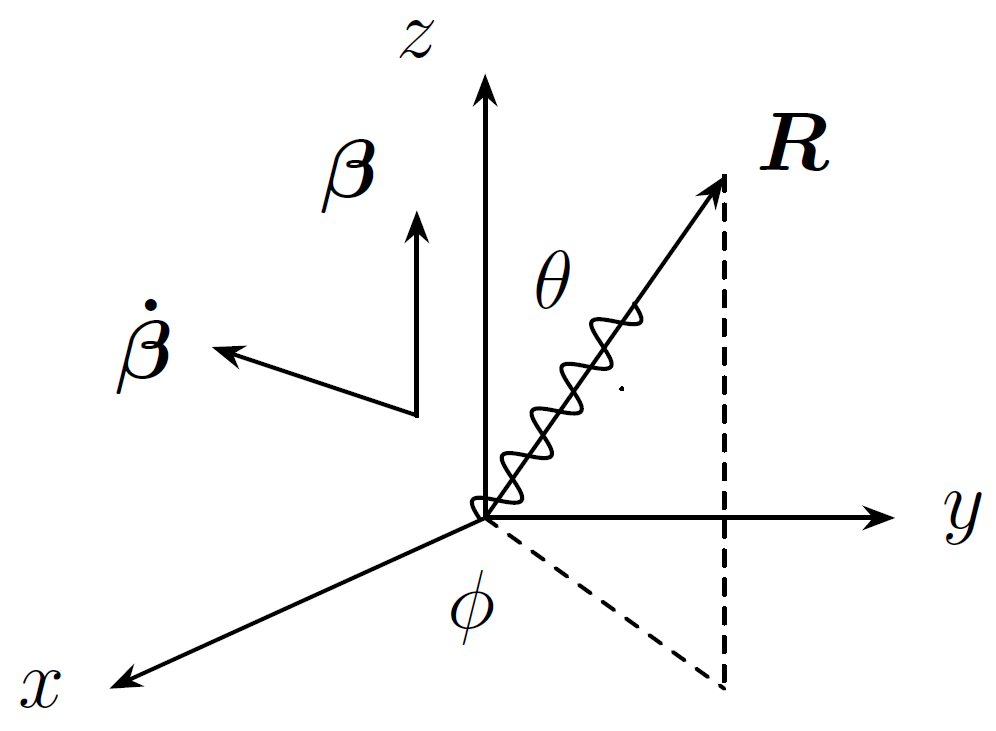
\includegraphics[width=\textwidth]{radiation_fig/charge_nonuniform_motion_radiation_schematic.png}
		\caption{非匀速运动}
		\label{电荷运动模式示意图-非匀速运动}
		\label{非匀速运动电荷的辐射示意图}
	\end{subfigure}
	\hfill
	\begin{subfigure}[b]{0.25\textwidth}
		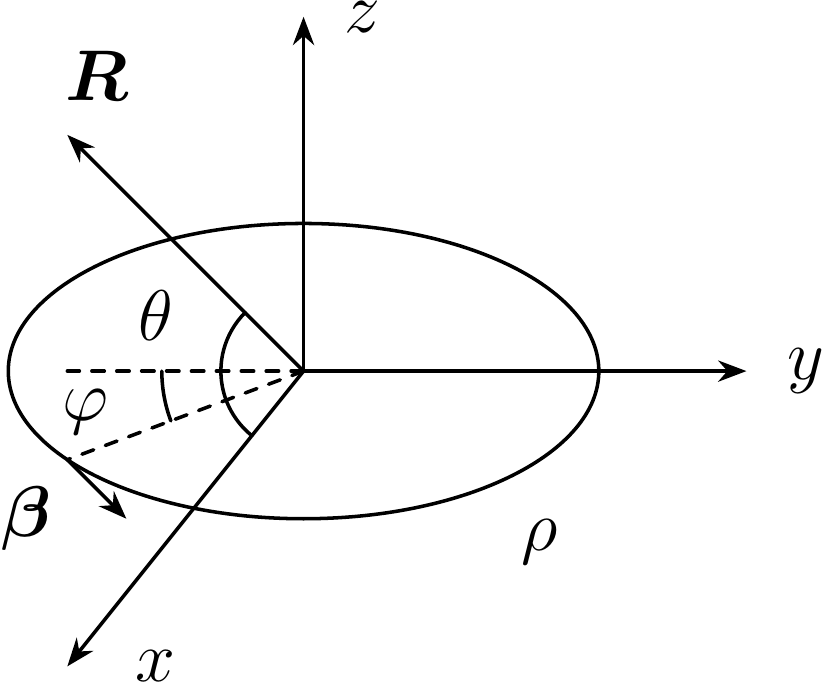
\includegraphics[width=\textwidth]{radiation_fig/charge_circular_motion_radiation_schematic.png}
		\caption{圆周运动}
		\label{电荷运动模式示意图-圆周运动}
		\label{圆周运动电荷的辐射示意图}
	\end{subfigure}
	\hfill
	\begin{subfigure}[b]{0.17\textwidth}
		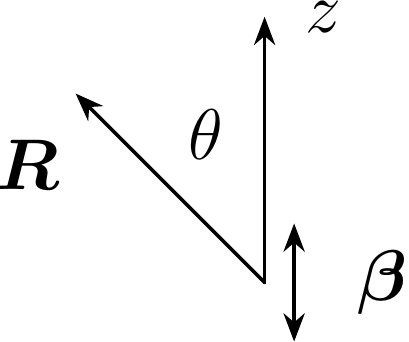
\includegraphics[width=\textwidth]{radiation_fig/charge_harmonic_motion_radiation_schematic.png}
		\caption{简谐运动}
		\label{电荷运动模式示意图-简谐运动}
		\label{简谐运动电荷的辐射示意图}
	\end{subfigure}
	\caption{电荷运动模式示意图}
	\label{电荷运动模式示意图}
\end{figure}

如图\ref{匀速运动电荷的辐射示意图}，记 \(\vb{v}\) 与 \(\vb{r}\) 的夹角为 \(\theta\)，\(|\vb{v}| = \beta c\)，则 \(\vb{R} = \vb{r} + R \vb{v}/c\)，解得：
\begin{equation*}
	R = \dfrac{r}{1 - \beta^2} \left( \beta \cos\theta + \sqrt{1 - \beta^2 \sin^2\theta} \right). \quad \kappa R = R - \dfrac{\vb{R} \cdot \vb{v}}{c} = r \sqrt{1 - \beta^2 \sin^2\theta}.
\end{equation*}
进而电磁场为：
\begin{align*}
	\vb{E}(\vb{r}, t) &= \dfrac{q}{4\pi \varepsilon_0 \kappa^3 R^2} \left(1 - \dfrac{v^2}{c^2}\right) \left( \dfrac{\vb{R}}{R} - \dfrac{\vb{v}}{c} \right) = \dfrac{q \vb{r}}{4\pi \varepsilon_0 r^3} \dfrac{1 - \beta^2}{\left(1 - \beta^2 \sin^2\theta\right)^{3/2}}.\\
	\vb{B}(\vb{r}, t) &= \dfrac{1}{c} \uv{R} \times \vb{E} = \dfrac{\mu_0 q \vb{v} \times \vb{r}}{4\pi r^3} \dfrac{1 - \beta^2}{\left(1 - \beta^2 \sin^2\theta\right)^{3/2}}.
\end{align*}

当点电荷做加速运动时，我们通常在较远的观察点关心其辐射电磁场，并忽略按 \(R^{-2}\) 衰减的部分.
\begin{equation*}
	\vb{E}(\vb{r}, t) = \dfrac{q}{4\pi \varepsilon_0 \kappa^3 c^2 R} \uv{R} \times \left( \left( \uv{R} - \dfrac{\vb{v}}{c} \right) \times \vb{a} \right),\quad
	\vb{B}(\vb{r}, t) = \dfrac{1}{c} \uv{R} \times \vb{E}.
\end{equation*}
能流密度为：
\begin{align*}
	\vb{S}(\vb{r}, t) &= \dfrac{1}{\mu_0} \vb{E} \times \vb{B} = \dfrac{q^2}{16\pi^2 \varepsilon_0 \kappa^6 c^3 R^2} \uv{R} \left| \uv{R} \times \left( \left( \uv{R} - \dfrac{\vb{v}}{c} \right) \times \vb{a} \right) \right|^2.
\end{align*}
假设点电荷在 \(\tau = \tau_1\) 到 \(\tau = \tau_2\) 的有限时间内进行了加速，则在 \(\vb{r}\) 处单位面积探测器接受到的能量为：
\begin{equation*}
	\mathcal{E}_{\text{detector}} = \int_{t = \tau_1 + |\vb{r} - \vb{r}_q(\tau_1)|/c}^{t = \tau_2 + |\vb{r} - \vb{r}_q(\tau_2)|/c} \vb{S} \cdot \uv{R} \, \d t = \int_{\tau = \tau_1}^{\tau = \tau_2} \vb{S} \cdot \uv{R} \dfrac{\d t}{\d \tau} \d \tau.
\end{equation*}
显然，更有物理意义的辐射功率密度为 \(\bm{\mathcal{P}}_{\text{rad}}(\vb{r}, t) = \vb{S} \cdot \uv{R} \d t/\d \tau\).令加速时间无穷短，得辐射功率关于源处立体角的角分布：
\begin{equation*}
	\dfrac{\d P}{\d \Omega} = R^2 \vb{S} \cdot \uv{R} \dfrac{\partial t}{\partial t_s} = \dfrac{q^2}{16\pi^2 \varepsilon_0 \kappa^5 c^3} \left| \uv{R} \times \left( \left( \uv{R} - \dfrac{\vb{v}}{c} \right) \times \vb{a} \right) \right|^2.
\end{equation*}
如图\ref{非匀速运动电荷的辐射示意图}，记 \(\uv{R}\) 与 \(\vb{v} = \vb{\beta} c\) 的夹角为 \(\theta\)（注意，\(\theta\) 不同于点电荷做匀速运动时的定义），在源处建立球坐标系，令 \(z\) 轴平行于 \(\vb{\beta}\)，适当选取零点使 \(\vb{a}\) 恰在 \(\phi = 0\) 平面内，则：
\begin{equation*}
	\vb{\beta} = \beta \left( \uv{R} \cos\theta - \uv{\theta} \sin\theta \right),\quad
	\vb{a} = \vb{a} \cdot \uv{\beta} \left( \uv{R} \cos\theta - \uv{\theta} \sin\theta \right) + |\vb{a} \times \uv{\beta}| \left( \sin\theta \cos\phi\, \uv{R} + \cos\theta \cos\phi \,\uv{\theta} - \sin\phi\, \uv{\phi} \right).
\end{equation*}
记 \(\gamma = (1 - \beta^2)^{-1/2}\)，\(\dot{\vb{\beta}} = \vb{a}/c\)，代入得辐射功率角分布：
\begin{align*}
	\dfrac{\d P}{\d \Omega} &= \dfrac{q^2}{16\pi^2 \varepsilon_0 \kappa^5 c} \left| \uv{R} \times \left( \left( \uv{R} - \vb{\beta} \right) \times \dot{\vb{\beta}} \right) \right|^2 \\
	&= \dfrac{q^2}{16\pi^2 \varepsilon_0 c (1 - \beta \cos\theta)^5} \bigg[ |\dot{\vb{\beta}}|^2 \sin^2\theta + \dfrac{|\vb{\beta} \times \dot{\vb{\beta}}|^2}{\beta^2} \left( (1 - \beta \cos\theta)^2 - \sin^2\theta \cos^2\phi (1 - \beta^2) - \sin^2\theta \right) \\
		&\qquad + 2 \left( \dot{\vb{\beta}} \cdot \uv{\beta} \right) |\dot{\vb{\beta}} \times \uv{\beta}| \sin\theta \cos\phi (\beta - \cos\theta) \bigg].
\end{align*}
积分得（记 \(\gamma = (1 - \beta^2)^{-1/2}\)，\(\dot{\vb{\beta}} = \vb{a}/c\)）：
\begin{equation*}
	P = \int \dfrac{\d P}{\d \Omega} \d \Omega = \dfrac{q^2 \gamma^6}{6\pi \varepsilon_0 c} \left( |\dot{\vb{\beta}}|^2 - |\vb{\beta} \times \dot{\vb{\beta}}|^2 \right).
\end{equation*}

最后，计算电荷辐射场频谱.

由之前的结论，以速度 \(\vb{\beta}c\)、加速度 \(\dot{\vb{\beta}}c\)、轨迹 \(\vb{r}_{q}(t_{s})\) 运动的电荷在时空坐标下产生的辐射场为
\begin{equation*}
	\vb{E}(\vb{r}, t) = \frac{q}{4\pi \varepsilon_{0} c R} \frac{\uv{R} \times \left( (\uv{R} - \vb{\beta}) \times \dot{\vb{\beta}} \right)}{(1 - \uv{R} \cdot \vb{\beta})^{3}}.
\end{equation*}
其中 \(\uv{R}\) 是电荷轨迹上的推迟点指向场点的方向矢量，满足
\begin{equation*}
	t = t_{s} + R/c, \quad R = |\vb{r} - \vb{r}_{q}(t_{s})|.
\end{equation*}

辐射场点距离远大于源点尺度，近似有 \(\uv{R}=\uv{r},\,R \approx r - \uv{R} \cdot \vb{r}_{q} \approx r\)，傅里叶变换至频率空间得
\begin{align*}
	\vb{E}(\vb{r}, \omega) &= \frac{q}{4\pi \varepsilon_{0} c r} \frac{1}{\sqrt{2\pi}} \int \frac{\uv{R} \times \left( (\uv{R} - \vb{\beta}) \times \dot{\vb{\beta}} \right)}{(1 - \uv{R} \cdot \vb{\beta})^{3}} e^{i\omega t} \, \d t \quad= \frac{q}{4\pi \varepsilon_{0} c r} \frac{1}{\sqrt{2\pi}} \int e^{i\omega (t_{s} + R/c)} \frac{\uv{R} \times \left( (\uv{R} - \vb{\beta}) \times \dot{\vb{\beta}} \right)}{(1 - \uv{R} \cdot \vb{\beta})^{2}} \, \d t_{s} \\
	&= -\frac{q e^{i\omega r/c}}{4\pi \varepsilon_{0} c r} \frac{i\omega}{\sqrt{2\pi}} \int_{-\infty}^{\infty} e^{i\omega \left( t_{s} - \uv{R} \cdot \vb{r}_{q}(t_{s})/c \right)} \uv{R} \times (\uv{R} \times \vb{\beta}) \, \d t_{s}.
\end{align*}
式中用到
\begin{equation*}
	\frac{\partial t_{s}}{\partial t} = \frac{1}{1 - \uv{R} \cdot \vb{\beta}}, \quad \frac{\partial}{\partial t_{s}} \left( \frac{\uv{R} \times (\uv{R} \times \vb{\beta})}{1 - \uv{R} \cdot \vb{\beta}} \right) = \frac{\uv{R} \times \left( (\uv{R} - \vb{\beta}) \times \dot{\vb{\beta}} \right)}{(1 - \uv{R} \cdot \vb{\beta})^{2}}.
\end{equation*}

进而辐射功率角分布频谱为
\begin{equation*}
	\frac{\d^{2} W_{\mathrm{rad}}}{\d \Omega \d \omega} = 2 r^{2} \sqrt{\frac{\varepsilon_{0}}{\mu_{0}}} | \vb{E}(\vb{r}, \omega) |^{2} = \frac{q^{2} \omega^{2}}{16\pi^{3} \varepsilon_{0} c} \left| \int_{-\infty}^{\infty} e^{i\omega \left( t_{s} - \uv{R} \cdot \vb{r}_{q}(t_{s})/c \right)} \uv{R} \times \left( \uv{R} \times \vb{\beta} \right) \, \d t_{s} \right|^{2}.
\end{equation*}

特别注意，对于周期运动，频域辐射场将呈现分立的\(\delta\)函数谱，此时只能求出单个周期内总的辐射能量，积分时应采用如下约定
\begin{equation*}
	\int_{0}^{\infty} \left( \delta(\omega - m \Omega) \right)^{2} f(m) \, \d \omega = f(\omega/\Omega) \frac{T_{\mathrm{period}}}{2\pi}.
\end{equation*}

下考虑圆周运动、简谐运动的辐射频谱.

\begin{example}
	半径为 \(a\) 的圆周运动，如图\ref{圆周运动电荷的辐射示意图}.
	\begin{equation*}
		\uv{\beta} = (\cos\varphi, \sin\varphi, 0), \quad \vb{r}_{q} = a (\sin\varphi, -\cos\varphi, 0), \quad \varphi = \frac{\beta c t_{s}}{a}.
	\end{equation*}

	取场点、偏振基矢为
	\begin{equation*}
		\uv{R} = (\cos\theta, 0, \sin\theta), \quad \uv{e}_{a} = (-\sin\theta, 0, \cos\theta), \quad \uv{e}_{b} = (0, 1, 0).
	\end{equation*}

	代入得
	\begin{align*}
		\vb{E}(\vb{r}, \omega) &= -\frac{i q \omega \beta e^{i\omega r/c}}{2\sqrt{2\pi} \varepsilon_{0} c r} \sum_{m=-\infty}^{\infty} \delta\left( \omega - m \frac{\beta c}{a} \right) \left[ -i \uv{e}_{b} J_{m}'\left( \frac{\omega a \cos\theta}{c} \right) + \uv{e}_{a} m \sin\theta \frac{J_{m}\left( \omega a \cos\theta/c \right)}{\omega a \cos\theta/c} \right]. \\
		\frac{\d^{2} W_{\mathrm{rad}}}{\d \Omega \d \omega} &= \frac{q^{2} \omega^{2} \beta^{2}}{4\pi \varepsilon_{0} c} \left( \left| \sum_{m=-\infty}^{\infty} \delta\left( \omega - m \frac{\beta c}{a} \right) J_{m}'\left( \frac{\omega a \cos\theta}{c} \right) \right|^{2} + \left| \sum_{m=-\infty}^{\infty} \delta\left( \omega - m \frac{\beta c}{a} \right) m \sin\theta \frac{J_{m}\left(\omega a \cos\theta/c \right)}{\omega a \cos\theta/c} \right|^{2} \right). \\
		\frac{\d  W_{\mathrm{rad}}}{\d \Omega} &= \int_{0}^{\infty} \frac{\d^{2} W_{\mathrm{rad}}}{\d \Omega \d \omega} \, \d \omega = \frac{q^{2} \beta^{3}}{4\pi \varepsilon_{0} a} \sum_{m=1}^{\infty} m^{2} \left[ \left( J_{m}'(m\beta \cos\theta) \right)^{2} + m^{2} \sin^{2}\theta \left( \frac{J_{m}(m\beta \cos\theta)}{m\beta \cos\theta} \right)^{2} \right] \\
		&= \frac{q^{2} \beta^{3}}{64\pi \varepsilon_{0} a} \frac{4(1 + \sin^{2}\theta) - \beta^{2} \cos^{4}\theta (1 + 3\beta^{2})}{(1 - \beta^{2} \cos^{2}\theta)^{7/2}}. \\
		W_{\mathrm{rad}} &= 2\pi \int_{-\pi/2}^{\pi/2} \frac{\d  W_{\mathrm{rad}}}{\d \Omega} \cos\theta \, \d \theta = \frac{q^{2} \gamma^{4} \beta^{3}}{3 \varepsilon_{0} a}.
	\end{align*}

	当速度接近光速 (\(\gamma \gg 1\))、观测角很小 (\(\theta \ll 1\)) 时，取连续化近似
	\begin{equation*}
		\sum_{m=-\infty}^{\infty} f(m) \delta(\omega - m \Omega) = \frac{1}{\Omega} f(\frac{\omega}{\Omega}), \quad \Omega = \beta c/a.
	\end{equation*}
	也即
	\begin{align*}
		&\sum_{m=-\infty}^{\infty} \delta\left( \omega - m \frac{\beta c}{a} \right) \left( -i \uv{e}_{b} J_{m}'\left( \frac{\omega a \cos\theta}{c} \right) + \uv{e}_{a} \sin\theta \frac{m J_{m}\left(\omega a \cos\theta/c \right)}{\omega a \cos\theta/c} \right) \\&\quad= -\frac{i a}{\sqrt{3}\pi \beta c} (\theta^{2} + \gamma^{-2}) \left( \uv{e}_{b} K_{2/3}(\xi) + i \uv{e}_{a} \frac{\theta}{\sqrt{\theta^{2} + \gamma^{-2}}} K_{1/3}(\xi) \right). \qquad
		\xi = \frac{\omega a}{3c} (\theta^{2} + \gamma^{-2})^{3/2}.
	\end{align*}
	得到
	\begin{align*}
		\frac{\d^{2} W_{\mathrm{rad}}}{\d \Omega \d \omega} &= \frac{q^{2}}{12\pi^{3} \varepsilon_{0} c} \left( \frac{\omega a}{c} \right)^{2} (\theta^{2} + \gamma^{-2})^{2} \left( (K_{2/3}(\xi))^{2} + \frac{\theta^{2}}{\theta^{2} + \gamma^{-2}} (K_{1/3}(\xi))^{2} \right). \\
		\frac{\d  W_{\mathrm{rad}}}{\d \Omega} &= \frac{7 q^{2}}{64\pi \varepsilon_{0} a (\theta^{2} + \gamma^{-2})^{5/2}} \left( 1 + \frac{5}{7} \frac{\theta^{2}}{\theta^{2} + \gamma^{-2}} \right). \\
		W_{\mathrm{rad}} &= 2\pi \int_{-\infty}^{\infty} \frac{\d  W_{\mathrm{rad}}}{\d \Omega} \, \d \theta = \frac{q^{2} \gamma^{4}}{3 \varepsilon_{0} a}.
	\end{align*}
\end{example}

\begin{example}
	幅度为\(a\)、角频率为\(\omega_{0}\) 的简谐运动，如图\ref{简谐运动电荷的辐射示意图}.
	\begin{equation*}
		\vb{r}_{q}(t) = a \cos(\omega_{0} t) \uv{z}, \quad \vb{\beta} = -\beta_{0} \sin(\omega_{0} t) \uv{z}, \quad \beta_{0} = \frac{\omega_{0} a}{c}.
	\end{equation*}

	取场点方向、偏振方向为
	\begin{equation*}
		\uv{R} = (\sin\theta, 0, \cos\theta), \quad \uv{e}_{a} = (\cos\theta, 0, -\sin\theta).
	\end{equation*}

	代入得
	\begin{align*}
		\vb{E}(\vb{r}, \omega) &= i \uv{e}_{a} \frac{q \omega \omega_{0} a e^{i\omega r/c}}{4\pi \varepsilon_{0} c^{2} r} \frac{1}{\sqrt{2\pi}} \int_{-\infty}^{\infty} e^{i\omega \left( t_{s} - a \cos(\omega_{0} t_{s}) \cos\theta/c \right)} \sin\theta \sin(\omega_{0} t_{s}) \, \d t_{s} \\
		&= -i^{1-m} \uv{e}_{a} \frac{q \omega e^{i\omega r/c}}{2\sqrt{2\pi} \varepsilon_{0} c r} \tan\theta \sum_{m=1}^{\infty} J_{m}(m\beta_{0} \cos\theta) \delta(\omega - m\omega_{0}). \\
		\frac{\d^{2} W_{\mathrm{rad}}}{\d \Omega \d \omega} &= \frac{q^{2} \omega^{2}}{4\pi \varepsilon_{0} c} \tan^{2}\theta \left| \sum_{m=1}^{\infty} J_{m}(m\beta_{0} \cos\theta) \delta(\omega - m\omega_{0}) \right|^{2}. \\
		\frac{\d  W_{\mathrm{rad}}}{\d \Omega} &= \int_{0}^{\infty} \frac{\d^{2} W_{\mathrm{rad}}}{\d \Omega \d \omega} \, \d \omega = \frac{q^{2} \omega_{0}}{4\pi \varepsilon_{0} c} \tan^{2}\theta \sum_{m=1}^{\infty} m^{2} \left( J_{m}(m\beta_{0} \cos\theta) \right)^{2} = \frac{q^{2} \omega_{0} \beta_{0}^{2} \sin^{2}\theta}{64\pi \varepsilon_{0} c} \frac{4 + \beta_{0}^{2} \cos^{2}\theta}{(1 - \beta_{0}^{2} \cos^{2}\theta)^{7/2}}. \\
		W_{\mathrm{rad}} &= 2\pi \int_{0}^{\pi} \frac{\d  W_{\mathrm{rad}}}{\d \Omega} \sin\theta \, \d \theta = \frac{q^{2} \omega_{0}^{3} a^{2}}{24 \varepsilon_{0} c^{3}} \frac{4 - 3\beta_{0}^{2}}{(1 - \beta_{0}^{2})^{3/2}}.
	\end{align*}
\end{example}
\begin{notes}
	辐射能量也可以通过如下瞬时辐射公式积分求出

	\begin{equation*}
		\frac{\d  P_{\mathrm{rad}}}{\d \Omega} = \frac{q^{2}}{16\pi^{2} \varepsilon_{0} c} \frac{| \uv{R} \times \left( (\uv{R} - \vb{\beta}) \times \dot{\vb{\beta}} \right) |^{2}}{(1 - \uv{R} \cdot \vb{\beta})^{5}}.
	\end{equation*}

	对于圆周运动
	\begin{align*}
		\uv{R} &= (\cos\theta, 0, \sin\theta), \quad
		\vb{\beta} = \beta (\cos\varphi, \sin\varphi, 0), \quad
		\dot{\vb{\beta}} = \frac{\beta^{2} c}{\rho} (-\sin\varphi, \cos\varphi, 0). \\
		\frac{\d  P_{\mathrm{rad}}}{\d \Omega} &= \frac{q^{2} \beta^{4} c}{16\pi^{2} \varepsilon_{0} \rho^{2}} \frac{1 - \sin^{2}\varphi \cos^{2}\theta + \beta^{2} \cos^{2}\theta - 2\beta \cos\varphi \cos\theta}{(1 - \beta \cos\theta \cos\varphi)^{5}}. \\
		\frac{\d  W_{\mathrm{rad}}}{\d \Omega} &= \int_{0}^{2\pi} \frac{\d  P_{\mathrm{rad}}}{\d \Omega} \frac{\rho}{\beta c} \, \d \varphi = \frac{q^{2} \beta^{3}}{64\pi \varepsilon_{0} \rho} \frac{4(1 + \sin^{2}\theta) - \beta^{2} \cos^{4}\theta (1 + 3\beta^{2})}{(1 - \beta^{2} \cos^{2}\theta)^{7/2}}.
	\end{align*}

	对于简谐运动
	\begin{align*}
		\uv{R} &= (\sin\theta, 0, \cos\theta), \quad
		\vb{\beta} = -\beta_{0} \sin(\omega_{0} t) \uv{z}, \quad
		\dot{\vb{\beta}} = -\omega_{0} \beta_{0} \cos(\omega_{0} t) \uv{z}, \quad
		\beta_{0} = \frac{\omega_{0} a}{c}. \\
		\frac{\d  P_{\mathrm{rad}}}{\d \Omega} &= \frac{q^{2} \omega_{0}^{2} \beta_{0}^{2}}{16\pi^{2} \varepsilon_{0} c} \frac{\sin^{2}\theta \cos^{2}(\omega_{0} t_{s})}{(1 + \beta_{0} \sin(\omega_{0} t_{s}) \cos\theta)^{5}}. \\
		\frac{\d  W_{\mathrm{rad}}}{\d \Omega} &= \int_{0}^{2\pi/\omega_{0}} \frac{\d  P_{\mathrm{rad}}}{\d \Omega} \, \d t_{s} = \frac{q^{2} \omega_{0} \beta_{0}^{2} \sin^{2}\theta}{64\pi \varepsilon_{0} c} \frac{4 + \beta_{0}^{2} \cos^{2}\theta}{(1 - \beta_{0}^{2} \cos^{2}\theta)^{7/2}}.
	\end{align*}

	结果与之前完全一致.

	两类运动辐射场空间分布如图\ref{点电荷周期运动辐射能量角分布},\ref{点电荷圆周运动辐射场示意图},\ref{点电荷简谐运动辐射场示意图}，轨道尺寸\(a/\lambda=1.2\)，画图截面为\(x/y/z=0\).简谐运动标注中的\(\beta\)指\(\beta_0\)，\(\eta\)指轨道相位（最大位移处\(\eta=0\)，平衡位置处\(\eta=0.25\)）.
\end{notes}

\subsubsection{局域时变电荷体系的电磁场}

本节引入双点乘、叉点乘两个张量运算符号.其中，双点乘对相邻的四个指标进行缩并，叉点乘对相邻的四个指标中的内层指标叉乘、外层指标缩并，即：
\begin{equation*}
	\uv{e}_i \uv{e}_j : \uv{e}_k \uv{e}_l = \delta_{il} \delta_{jk}, \quad
	\uv{e}_i \uv{e}_j \crossdot \uv{e}_k \uv{e}_l = \delta_{il} \epsilon_{pjk} \uv{e}_p
\end{equation*}

选取电荷体系中的不动点为原点，记电荷体系中的电荷相对原点的位矢为 \(\vb{r}'\)，观测点坐标为 \((\vb{r}, t)\)，且 \(r \gg r'\).

在大多数局域电荷体系中，对远场的电磁作用不会高于磁偶极矩、电四极矩项（更完整的讨论见下“赫兹矢量部分”），因此下仅展开到 \(\vb{r}'\) 的平方项，即：
\begin{equation*}
	|\vb{r} - \vb{r}'| \approx r \left( 1 - \frac{\uv{r} \cdot \vb{r}'}{r} + \frac{(r')^2}{2r^2} - \frac{(\uv{r} \cdot \vb{r}')^2}{2r^2} \right),
\end{equation*}
\begin{equation*}
	\frac{1}{|\vb{r} - \vb{r}'|} \approx \frac{1}{r} \left( 1 + \frac{\uv{r} \cdot \vb{r}'}{r} - \frac{(r')^2}{2r^2} + \frac{3(\uv{r} \cdot \vb{r}')^2}{2r^2} \right).
\end{equation*}

对电荷密度与电流密度也展开到对应项：
\begin{align*}
	&\rho\left( \vb{r}', t - \frac{|\vb{r} - \vb{r}'|}{c} \right) \approx \rho\left( \vb{r}', t - \frac{r}{c} \right) + \frac{\partial \rho}{c \partial t} \uv{r} \cdot \vb{r}' + \frac{1}{2} \left( \frac{\partial \rho}{c \partial t} \frac{(\uv{r} \cdot \vb{r}')^2 - (r')^2}{r} + \frac{\partial^2 \rho}{2c^2 \partial t^2} (\uv{r} \cdot \vb{r}')^2 \right),\\
	&\vb{J}\left( \vb{r}', t - \frac{|\vb{r} - \vb{r}'|}{c} \right) = \vb{J}\left( \vb{r}', t - \frac{r}{c} \right) + \frac{\partial \vb{J}}{c \partial t} \uv{r} \cdot \vb{r}'.
\end{align*}
其中由于 \(\vb{r}\) 与 \(t\) 相互独立，故：
\begin{equation*}
	\frac{\partial \rho\left( \vb{r}', t - r/c  \right)}{\partial t} = \left. \frac{\partial \rho\left( \vb{r}', t' \right)}{\partial t'} \right|_{t' = t - \frac{r}{c}}, \quad
	\nabla \rho\left( \vb{r}', t - \frac{r}{c} \right) = \left( -\frac{\uv{r}}{c} \frac{\partial \rho\left( \vb{r}', t' \right)}{\partial t'} \right) \bigg|_{t' = t - \frac{r}{c}} = -\frac{\uv{r}}{c} \frac{\partial \rho}{\partial t}.
\end{equation*}
所有关于 \(t\) 的偏导及以下将遇到的关于电荷密度的梯度皆同理.

由电荷守恒 \(\nabla' \cdot \vb{J}\left( \vb{r}', t' \right) = -\partial \rho\left( \vb{r}', t' \right)/\partial t'\)，及电荷电流分布的局域性条件（进而体系总电荷量守恒），得如下关于 \(\vb{J}\) 的积分式为：
\begin{align*}
	&\int \vb{J}\left( \vb{r}', t - \frac{r}{c} \right) \d \vb{r}' = \int \left( \nabla' \cdot (\vb{J} \vb{r}') - \vb{r}' \nabla' \cdot \vb{J}\left( \vb{r}', t - \frac{r}{c} \right) \right) \d \vb{r}' = \int \frac{\partial \rho\left( \vb{r}', t - \frac{r}{c} \right)}{\partial t} \vb{r}' \d \vb{r}'.\\
	&\int \left( \vb{r}' \vb{J}\left( \vb{r}', t - \frac{r}{c} \right) + \vb{J}\left( \vb{r}', t - \frac{r}{c} \right) \vb{r}' \right) \d \vb{r}' = \int \left( \nabla' \cdot (\vb{J} \vb{r}' \vb{r}') - \vb{r}' \vb{r}' \nabla' \cdot \vb{J}\left( \vb{r}', t - \frac{r}{c} \right) \right) \d \vb{r}' = \int \frac{\partial \rho\left( \vb{r}', t - \frac{r}{c} \right)}{\partial t} \vb{r}' \vb{r}' \d \vb{r}'.
\end{align*}

进行规范变换 \(\vb{A} \to \vb{A} + \nabla \Lambda\)，\(\Phi \to \Phi - \partial\Lambda/\partial t\)，引入规范函数：
\begin{equation*}
	\Lambda = \frac{1}{24\pi\varepsilon_0 c^2 r} \int (r')^2 \frac{\partial \rho}{\partial t} \d \vb{r}'.
\end{equation*}

不难验证 \(\left( \nabla^2 - \partial^2/c^2\partial t^2 \right) \Lambda = 0 \).经过一定运算后，得到电磁势为：
\begin{align*}
	\Phi &\stackrel{\text{GT}}{=}\frac{q}{4\pi\varepsilon_0 r} + \left( 1 + \frac{r}{c} \frac{\partial}{\partial t} \right) \frac{\uv{r} \cdot \vb{p}}{4\pi\varepsilon_0 r^2} + \left( 1 + \frac{r}{c} \frac{\partial}{\partial t} \right) \frac{\uv{r} \uv{r} : \vb{D}}{8\pi\varepsilon_0 r^3} + \frac{\uv{r} \uv{r}}{24\pi\varepsilon_0 c^2 r} : \frac{\partial^2 \vb{D}}{\partial t^2}.\\
	\vb{A}&\stackrel{\text{GT}}{=} \frac{1}{4\pi\varepsilon_0 c^2 r} \frac{\partial \vb{p}}{\partial t} + \left( 1 + \frac{r}{c} \frac{\partial}{\partial t} \right) \frac{\mu_0 \vb{m} \times \uv{r}}{4\pi r^2} + \left( 1 + \frac{r}{c} \frac{\partial}{\partial t} \right) \frac{\uv{r}}{24\pi\varepsilon_0 c^2 r^2} \cdot \frac{\partial \vb{D}}{\partial t}.
\end{align*}
其中GT(gauge transformation)指经过了规范变换，各阶矩定义为
\begin{equation*}
	q = \int \rho\left( \vb{r}', t - \frac{r}{c} \right) \d \vb{r}' = \text{const}, \quad
	\vb{p} = \int \rho\left( \vb{r}', t - \frac{r}{c} \right) \vb{r}' \d \vb{r}'.
\end{equation*}
\begin{equation*}
	\vb{D} =\int \rho\left( \vb{r}', t - \frac{r}{c} \right) \left(3\vb{r}' \vb{r}' - r'^2 \vb{I}\right) \d \vb{r}', \quad
	\vb{m} = \frac{1}{2} \int \vb{r}' \times \vb{J}\left( \vb{r}', t - \frac{r}{c} \right) \d \vb{r}'.
\end{equation*}
\(\vb{D}\) 按此定义是无迹张量，因而后面的四极辐射功率可直接使用 STF 角积分；若改用未去迹的二阶矩 \(\int\rho\,\vb{r}'\vb{r}'\,\d\vb{r}'\)，功率公式中的系数和缩并形式都必须相应重写。

进而，局域电荷体系的电磁场为：
\begin{align*}
	\vb{E}(\vb{r}, t) &= \frac{q \uv{r}}{4\pi\varepsilon_0 r^2} + \left( 1 + \frac{r}{c} \frac{\partial}{\partial t} \right) \frac{3\uv{r}(\uv{r} \cdot \vb{p}) - \vb{p}}{4\pi\varepsilon_0 r^3} + \left( 1 + \frac{r}{c} \frac{\partial}{\partial t} \right) \frac{5\uv{r}(\uv{r} \uv{r} : \vb{D}) - 2\uv{r} \cdot \vb{D}}{8\pi\varepsilon_0 r^4}
	\\
	&+ \frac{1}{4\pi\varepsilon_0 c^2 r} \left( \left( \frac{\partial^2 \vb{p}}{\partial t^2} \times \uv{r} \right) \times \uv{r} \right) - \frac{\mu_0}{4\pi r^2} \left( 1 + \frac{r}{c} \frac{\partial}{\partial t} \right) \left( \frac{\partial \vb{m}}{\partial t} \times \uv{r} \right) \\&+ \frac{1}{24\pi\varepsilon_0 c^3 r} \left[ \left( \left( \frac{\partial^3 \vb{D}}{\partial t^3} \cdot \uv{r} \right) \times \uv{r} \right) \times \uv{r} \right]
	+ \frac{1}{8\pi\varepsilon_0 c^2 r^2} \left[ 2\uv{r} \left( \uv{r} \uv{r} : \frac{\partial^2 \vb{D}}{\partial t^2} \right) - \uv{r} \cdot \frac{\partial^2 \vb{D}}{\partial t^2} \right].\\
	\vb{B}(\vb{r}, t) &= \frac{1}{4\pi\varepsilon_0 c^2 r^2} \left( 1 + \frac{r}{c} \frac{\partial}{\partial t} \right) \left( \frac{\partial \vb{p}}{\partial t} \times \uv{r} \right) + \left( 1 + \frac{r}{c} \frac{\partial}{\partial t} \right) \frac{\mu_0 \left( 3\uv{r}(\uv{r} \cdot \vb{m}) - \vb{m} \right)}{4\pi r^3}\\
	&\quad+ \frac{\mu_0}{4\pi c^2 r} \left( \left( \frac{\partial^2 \vb{m}}{\partial t^2} \times \uv{r} \right) \times \uv{r} \right) + \frac{1}{24\pi\varepsilon_0 c^4 r} \left( \left( \frac{\partial^3 \vb{D}}{\partial t^3} \cdot \uv{r} \right) \times \uv{r} \right) + \frac{1}{8\pi\varepsilon_0 c^2 r^3} \left( 1 + \frac{r}{c} \frac{\partial}{\partial t} \right) \left( \left( \frac{\partial \vb{D}}{\partial t} \cdot \uv{r} \right) \times \uv{r} \right).
\end{align*}

不难看到，\(\vb{E}\)、\(\vb{B}\) 中含有以 \(r^{-1}\) 速度衰减的部分，该部分将在无限远处给出非零的辐射能量.除静场和辐射场之外，还存在衰减速率介于两者之间的中间场项，这些项在观测距离与辐射波长量级相近时起重要作用.下文着重考虑辐射场项，将电磁场保留至与能量、角动量辐射的有关项：
\begin{align*}
	\vb{E}_{\text{rad}} &=\frac{1}{4\pi\varepsilon_0 c^2 r} \left( \left( \frac{\partial^2 \vb{p}}{\partial t^2} \times \uv{r} \right) \times \uv{r} \right) - \frac{\mu_0}{4\pi c r} \left( \frac{\partial^2 \vb{m}}{\partial t^2} \times \uv{r} \right) + \frac{1}{24\pi\varepsilon_0 c^3 r} \left[ \left( \left( \frac{\partial^3 \vb{D}}{\partial t^3} \cdot \uv{r} \right) \times \uv{r} \right) \times \uv{r} \right]\\
	&+ \frac{\partial}{\partial t} \left( \frac{3\uv{r}(\uv{r} \cdot \vb{p}) - \vb{p}}{4\pi\varepsilon_0 c r^2} \right) - \frac{\mu_0}{4\pi r^2} \left( \frac{\partial \vb{m}}{\partial t} \times \uv{r} \right) + \frac{1}{8\pi\varepsilon_0 c^2 r^2} \left[ 2\uv{r} \left( \uv{r} \uv{r} : \frac{\partial^2 \vb{D}}{\partial t^2} \right) - \uv{r} \cdot \frac{\partial^2 \vb{D}}{\partial t^2} \right].\\
	\vb{B}_{\text{rad}}&=\frac{1}{4\pi\varepsilon_0 c^3 r} \left( \frac{\partial^2 \vb{p}}{\partial t^2} \times \uv{r} \right) + \frac{\mu_0}{4\pi c^2 r} \left( \left( \frac{\partial^2 \vb{m}}{\partial t^2} \times \uv{r} \right) \times \uv{r} \right) + \frac{1}{24\pi\varepsilon_0 c^4 r} \left( \left( \frac{\partial^3 \vb{D}}{\partial t^3} \cdot \uv{r} \right) \times \uv{r} \right)\\
	&+ \frac{1}{4\pi\varepsilon_0 c^2 r^2} \left( \frac{\partial \vb{p}}{\partial t} \times \uv{r} \right) + \frac{\partial}{\partial t} \left( \frac{\mu_0 \left( 3\uv{r}(\uv{r} \cdot \vb{m}) - \vb{m} \right)}{4\pi c r^2} \right) + \frac{1}{8\pi\varepsilon_0 c^3 r^2} \left( \left( \frac{\partial^2 \vb{D}}{\partial t^2} \cdot \uv{r} \right) \times \uv{r} \right).
\end{align*}

进而，能量辐射功率为：
\begin{align*}
	\frac{\d P_{\text{rad}}}{\d \Omega} & = \left. \frac{r^2}{\mu_0} \text{Re}\left[ \vb{E}_{\text{rad}} \times \vb{B}_{\text{rad}}^* \right] \cdot \uv{r} \right|_{r \to \infty}                                                                                                                                                                                 \\&= \frac{1}{16\pi^2\varepsilon_0 c^3} \left| \frac{\partial^2 \vb{p}}{\partial t^2} \times \uv{r} \right|^2 + \frac{1}{16\pi^2\varepsilon_0 c^5} \left| \frac{\partial^2 \vb{m}}{\partial t^2} \times \uv{r} \right|^2
	+ \frac{1}{576\pi^2\varepsilon_0 c^5} \left| \left( \frac{\partial^3 \vb{D}}{\partial t^3} \cdot \uv{r} \right) \times \uv{r} \right|^2 + \text{ct}.                                                                                                                                                                                                          \\
	P_{\text{rad}}                      & = \frac{1}{6\pi\varepsilon_0 c^3} \left| \frac{\partial^2 \vb{p}}{\partial t^2} \right|^2 + \frac{1}{6\pi\varepsilon_0 c^5} \left| \frac{\partial^2 \vb{m}}{\partial t^2} \right|^2 + \frac{1}{720\pi\varepsilon_0 c^5} \left( \frac{\partial^3 \vb{D}}{\partial t^3} : \frac{\partial^3 \vb{D}}{\partial t^3} \right).
\end{align*}
四极项的系数来自无迹条件下的角积分
\begin{equation*}
	\int \left|(\vb{Q}\cdot\uv{r})\times\uv{r}\right|^2 \d\Omega
	=\frac{4\pi}{5}\,\vb{Q}:\vb{Q},\qquad \Tr \vb{Q}=0,
\end{equation*}
代入上式的微分功率系数 \(1/(576\pi^2\varepsilon_0 c^5)\) 即给出 \(1/(720\pi\varepsilon_0 c^5)\)。

角动量辐射功率为
\begin{align*}
	&\frac{\d^2 \vb{L}_{\text{rad}}}{\d t \, \d \Omega} = \left. r^2 \uv{r} \cdot \left( \vb{T}_{\text{em}} \times \vb{r} \right) \right|_{r \to \infty}
	=\left. \varepsilon_0 r^3 \left(
	\left( \vb{E} \cdot \uv{r} \right) \left( \vb{E} \times \uv{r} \right) +
	c^2 \left( \vb{B} \cdot \uv{r} \right) \left( \vb{B} \times \uv{r} \right)
	\right) \right|_{r \to \infty}
	\\
	&\,= \frac{1}{8\pi\varepsilon_0 c^3} \left( \uv{r} \cdot \frac{\partial \vb{p}}{\partial t} \right) \left( \uv{r} \times \frac{\partial^2 \vb{p}}{\partial t^2} \right) + \frac{1}{8\pi\varepsilon_0 c^5} \left( \uv{r} \cdot \frac{\partial \vb{m}}{\partial t} \right) \left( \uv{r} \times \frac{\partial^2 \vb{m}}{\partial t^2} \right)+ \frac{1}{192\pi\varepsilon_0 c^5} \left( \uv{r} \uv{r} : \frac{\partial^2 \vb{D}}{\partial t^2} \right) \left( \uv{r} \times \left( \frac{\partial^3 \vb{D}}{\partial t^3} \cdot \uv{r} \right) \right) +\text{ct}.\\
	&\frac{\d  \vb{L}_{\text{rad}}}{\d t} = \frac{1}{6\pi\varepsilon_0 c^3} \left( \frac{\partial \vb{p}}{\partial t} \times \frac{\partial^2 \vb{p}}{\partial t^2} \right) + \frac{1}{6\pi\varepsilon_0 c^5} \left( \frac{\partial \vb{m}}{\partial t} \times \frac{\partial^2 \vb{m}}{\partial t^2} \right) + \frac{1}{360\pi\varepsilon_0 c^5} \left( \frac{\partial^2 \vb{D}}{\partial t^2} \cdot \left( \frac{\partial^3 \vb{D}}{\partial t^3} \right) \right).
\end{align*}
其中，来源于不同阶多极矩耦合的交叉项（ct,cross-terms）关于立体角积分后得零.\(\vb{T}_{\text{em}}\) 为电磁场应力张量：
\begin{equation*}
	\vb{T}_{\text{em}} = \varepsilon_0 \left( \vb{E}\vb{E} + c^2 \vb{B}\vb{B} - \frac{1}{2} \left( E^2 + c^2 B^2 \right) \vb{I} \right).
\end{equation*}

\textbf{考虑以下辐射问题算例}：两个点电荷在库仑力下的二体运动，忽略万有引力，忽略动力学上的相对论效应，则两者做经典开普勒型运动，下分为异号双曲线轨道、异号椭圆轨道、同号双曲线轨道讨论运动中的电磁辐射.


\begin{example}
	异号双曲线轨道

	记两电荷带电量为 \(q_1, -q_2\)（\(q_1 q_2 > 0\)），质量为 \(M_1, M_2\)，由2指向1的位矢为 \(\vb{r}\)，记
	\begin{equation*}
		\alpha = \frac{q_1 q_2}{4\pi\varepsilon_0}, \quad \mu = \frac{M_1 M_2}{M_1 + M_2}, \quad \Gamma = \frac{q_1}{M_1} + \frac{q_2}{M_2}.
	\end{equation*}

	则二体运动方程、二体角动量、质心系中体系的电偶极矩为
	\begin{equation*}
		\mu \frac{\d^2\vb{r}}{\d t^2} = -\frac{\alpha}{r^3}\vb{r}, \quad \vb{L} = \mu \vb{r} \times \frac{\d \vb{r}}{\d t}, \quad \vb{p} = \Gamma \mu \vb{r}.
	\end{equation*}

	进而
	\begin{align*}
		\frac{\d \vb{p}}{\d t} &= \Gamma \mu \frac{\d \vb{r}}{\d t}, \quad \frac{\d^2\vb{p}}{\d t^2} = -\frac{\Gamma \alpha}{r^3}\vb{r}, \quad
		\left( \frac{\d \vb{p}}{\d t} \right) \times \left( \frac{\d^2\vb{p}}{\d t^2} \right) = \frac{\Gamma^2 \alpha \vb{L}}{r^3}, \quad \left| \frac{\d^2\vb{p}}{\d t^2} \right|^2 = \frac{\Gamma^2 \alpha^2}{r^4}.
	\end{align*}

	运用开普勒运动的结论
	\begin{equation*}
		r = \frac{p}{1 + e\cos\theta}, \quad \frac{\d t}{\d \theta} = \sqrt{\frac{\mu p^3}{\alpha}} \frac{1}{(1 + e\cos\theta)^2}, \quad L = \sqrt{\mu\alpha p}.
	\end{equation*}

	进而运动过程中损失的能量、角动量为
	\begin{align*}
		E_{\text{loss}} &= \frac{1}{6\pi\varepsilon_0 c^3} \int \left| \frac{\d^2\vb{p}}{\d t^2} \right|^2 \d t = \frac{\Gamma^2 \alpha^2}{6\pi\varepsilon_0 c^3} \int_{-\pi + \arccos(1/e)}^{\pi - \arccos(1/e)} \frac{1}{r^4} \frac{\d t}{\d \theta} \d \theta \\
		&= \frac{\Gamma^2 \alpha^{3/2} \mu^{1/2}}{6\pi\varepsilon_0 c^3 p^{5/2}} \left[ 3\sqrt{e^2 - 1} + (2 + e^2)\left( \pi - \arccos\left( \frac{1}{e} \right) \right) \right], \\
		\vb{L}_{\text{loss}} &= \frac{1}{6\pi\varepsilon_0 c^3} \int\left( \frac{\d \vb{p}}{\d t} \right) \times \left( \frac{\d^2\vb{p}}{\d t^2} \right) \d t= \frac{\Gamma^2 \alpha \vb{L}}{6\pi\varepsilon_0 c^3} \int_{-\pi + \arccos(1/e)}^{\pi - \arccos(1/e)} \frac{1}{r^3} \frac{\d t}{\d \theta} \d \theta \\
		&= \frac{\Gamma^2 \mu \alpha \uv{L}}{3\pi\varepsilon_0 c^3 p} \left( \sqrt{e^2 - 1} + \pi - \arccos\left( \frac{1}{e} \right) \right).
	\end{align*}
\end{example}

\begin{example}
	异号椭圆轨道

	以下一切符号规定同异号双曲线轨道.由于观测时，我们更关心周期性椭圆运动的平均效应，因此下考虑周期平均后的辐射损失能量、角动量.
	\begin{align*}
		-\frac{\d E}{\d t} &= \frac{\Gamma^2 \alpha^2}{6\pi\varepsilon_0 c^3 T} \int_{0}^{2\pi} \frac{1}{r^4} \frac{\d t}{\d \theta} \d \theta = \frac{\Gamma^2 \alpha^2}{6\pi\varepsilon_0 c^3 p^4} \left(1 + \frac{e^2}{2}\right) (1 - e^2)^{3/2}, \\
		-\frac{\d \vb{L}}{\d t} &= \frac{\Gamma^2 \alpha \vb{L}}{6\pi\varepsilon_0 c^3 T} \int_{0}^{2\pi} \frac{1}{r^3} \frac{\d t}{\d \theta} \d \theta = \frac{\Gamma^2 \alpha^{3/2} \mu^{1/2}}{6\pi\varepsilon_0 c^3 p^{5/2}} (1 - e^2)^{3/2} \uv{L}.
	\end{align*}
	其中
	\begin{equation*}
		r = \frac{p}{1 + e\cos\theta}, \quad \frac{\d t}{\d \theta} = \sqrt{\frac{\mu p^3}{\alpha}} \frac{1}{(1 + e\cos\theta)^2}, \quad L = \sqrt{\mu\alpha p}, \quad T = \frac{2\pi}{(1 - e^2)^{3/2}} \sqrt{\frac{\mu p^3}{\alpha}}.
	\end{equation*}

	可见两电荷将做准焦距、离心率不断减小的椭圆轨道运动.具体而言，由
	\begin{equation*}
		L = \sqrt{\mu\alpha p}, \quad \frac{\d L}{\d t} = \frac{1}{2}\sqrt{\frac{\alpha\mu}{p}} \frac{\d p}{\d t}, \quad E = -\frac{\alpha(1 - e^2)}{2p}, \quad \frac{\d E}{\d t} = \frac{\alpha}{2p^2}\left[(1 - e^2)\frac{\d p}{\d t} + 2ep\frac{\d e}{\d t}\right]
	\end{equation*}

	得
	\begin{equation*}
		\frac{\d e}{e \d t} = \frac{3}{4}\frac{\d p}{p \d t} = -\frac{(1 - e^2)^{3/2} \alpha \Gamma^2}{4\pi\varepsilon_0 c^3 p^3}.
	\end{equation*}

	记 \(p(t=0) = p_i\)，\(e(t=0) = e_i\)，\(\tau = \frac{\pi\varepsilon_0 c^3 p_i^3}{\alpha \Gamma^2}\)，解得椭圆轨道参数随时间的变化规律为
	\begin{equation*}
		\left(\frac{p}{p_i}\right)^{3/2} = \left(\frac{e}{e_i}\right)^2 = \frac{1}{e_i^2}\left\{1 - \frac{1}{4}\left[\sqrt{1 - e_i^2} + \frac{1}{\sqrt{1 - e_i^2}} - e_i^4 \frac{t}{4\tau} - \sqrt{\left(\sqrt{1 - e_i^2} + \frac{1}{\sqrt{1 - e_i^2}} - e_i^4 \frac{t}{4\tau}\right)^2 - 4}\right]^2\right\}.
	\end{equation*}

	进而，两点电荷相互坠落并最终相撞的时刻为
	\begin{equation*}
		t\big|_{p=0} = \left(\frac{(1 - e_i^2)^{-1/4} - (1 - e_i^2)^{1/4}}{e_i^2}\right)^2 4\tau.
	\end{equation*}

	特别地，对于圆轨道，\(e_i = 0\)，对上式取极限得
	\begin{equation*}
		e(t) = 0, \quad p(t) = p_i \left(1 - \frac{t}{\tau}\right)^{1/3}, \quad t\big|_{p=0} = \tau.
	\end{equation*}

	当然，由于 \(p\) 很小时点电荷速度显然较大，动力学的相对论效应不可忽略，因此最后对相撞时刻的求解只是一种估算.
\end{example}

\begin{example}
	同号双曲线轨道

	记两电荷带电量为 \(q_1, q_2\)（\(q_1 q_2 > 0\)），质量为 \(M_1, M_2\)，由2指向1的位矢为 \(\vb{r}\)，记
	\begin{equation*}
		\alpha = \frac{q_1 q_2}{4\pi\varepsilon_0}, \quad \mu = \frac{M_1 M_2}{M_1 + M_2}, \quad \Gamma = \frac{q_1}{M_1} - \frac{q_2}{M_2}.
	\end{equation*}

	则二体运动方程、二体角动量、质心系中体系的电偶极矩、磁矩、电四极矩为
	\begin{align*}
		\mu \frac{\d^2\vb{r}}{\d t^2} &= -\frac{\alpha}{r^3}\vb{r}, \quad \vb{L} = \mu \vb{r} \times \frac{\d \vb{r}}{\d t}, \quad \vb{p} = \Gamma \mu \vb{r}, \quad
		\vb{m} = \frac{q_1 M_2^2 + q_2 M_1^2}{M_1 M_2 (M_1 + M_2)} \vb{L}, \quad \vb{D} = \frac{q_1 M_2^2 + q_2 M_1^2}{(M_1 + M_2)^2} \left(3\vb{r}\vb{r} - r^2 \vb{I}\right).
	\end{align*}

	不难看到，当两电荷的荷质比相等时，\(\Gamma = 0\)，不存在电偶极矩辐射，同时由于 \(\vb{L}\) 的零级解守恒，故最低阶为电四极矩辐射，应当分类讨论.


	a.若 \(\Gamma \neq 0\)，最低阶为电偶极矩辐射
	\begin{align*}
		\frac{\d \vb{p}}{\d t} &= \Gamma \mu \frac{\d \vb{r}}{\d t}, \quad \frac{\d^2\vb{p}}{\d t^2} = \frac{\Gamma \alpha}{r^3}\vb{r}, \quad
		\left(\frac{\d \vb{p}}{\d t}\right) \times \left(\frac{\d^2\vb{p}}{\d t^2}\right) = -\frac{\Gamma^2 \alpha \vb{L}}{r^3}, \quad \left| \frac{\d^2\vb{p}}{\d t^2} \right|^2 = \frac{\Gamma^2 \alpha^2}{r^4}.
	\end{align*}

	运用开普勒运动的结论
	\begin{equation*}
		r = \frac{p}{e\cos\theta - 1}, \quad \frac{\d t}{\d \theta} = \sqrt{\frac{\mu p^3}{\alpha}} \frac{1}{(e\cos\theta - 1)^2}, \quad L = \sqrt{\mu\alpha p}.
	\end{equation*}

	进而运动过程中损失的能量、角动量为
	\begin{align*}
		E_{\text{loss}} &= \frac{1}{6\pi\varepsilon_0 c^3} \int \left| \frac{\d^2\vb{p}}{\d t^2} \right|^2 \d t = \frac{\Gamma^2 \alpha^2}{6\pi\varepsilon_0 c^3} \int_{-\arccos(1/e)}^{\arccos(1/e)} \frac{1}{r^4} \frac{\d t}{\d \theta} \d \theta \\
		&= \frac{\Gamma^2 \alpha^{3/2} \mu^{1/2}}{6\pi\varepsilon_0 c^3 p^{5/2}} \left[ -3\sqrt{e^2 - 1} + (2 + e^2)\arccos\left(\frac{1}{e}\right) \right], \\
		\vb{L}_{\text{loss}} &= \frac{1}{6\pi\varepsilon_0 c^3} \int\left(\frac{\d \vb{p}}{\d t}\right) \times \left(\frac{\d^2\vb{p}}{\d t^2}\right) \d t = \frac{\Gamma^2 \alpha \vb{L}}{6\pi\varepsilon_0 c^3} \int_{-\arccos(1/e)}^{\arccos(1/e)} \frac{1}{r^3} \frac{\d t}{\d \theta} \d \theta \\
		&= -\frac{\Gamma^2 \mu \alpha \uv{L}}{3\pi\varepsilon_0 c^3 p} \left( \sqrt{e^2 - 1} - \arccos\left(\frac{1}{e}\right) \right).
	\end{align*}

	记入射半径为 \(b\)，入射相对速度为 \(v_0\)，则
	\begin{equation*}
		E = \frac{1}{2}\mu v_0^2, \quad L = \mu v_0 b, \quad p = \frac{L^2}{\mu\alpha} = \frac{\mu v_0^2 b^2}{\alpha}, \quad e = \sqrt{1 + \frac{2 E L^2}{\alpha^2 \mu}} = \sqrt{1 + \left( \frac{\mu v_0^2 b}{\alpha} \right)^2}.
	\end{equation*}

	代入得
	\begin{align*}
		E_{\text{loss}} &= \frac{\Gamma^2 \alpha^4}{6\pi\varepsilon_0 c^3 \mu^2 v_0^5 b^5} \left[ -3\frac{\mu v_0^2 b}{\alpha} + \left( 3 + \left( \frac{\mu v_0^2 b}{\alpha} \right)^2 \right) \arctan\left( \frac{\mu v_0^2 b}{\alpha} \right) \right], \\
		\vb{L}_{\text{loss}} &= -\frac{\Gamma^2 \mu \alpha \uv{L}}{3\pi\varepsilon_0 c^3 p} \left( \frac{\mu v_0^2 b}{\alpha} - \arctan\left( \frac{\mu v_0^2 b}{\alpha} \right) \right).
	\end{align*}

	对于较小的入射半径
	\begin{equation*}
		E_{\text{loss}}\big|_{b \to 0} = \frac{2\Gamma^2 \mu^3 v_0^5}{45\pi\varepsilon_0 c^3 \alpha}, \quad \vb{L}_{\text{loss}}\big|_{b \to 0} = -\frac{\Gamma^2 \mu^3 v_0^4 b \uv{L}}{9\pi\varepsilon_0 c^3 \alpha} \to 0.
	\end{equation*}


	b.若 \(\Gamma = 0\)，最低阶为电四极矩辐射
	记 \(\chi = q_1/M_1=q_2/M_2\)，则 \(\vb{D} = \chi \mu \left( 3\vb{r}\vb{r} - r^2 \vb{I} \right)\)，其各阶变化率为
	\begin{align*}
		\frac{\d \vb{D}}{\d t} &= \chi \mu \left( 3\frac{\d \vb{r}}{\d t}\vb{r} + 3\vb{r}\frac{\d \vb{r}}{\d t} - 2\left( \vb{r} \cdot \frac{\d \vb{r}}{\d t} \right)\vb{I} \right), \\
		\frac{\d^2\vb{D}}{\d t^2} &= 2\chi \alpha p \left( \frac{3\vb{r}\vb{r} - r^2 \vb{I}}{r^3 p} + \frac{\mu^2}{L^2} \left( 3\frac{\d \vb{r}}{\d t}\frac{\d \vb{r}}{\d t} - \left| \frac{\d \vb{r}}{\d t} \right|^2 \vb{I} \right) \right), \\
		\frac{\d^3\vb{D}}{\d t^3} &= -\frac{2\chi \alpha}{r^3} \left( 9\frac{\vb{r}\vb{r}}{r^2} \left( \vb{r} \cdot \frac{\d \vb{r}}{\d t} \right) - 6\left( \frac{\d \vb{r}}{\d t}\vb{r} + 3\vb{r}\frac{\d \vb{r}}{\d t} \right) + \left( \vb{r} \cdot \frac{\d \vb{r}}{\d t} \right)\vb{I} \right).\\
		\frac{\d^3\vb{D}}{\d t^3} : \frac{\d^3\vb{D}}{\d t^3} &= \frac{24\chi^2 \alpha^2}{r^6} \left( -11\left( \vb{r} \cdot \frac{\d \vb{r}}{\d t} \right)^2 + 12 r^2 \left| \frac{\d \vb{r}}{\d t} \right|^2 \right).\\
		\frac{\d^2\vb{D}}{\d t^2} \cdot \left( \frac{\d^3\vb{D}}{\d t^3} \right) &= \frac{36\chi^2 \alpha^2 p \vb{L}}{\mu r^5} \left( \frac{2r}{p} + \frac{3\mu^2}{L^2} \left( \vb{r} \cdot \frac{\d \vb{r}}{\d t} \right)^2 - \frac{2\mu^2}{L^2} r^2 \left| \frac{\d \vb{r}}{\d t} \right|^2 \right).
	\end{align*}

	运用开普勒运动的结论
	\begin{equation*}
		r = \frac{p}{e\cos\theta - 1}, \quad \frac{\d \vb{r}}{\d t} = \frac{L}{\mu r} \left( \frac{e\sin\theta}{e\cos\theta - 1}\uv{r} + \uv{\theta} \right), \quad \frac{\d t}{\d \theta} = \sqrt{\frac{\mu p^3}{\alpha}} \frac{1}{(e\cos\theta - 1)^2}, \quad L = \sqrt{\mu\alpha p}.
	\end{equation*}

	经过繁琐的积分得
	\begin{align*}
		E_{\text{loss}} &= \int_{-\arccos(1/e)}^{\arccos(1/e)} \frac{1}{720\pi\varepsilon_0 c^5} \left( \frac{\partial^3\vb{D}}{\partial t^3} : \frac{\partial^3\vb{D}}{\partial t^3} \right) \frac{\d t}{\d \theta} \d \theta \\
		&= \frac{4\chi^2 \alpha^{5/2}}{5\pi\varepsilon_0 c^5 \mu^{1/2} p^{7/2}} \left[ \left( 1 + \frac{73}{24}e^2 + \frac{37}{96}e^4 \right)\arccos\left(\frac{1}{e}\right) - \sqrt{e^2 - 1} \frac{602 + 673e^2}{288} \right], \\
		\vb{L}_{\text{loss}} &= \int_{-\arccos(1/e)}^{\arccos(1/e)} \frac{1}{360\pi\varepsilon_0 c^5} \left( \frac{\partial^2\vb{D}}{\partial t^2} \cdot \left( \frac{\partial^3\vb{D}}{\partial t^3} \right) \right) \frac{\d t}{\d \theta} \d \theta \\
		&= \frac{4\chi^2 \alpha^2 \uv{L}}{5\pi\varepsilon_0 c^5 p^2} \left[ \left( 1 + \frac{7}{8}e^2 \right)\arccos\left(\frac{1}{e}\right) - \sqrt{e^2 - 1} \frac{13 + 2e^2}{8} \right].
	\end{align*}
\end{example}
\begin{notes}
	与广义相对论的联系：在广义相对论中，引力波最低阶能量、角动量辐射功率由质量四极矩贡献.考虑做二体椭圆运动的质量为 \(M_1\) 和 \(M_2\) 的质点，记
	\begin{equation*}
		\alpha = G M_1 M_2, \quad \mu = \frac{M_1 M_2}{M_1 + M_2}.
	\end{equation*}

	设2指向1的位矢为 \(\vb{r}\)，则二体运动方程、二体角动量、质心系中体系的质量四极矩为
	\begin{equation*}
		\mu \frac{\d^2\vb{r}}{\d t^2} = -\frac{\alpha}{r^3}\vb{r}, \quad \vb{L} = \mu \vb{r} \times \frac{\d \vb{r}}{\d t}, \quad \vb{Q} = \mu \left( 3\vb{r}\vb{r} - r^2 \vb{I} \right).
	\end{equation*}

	进而，质量四极矩的各阶变化率为
	\begin{align*}
		\frac{\d \vb{Q}}{\d t} &= \mu \left( 3\frac{\d \vb{r}}{\d t}\vb{r} + 3\vb{r}\frac{\d \vb{r}}{\d t} - 2\left( \vb{r} \cdot \frac{\d \vb{r}}{\d t} \right)\vb{I} \right), \\
		\frac{\d^2\vb{Q}}{\d t^2} &= 2\alpha p \left( -\frac{3\vb{r}\vb{r} - r^2 \vb{I}}{r^3 p} + \frac{\mu^2}{L^2} \left( 3\frac{\d \vb{r}}{\d t}\frac{\d \vb{r}}{\d t} - \left| \frac{\d \vb{r}}{\d t} \right|^2 \vb{I} \right) \right), \\
		\frac{\d^3\vb{Q}}{\d t^3} &= \frac{2\alpha}{r^3} \left( 9\frac{\vb{r}\vb{r}}{r^2} \left( \vb{r} \cdot \frac{\d \vb{r}}{\d t} \right) - 6\left( \frac{\d \vb{r}}{\d t}\vb{r} + 3\vb{r}\frac{\d \vb{r}}{\d t} \right) + \left( \vb{r} \cdot \frac{\d \vb{r}}{\d t} \right)\vb{I} \right).\\
		\frac{\d^3\vb{Q}}{\d t^3} : \frac{\d^3\vb{Q}}{\d t^3} &= \frac{24\alpha^2}{r^6} \left( -11\left( \vb{r} \cdot \frac{\d \vb{r}}{\d t} \right)^2 + 12 r^2 \left| \frac{\d \vb{r}}{\d t} \right|^2 \right).\\
		\frac{\d^2\vb{Q}}{\d t^2} \crossdot \left( \frac{\d^3\vb{Q}}{\d t^3} \right) &= \frac{36\alpha^2 p \vb{L}}{\mu r^5} \left( \frac{2r}{p} - \frac{3\mu^2}{L^2} \left( \vb{r} \cdot \frac{\d \vb{r}}{\d t} \right)^2 + \frac{2\mu^2}{L^2} r^2 \left| \frac{\d \vb{r}}{\d t} \right|^2 \right).
	\end{align*}

	由于观测时更关心周期性椭圆运动的平均效应，因此考虑周期平均后的辐射损失能量、角动量.运用开普勒运动的结论
	\begin{equation*}
		r = \frac{p}{1 + e\cos\theta}, \quad \frac{\d \vb{r}}{\d t} = \frac{L}{\mu r} \left( \frac{e\sin\theta}{1 + e\cos\theta}\uv{r} + \uv{\theta} \right), \quad L = \sqrt{\mu\alpha p}, \quad T = \frac{2\pi}{(1 - e^2)^{3/2}} \sqrt{\frac{p^3}{\alpha\mu}}.
	\end{equation*}

	并带入
	\begin{equation*}
		\frac{\d t}{\d \theta} = \sqrt{\frac{\mu p^3}{\alpha}} \frac{1}{(1 + e\cos\theta)^2}.
	\end{equation*}

	经过繁琐的积分得
	\begin{align*}
		-\frac{\d E}{\d t} &= \frac{G}{45 c^5 T} \int_{0}^{2\pi} \left( \frac{\d^3\vb{Q}}{\d t^3} : \frac{\d^3\vb{Q}}{\d t^3} \right) \frac{\d t}{\d \theta} \d \theta
		= \frac{32 G}{5 c^5} \frac{\alpha^3}{\mu p^5} (1 - e^2)^{3/2} \left( 1 + \frac{73}{24}e^2 + \frac{37}{96}e^4 \right), \\
		-\frac{\d \vb{L}}{\d t} &= \frac{2 G}{45 c^5 T} \int_{0}^{2\pi} \left( \frac{\d^2\vb{Q}}{\d t^2} \crossdot \left( \frac{\d^3\vb{Q}}{\d t^3} \right) \right) \frac{\d t}{\d \theta} \d \theta
		= \frac{32 G}{5 c^5} \frac{\alpha^{5/2} \uv{L}}{\mu^{1/2} p^{7/2}} (1 - e^2)^{3/2} \left( 1 + \frac{7}{8}e^2 \right).
	\end{align*}

	用两质点质量及轨道半长轴 \(a = p(1-e^2)^{-1}\) 表示，即为
	\begin{align*}
		-\frac{\d E}{\d t} &= \frac{32 G^4 M_1^2 M_2^2 (M_1 + M_2)}{5 c^5 a^5} (1 - e^2)^{-7/2} \left( 1 + \frac{73}{24}e^2 + \frac{37}{96}e^4 \right), \\
		-\frac{\d \vb{L}}{\d t} &= \frac{32 G^{7/2} M_1^2 M_2^2 (M_1 + M_2)^{1/2}}{5 c^5 a^{7/2}} (1 - e^2)^{-2} \left( 1 + \frac{7}{8}e^2 \right).
	\end{align*}

\end{notes}

\subsection{介质中的辐射场}
\subsubsection{Cherenkov辐射}
在非磁性色散介质中，记相对介电常数为 \(\varepsilon(\omega)\)，也即
\begin{equation*}
	\vb{D}(\vb{r},\omega) = \varepsilon_{0} \varepsilon(\omega) \vb{E}(\vb{r},\omega).
\end{equation*}
或写成
\begin{equation*}
	\vb{D}(\vb{r},t) = \frac{\varepsilon_{0}}{\sqrt{2\pi}} \int_{-\infty}^{\infty} \varepsilon(t-\tau) \vb{E}(\vb{r},\tau) \, \d \tau = \frac{\varepsilon_{0}}{\sqrt{2\pi}} \int_{-\infty}^{t} \varepsilon(t-\tau) \vb{E}(\vb{r},\tau) \, \d \tau, \quad \varepsilon(t) = \frac{1}{\sqrt{2\pi}} \int \varepsilon(\omega) e^{-i\omega t} \, \d \omega.
\end{equation*}

以 \((\vb{r},t)\) 为变量的麦克斯韦方程组，可以写成
\begin{equation*}
	\nabla \cdot \vb{D} = \rho, \quad
	\nabla \times (\nabla \times \vb{A}) = \mu_{0} \vb{J}, \quad
	\vb{B} = \nabla \times \vb{A}, \quad
	\vb{E} = -\nabla \Phi - \frac{\partial \vb{A}}{\partial t}.
\end{equation*}

按如上规定进行傅里叶变换，注意到电荷守恒定律有
\begin{equation*}
	\rho(\vb{k},\omega) = \frac{\vb{k}}{\omega} \cdot \vb{J}(\vb{k},\omega).
\end{equation*}
得到
\begin{equation*}
	\vb{A}(\vb{k},\omega) = \frac{\mu_{0} \vb{J}(\vb{k},\omega)}{k^{2} - \omega^{2}/c^{2} \varepsilon(\omega)}, \quad
	\Phi(\vb{k},\omega) = \frac{c^{2}}{\omega \varepsilon(\omega)} \vb{k} \cdot \vb{A}(\vb{k},\omega).
\end{equation*}

再积分，便可得到频域上的电磁场
\begin{align*}
	\Phi(\vb{r},\omega) &= \frac{\mu_{0} c}{(2\pi)^{3/2}} \int \d \vb{k} \, e^{i\vb{k}\cdot\vb{r}} \frac{c \vb{k} \cdot \vb{J}(\vb{k},\omega)}{\omega \varepsilon(\omega) (k^{2} - \omega^{2}/c^{2} \varepsilon(\omega))}, \\
	\vb{A}(\vb{r},\omega) &= \frac{\mu_{0}}{(2\pi)^{3/2}} \int \d \vb{k} \, e^{i\vb{k}\cdot\vb{r}} \frac{\vb{J}(\vb{k},\omega)}{k^{2} - \omega^{2}/c^{2} \varepsilon(\omega)}.\\
	\vb{E}(\vb{r},\omega) &= \frac{i \mu_{0} \omega}{(2\pi)^{3/2}} \int \d \vb{k} \, e^{i\vb{k}\cdot\vb{r}} \frac{1}{k^{2} - \omega^{2}/c^{2} \varepsilon(\omega)}\left( \vb{I} - \frac{\vb{k} \vb{k} c^{2}}{\varepsilon(\omega) \omega^{2}} \right) \cdot \vb{J}(\vb{k},\omega), \\
	\vb{B}(\vb{r},\omega) &= \frac{i \mu_{0}}{(2\pi)^{3/2}} \int \d \vb{k} \, e^{i\vb{k}\cdot\vb{r}} \frac{\vb{k} \times \vb{J}(\vb{k},\omega)}{k^{2} - \omega^{2}/c^{2} \varepsilon(\omega)}.
\end{align*}

下面考虑一些具体的例子

\begin{example}
	匀速运动电荷的电磁场

	以速度 \(\vb{\beta}c\) 匀速运动的电荷\(q\)在空间中产生电荷、电流密度分布
	\begin{align*}
		\rho(\vb{r},t) &= q \delta(\vb{r} - \vb{\beta} c t), \quad
		\vb{J}(\vb{r},t) = q \vb{\beta} c \delta(\vb{r} - \vb{\beta} c t). \\
		\rho(\vb{k},\omega) &= \frac{q}{2\pi} \delta(\omega - \vb{k} \cdot \vb{\beta} c), \quad
		\vb{J}(\vb{k},\omega) = \rho(\vb{k},\omega) \vb{\beta} c.
	\end{align*}

	由上给出
	\begin{equation*}
		\Phi(\vb{k},\omega) = \frac{q}{2\pi \varepsilon_{0} \varepsilon(\omega)} \frac{\delta(\omega - \vb{k} \cdot \vb{\beta} c)}{k^{2} - \omega^{2} \varepsilon(\omega)/c^{2}}, \quad
		\vb{A}(\vb{k},\omega) = \frac{\vb{\beta} \varepsilon(\omega)}{c} \Phi(\vb{k},\omega).
	\end{equation*}

	变换得到
	\begin{align*}
		\Phi(\vb{r},\omega) &= \frac{q}{4\pi \varepsilon_{0} \varepsilon(\omega) \beta c} e^{i\omega z/(\beta c)} \sqrt{\frac{2}{\pi}} K_{0}(\lambda \rho), \\
		\vb{A}(\vb{r},\omega) &= \frac{\vb{\beta} \varepsilon(\omega)}{c} \Phi(\vb{r},\omega) = \uv{z} \frac{\mu_{0} q}{4\pi} e^{i\omega z/(\beta c)} \sqrt{\frac{2}{\pi}} K_{0}(\lambda \rho).\\
		\vb{E}(\vb{r},\omega) &= \frac{q}{4\pi \varepsilon_{0} \varepsilon(\omega) \beta c} e^{i\omega z/(\beta c)} \sqrt{\frac{2}{\pi}} \left( i \frac{\omega (\beta^{2} \varepsilon(\omega) - 1)}{\beta c} K_{0}(\lambda \rho) \uv{z} + \lambda K_{1}(\lambda \rho) \uv{\rho} \right), \\
		\vb{B}(\vb{r},\omega) &= \uv{\phi} \frac{\mu_{0} q \lambda}{4\pi} e^{i\omega z/(\beta c)} \sqrt{\frac{2}{\pi}} K_{1}(\lambda \rho).
	\end{align*}
	式中
	\begin{equation*}
		\lambda^{2} = \frac{\omega^{2}}{\beta^{2} c^{2}} (1 - \beta^{2} \varepsilon(\omega)).
	\end{equation*}
	并选取代表远场辐射的分支 \(\mathrm{Re} \, \lambda \ge 0, \mathrm{Im} \, \lambda \le 0\).

	介质无损 \((\mathrm{Im} \, \varepsilon(\omega) = 0)\) 时，使得光的相速度小于粒子速度的那部分频率 \((\beta^{2} \varepsilon(\omega) > 1)\) 将辐射至远场，记
	\begin{equation*}
		\Lambda = \frac{\omega}{\beta c} \sqrt{\beta^{2} \varepsilon(\omega) - 1}, \quad
		\lambda= -i \Lambda.
	\end{equation*}

	延拓修正贝塞尔函数得
	\begin{align*}
		\Phi(\vb{r},\omega) &= \frac{i q}{4\pi \varepsilon_{0} \varepsilon(\omega) \beta c} e^{i\omega z/(\beta c)} \sqrt{\frac{\pi}{2}} H_{0}^{(1)}(\lambda \rho), \quad
		\vb{A}(\vb{r},\omega) = \uv{z} \frac{i \mu_{0} q}{4\pi} e^{i\omega z/(\beta c)} \sqrt{\frac{\pi}{2}} H_{0}^{(1)}(\Lambda \rho).\\
		\vb{E}(\vb{r},\omega) &= -\frac{\mu_{0} q \omega \sqrt{\beta^{2} \varepsilon(\omega) - 1}}{4\pi \varepsilon(\omega) \beta^{2}} e^{i\omega z/(\beta c)} \sqrt{\frac{\pi}{2}} \left( \sqrt{\beta^{2} \varepsilon(\omega) - 1} H_{0}^{(1)}(\Lambda \rho) \uv{z} - i H_{1}^{(1)}(\Lambda \rho) \uv{\rho} \right).\\
		\vb{B}(\vb{r},\omega) &= \uv{\phi} \frac{i \mu_{0} q \omega \sqrt{\beta^{2} \varepsilon(\omega) - 1}}{4\pi \beta c} e^{i\omega z/(\beta c)} \sqrt{\frac{\pi}{2}} H_{1}^{(1)}(\Lambda \rho).
	\end{align*}

	在远场
	\begin{align*}
		\vb{E}(\vb{r},\omega) &= -\frac{\mu_{0} q c (\beta^{2} \varepsilon(\omega) - 1)^{1/4}}{4\pi \sqrt{\rho} \varepsilon(\omega) \beta} \sqrt{\frac{\omega}{\beta c}} \left( \sqrt{\beta^{2} \varepsilon(\omega) - 1} \uv{z} - \uv{\rho} \right) e^{i\frac{\omega}{\beta c} \left( z + \sqrt{\beta^{2} \varepsilon(\omega) - 1} \rho \right) - i\pi/4}, \\
		\vb{B}(\vb{r},\omega) &= \frac{\beta \varepsilon(\omega)}{c} \uv{z} \times \vb{E}(\vb{r},\omega).\\
		\vb{S}(\vb{r},\omega) &= \frac{1}{\mu_{0}} \mathrm{Re} \, \vb{E}(\vb{r},\omega) \times \vb{B}^{*}(\vb{r},\omega) = \frac{\mu_{0} q^{2} \omega}{16\pi^{2} \rho} \left( 1 - \frac{1}{\beta^{2} \varepsilon(\omega)} \right) \left( \uv{\rho} + \frac{1}{\sqrt{\beta^{2} \varepsilon(\omega) - 1}} \uv{z} \right).\\
		\frac{\d^{2} W_{\mathrm{rad}}}{\d z \d \omega} &= 2 \cdot 2\pi \rho \, \uv{\rho} \cdot \vb{S}(\vb{r},\omega) = \frac{\mu_{0} q^{2} \omega}{4\pi} \left( 1 - \frac{1}{\beta^{2} \varepsilon(\omega)} \right).
	\end{align*}

	介质无色散 \((\varepsilon(\omega) = \varepsilon_{r} = \text{const})\) 时，可以严格地将电磁场变换回时空坐标，取电荷运动方向为柱坐标\(z\)方向，积分得
	\begin{equation*}
		\vb{A}(\vb{r},t) = \frac{\vb{\beta} \varepsilon_{r}}{c} \Phi(\vb{r},t), \quad
		\Phi(\vb{r},t) = \frac{q F}{4\pi \varepsilon_{0} \varepsilon_{r}} \frac{1}{\sqrt{(z - \beta c t)^{2} - (\beta^{2} \varepsilon_{r} - 1) \rho^{2}}}.
	\end{equation*}
	其中 \(\Theta\) 是阶跃函数，\(F\) 定义为
	\begin{equation*}
		F =
		\begin{cases}
			2 \Theta \left( \frac{\beta c t - z}{\sqrt{\beta^{2} \varepsilon_{r} - 1}} - \rho \right), & \beta^{2} \varepsilon_{r} > 1, \\
			1,                                                                                         & \beta^{2} \varepsilon_{r} < 1.
		\end{cases}
	\end{equation*}

	进而电磁场为

	\begin{align*}
		\vb{E}(\vb{r},t) &= \frac{q F (1 - \beta^{2} \varepsilon_{r})}{4\pi \varepsilon_{0} \varepsilon_{r}} \frac{\rho \uv{\rho} + (z - \beta c t) \uv{z}}{\left( (z - \beta c t)^{2} - (\beta^{2} \varepsilon_{r} - 1) \rho^{2} \right)^{3/2}}.\\
		\vb{B}(\vb{r},t) &= \uv{\phi} \frac{q \beta F (1 - \beta^{2} \varepsilon_{r})}{4\pi \varepsilon_{0} c} \frac{\rho}{\left( (z - \beta c t)^{2} - (\beta^{2} \varepsilon_{r} - 1) \rho^{2} \right)^{3/2}}.
	\end{align*}

	可见，当 \(\beta^{2} \varepsilon_{r} > 1\) 时，将出现锥形辐射波，波前方程 \(z - \beta c t = -\sqrt{\beta^{2} \varepsilon_{r} - 1} \rho\)，波前外侧电磁场为零，在波前上，电磁场出现发散的\(\delta\)函数项；而当 \(\beta^{2} \varepsilon_{r} < 1\) 时，\(\lambda\) 是实数，不会出现辐射.
\end{example}

\begin{notes}
	\(\beta^{2} \varepsilon_{r} < 1\) 时的电磁场不难通过相对论变换求得.

	在粒子静止系中
	\begin{equation*}
		\rho'(\vb{r}', t') = q \delta(\vb{r}'), \quad
		\vb{J}'(\vb{r}', t') = 0.
	\end{equation*}
	式中 \((\vb{r}', t')\) 和 \((\vb{r}, t)\) 的变换关系为
	\begin{align*}
		&\begin{pmatrix}
			\vb{r}' \\
			c_{m} t'
		\end{pmatrix} =
		\begin{pmatrix}
			\vb{I} + (\gamma_{m} - 1) \uv{\beta} \uv{\beta}, & -\gamma_{m} \vb{\beta}_{m} \\
			-\gamma_{m} \vb{\beta}_{m},                      & \gamma_{m}
		\end{pmatrix}
		\begin{pmatrix}
			\vb{r} \\
			c_{m} t
		\end{pmatrix}, \quad
		\delta(\vb{r}') = \gamma_{m} \delta(\vb{r} - \vb{\beta} c t).\\
		&c_{m} = \frac{c}{\sqrt{\varepsilon_{r}}}, \quad \vb{\beta}_{m} = \sqrt{\varepsilon_{r}} \vb{\beta}, \quad \gamma_{m} = (1 - \beta^{2} \varepsilon_{r})^{-1/2}
	\end{align*}

	因此地面系下
	\begin{equation*}
		\begin{pmatrix}
			\vb{J} \\
			\rho c_{m}
		\end{pmatrix} =
		\begin{pmatrix}
			\vb{I} + (\gamma_{m} - 1) \uv{\beta} \uv{\beta}, & \gamma_{m} \vb{\beta}_{m} \\
			\gamma_{m} \vb{\beta}_{m},                       & \gamma_{m}
		\end{pmatrix}
		\begin{pmatrix}
			\vb{J}' \\
			\rho' c_{m}
		\end{pmatrix}
		=
		\begin{pmatrix}
			\vb{\beta} c \\
			c_{m}
		\end{pmatrix} q \delta(\vb{r} - \vb{\beta} c t).
	\end{equation*}

	由波动方程
	\begin{equation*}
		\left( \nabla^{2} - \frac{\varepsilon_{r}}{c^{2}} \frac{\partial^{2}}{\partial t^{2}} \right) \Phi = -\frac{\rho}{\varepsilon_{0}}, \quad
		\left( \nabla^{2} - \frac{\varepsilon_{r}}{c^{2}} \frac{\partial^{2}}{\partial t^{2}} \right) \vb{A} = -\mu_{0} \vb{J}.
	\end{equation*}
	解得
	\begin{equation*}
		\Phi = \frac{q \gamma_{m}}{4\pi \varepsilon_{0} \varepsilon_{r} R_{m}}, \quad
		\vb{A} = \frac{\vb{\beta} \varepsilon_{r}}{c} \Phi.
	\end{equation*}
	式中
	\begin{equation*}
		\vb{R}_{m} = \vb{r} + (\gamma_{m} - 1) \uv{\beta} \uv{\beta} \cdot \vb{r} - \gamma_{m} \vb{\beta} c t = \rho \uv{\rho} + \gamma_{m} (z - \beta c t) \uv{z}.
	\end{equation*}
	这恰是之前的结果.
\end{notes}


\begin{example}
	匀速运动磁矩的电磁场

	磁矩为 \(\vb{\mu}_{q}\) 的中性粒子以速度 \(\vb{\beta}c\)运动，在粒子本征系中，电极化强度、磁化强度为
	\begin{align*}
		\vb{M}'(\vb{r}', t') &= \vb{\mu}_{q} \delta(\vb{r}'), \quad
		\vb{P}'(\vb{r}', t') = 0. \\
		\vb{M}'(\vb{k}', \omega') &= \frac{\vb{\mu}_{q}}{2\pi} \delta(\omega'), \quad
		\vb{P}'(\vb{k}', \omega') = 0.
	\end{align*}

	根据洛伦兹变换
	\begin{equation*}
		\omega' = \gamma_{m} (\omega - \vb{k} \cdot \vb{\beta} c), \quad \gamma_{m} = (1 - \beta^{2} \varepsilon(\omega))^{-1/2}.
	\end{equation*}

	得到地面系下电流、电荷密度为
	\begin{align*}
		\vb{P}(\vb{k}, \omega) &= \gamma_{m} \left( \vb{P}'(\vb{k}', \omega') + \varepsilon(\omega) \vb{\beta} \times \frac{\vb{M}'(\vb{k}', \omega')}{c} \right) - (\gamma_{m} - 1) \uv{\beta} \uv{\beta} \cdot \vb{P}'(\vb{k}', \omega') \\
		&= \frac{\varepsilon(\omega)}{2\pi c} \vb{\beta} \times \vb{\mu}_{q} \delta(\omega - \vb{k} \cdot \vb{\beta} c). \\
		\vb{M}(\vb{k}, \omega) &= \gamma_{m} \left( \vb{M}'(\vb{k}', \omega') - c \vb{\beta} \times \vb{P}'(\vb{k}', \omega') \right) - (\gamma_{m} - 1) \uv{\beta} \uv{\beta} \cdot \vb{M}'(\vb{k}', \omega') \\
		&= \frac{1}{2\pi} \left( \vb{\mu}_{q} - \frac{\gamma_{m} - 1}{\gamma_{m}} \uv{\beta} \uv{\beta} \cdot \vb{\mu}_{q} \right) \delta(\omega - \vb{k} \cdot \vb{\beta} c). \\
		\rho(\vb{k}, \omega) &= -i \vb{k} \cdot \vb{P}(\vb{k}, \omega) \\&= -\frac{i \varepsilon(\omega)}{2\pi c} \vb{\beta} \times \vb{\mu}_{q} \cdot \vb{k} \delta(\omega - \vb{k} \cdot \vb{\beta} c). \\
		\vb{J}(\vb{k}, \omega) &= i \left( \vb{k} \times \vb{M}(\vb{k}, \omega) - \omega \vb{P}(\vb{k}, \omega) \right) \\
		&= \frac{i}{2\pi} \left( \vb{k} \times \left( \vb{\mu}_{q} - \frac{\gamma_{m} - 1}{\gamma_{m}} \uv{\beta} \uv{\beta} \cdot \vb{\mu}_{q} \right) - \frac{\omega \varepsilon(\omega)}{c} \vb{\beta} \times \vb{\mu}_{q} \right) \delta(\omega - \vb{k} \cdot \vb{\beta} c).
	\end{align*}

	由上给出电磁势为
	\begin{align*}
		\Phi(\vb{k}, \omega) &= \frac{\varepsilon(\omega)}{c} \vb{\beta} \cdot \vb{A}(\vb{k}, \omega), \\
		\vb{A}(\vb{k}, \omega) &= \frac{i \mu_{0}}{2\pi (k^{2} - \omega^{2} \varepsilon(\omega)/c^{2})} \left( \vb{k} \times \left( \vb{\mu}_{q} - \frac{\gamma_{m} - 1}{\gamma_{m}} \uv{\beta} \uv{\beta} \cdot \vb{\mu}_{q} \right) - \frac{\omega \varepsilon(\omega)}{c} \vb{\beta} \times \vb{\mu}_{q} \right) \delta(\omega - \vb{k} \cdot \vb{\beta} c).
	\end{align*}

	积分至频域，给出
	\begin{align*}
		\Phi(\vb{r}, \omega) &= -\frac{\mu_{0} \lambda}{4\pi} \sqrt{\frac{2}{\pi}} e^{i\omega z/(\beta c)} K_{1}(\lambda \rho) \vb{\mu}_{q} \cdot \uv{\phi}. \\
		\vb{A}(\vb{r}, \omega) &= \frac{\mu_{0} \lambda^{2}}{4\pi \omega} \sqrt{\frac{2}{\pi}} e^{i\omega z/(\beta c)} \left[ K_{1}(\lambda \rho) \left( -\gamma_{m} (\vb{\mu}_{q} \cdot \uv{\phi}) \uv{z} + (\uv{z} \cdot \vb{\mu}_{q}) \uv{\phi} \right) - i K_{0}(\lambda \rho) \vb{\mu}_{q} \times \uv{z} \right]. \\
		\vb{E}(\vb{r}, \omega) &= \frac{\mu_{0} \lambda^{2}}{4\pi} \sqrt{\frac{2}{\pi}} e^{i\omega z/(\beta c)} \left[ \uv{\phi} \left( i (\uv{z} \cdot \vb{\mu}_{q}) K_{1}(\lambda \rho) + (\uv{\rho} \cdot \vb{\mu}_{q}) K_{1}'(\lambda \rho) \right) - \uv{\rho} \left( \frac{K_{1}(\lambda \rho)}{\lambda \rho} (\uv{\phi} \cdot \vb{\mu}_{q}) \right) \right]. \\
		\vb{B}(\vb{r}, \omega) &= -\frac{\mu_{0} \lambda^{2}}{4\pi \beta c} \sqrt{\frac{2}{\pi}} e^{i\omega z/(\beta c)} \left[ \uv{\rho} \left( K_{1}'(\lambda \rho) (\uv{\rho} \cdot \vb{\mu}_{q}) + i K_{1}(\lambda \rho) (\uv{z} \cdot \vb{\mu}_{q}) \right) \right.\\&\qquad\left.+ \uv{\phi} \frac{K_{1}(\lambda \rho)}{\lambda \rho} (\uv{\phi} \cdot \vb{\mu}_{q}) + \frac{\uv{z}}{\gamma_{m}} \left( K_{0}(\lambda\rho) (\uv{z} \cdot \vb{\mu}_{q}) + i K_{1}(\lambda\rho) (\uv{\rho} \cdot \vb{\mu}_{q}) \right) \right].
	\end{align*}
	式中
	\begin{equation*}
		\lambda^{2} = \frac{\omega^{2}}{\beta^{2} c^{2}} (1 - \beta^{2} \varepsilon(\omega)), \quad \mathrm{Re} \lambda \ge 0, \quad \mathrm{Im} \lambda \le 0.
	\end{equation*}

	当介质无损耗 \((\mathrm{Im} \varepsilon(\omega) = 0)\) 时，光的相速度小于粒子速度的那部分频率 \((\beta^{2} \varepsilon(\omega) > 1)\) 将辐射至远场，记
	\begin{equation*}
		\Lambda = \frac{\omega}{\beta c} \sqrt{\beta^{2} \varepsilon(\omega) - 1}, \quad
		\lambda = -i \Lambda.
	\end{equation*}

	延拓修正贝塞尔函数得
	\begin{align*}
		\Phi(\vb{r}, \omega) &= i \frac{\mu_{0} \Lambda}{4\pi} \sqrt{\frac{\pi}{2}} e^{i\omega z/(\beta c)} H_{1}^{(1)}(\Lambda \rho) \vb{\mu}_{q} \cdot \uv{\phi}. \\
		\vb{A}(\vb{r}, \omega) &= \frac{\mu_{0} \Lambda^{2}}{4\pi \omega} \sqrt{\frac{\pi}{2}} e^{i\omega z/(\beta c)} \left[ H_{1}^{(1)}(\Lambda \rho) \left( i \frac{(\vb{\mu}_{q} \cdot \uv{\phi}) \uv{z}}{\sqrt{\beta^{2} \varepsilon(\omega) - 1}} + (\uv{z} \cdot \vb{\mu}_{q}) \uv{\phi} \right) - H_{0}^{(1)}(\Lambda \rho) \vb{\mu}_{q} \times \uv{z} \right]. \\
		\vb{E}(\vb{r}, \omega) &= i \frac{\mu_{0} \Lambda^{2}}{4\pi} \sqrt{\frac{\pi}{2}} e^{i\omega z/(\beta c)} \left[ \uv{\phi} \left( (\uv{z} \cdot \vb{\mu}_{q}) H_{1}^{(1)}(\Lambda \rho) + (\uv{\rho} \cdot \vb{\mu}_{q}) H_{1}^{(1)}\,'(\Lambda \rho) \right) - \uv{\rho} \frac{H_{1}^{(1)}(\Lambda \rho)}{\Lambda \rho} (\uv{\phi} \cdot \vb{\mu}_{q}) \right]. \\
		\vb{B}(\vb{r}, \omega) &= -i \frac{\mu_{0} \Lambda^{2}}{4\pi \beta c} \sqrt{\frac{\pi}{2}} e^{i\omega z/(\beta c)} \left[ \uv{\rho} \left( H_{1}^{(1)}\,'(\Lambda \rho) (\uv{\rho} \cdot \vb{\mu}_{q}) + H_{1}^{(1)}(\Lambda \rho) (\uv{z} \cdot \vb{\mu}_{q}) \right) + \uv{\phi} \frac{H_{1}^{(1)}(\Lambda \rho)}{\Lambda \rho} (\uv{\phi} \cdot \vb{\mu}_{q}) +\right.\\&\qquad\left. i \uv{z} \sqrt{\beta^{2} \varepsilon - 1} \left( H_{0}^{(1)}(\Lambda \rho) (\uv{z} \cdot \vb{\mu}_{q}) - H_{1}^{(1)}(\Lambda \rho) (\uv{\rho} \cdot \vb{\mu}_{q}) \right) \right].
	\end{align*}

	在远场
	\begin{align*}
		\vb{B}(\vb{r}, \omega) &= -\frac{\mu_{0} \Lambda^{3/2}}{4\pi \beta c \sqrt{\rho}} e^{i\frac{\omega}{\beta c} \left( z + \sqrt{\beta^{2} \varepsilon(\omega) - 1} \rho \right) - i\pi/4} \left[ \left( (\uv{z} \cdot \vb{\mu}_{q}) + i (\uv{\rho} \cdot \vb{\mu}_{q}) \right) \left( \uv{\rho} - \sqrt{\beta^{2} \varepsilon(\omega) - 1} \uv{z} \right) + \uv{\phi} \frac{(\uv{\phi} \cdot \vb{\mu}_{q})}{\Lambda \rho} \right]. \\
		\vb{E}(\vb{r}, \omega) &= -\beta c \uv{z} \times \vb{B}(\vb{r}, \omega). \\
		\vb{S}(\vb{r}, \omega) &= \frac{1}{\mu_{0}} \mathrm{Re} \vb{E}(\vb{r}, \omega) \times \vb{B}^{*}(\vb{r}, \omega) = \frac{\mu_{0} \Lambda^{4}}{16\pi^{2} \omega \rho} | \vb{\mu}_{q} \times \uv{\phi} |^{2} \left( \uv{\rho} + \frac{1}{\sqrt{\beta^{2} \varepsilon(\omega) - 1}} \uv{z} \right). \\
		\frac{\d^{2} W_{\mathrm{rad}}}{\d z \d \omega} &= 2 \cdot \int_{0}^{2\pi} \d \phi \, \rho \, \uv{\rho} \cdot \vb{S}(\vb{r}, \omega) = \frac{\mu_{0} \Lambda^{4}}{4\pi \omega} \left( | \vb{\mu}_{q} |^{2} - \frac{1}{2} | \vb{\mu}_{q} \times \uv{\beta} |^{2} \right) = \frac{\mu_{0} \omega^{3} (\beta^{2} \varepsilon(\omega) - 1)^{2}}{4\pi \beta^{4} c^{4}} \left( | \vb{\mu}_{q} |^{2} - \frac{1}{2} | \vb{\mu}_{q} \times \uv{\beta} |^{2} \right).
	\end{align*}

	介质无色散 \((\varepsilon(\omega) = \varepsilon_{r} = \text{const})\) 时，可以严格地将电磁场变换回时空坐标，取\(\vb{\beta}\parallel\uv{z}\)，积分得
	\begin{align*}
		\Phi(\vb{r}, t) &= -\frac{\mu_{0} \beta (\beta^{2} \varepsilon_{r} - 1) \rho c F}{4\pi \left( (z - \beta c t)^{2} - (\beta^{2} \varepsilon_{r} - 1) \rho^{2} \right)^{3/2}} \left( \vb{\mu}_{q} \cdot \uv{\phi} \right) . \\
		\vb{A}(\vb{r}, t) &= -\frac{\mu_{0} (\beta^{2} \varepsilon_{r} - 1)F}{4\pi \left( (z - \beta c t)^{2} - (\beta^{2} \varepsilon_{r} - 1) \rho^{2} \right)^{3/2}} \left( \left( \vb{\mu}_{q} \cdot \uv{\phi} \right) \rho \uv{z} - \sqrt{1 - \beta^{2} \varepsilon_{r}} \Theta\bigl(1 - \beta^{2} \varepsilon_{r}\bigr) \left( \vb{\mu}_{q} \cdot \uv{z} \right) \rho \uv{\phi} + \left( z - \beta c t \right) \vb{\mu}_{q} \times \uv{z} \right). \\
		\vb{E}(\vb{r}, t) &= \frac{3\mu_{0} \beta c (\beta^{2} \varepsilon_{r} - 1) F }{4\pi \left( (z - \beta c t)^{2} - (\beta^{2} \varepsilon_{r} - 1) \rho^{2} \right)^{5/2}} \left( \left( (z - \beta c t)^{2} - (\beta^{2} \varepsilon_{r} - 1) \rho^{2} \right) \left( \vb{\mu}_{q} \cdot \uv{\phi} \right) \uv{\rho} \right.\\
		&\quad\quad\left. - \sqrt{1 - \beta^{2} \varepsilon_{r}} \Theta\bigl(1 - \beta^{2} \varepsilon_{r}\bigr) \rho \left( z - \beta c t \right) \left( \vb{\mu}_{q} \cdot \uv{z} \right) \uv{\phi} \right). \\
		\vb{B}(\vb{r}, t) &= \frac{\mu_{0} (\beta^{2} \varepsilon_{r} - 1) F }{4\pi \left( (z - \beta c t)^{2} - (\beta^{2} \varepsilon_{r} - 1) \rho^{2} \right)^{5/2}} \left( 3 \left( (z - \beta c t)^{2} + (\beta^{2} \varepsilon_{r} - 1) \rho^{2} \right) \left( \vb{\mu}_{q} \cdot \uv{\phi} \right) \uv{\phi} \right.\\
		&\quad\quad\left. + \sqrt{1 - \beta^{2} \varepsilon_{r}} \Theta\bigl(1 - \beta^{2} \varepsilon_{r}\bigr) \left( \vb{\mu}_{q} \cdot \uv{z} \right) \left( -3 \rho \left( z - \beta c t \right) \uv{\rho} + \left( 2 (z - \beta c t)^{2} + (\beta^{2} \varepsilon_{r} - 1) \rho^{2} \right) \uv{z} \right) \right).
	\end{align*}
\end{example}
\begin{notes}
	\(\beta^{2} \varepsilon_{r} < 1\) 时的电磁场不难通过相对论变换求得.

	在粒子静止系中
	\begin{equation*}
		\Phi'(\vb{r}', t') = 0, \quad
		\vb{A}'(\vb{r}', t') = \frac{\mu_{0} \vb{\mu}_{q} \times \vb{R}_{m}}{4\pi R_{m}^{3}}.
	\end{equation*}

	由洛伦兹变换
	\begin{equation*}
		\begin{pmatrix}
			\vb{A} \\
			\Phi/c_{m}
		\end{pmatrix} =
		\begin{pmatrix}
			\vb{I} + (\gamma_{m} - 1) \uv{\beta} \uv{\beta}, & -\gamma_{m} \vb{\beta}_{m} \\
			-\gamma_{m} \vb{\beta}_{m},                      & \gamma_{m}
		\end{pmatrix}
		\begin{pmatrix}
			\vb{A}' \\
			\Phi'/c_{m}
		\end{pmatrix}.
	\end{equation*}
	得电磁势为
	\begin{align*}
		\Phi(\vb{r}, t) &= -\frac{\mu_{0} c}{4\pi} \gamma_{m} \beta (\vb{\mu}_{q} \cdot \uv{\phi}) \frac{\rho}{R_{m}^{3}}. \\
		\vb{A}(\vb{r}, t) &= \frac{\mu_{0}}{4\pi R_{m}^{3}} \left( \vb{\mu}_{q} \times \vb{R}_{m} - \uv{z} (\gamma_{m} - 1) \rho (\vb{\mu}_{q} \cdot \uv{\phi}) \right).
	\end{align*}
	进而电磁场为
	\begin{align*}
		\vb{E}(\vb{r}, t) &= \frac{\mu_{0} c \beta \gamma_{m}}{4\pi R_{m}^{5}} \left[ -R_{m}^{2} (\vb{\mu}_{q} \cdot \uv{\phi}) \uv{\rho} + \left( (z_{m}^{2} - 2\rho^{2}) (\vb{\mu}_{q} \cdot \uv{\rho}) - 3 \rho z_{m} (\vb{\mu}_{q} \cdot \uv{z}) \right) \uv{\phi} \right]. \\
		\vb{B}(\vb{r}, t) &= \frac{\mu_{0}}{4\pi R_{m}^{5}} \left[ \gamma_{m} \left( 3 \vb{R}_{m} \vb{R}_{m} \cdot \vb{\mu}_{q} - R_{m}^{2} \vb{\mu}_{q} \right) - (\gamma_{m} - 1) \uv{z} \left( 3 z_{m} \vb{\mu}_{q} \cdot \vb{R}_{m} - R_{m}^{2} \vb{\mu}_{q} \cdot \uv{z} \right) \right].
	\end{align*}

	同上，洛伦兹变换给出电荷、电流密度为
	\begin{align*}
		\rho(\vb{r}, t) &= -\frac{1}{c} \varepsilon_{r} \vb{\beta} \times \vb{\mu}_{q} \cdot \nabla \delta(\vb{r} - \vb{\beta} c t). \\
		\vb{J}(\vb{r}, t) &= \nabla \times \left( \left( \vb{\mu}_{q} - \frac{\gamma_{m} - 1}{\gamma_{m}} \uv{\beta} \uv{\beta} \cdot \vb{\mu}_{q} \right) \delta(\vb{r} - \vb{\beta} c t) \right) - \varepsilon_{r} \vb{\beta} \times \vb{\mu}_{q} (\vb{\beta} \cdot \nabla) \delta(\vb{r} - \vb{\beta} c t).
	\end{align*}

	不难验证，这些结果与之前所求是等价的.

\end{notes}

\subsubsection{穿越辐射}

将上面求出的电荷电场记为 \(\vb{E}\)，则电荷穿过介质时产生的电磁场将在介质中产生磁化电流
\begin{equation*}
	\vb{J}_{\mathrm{mag}}(\vb{r}', \omega) = -i \omega \varepsilon_{0} (\varepsilon(\omega) - 1) \vb{E}(\vb{r}', \omega).
\end{equation*}

以该电流为源，在介质外远场产生辐射为
\begin{align*}
	\vb{E}_{\mathrm{ext}}(\vb{r}, \omega) &= \frac{i \omega \mu_{0} e^{i k r}}{4\pi r} \int \uv{k} \times \left( \vb{J}_{\mathrm{mag}}(\vb{r}', \omega) \times \uv{k} \right) e^{-i k \uv{r} \cdot \vb{r}'} \, \d \vb{r}' \\
	&= \frac{\omega^{2} e^{i k r}}{4\pi r c^{2}} (\varepsilon(\omega) - 1) \int \uv{k} \times \left( \vb{E}(\vb{r}', \omega) \times \uv{k} \right) e^{-i \vb{k} \cdot \vb{r}'} \, \d \vb{r}' \\
	&= \frac{i \omega \beta (\varepsilon(\omega) - 1) e^{i k r}}{4\pi r c (1 - n \beta \cos\theta)} \int \uv{k} \times \left( \vb{E}(\vb{r}', \omega) \times \uv{k} \right)\big|_{z=0} e^{-i \vb{k}_{\perp} \cdot \vb{r}_{\perp}'} \, \d \vb{r}_{\perp}'.
\end{align*}
其中 \(\vb{k} = n \omega/c \;(\sin\theta, 0, \cos\theta)\)，\(n\)是介质外部空间的折射率，最后的积分关于垂直于运动方向的截面进行，而关于运动方向的积分用到
\begin{equation*}
	\int_{0}^{\infty} e^{i \left( \frac{\omega}{\beta c} - k \cos\theta \right) z'} \, \d z' = i \left( \frac{\omega}{\beta c} - k \cos\theta \right)^{-1}.
\end{equation*}

取极化基为
\begin{equation*}
	\uv{e}_{a} = (\cos\theta, 0, -\sin\theta), \quad
	\uv{e}_{b} = (0, 1, 0).
\end{equation*}

则
\begin{equation*}
	\small
	\begin{split}
		\vb{E}_{\mathrm{ext}} = \frac{i \omega \beta (\varepsilon(\omega) - 1) e^{i k r}}{4\pi r c (1 - n \beta \cos\theta)} \int \left[ \uv{e}_{a} \left( \cos\theta (E_{\rho} \cos\phi - E_{\phi} \sin\phi) - \sin\theta E_{z} \right) + \uv{e}_{b} \left( E_{\rho} \sin\phi + E_{\phi} \cos\phi \right) \right]_{z=0} e^{-i k \rho \cos\phi \sin\theta} \, \rho \, \d \rho \, \d \phi.
	\end{split}
	\normalsize
\end{equation*}

辐射功率频谱的立体角分布为
\begin{equation*}
	\frac{\d^{2} W_{\mathrm{ext}}}{\d \Omega \d \omega} = \sqrt{\frac{\varepsilon_{0}}{\mu_{0}}} \, 2 r^{2} | \vb{E}_{\mathrm{ext}}(\vb{r}, \omega) |^{2}.
\end{equation*}

对于匀速运动的点电荷，根据如上结果
\begin{equation*}
	\vb{E}(\vb{r}, \omega)\big|_{q} = \frac{q}{4\pi \varepsilon_{0} \varepsilon(\omega) \beta c} e^{i\omega z/(\beta c)} \sqrt{\frac{2}{\pi}} \left( i \frac{\omega (\beta^{2} \varepsilon(\omega) - 1)}{\beta c} K_{0}(\lambda \rho) \uv{z} + \lambda K_{1}(\lambda \rho) \uv{\rho} \right).
\end{equation*}
得到
\begin{equation*}
	\vb{E}_{\mathrm{ext}}(\vb{r}, \omega)\big|_{q} = \uv{e}_{a} \frac{q \beta e^{i k r} (\varepsilon(\omega) - 1)}{8\pi \varepsilon_{0} \varepsilon(\omega) r c} \sqrt{\frac{2}{\pi}} \frac{\sin\theta}{1 - n \beta \cos\theta} \frac{n \beta \cos\theta - 1 + \beta^{2} \varepsilon(\omega)}{n^{2} \beta^{2} \sin^{2}\theta + 1 - \beta^{2} \varepsilon(\omega)}.
\end{equation*}

对于匀速运动的磁矩，根据如上结果
\begin{equation*}
	\vb{E}(\vb{r}, \omega)\big|_{\mu_{q}} = \frac{\mu_{0} \lambda^{2}}{4\pi} \sqrt{\frac{2}{\pi}} e^{i\omega z/(\beta c)} \left[ \uv{\phi} \left( i (\uv{z} \cdot \uv{\mu}_{q}) K_{1}(\lambda \rho) + (\uv{\rho} \cdot \uv{\mu}_{q}) K_{1}'(\lambda \rho) \right) - \uv{\rho} \left( \frac{K_{1}(\lambda \rho)}{\lambda \rho} (\uv{\phi} \cdot \uv{\mu}_{q}) \right) \right].
\end{equation*}
得到
\begin{equation*}
	\vb{E}_{\mathrm{ext}}(\vb{r}, \omega)\big|_{\mu_{q}} = \frac{i \mu_{0} \omega \beta (\varepsilon(\omega) - 1) e^{i k r}}{16\pi r c (1 - n \beta \cos\theta)} \sqrt{\frac{2}{\pi}} \left[ \uv{e}_{a} \mu_{y} \cos\theta + \uv{e}_{b} \frac{\mu_{x} (n^{2} \beta^{2} \sin^{2}\theta - 1 + \beta^{2} \varepsilon(\omega)) + 2 \mu_{z} n \beta \sqrt{1 - \beta^{2} \varepsilon(\omega)} \sin\theta}{n^{2} \beta^{2} \sin^{2}\theta + 1 - \beta^{2} \varepsilon(\omega)} \right].
\end{equation*}

不妨取磁矩沿速度方向以比较磁矩与电荷的辐射场，令 \(\uv{\mu}_{q} = \mu_{q} \uv{z}\)，则
\begin{equation*}
	\vb{E}_{\mathrm{ext}}(\vb{r}, \omega)\big|_{\mu_{q}} = \uv{e}_{b} \frac{i \mu_{0} \mu_{q} \omega \beta^{2} n (\varepsilon(\omega) - 1) e^{i k r}}{8\pi r c} \sqrt{\frac{2}{\pi}} \frac{\sin\theta}{1 - n \beta \cos\theta} \frac{\sqrt{1 - \beta^{2} \varepsilon(\omega)}}{n^{2} \beta^{2} \sin^{2}\theta + 1 - \beta^{2} \varepsilon(\omega)}.
\end{equation*}

磁矩场与电荷场比例为
\begin{equation*}
	\frac{|\vb{E}_{\mathrm{ext}}(\vb{r}, \omega)|_{\mu_{q}}}{|\vb{E}_{\mathrm{ext}}(\vb{r}, \omega)|_{q}} = \frac{\mu_{q} \omega \beta n \varepsilon(\omega) \sqrt{1 - \beta^{2} \varepsilon(\omega)}}{c^{2} q (n \beta \cos\theta - 1 + \beta^{2} \varepsilon(\omega))}.
\end{equation*}

在真空中观察 (\(n = 1\))，假设粒子速度接近光速，介质采用等离子体色散模型，考虑高频部分场
\begin{equation*}
	\varepsilon(\omega) = 1 - \frac{\omega_{p}^{2}}{\omega^{2}}, \quad \omega \gg \omega_{p}, \quad
	\gamma = (1 - \beta^{2})^{-1/2} \gg 1, \quad \theta \ll 1.
\end{equation*}

记
\begin{equation*}
	\nu = \frac{\omega}{\gamma \omega_{p}}, \quad \eta = \gamma^{2} \theta^{2}.
\end{equation*}
则
\begin{equation*}
	\frac{|\vb{E}_{\mathrm{ext}}(\vb{r}, \omega)|_{\mu_{q}}|}{|\vb{E}_{\mathrm{ext}}(\vb{r}, \omega)|_{q}|} = \frac{\mu_{q} \omega}{q c^{2} \gamma} = \frac{\nu \alpha_{\mathrm{fs}}^{2}}{4} \left( \frac{\mu_{q}}{z \mu_{\mathrm{B}}} \right) \left( \frac{\omega_{p}}{\omega_{0}} \right).
\end{equation*}

式中 \(\alpha_{\mathrm{fs}}\) 是精细结构常数，\(z\)是\(q\)的相对电量，\(\mu_{\mathrm{B}}\)为玻尔磁矩，\(\hbar\omega_{0}\) 是氢原子结合能.
\begin{equation*}
	q = z e, \quad \mu_{\mathrm{B}} = \frac{e\hbar}{2 m_{e}}, \quad \omega_{0} = \frac{\alpha_{\mathrm{fs}}^{2} m_{e} c^{2}}{2\hbar}.
\end{equation*}

约化的辐射功率频谱的立体角分布即为
\begin{equation*}
	\frac{\d^{2} W_{\mathrm{ext}}}{\d \nu \d \eta} = \frac{\pi}{\gamma^{2}} \gamma \omega_{p} \frac{\d^{2} W_{\mathrm{ext}}}{\d \Omega \d \omega} = \frac{\pi \omega_{p}}{\gamma} \sqrt{\frac{\varepsilon_{0}}{\mu_{0}}} \, 2 r^{2} | \vb{E}_{\mathrm{ext}}(\vb{r}, \omega) |^{2}.
\end{equation*}
其中，由于 \(\gamma\) 很大，\(\eta\) 范围近似为 \(0\) 至 \(\infty\)，\(\nu\)的上限可估算取 \(\nu_{m} =m c^{2}/\hbar \omega_{p}\) (\(m\) 是粒子质量，该式对应最大辐射情形 \(\hbar\omega = \gamma m c^{2}\))，一般而言 \(\nu_{m} \gg 1\).

对于点电荷，不难化简为
\begin{align*}
	\vb{E}_{\mathrm{ext}}(\vb{r}, \omega)\big|_{q} &= -\uv{e}_{a} \frac{q e^{i k r}}{4\pi \varepsilon_{0} r c} \sqrt{\frac{2}{\pi}} \frac{\gamma \sqrt{\eta}}{(1 + \eta) (1 + \nu^{2} (1 + \eta))}.\\\frac{\d^{2} W_{\mathrm{ext}}}{\d \nu \d \eta}\bigg|_{q} &= \frac{q^{2} \omega_{p} \gamma}{4\pi^{2} \varepsilon_{0} c} \frac{\eta}{(1 + \eta)^{2} (1 + \nu^{2} (1 + \eta))^{2}}.\\\frac{\d  W_{\mathrm{ext}}}{\d \nu}\bigg|_{q} &= \int_{0}^{\infty} \frac{\d^{2} W_{\mathrm{ext}}}{\d \nu \d \eta}\bigg|_{q} \, \d \eta = \frac{q^{2} \omega_{p} \gamma}{4\pi^{2} \varepsilon_{0} c} \left( (1 + 2\nu^{2}) \ln(1 + \nu^{-2}) - 2 \right).\\W_{\mathrm{ext}}\big|_{q} &= \int_{0}^{\infty} \frac{\d  W_{\mathrm{ext}}}{\d \nu}\bigg|_{q} \, \d \nu = \frac{q^{2}}{4\pi \varepsilon_{0} \hbar c} \frac{\gamma}{3} \hbar \omega_{p}.
\end{align*}

角频率大于 \(\omega_{p}\) 的光子数量可估算为
\begin{equation*}
	N_{\mathrm{ph}}\big|_{q} = \int_{1/\gamma}^{\infty} \frac{\d  W_{\mathrm{ext}}}{\d \nu}\bigg|_{q} \frac{1}{\hbar \omega} \, \d \nu = \frac{q^{2}}{4\pi \varepsilon_{0} \hbar c} \frac{1}{\pi} \left( 1 - \frac{(1 + \gamma^{2}) \ln(1 + \gamma^{2})}{\gamma^{2}} - \frac{1}{2} \mathrm{Li}_{2}(-\gamma^{2}) \right) \overset{\gamma \gg 1}{\approx} \frac{q^{2}}{4\pi \varepsilon_{0} \hbar c} \frac{1}{\pi} \left( (\ln \gamma - 1)^{2} + \frac{\pi^{2}}{12} \right).
\end{equation*}

其平均能量为
\begin{equation*}
	\langle \hbar\omega \rangle\big|_{q} = \frac{W_{\mathrm{ext}}|_{q}}{N_{\mathrm{ph}}|_{q}} = \frac{\pi \gamma}{3 \left( (\ln \gamma - 1)^{2} + \pi^2/12 \right)} \hbar\omega_{p}.
\end{equation*}

对于磁矩
\begin{align*}
	\vb{E}_{\mathrm{ext}}(\vb{r}, \omega)\big|_{\mu_{q}} &= -i \uv{e}_{b} \frac{\mu_{q} \omega_{p} e^{i k r}}{4\pi \varepsilon_{0} r c^{3}} \sqrt{\frac{2}{\pi}} \frac{\gamma \nu \sqrt{\eta}}{(1 + \eta) (1 + \nu^{2} (1 + \eta))}.\\\frac{\d^{2} W_{\mathrm{ext}}}{\d \nu \d \eta}\bigg|_{\mu_{q}} &= \frac{\mu_{q}^{2} \omega_{p}^{3} \gamma}{4\pi^{2} \varepsilon_{0} c^{5}} \frac{\nu^{2} \eta}{(1 + \eta)^{2} (1 + \nu^{2} (1 + \eta))^{2}}.\\\frac{\d  W_{\mathrm{ext}}}{\d \nu}\bigg|_{\mu_{q}} &= \int_{0}^{\infty} \frac{\d^{2} W_{\mathrm{ext}}}{\d \nu \d \eta}\bigg|_{\mu_{q}} \, \d \eta = \frac{\mu_{q}^{2} \omega_{p}^{3} \gamma}{4\pi^{2} \varepsilon_{0} c^{5}} \nu^{2} \left( (1 + 2\nu^{2}) \ln(1 + \nu^{-2}) - 2 \right).\\W_{\mathrm{ext}}\big|_{\mu_{q}} &= \int_{0}^{\infty} \frac{\d  W_{\mathrm{ext}}}{\d \nu}\bigg|_{\mu_{q}} \, \d \nu = \frac{\mu_{q}^{2} \omega_{p}^{2}}{4\pi \varepsilon_{0} \hbar c^{3}} \frac{\gamma}{15} \hbar \omega_{p}.
\end{align*}

角频率大于 \(\omega_{p}\) 的光子数量可估算为
\begin{equation*}
	N_{\mathrm{ph}}\big|_{\mu_q} = \int_{1/\gamma}^{\infty} \frac{\d  W_{\mathrm{ext}}}{\d \nu}\bigg|_{\mu_q} \frac{1}{\hbar \omega} \, \d \nu = \frac{\mu_{q}^{2} \omega_{p}^{2}}{4\pi \varepsilon_{0} \hbar c^{5}} \frac{\gamma^{2} (2 + \gamma^{2}) - 2(1 + \gamma^{2}) \ln(1 + \gamma^{2})}{4\pi \gamma^{2}} \overset{\gamma \gg 1}{\approx} \frac{\mu_{q}^{2} \omega_{p}^{2}}{4\pi \varepsilon_{0} \hbar c^{3}} \frac{\gamma^{2}}{4\pi}.
\end{equation*}

其平均能量为
\begin{equation*}
	\langle \hbar\omega \rangle\big|_{\mu_q} = \frac{W_{\mathrm{ext}}|_{\mu_q}}{N_{\mathrm{ph}}|_{\mu_q}} = \frac{4\pi}{15 \gamma} \hbar\omega_{p}.
\end{equation*}

考虑\(\nu\)的上限，则磁矩和电荷辐射功率之比为
\begin{equation*}
	\frac{W_{\mathrm{ext}}|_{\mu_{q}}}{W_{\mathrm{ext}}|_{q}} = \frac{\alpha_{\mathrm{fs}}^{4}}{80} \left( \frac{\mu_{q}}{z \mu_{\mathrm{B}}} \right)^{2} \left( \frac{\omega_{p}}{\omega_{0}} \right)^{2} \frac{5 \int_{0}^{\nu_{m}} \nu^{2} \left( (1 + 2\nu^{2}) \ln(1 + \nu^{-2}) - 2 \right) \d \nu}{\int_{0}^{\nu_{m}} \left( (1 + 2\nu^{2}) \ln(1 + \nu^{-2}) - 2 \right) \d \nu} = \frac{\alpha_{\mathrm{fs}}^{4}}{80} \left( \frac{\mu_{q}}{z \mu_{\mathrm{B}}} \right)^{2} \left( \frac{\omega_{p}}{\omega_{0}} \right)^{2} G(\nu_{m}).
\end{equation*}
式中
\begin{equation*}
	G(\nu_{m}) = \frac{(5\nu_{m}^{3} + 6\nu_{m}^{5}) \ln(1 + \nu_{m}^{-2}) - 6\nu_{m}^{3} - 2\nu_{m} + 2 \arctan\nu_{m}}{(3\nu_{m} + 2\nu_{m}^{3}) \ln(1 + \nu_{m}^{-2}) - 2\nu_{m} + 2 \arctan\nu_{m}}.
\end{equation*}
\(G(\nu)\)如图\ref{G图像}、分式线上下关于\(\nu\)的被积函数如图\ref{电荷及磁矩辐射能量频谱}.


\begin{figure}[htbp]
	\centering
	\begin{minipage}[b]{0.49\textwidth}
		\centering
		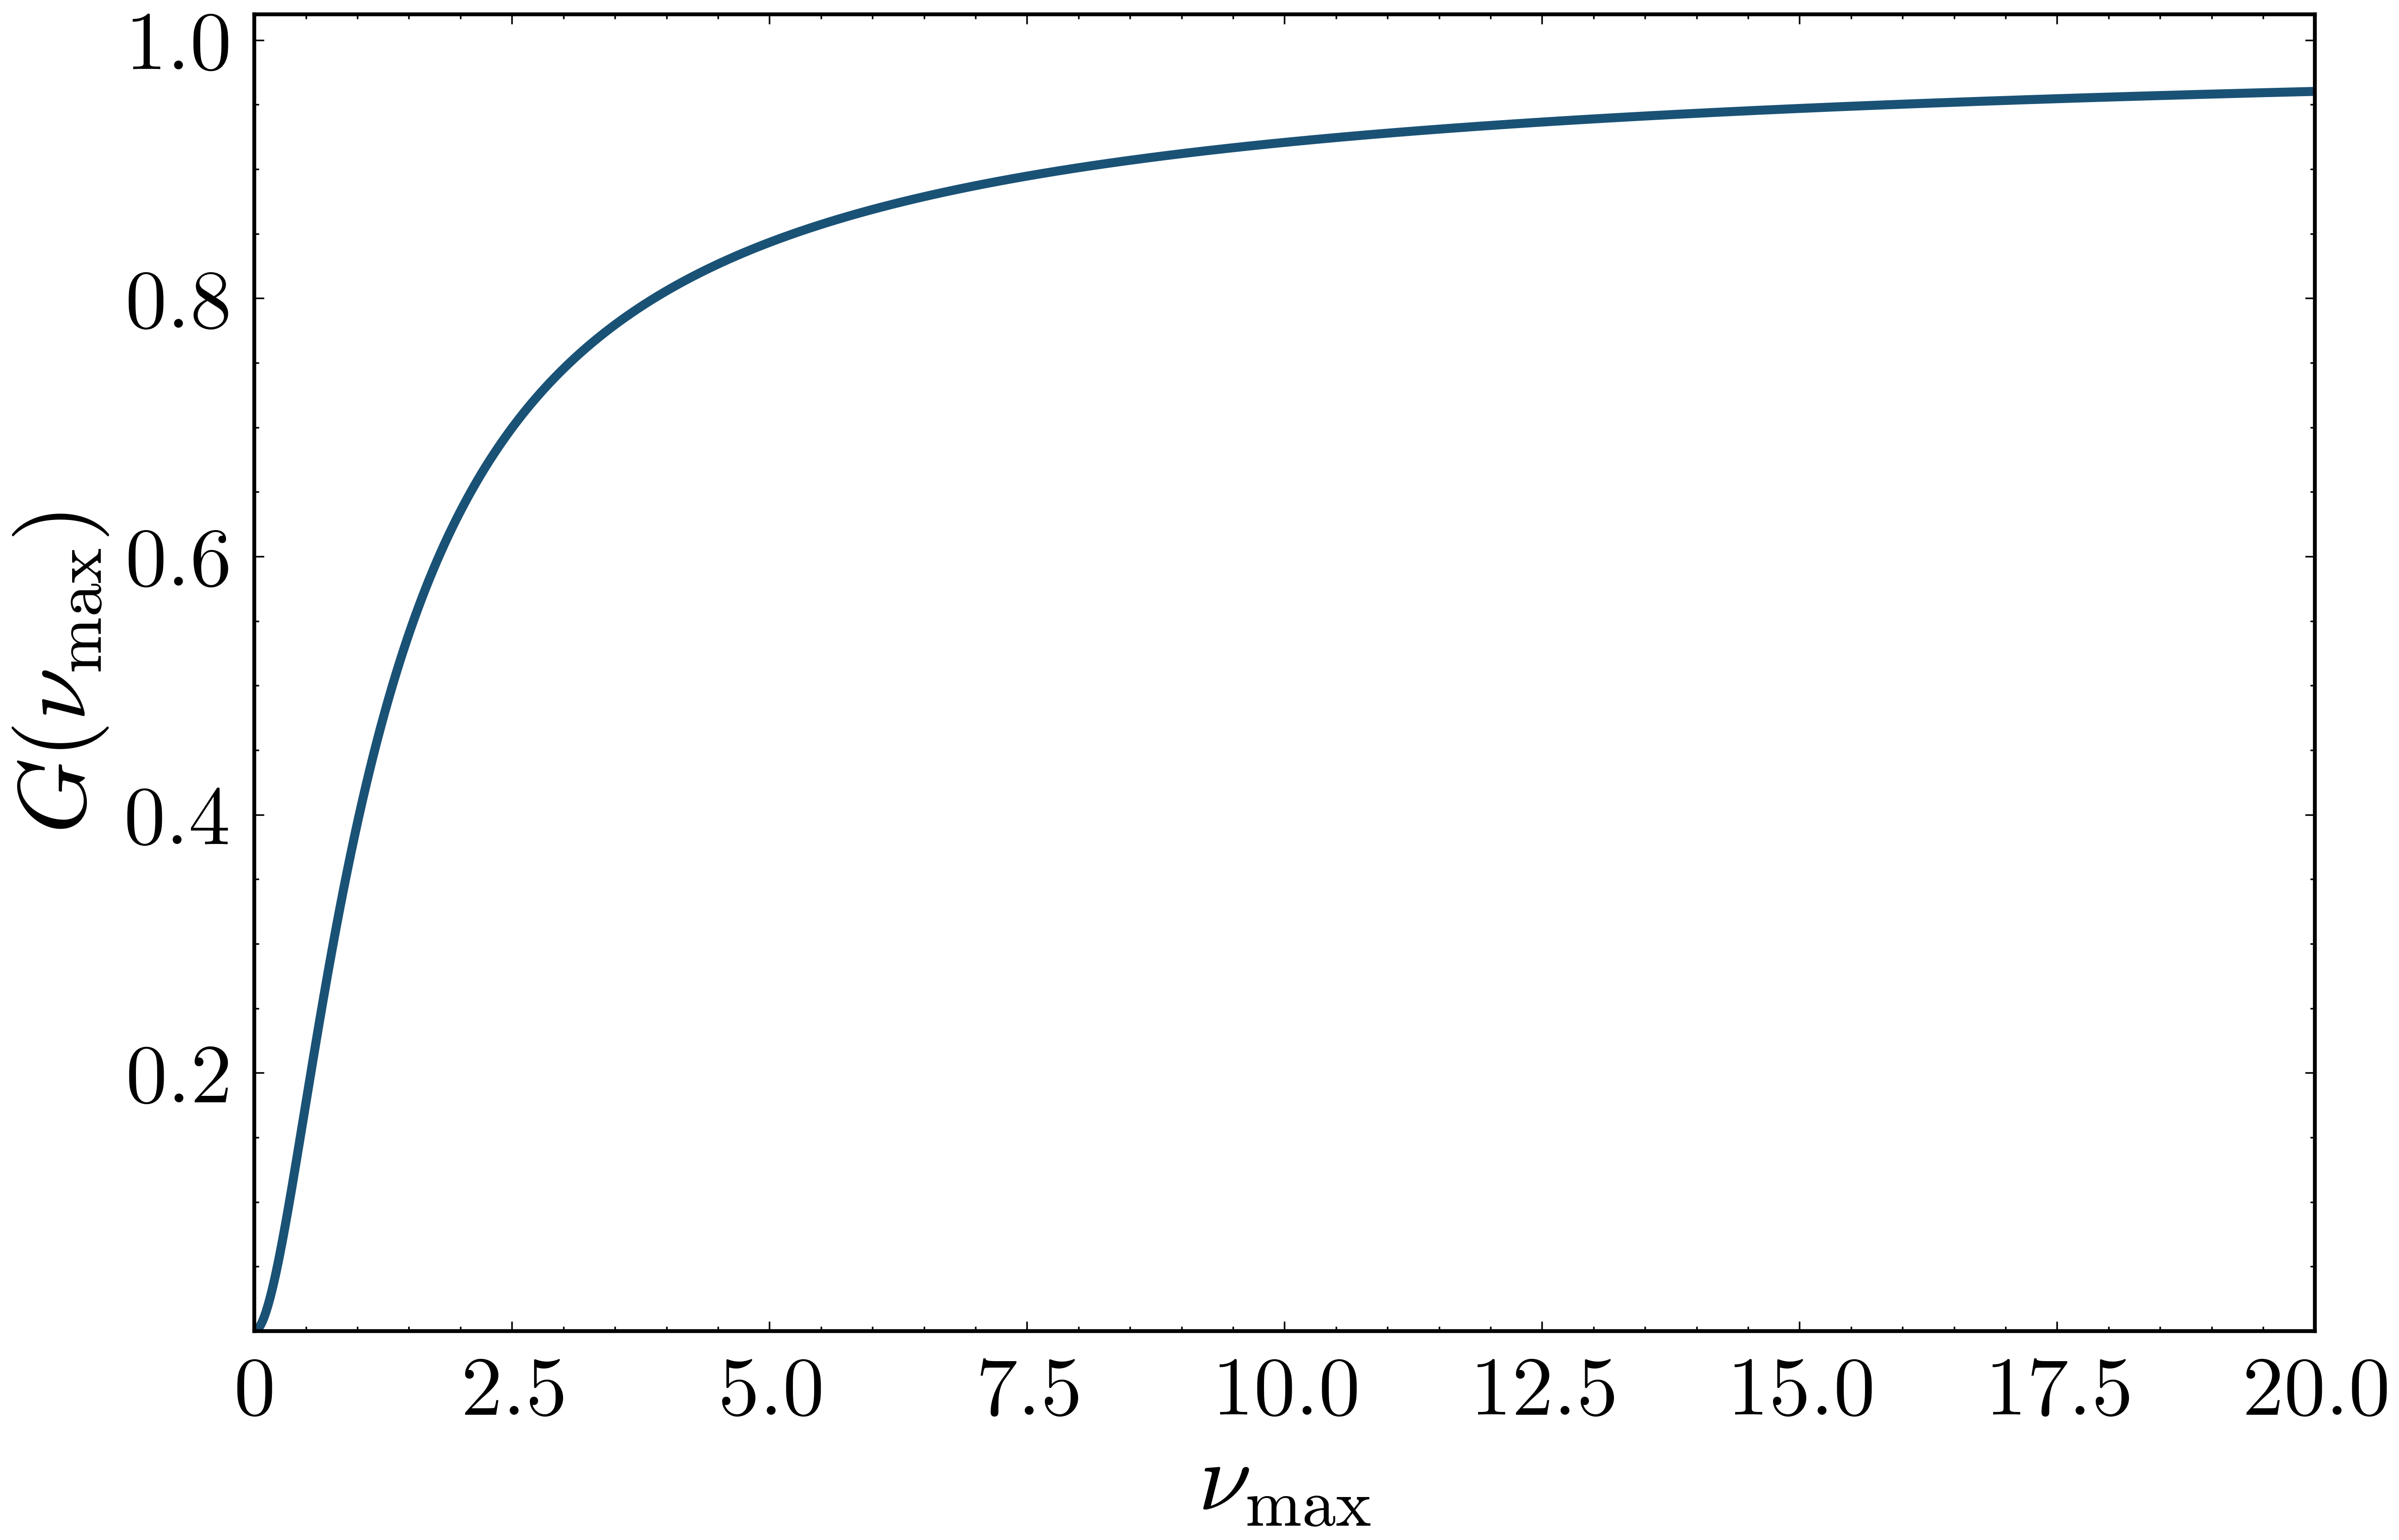
\includegraphics[width=\textwidth]{radiation_fig/spectral_weight_function_g_nu_plot.png}
		\caption{\(G(\nu)\)图像}
		\label{G(nu)图像}
		\label{G图像}
	\end{minipage}
	\hfill
	\begin{minipage}[b]{0.49\textwidth}
		\centering
		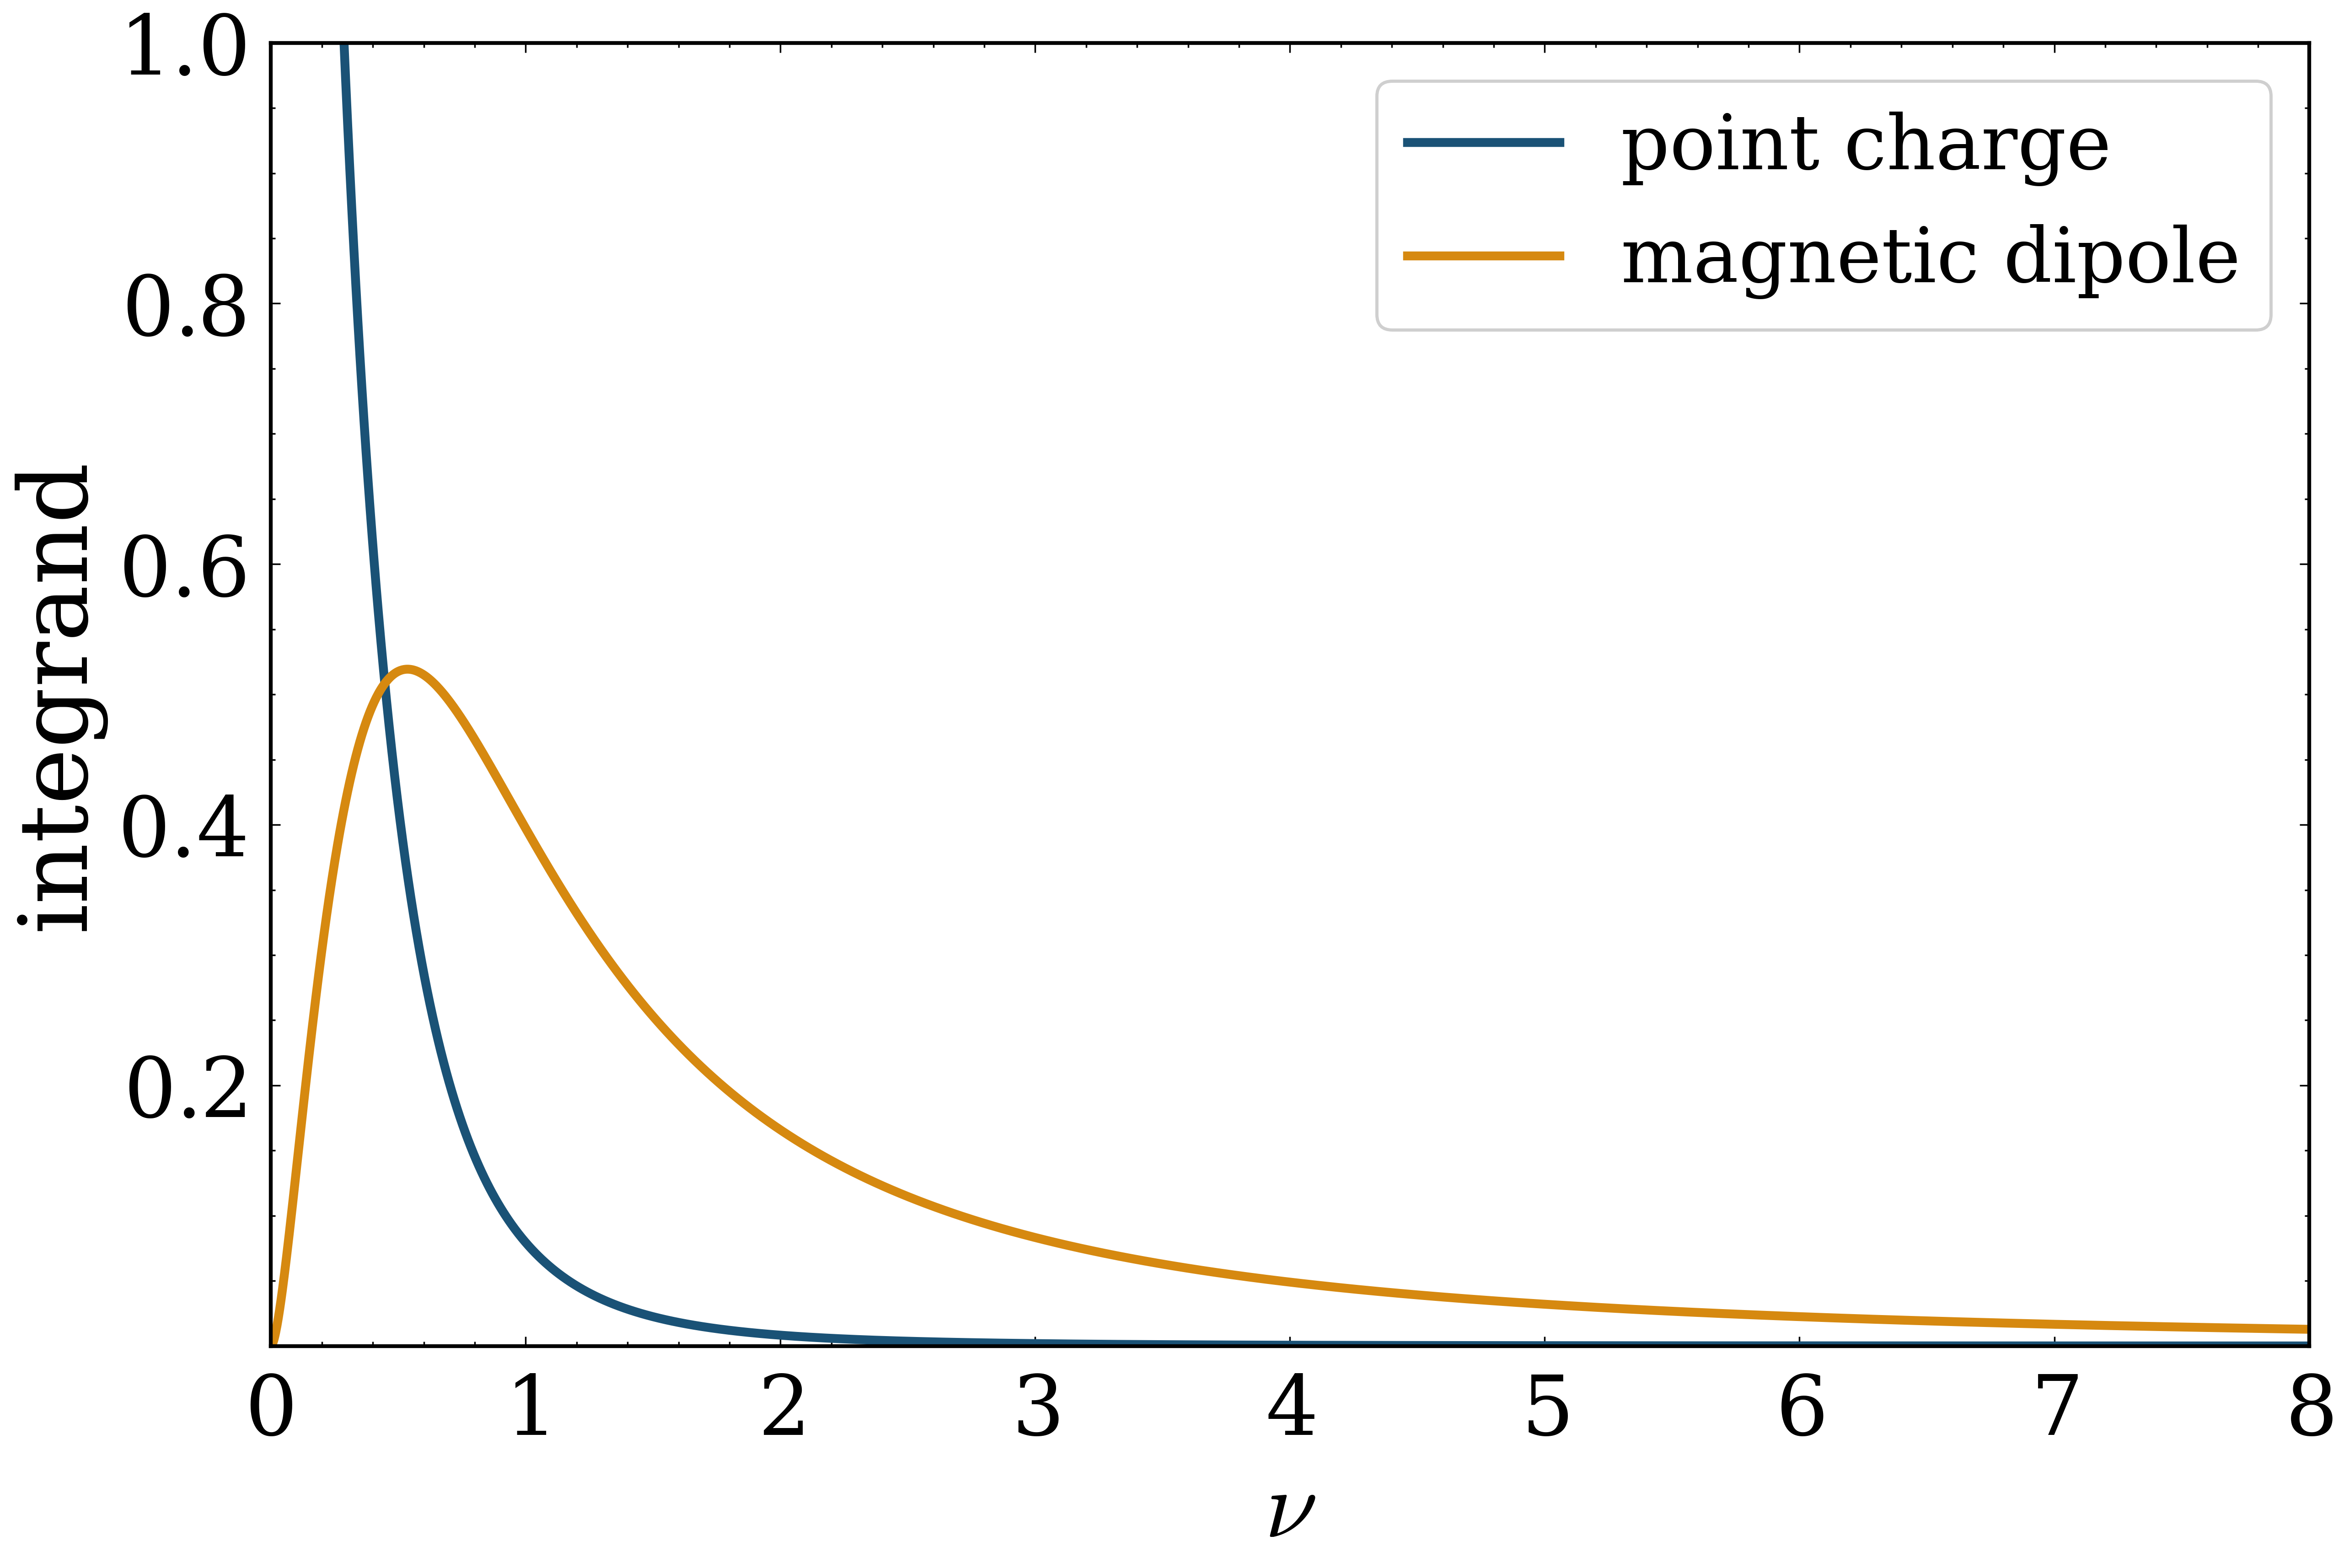
\includegraphics[width=\textwidth]{radiation_fig/charge_and_magnetic_moment_radiation_energy_spectrum.png}
		\caption{电荷及磁矩辐射能量频谱}
		\label{电荷及磁矩辐射能量频谱}
	\end{minipage}
\end{figure}
\begin{figure}[htbp]
	\centering
	\begin{subfigure}[b]{0.49\textwidth}
		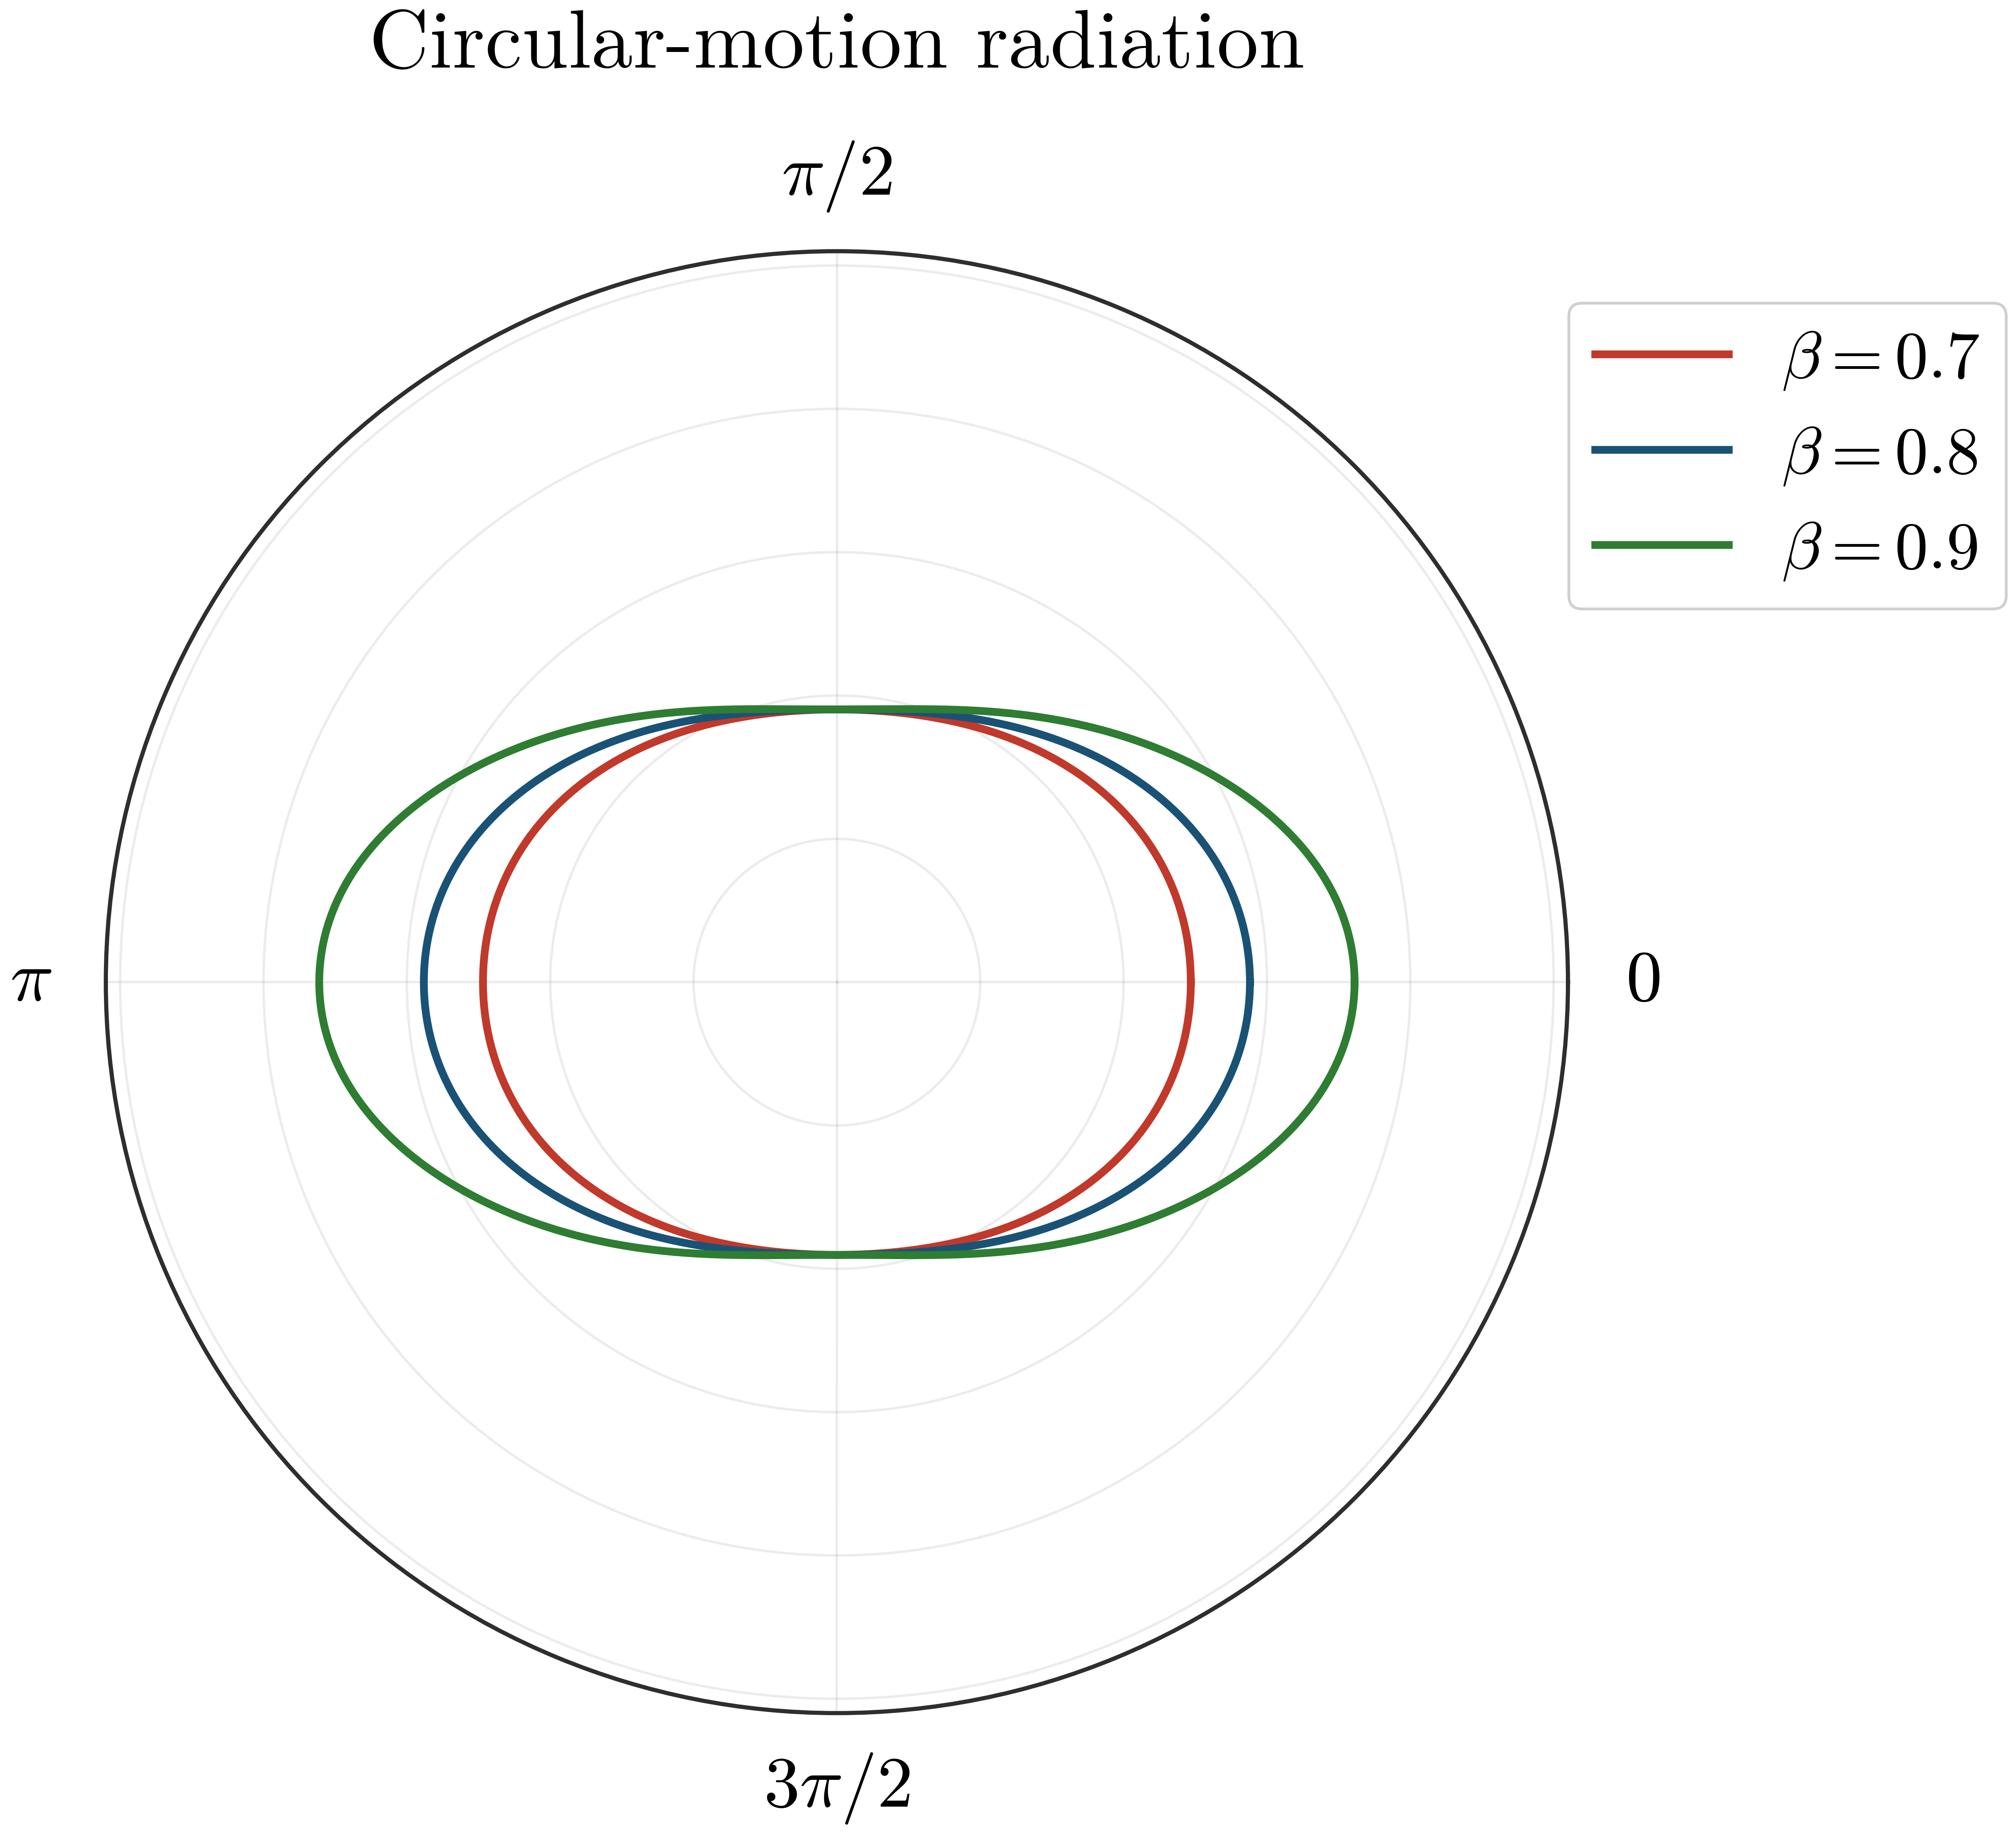
\includegraphics[width=\textwidth]{radiation_fig/circular_motion_radiation_angular_distribution.png}
		\caption{圆周运动}
		\label{点电荷周期运动辐射能量角分布-圆周运动}
	\end{subfigure}
	\hfill
	\begin{subfigure}[b]{0.49\textwidth}
		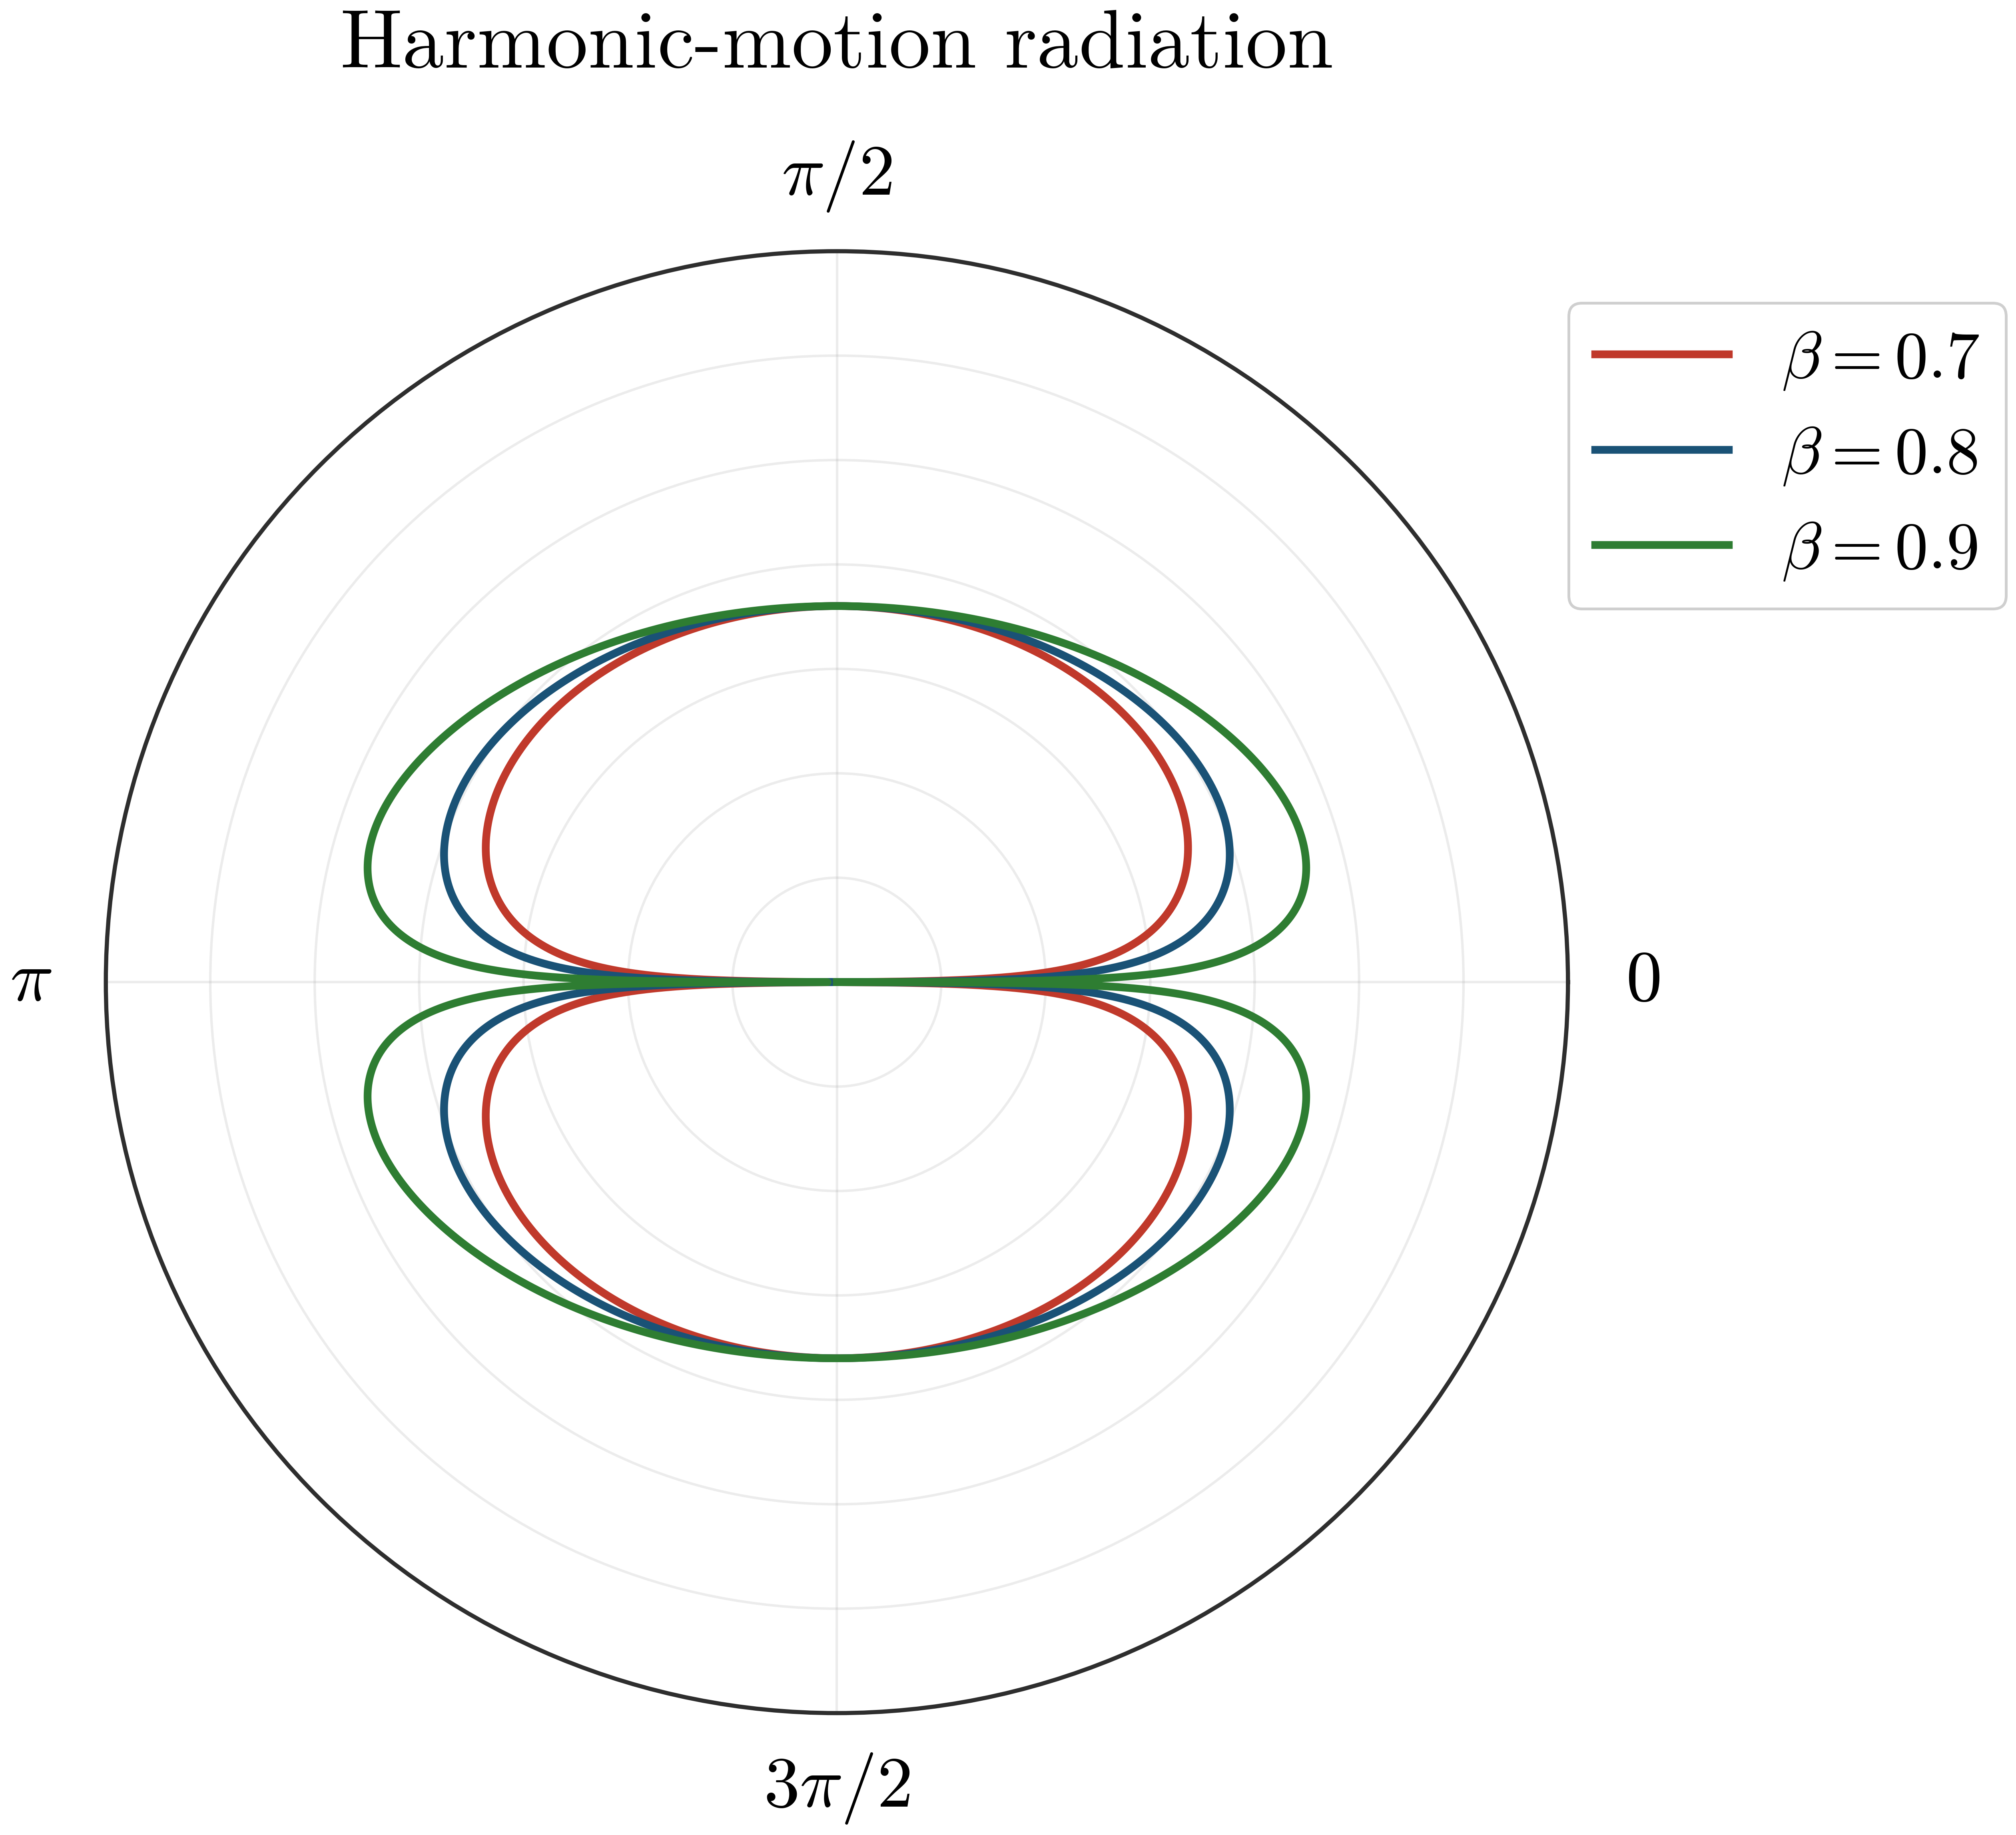
\includegraphics[width=\textwidth]{radiation_fig/harmonic_motion_radiation_angular_distribution.png}
		\caption{简谐运动}
		\label{点电荷周期运动辐射能量角分布-简谐运动}
	\end{subfigure}
	\caption{点电荷周期运动辐射能量角分布}
	\label{点电荷周期运动辐射能量角分布}
\end{figure}
\begin{figure}[htbp]
	\centering
	\begin{subfigure}[b]{0.23\textwidth}
		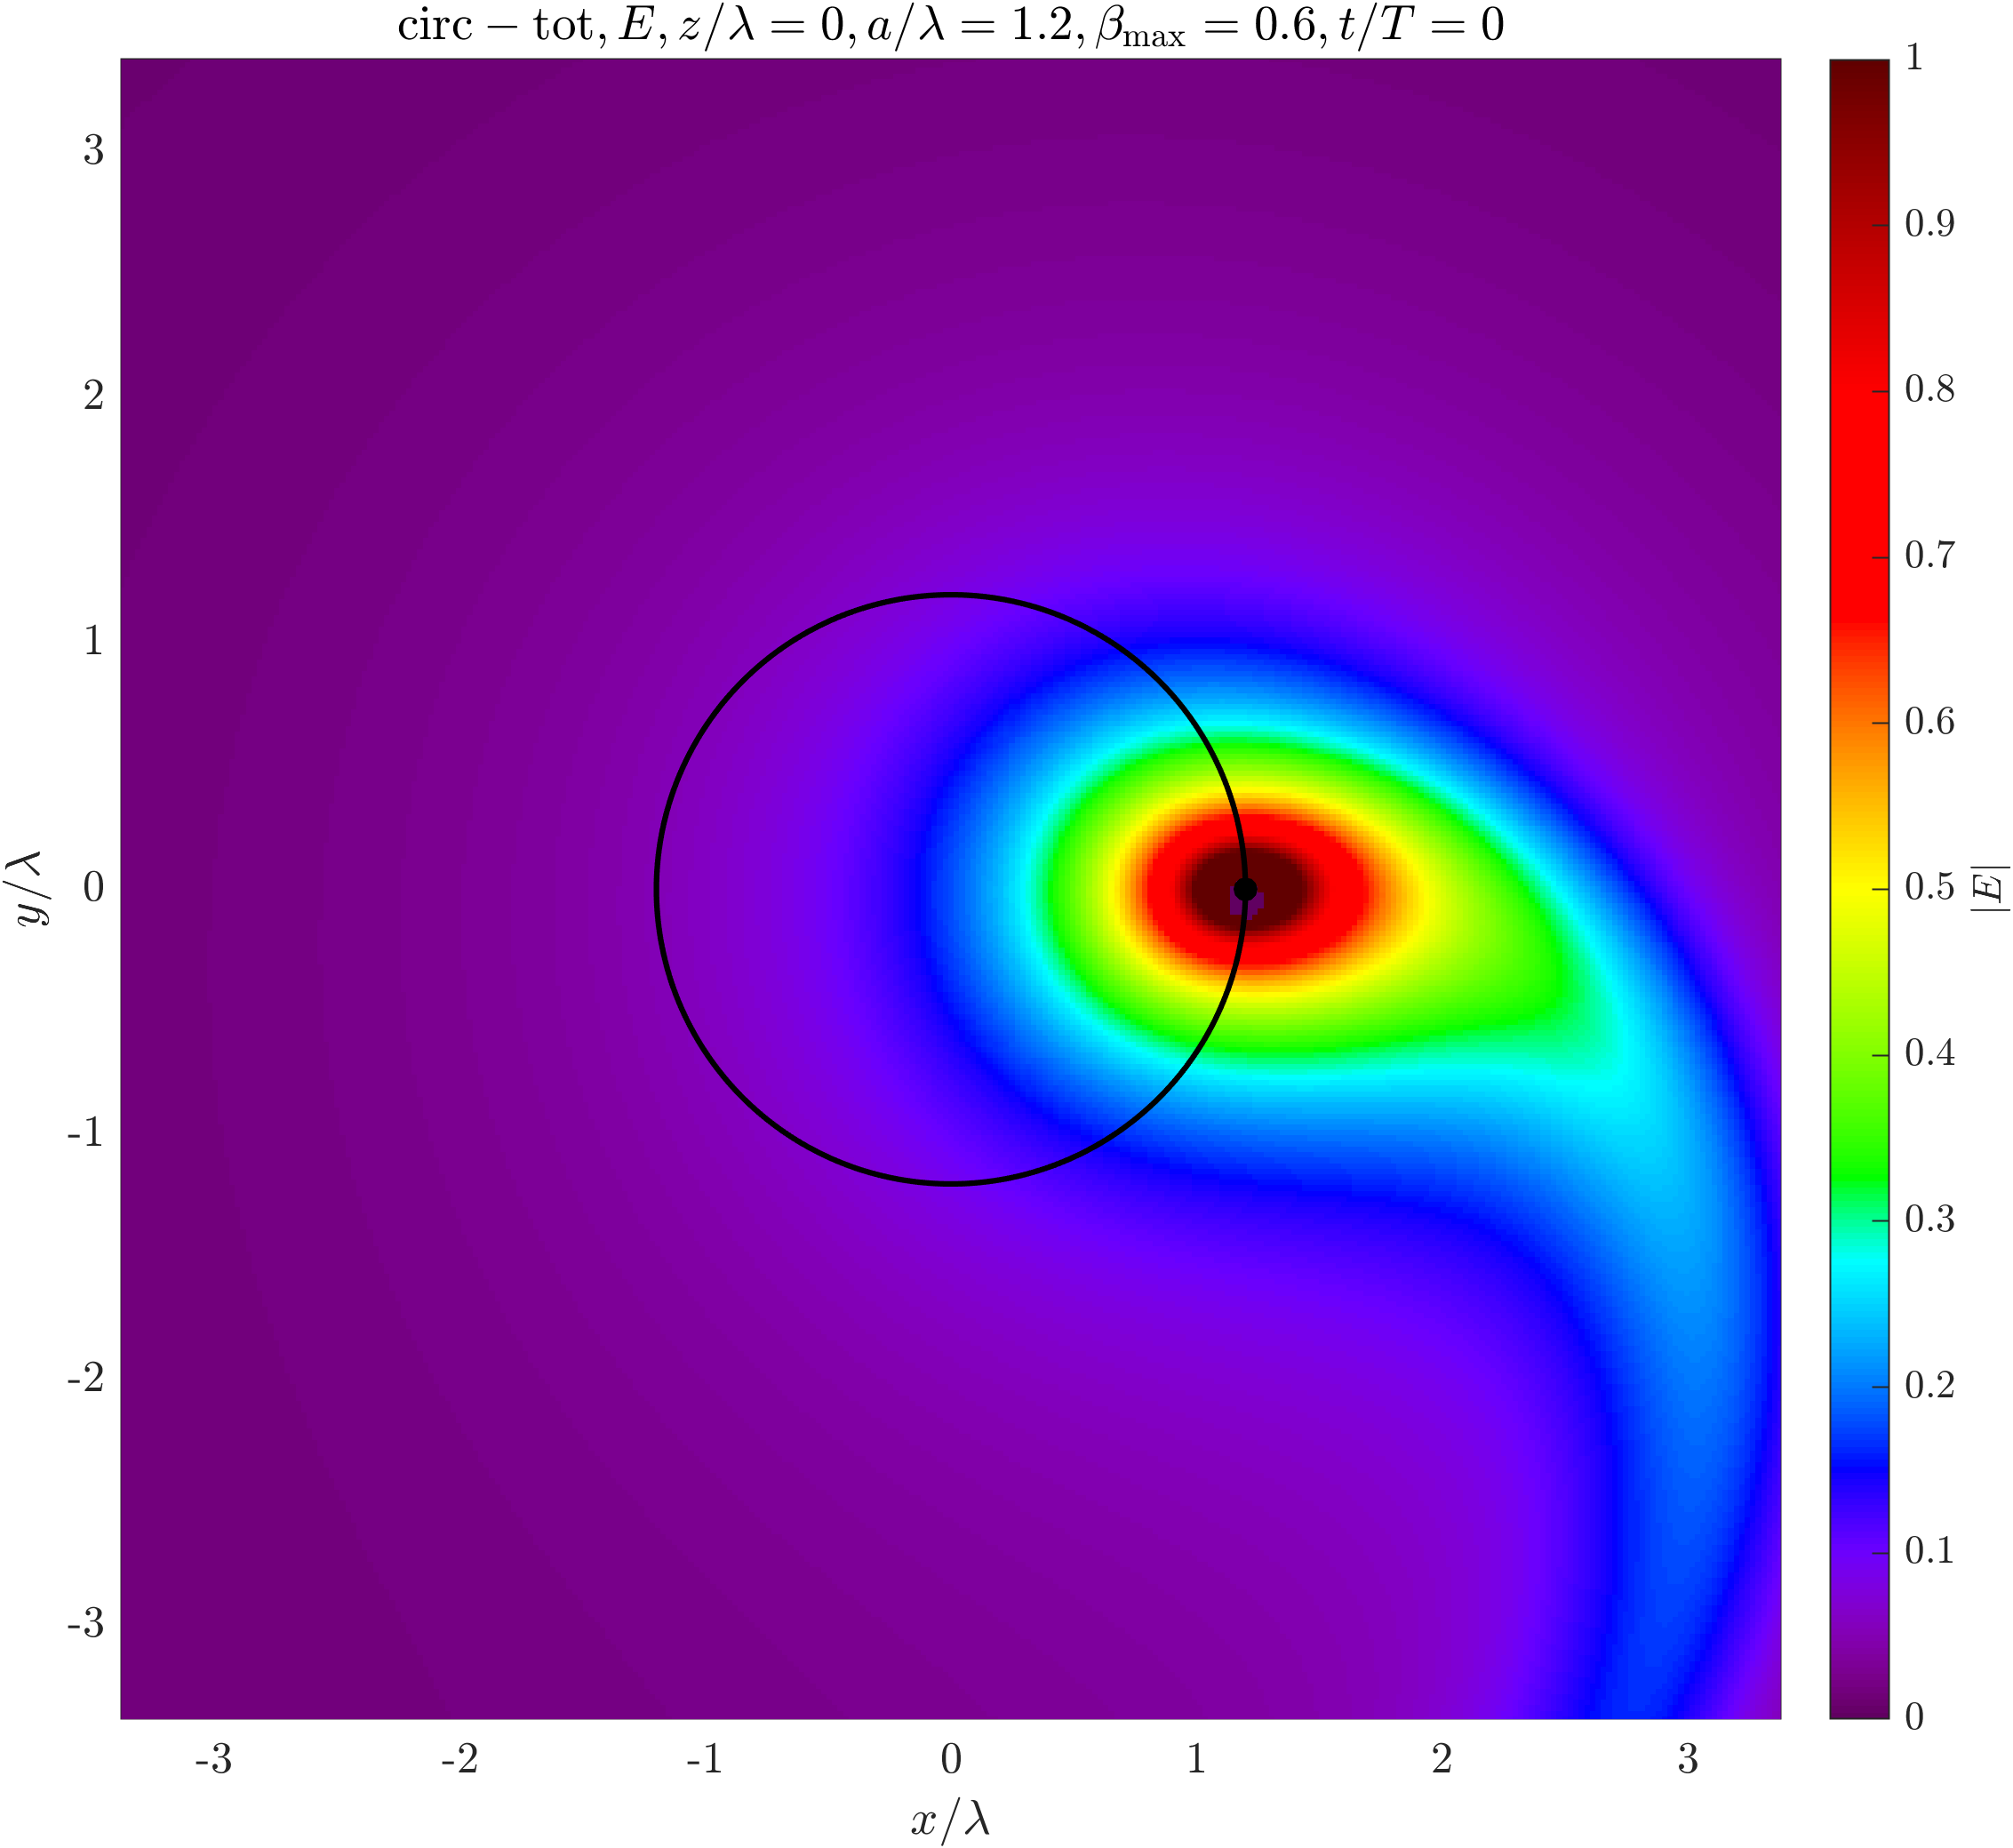
\includegraphics[width=\textwidth]{radiation_fig/circular_motion_e_xy_beta_0_6.png}
		\caption{\(E|_{xy}\) (\(\beta=0.6\))}
		\label{点电荷圆周运动辐射场示意图-E|_xy(beta=0.6)}
	\end{subfigure}
	\hfill
	\begin{subfigure}[b]{0.23\textwidth}
		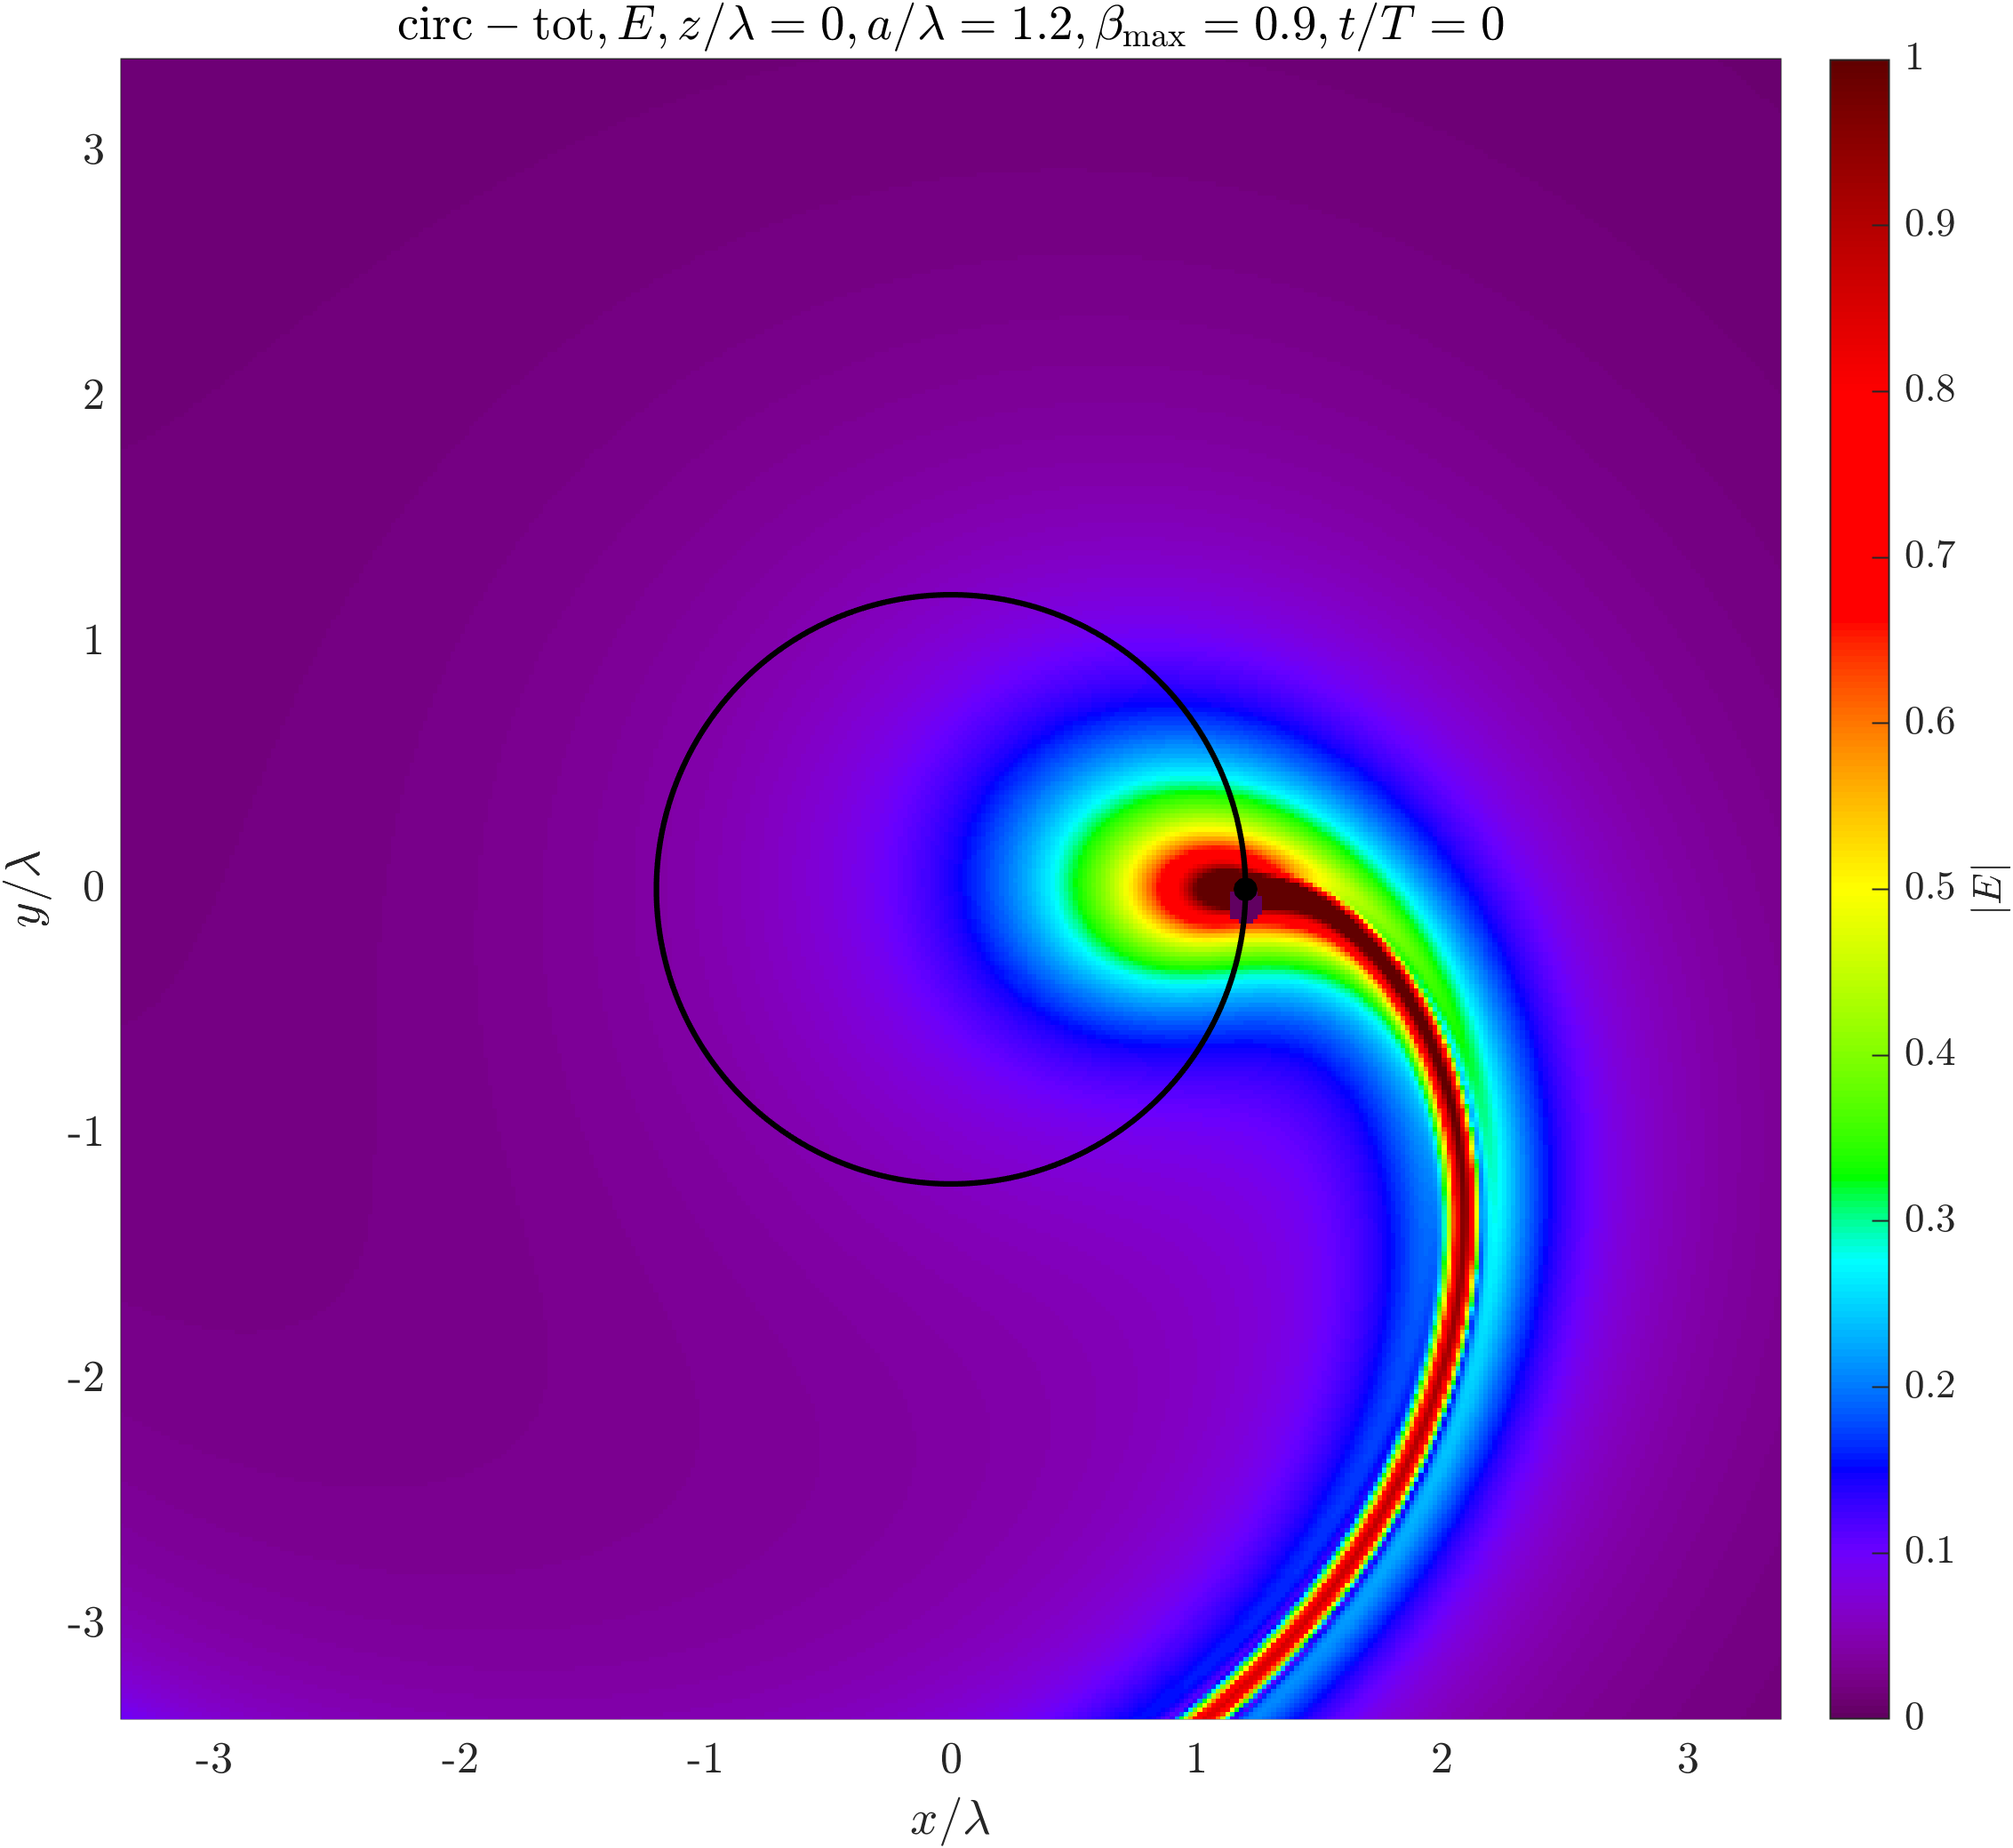
\includegraphics[width=\textwidth]{radiation_fig/circular_motion_e_xy_beta_0_9.png}
		\caption{\(E|_{xy}\) (\(\beta=0.9\))}
		\label{点电荷圆周运动辐射场示意图-E|_xy(beta=0.9)}
	\end{subfigure}
	\hfill
	\begin{subfigure}[b]{0.23\textwidth}
		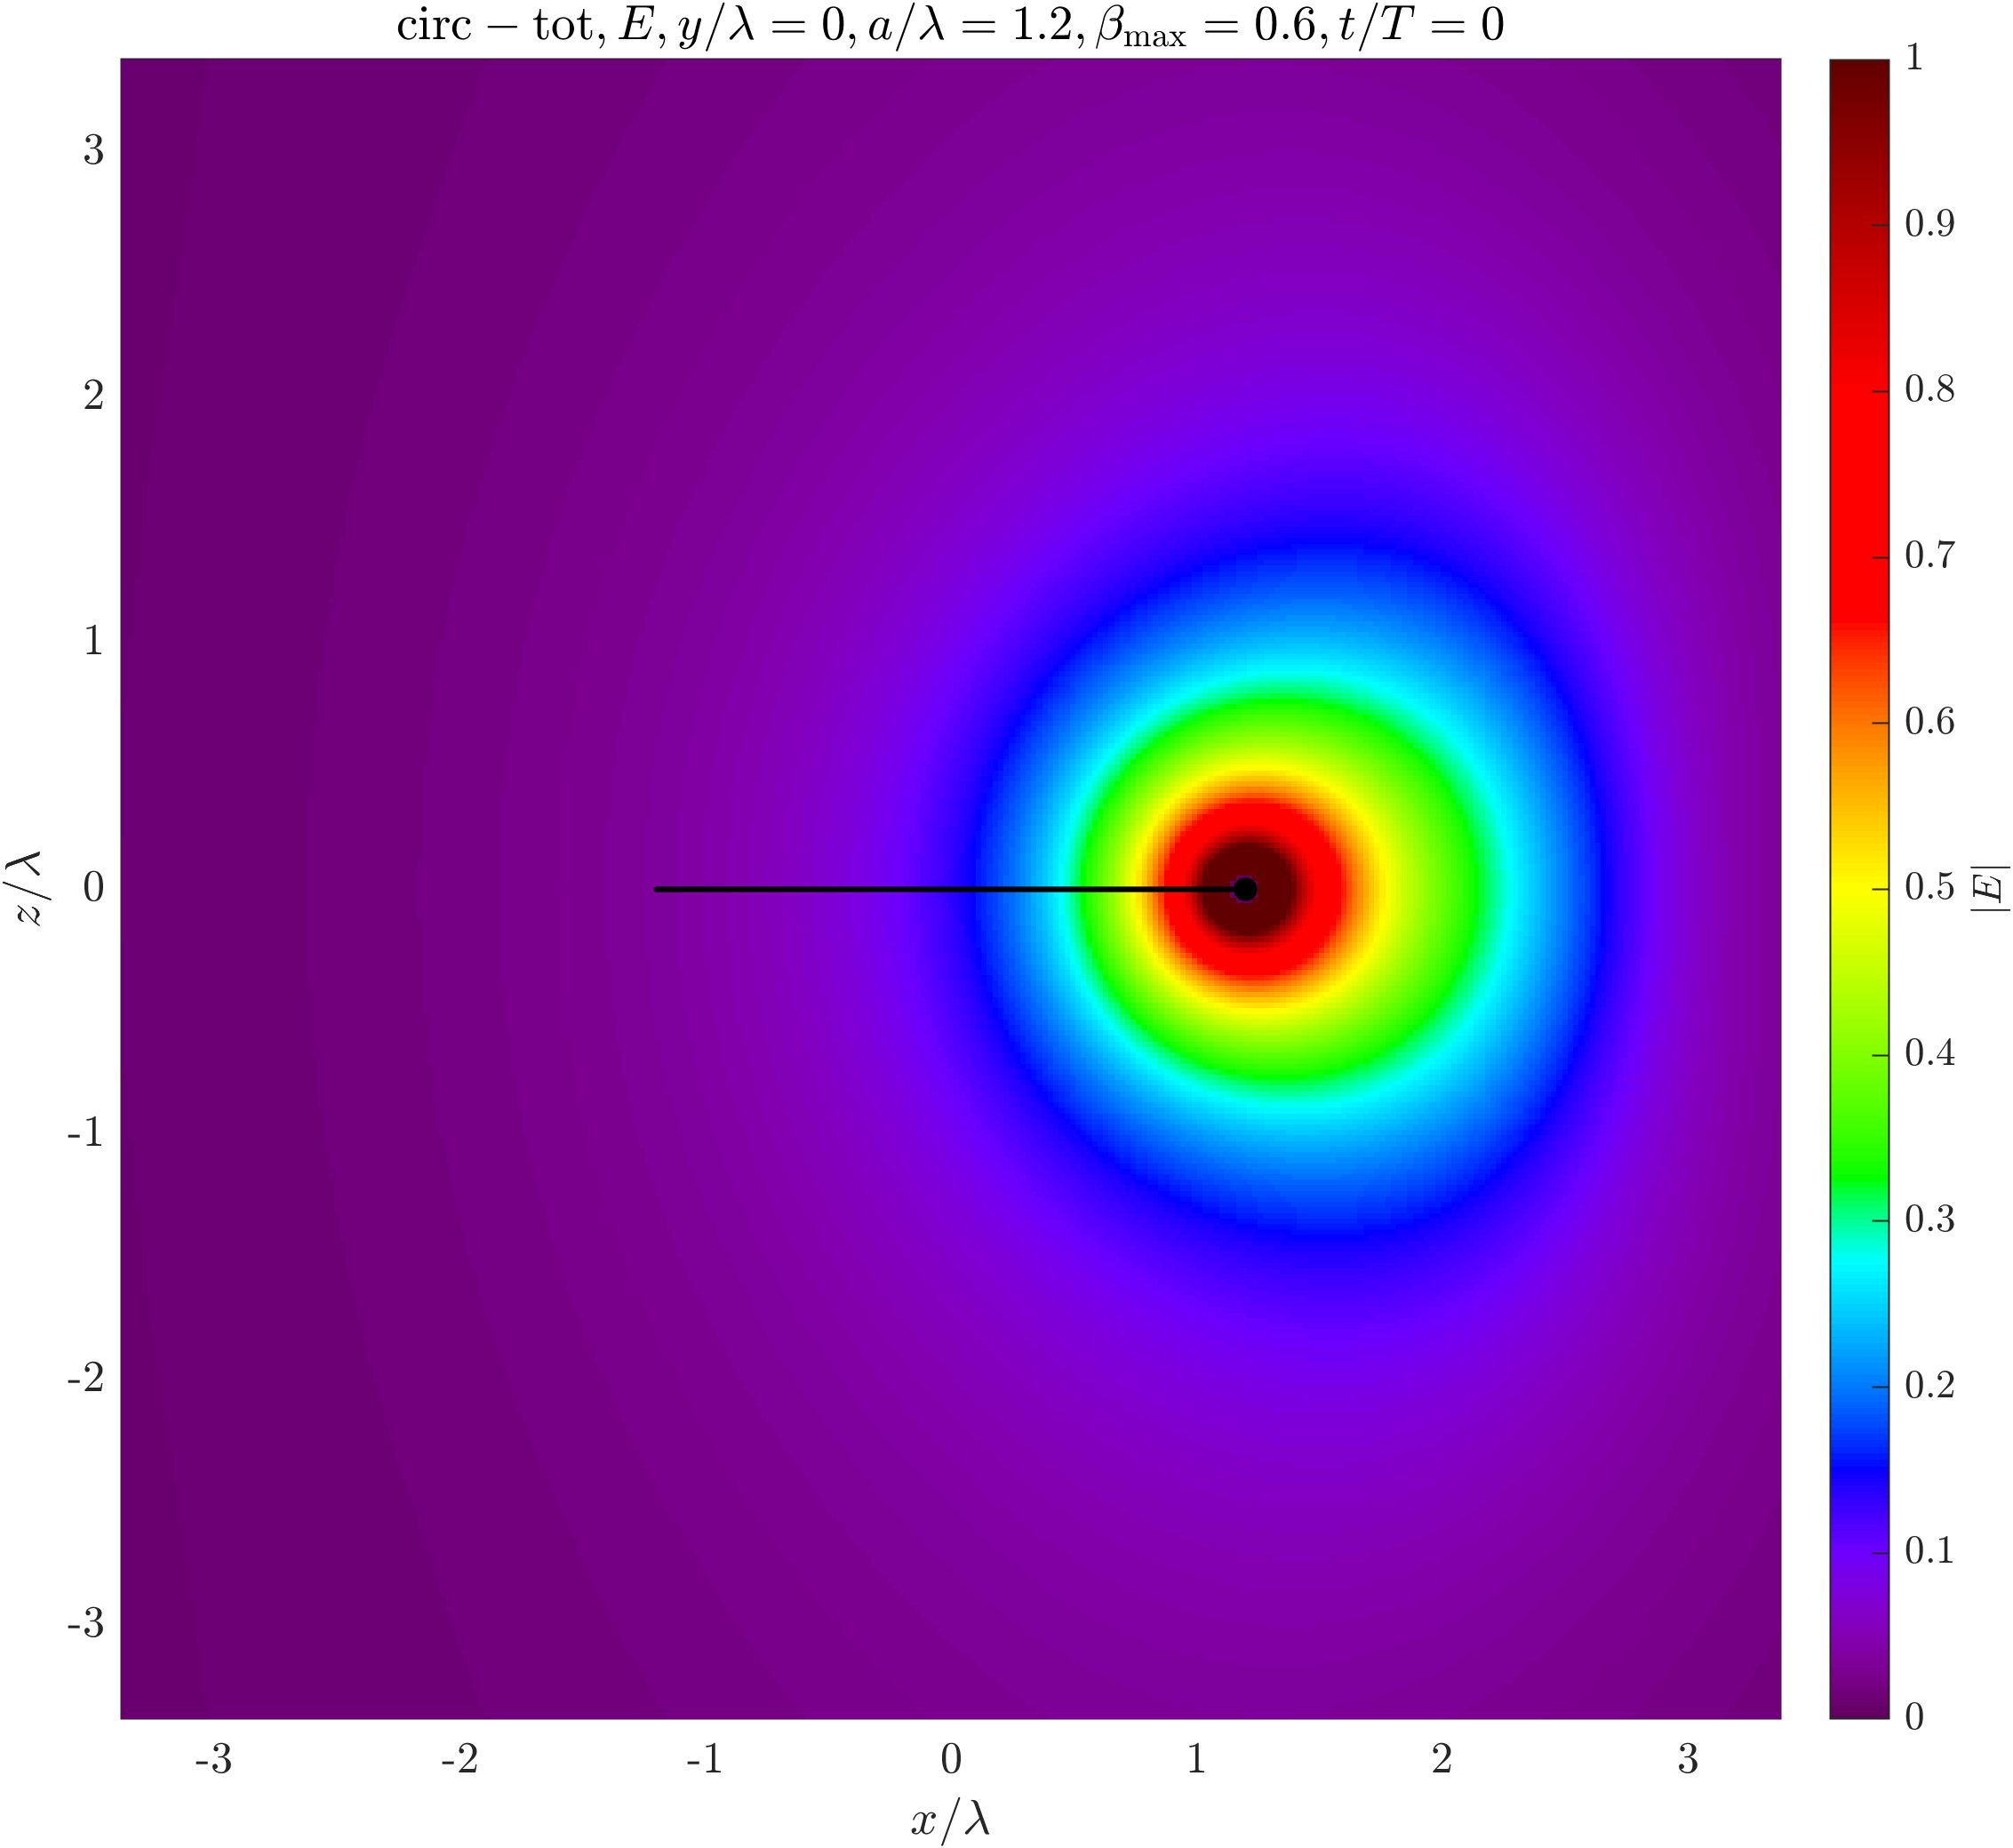
\includegraphics[width=\textwidth]{radiation_fig/circular_motion_e_xz_beta_0_6.png}
		\caption{\(E|_{xz}\) (\(\beta=0.6\))}
		\label{点电荷圆周运动辐射场示意图-E|_xz(beta=0.6)}
	\end{subfigure}
	\hfill
	\begin{subfigure}[b]{0.23\textwidth}
		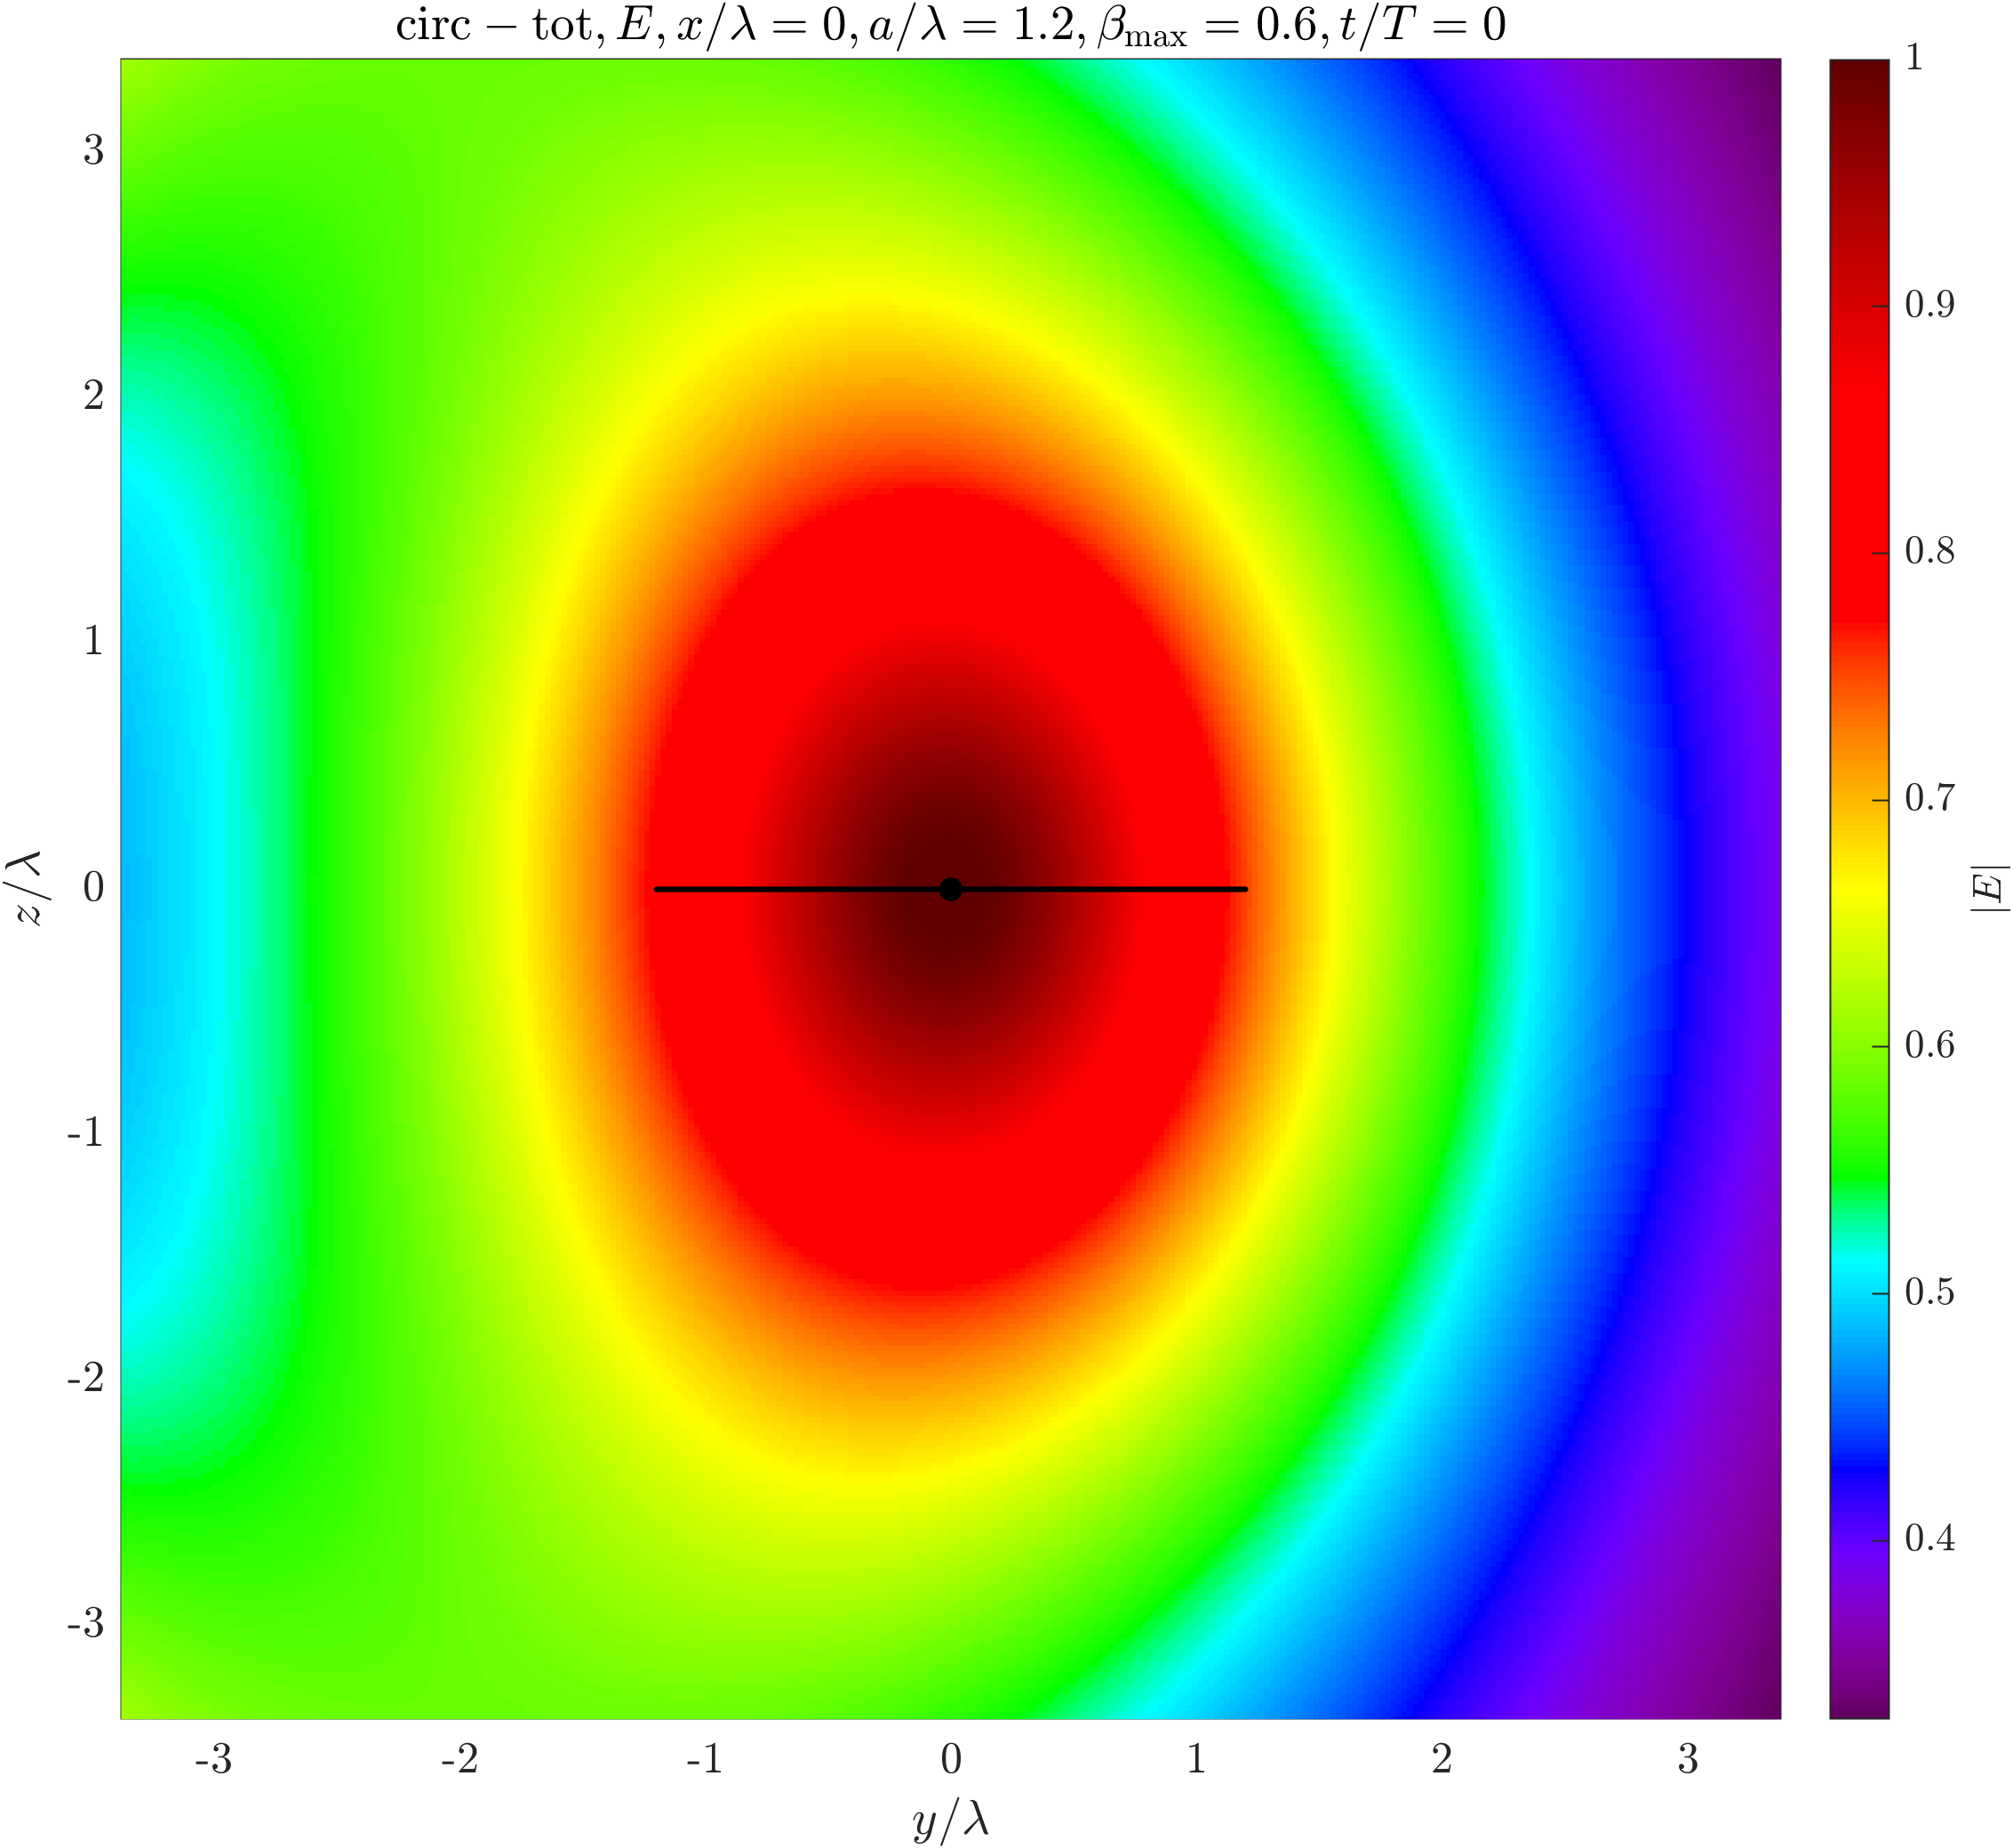
\includegraphics[width=\textwidth]{radiation_fig/circular_motion_e_yz_beta_0_6.png}
		\caption{\(E|_{yz}\) (\(\beta=0.6\))}
		\label{点电荷圆周运动辐射场示意图-E|_yz(beta=0.6)}
	\end{subfigure}
	\vspace{0.2cm}
	\begin{subfigure}[b]{0.23\textwidth}
		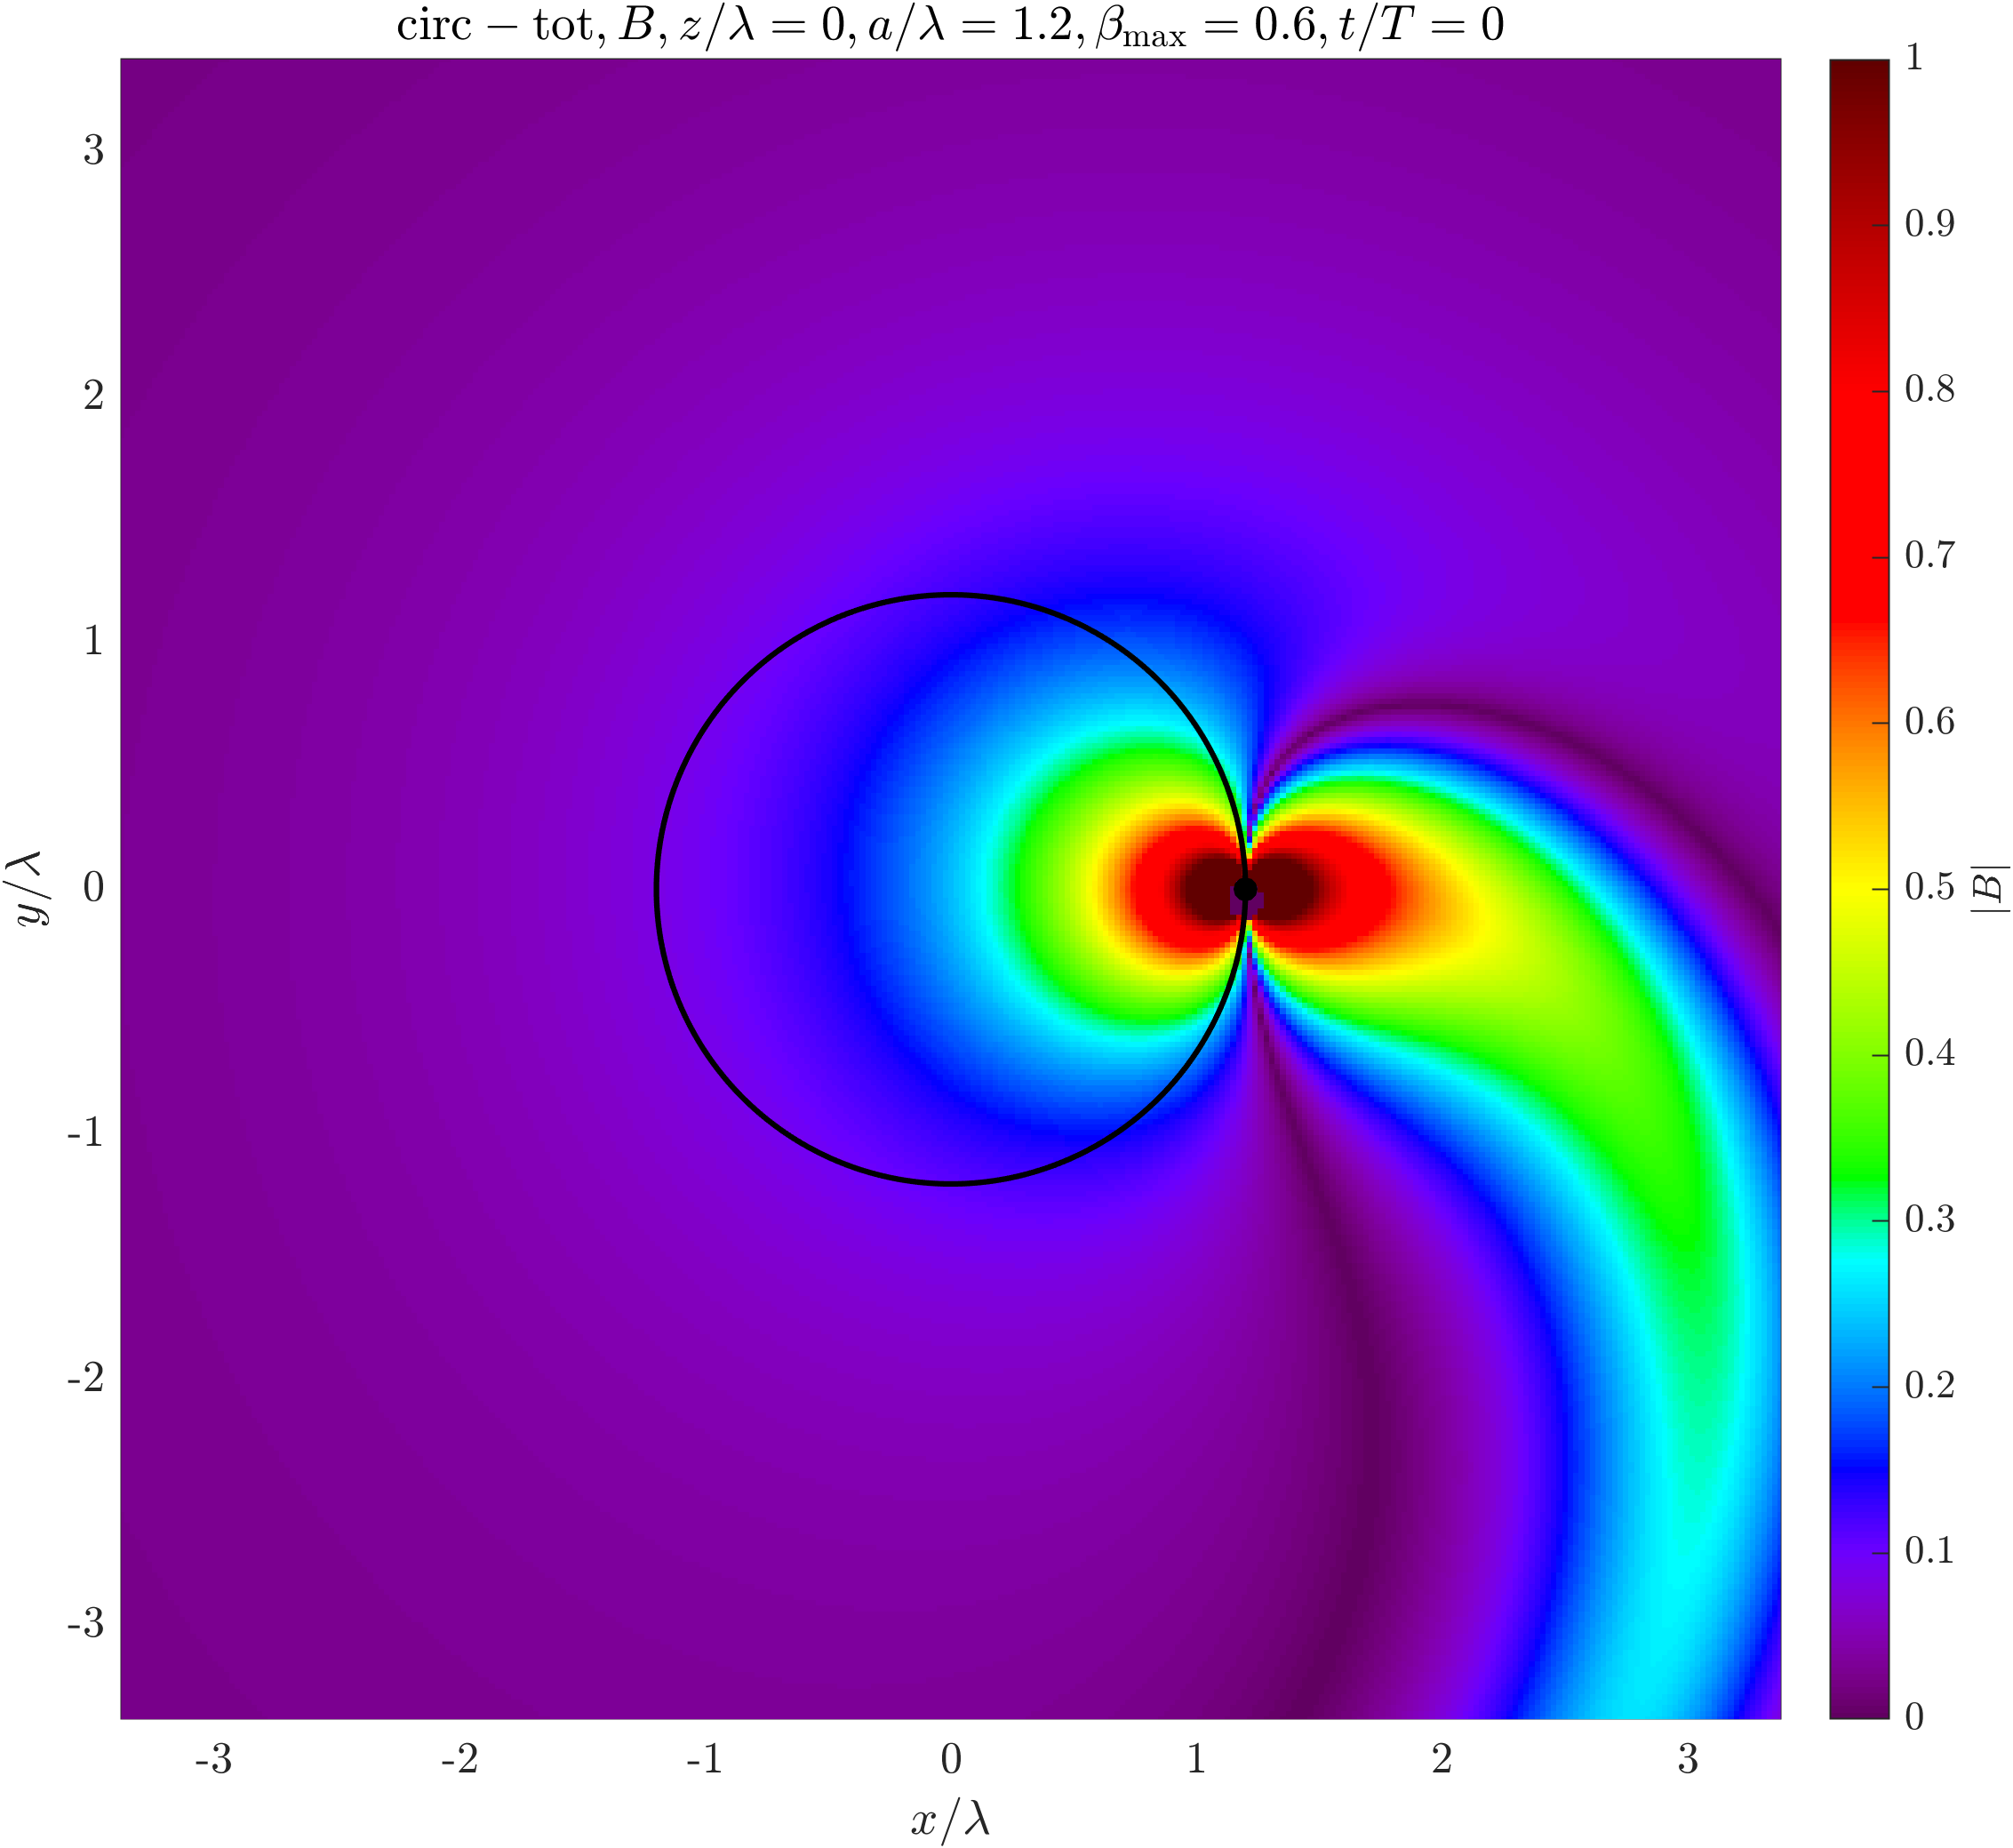
\includegraphics[width=\textwidth]{radiation_fig/circular_motion_b_xy_beta_0_6.png}
		\caption{\(B|_{xy}\) (\(\beta=0.6\))}
		\label{点电荷圆周运动辐射场示意图-B|_xy(beta=0.6)}
	\end{subfigure}
	\hfill
	\begin{subfigure}[b]{0.23\textwidth}
		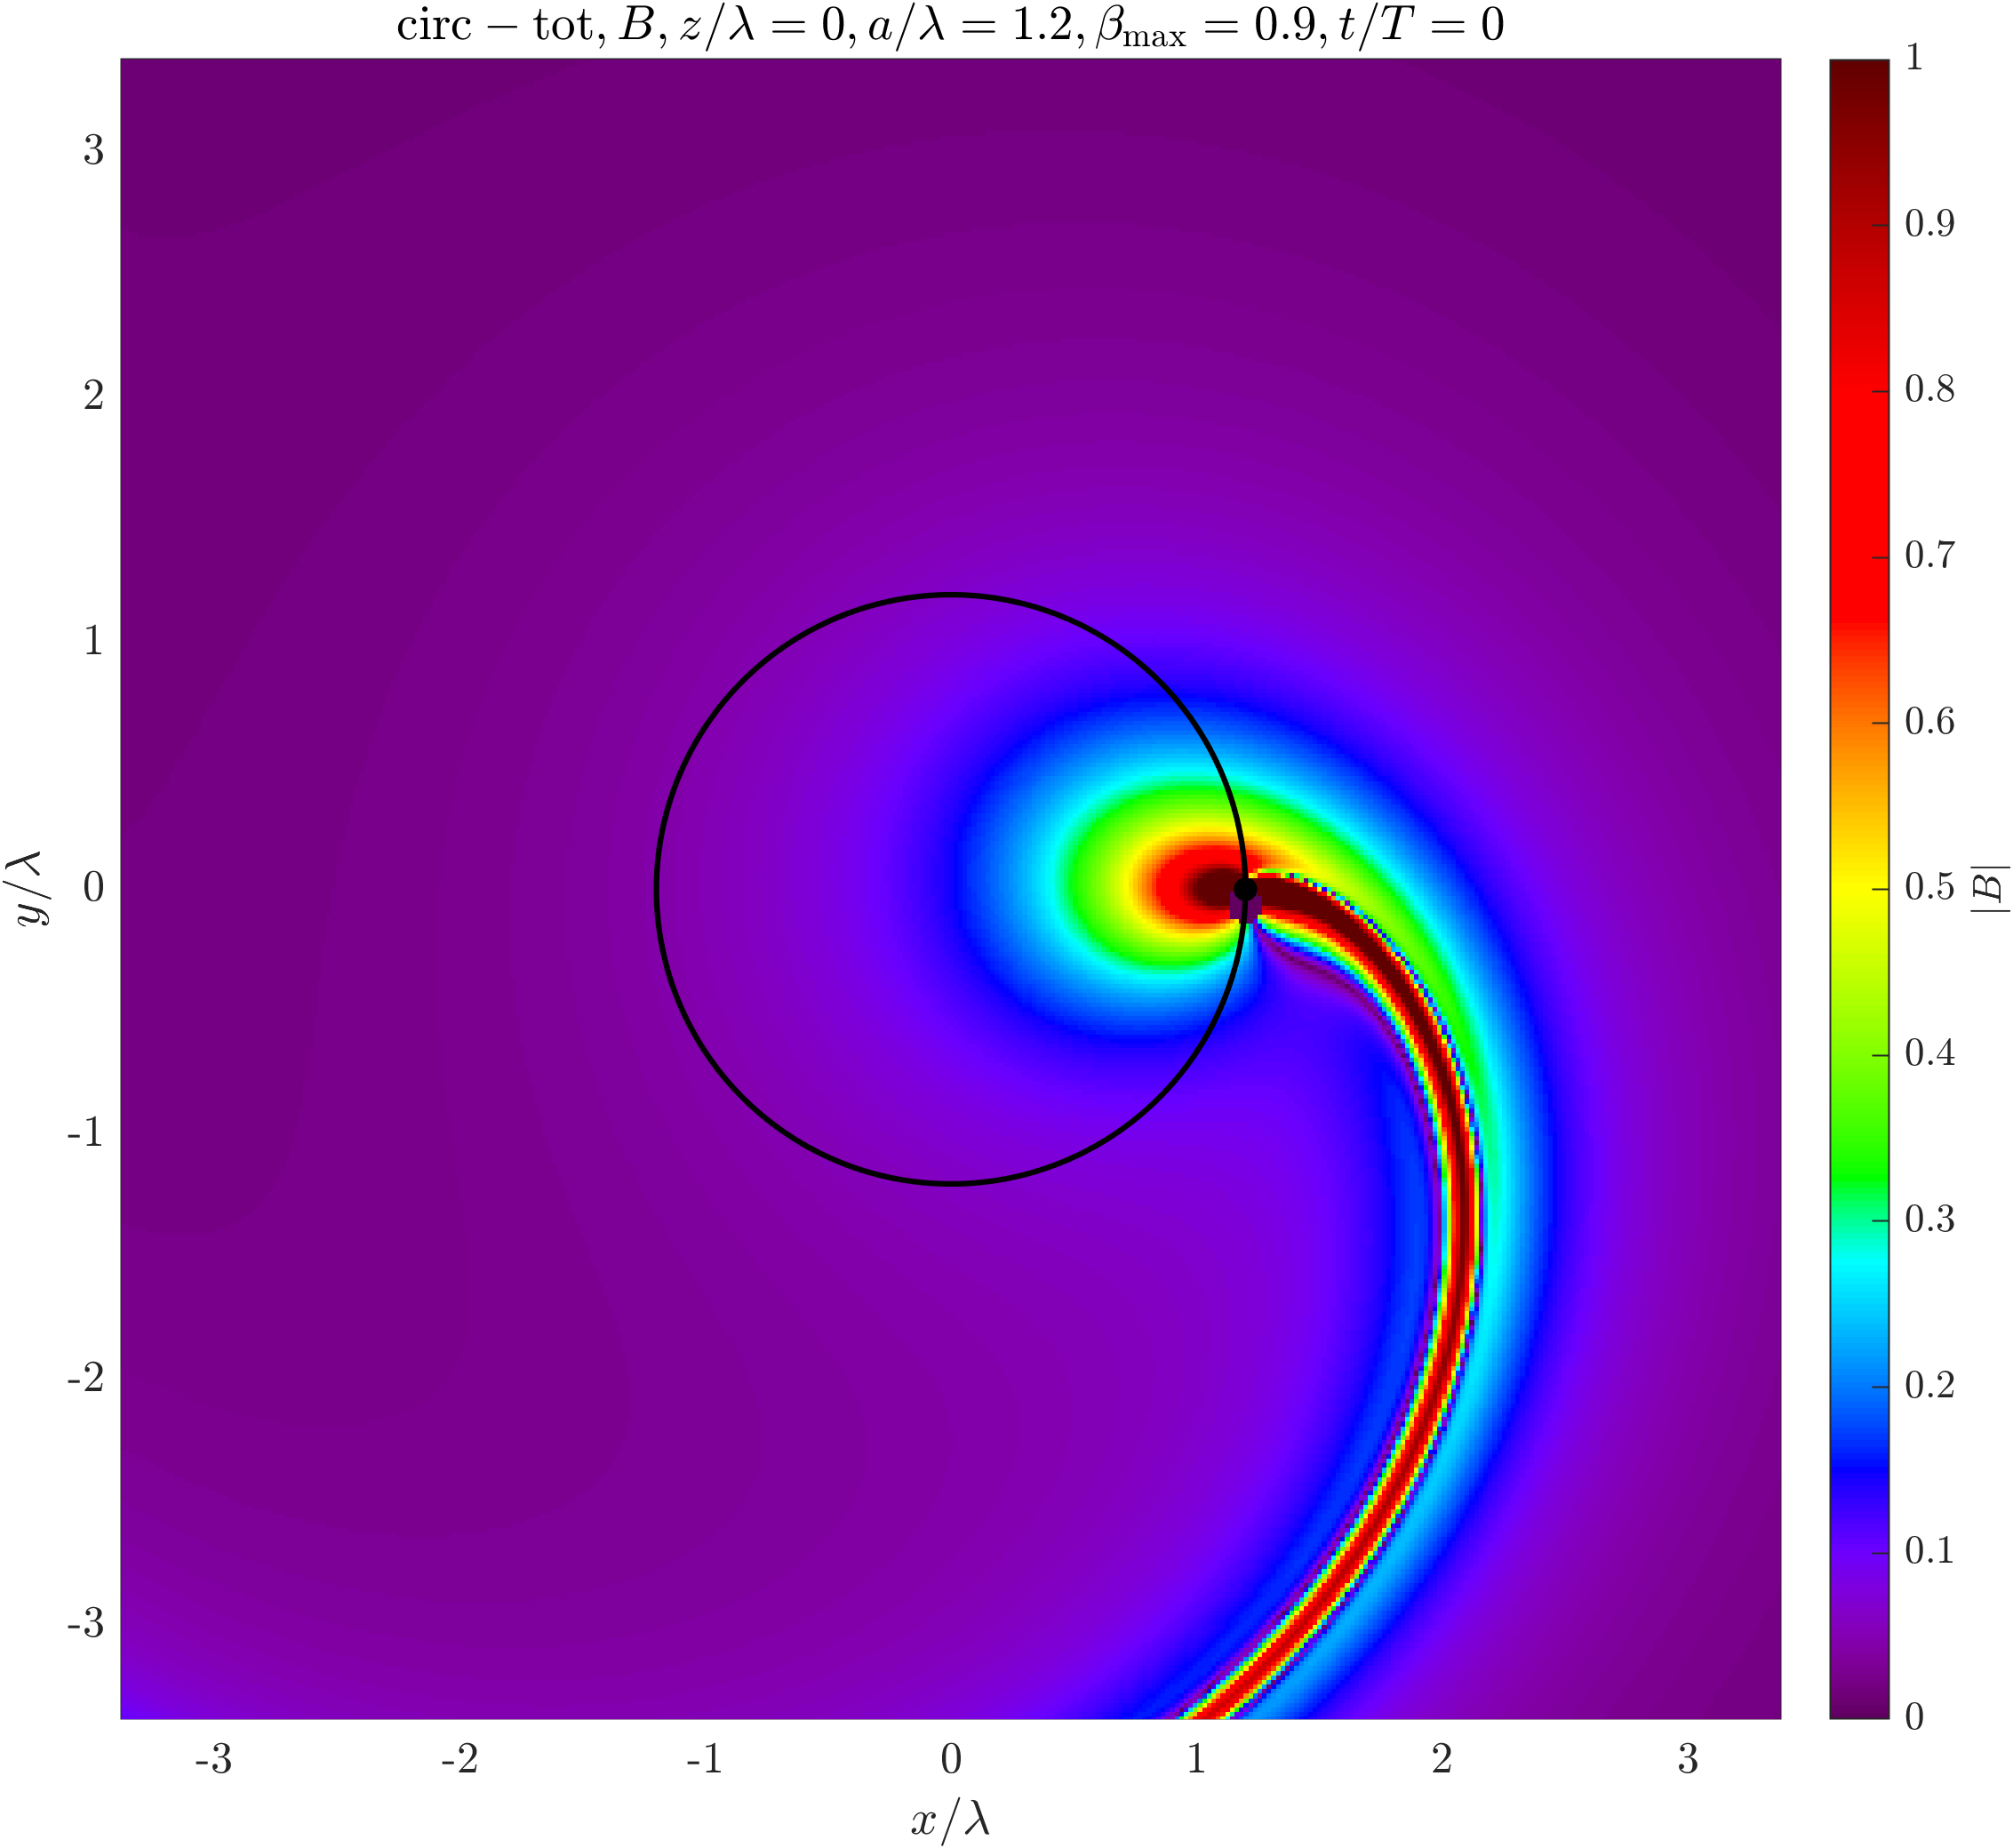
\includegraphics[width=\textwidth]{radiation_fig/circular_motion_b_xy_beta_0_9.png}
		\caption{\(B|_{xy}\) (\(\beta=0.9\))}
		\label{点电荷圆周运动辐射场示意图-B|_xy(beta=0.9)}
	\end{subfigure}
	\hfill
	\begin{subfigure}[b]{0.23\textwidth}
		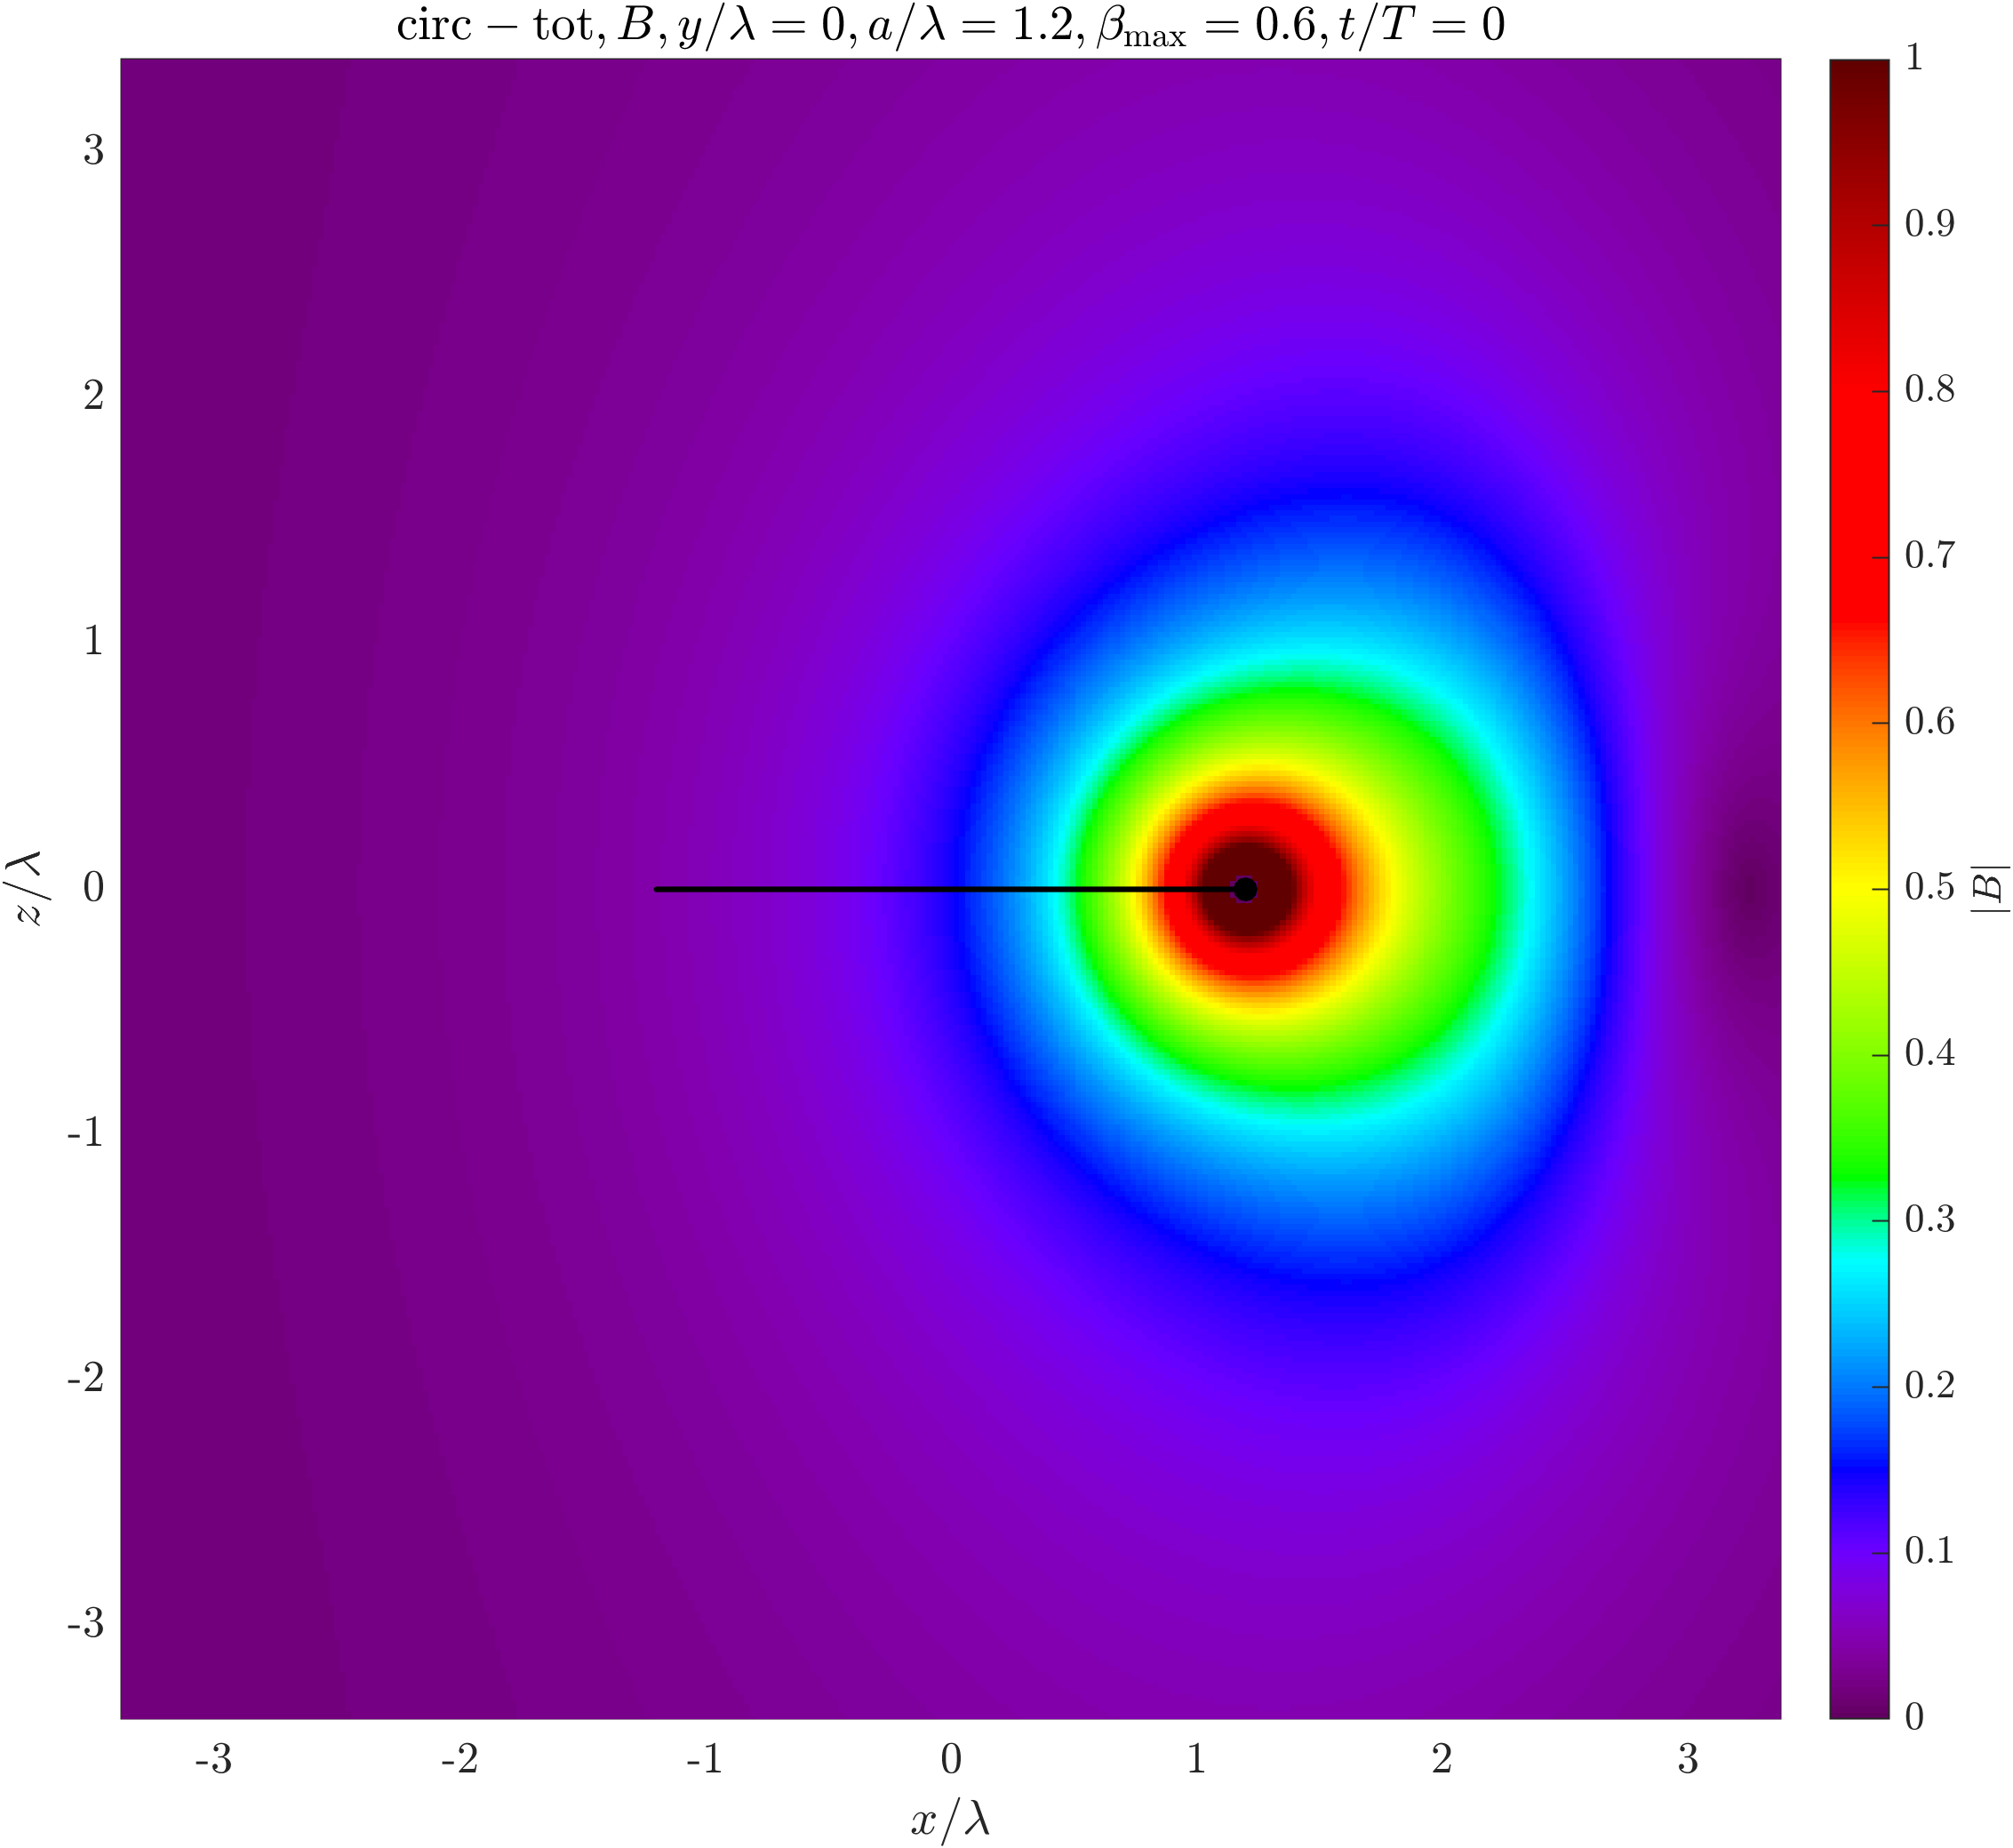
\includegraphics[width=\textwidth]{radiation_fig/circular_motion_b_xz_beta_0_6.png}
		\caption{\(B|_{xz}\) (\(\beta=0.6\))}
		\label{点电荷圆周运动辐射场示意图-B|_xz(beta=0.6)}
	\end{subfigure}
	\hfill
	\begin{subfigure}[b]{0.23\textwidth}
		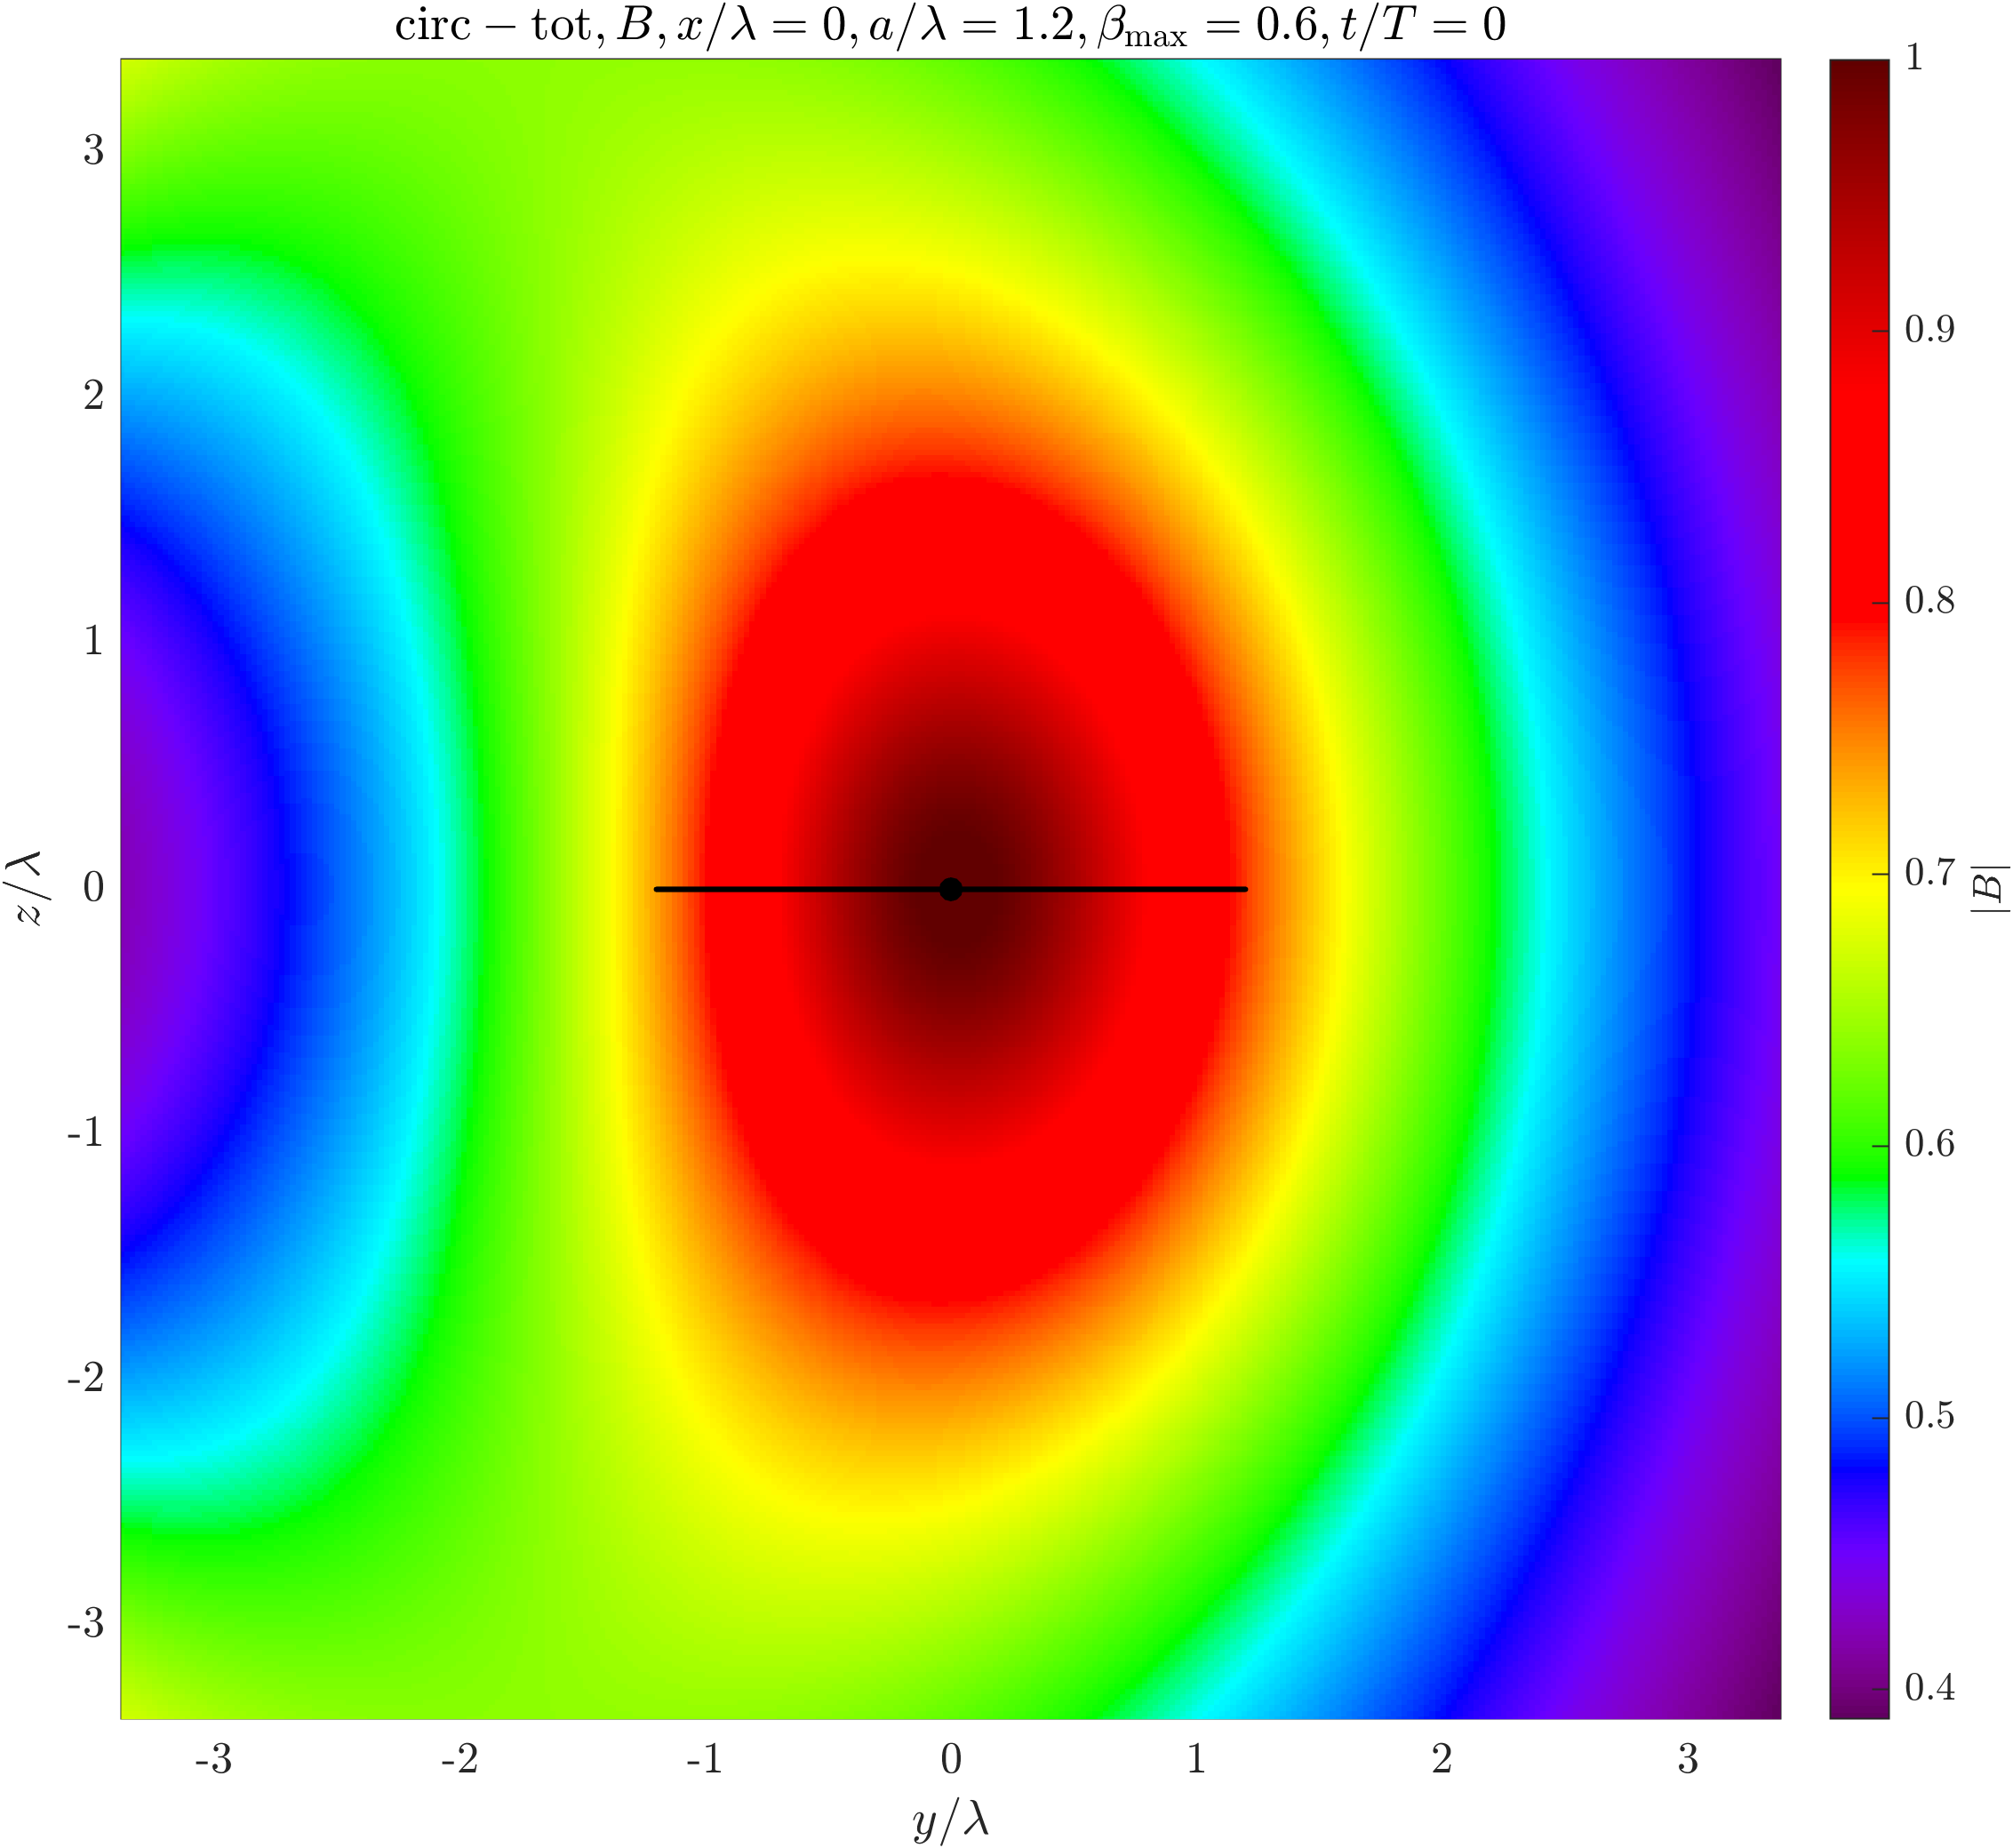
\includegraphics[width=\textwidth]{radiation_fig/circular_motion_b_yz_beta_0_6.png}
		\caption{\(B|_{yz}\) (\(\beta=0.6\))}
		\label{点电荷圆周运动辐射场示意图-B|_yz(beta=0.6)}
	\end{subfigure}
	\vspace{0.2cm}
	\begin{subfigure}[b]{0.23\textwidth}
		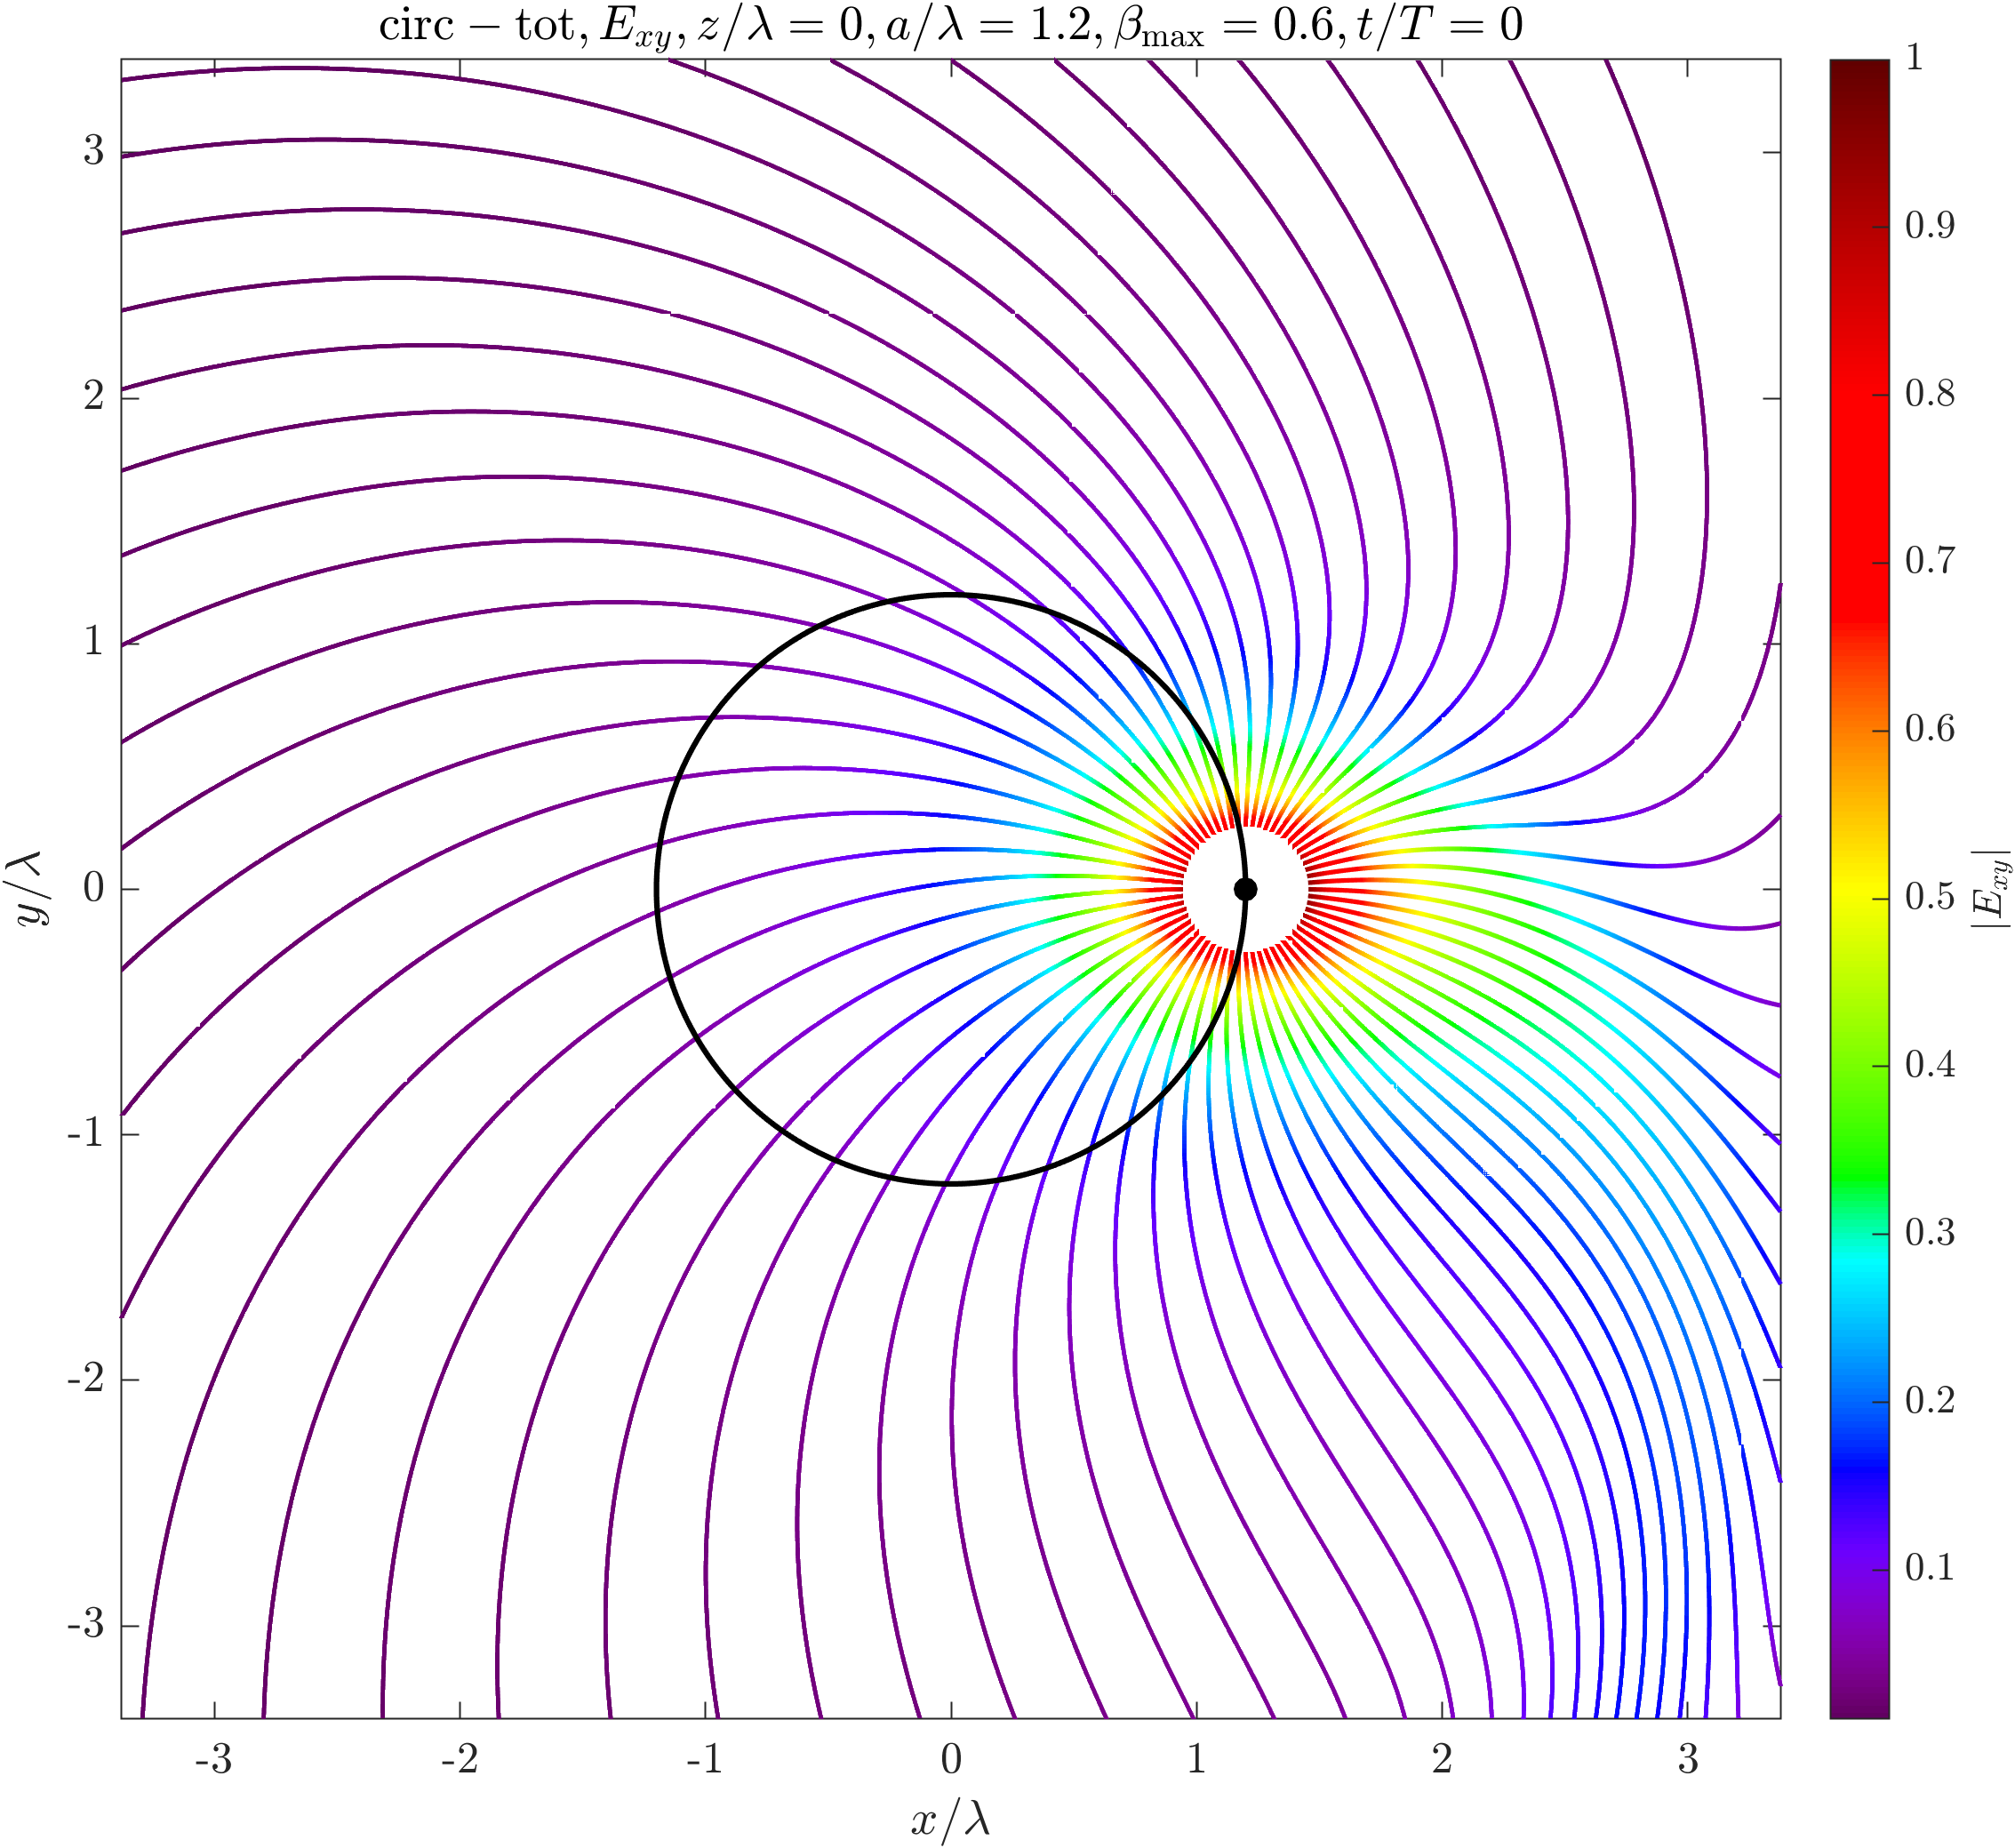
\includegraphics[width=\textwidth]{radiation_fig/circular_motion_e_farfield_xy_beta_0_6.png}
		\caption{\(E|_{xy}\) (\(\beta=0.6\))}
		\label{点电荷圆周运动辐射场示意图-E|_xy(beta=0.6)-2}
	\end{subfigure}
	\hfill
	\begin{subfigure}[b]{0.23\textwidth}
		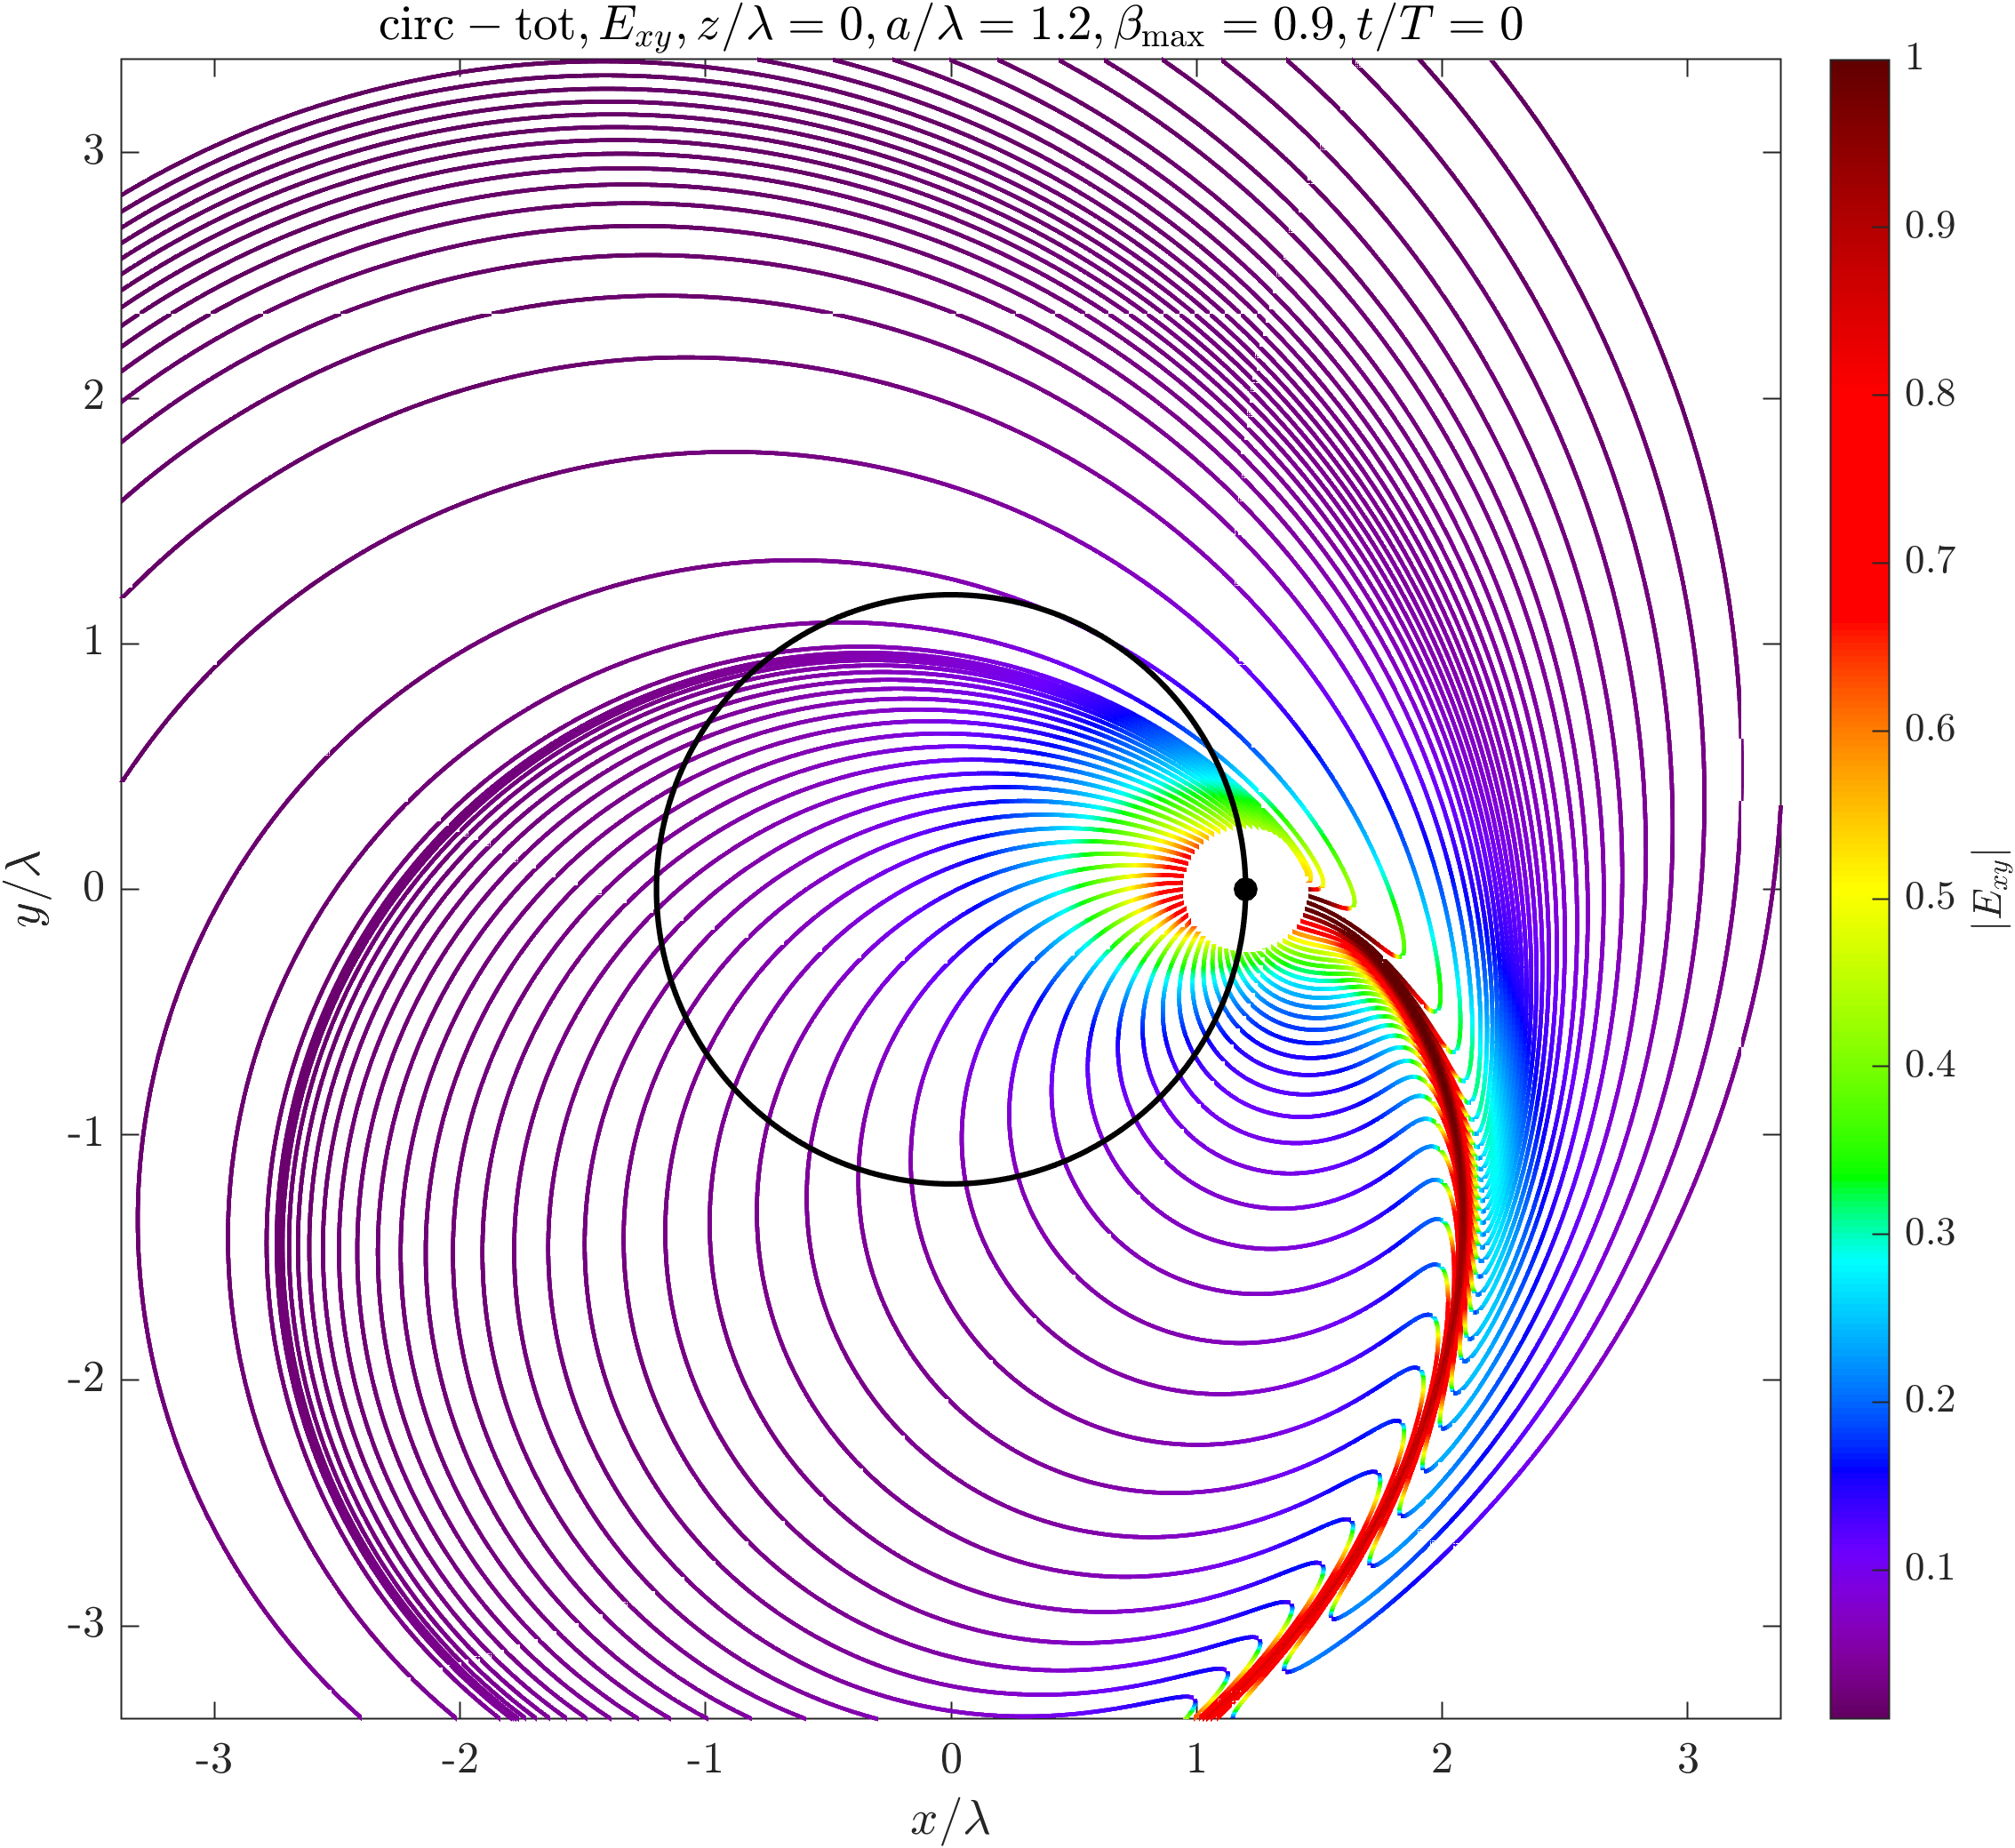
\includegraphics[width=\textwidth]{radiation_fig/circular_motion_e_farfield_xy_beta_0_9.png}
		\caption{\(E|_{xy}\) (\(\beta=0.9\))}
		\label{点电荷圆周运动辐射场示意图-E|_xy(beta=0.9)-2}
	\end{subfigure}
	\hfill
	\begin{subfigure}[b]{0.23\textwidth}
		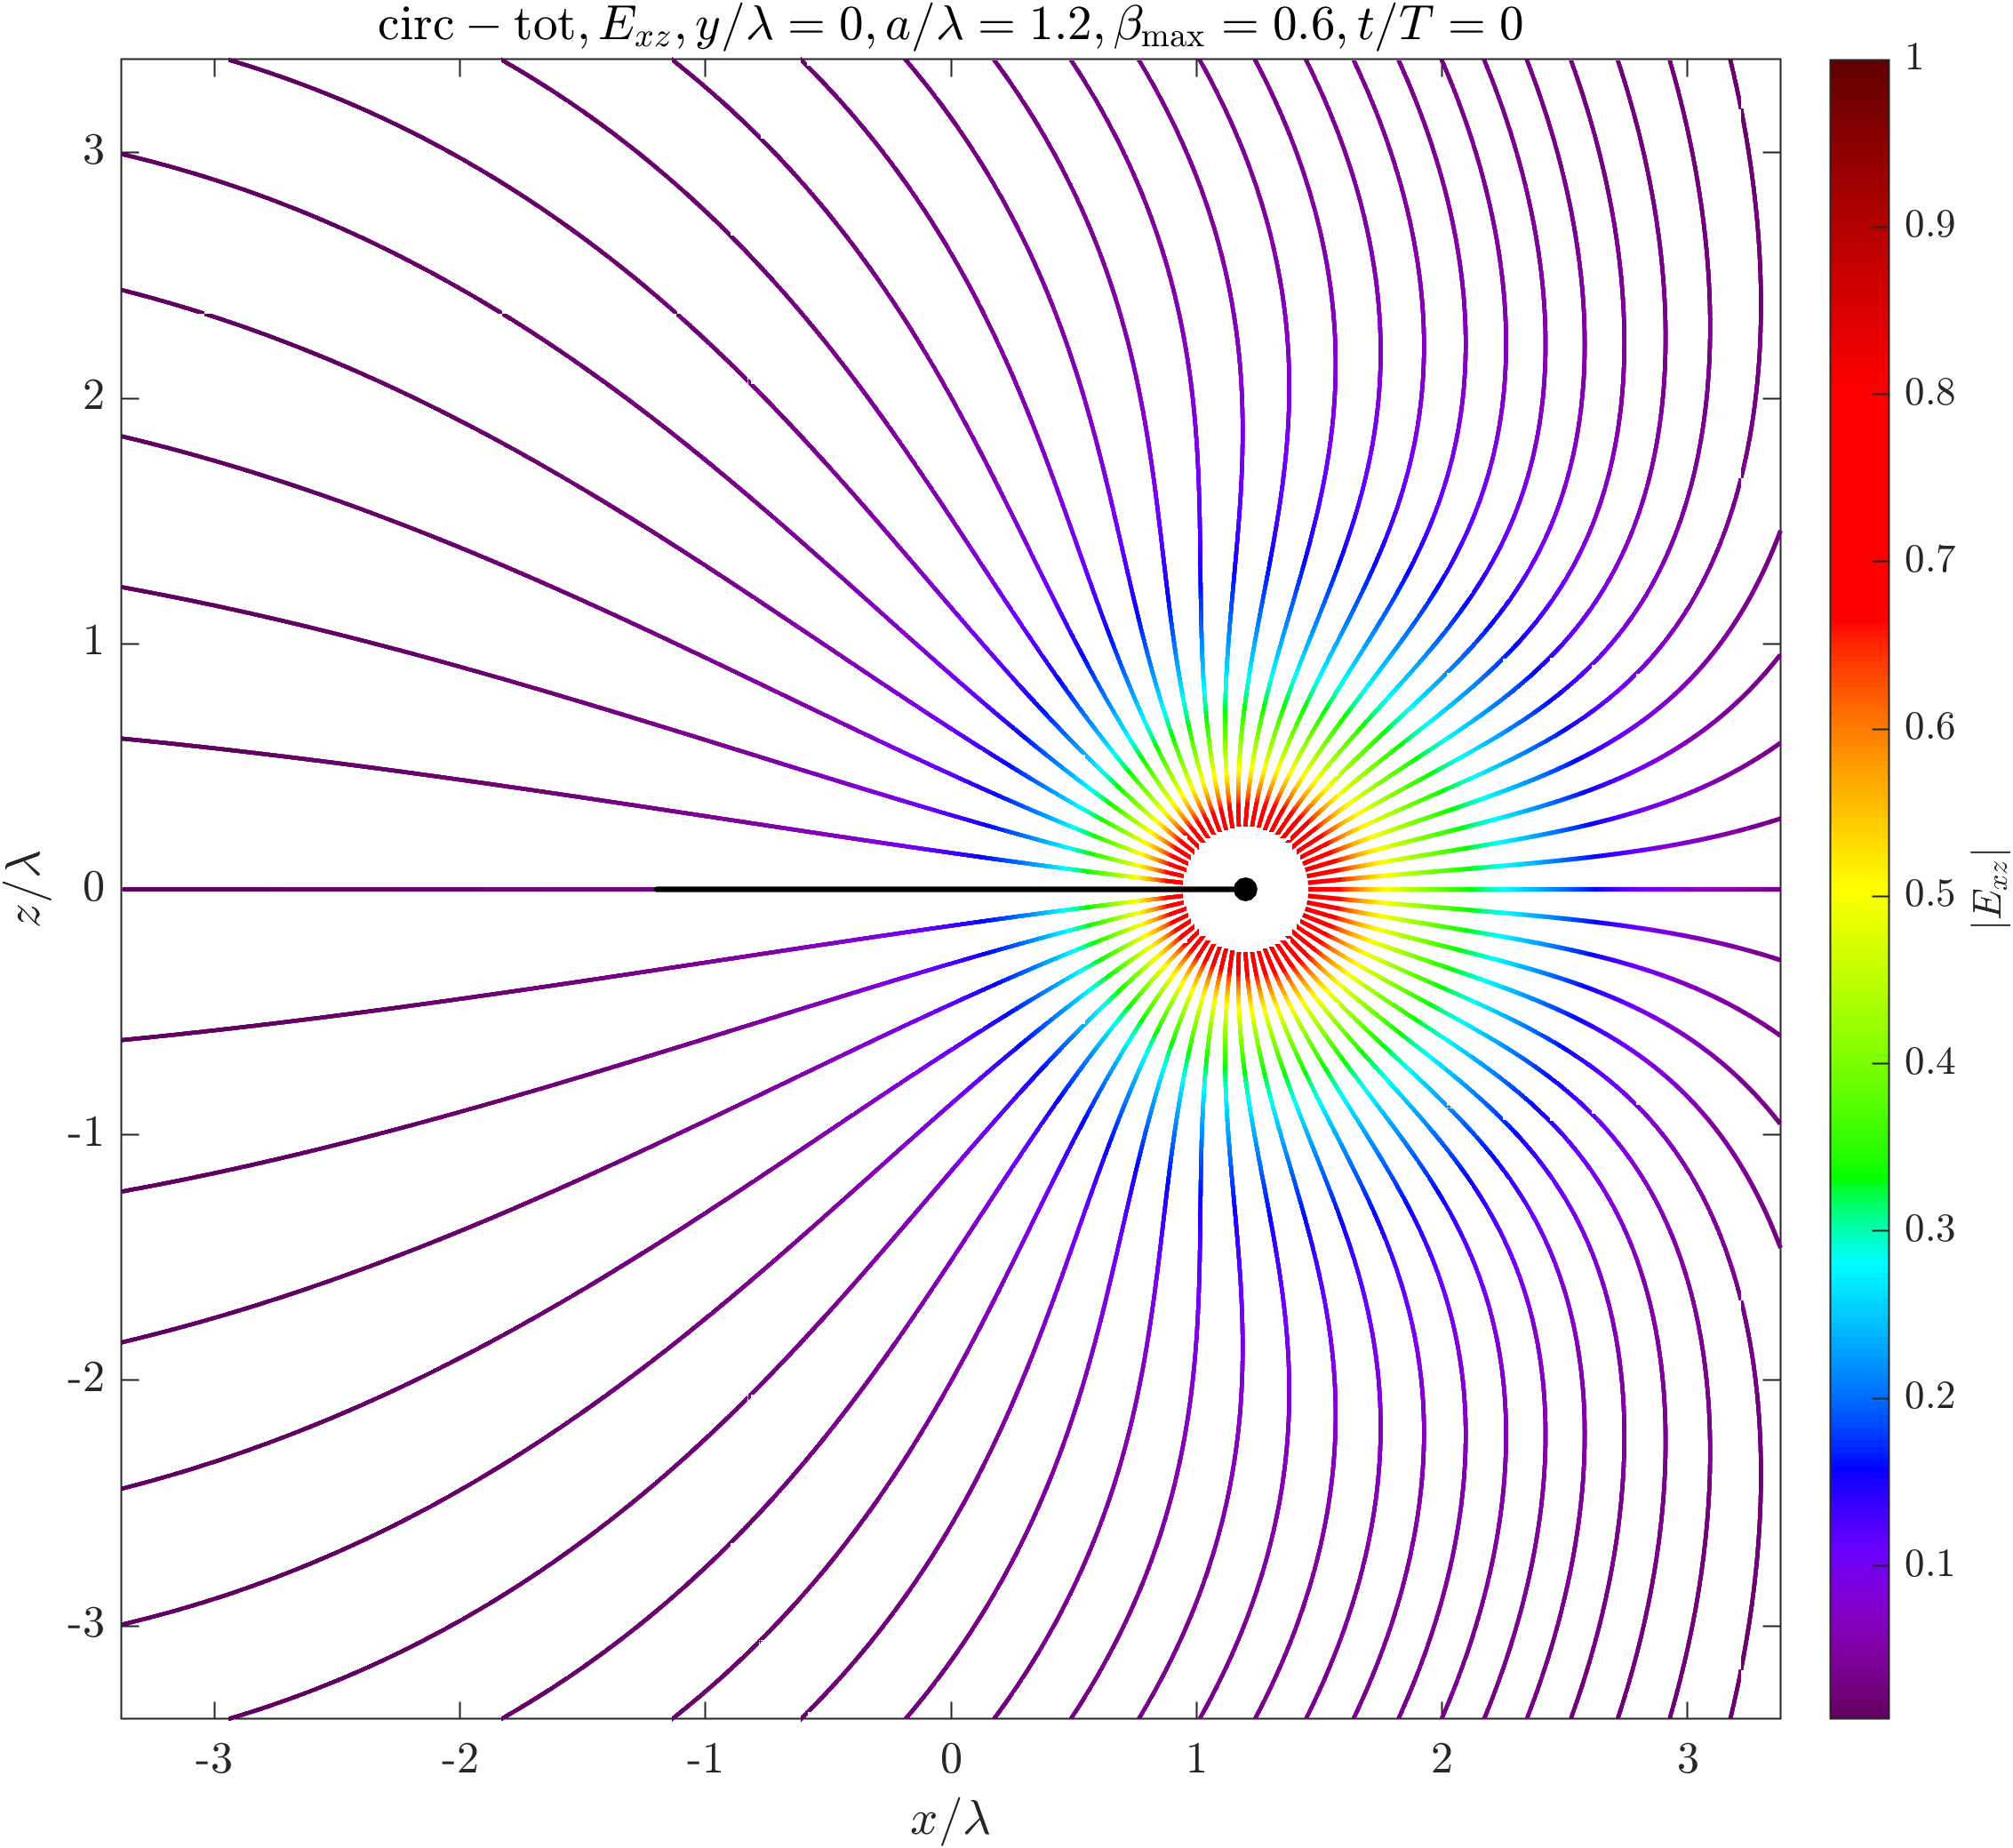
\includegraphics[width=\textwidth]{radiation_fig/circular_motion_e_farfield_xz_beta_0_6.png}
		\caption{\(E|_{xz}\) (\(\beta=0.6\))}
		\label{点电荷圆周运动辐射场示意图-E|_xz(beta=0.6)-2}
	\end{subfigure}
	\hfill
	\begin{subfigure}[b]{0.23\textwidth}
		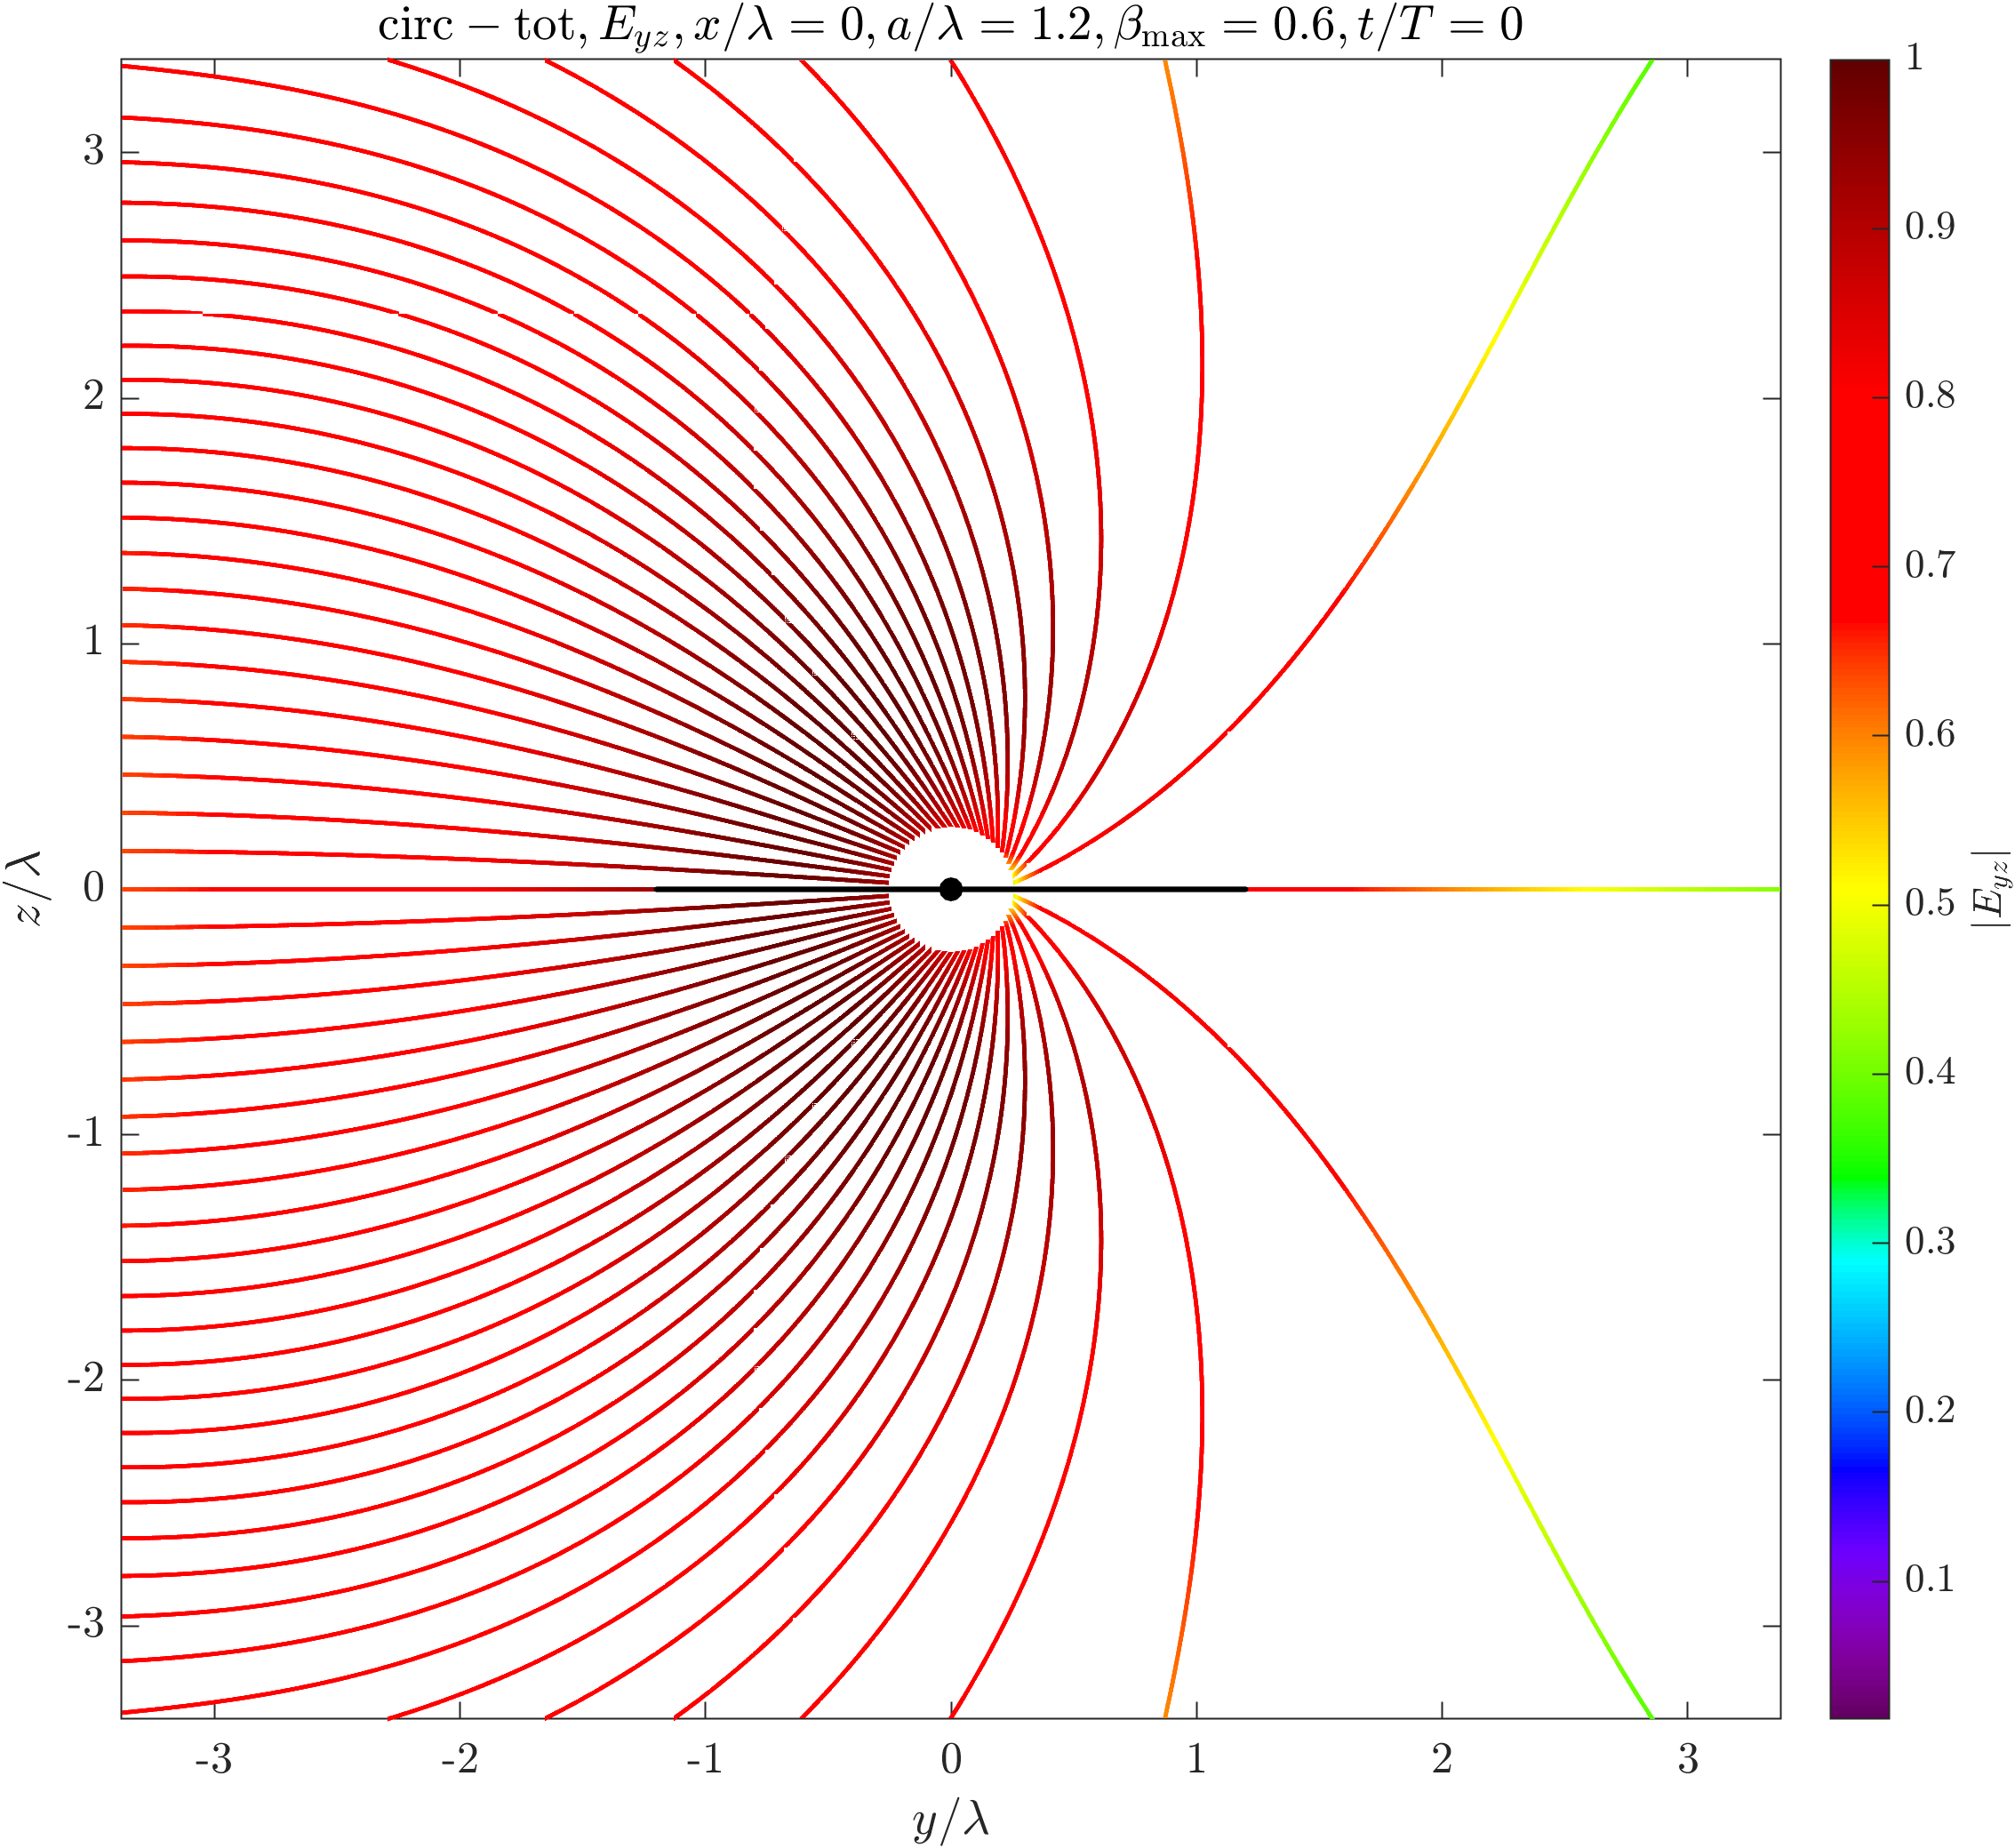
\includegraphics[width=\textwidth]{radiation_fig/circular_motion_e_farfield_yz_beta_0_6.png}
		\caption{\(E|_{yz}\) (\(\beta=0.6\))}
		\label{点电荷圆周运动辐射场示意图-E|_yz(beta=0.6)-2}
	\end{subfigure}
	\vspace{0.2cm}
	\begin{subfigure}[b]{0.23\textwidth}
		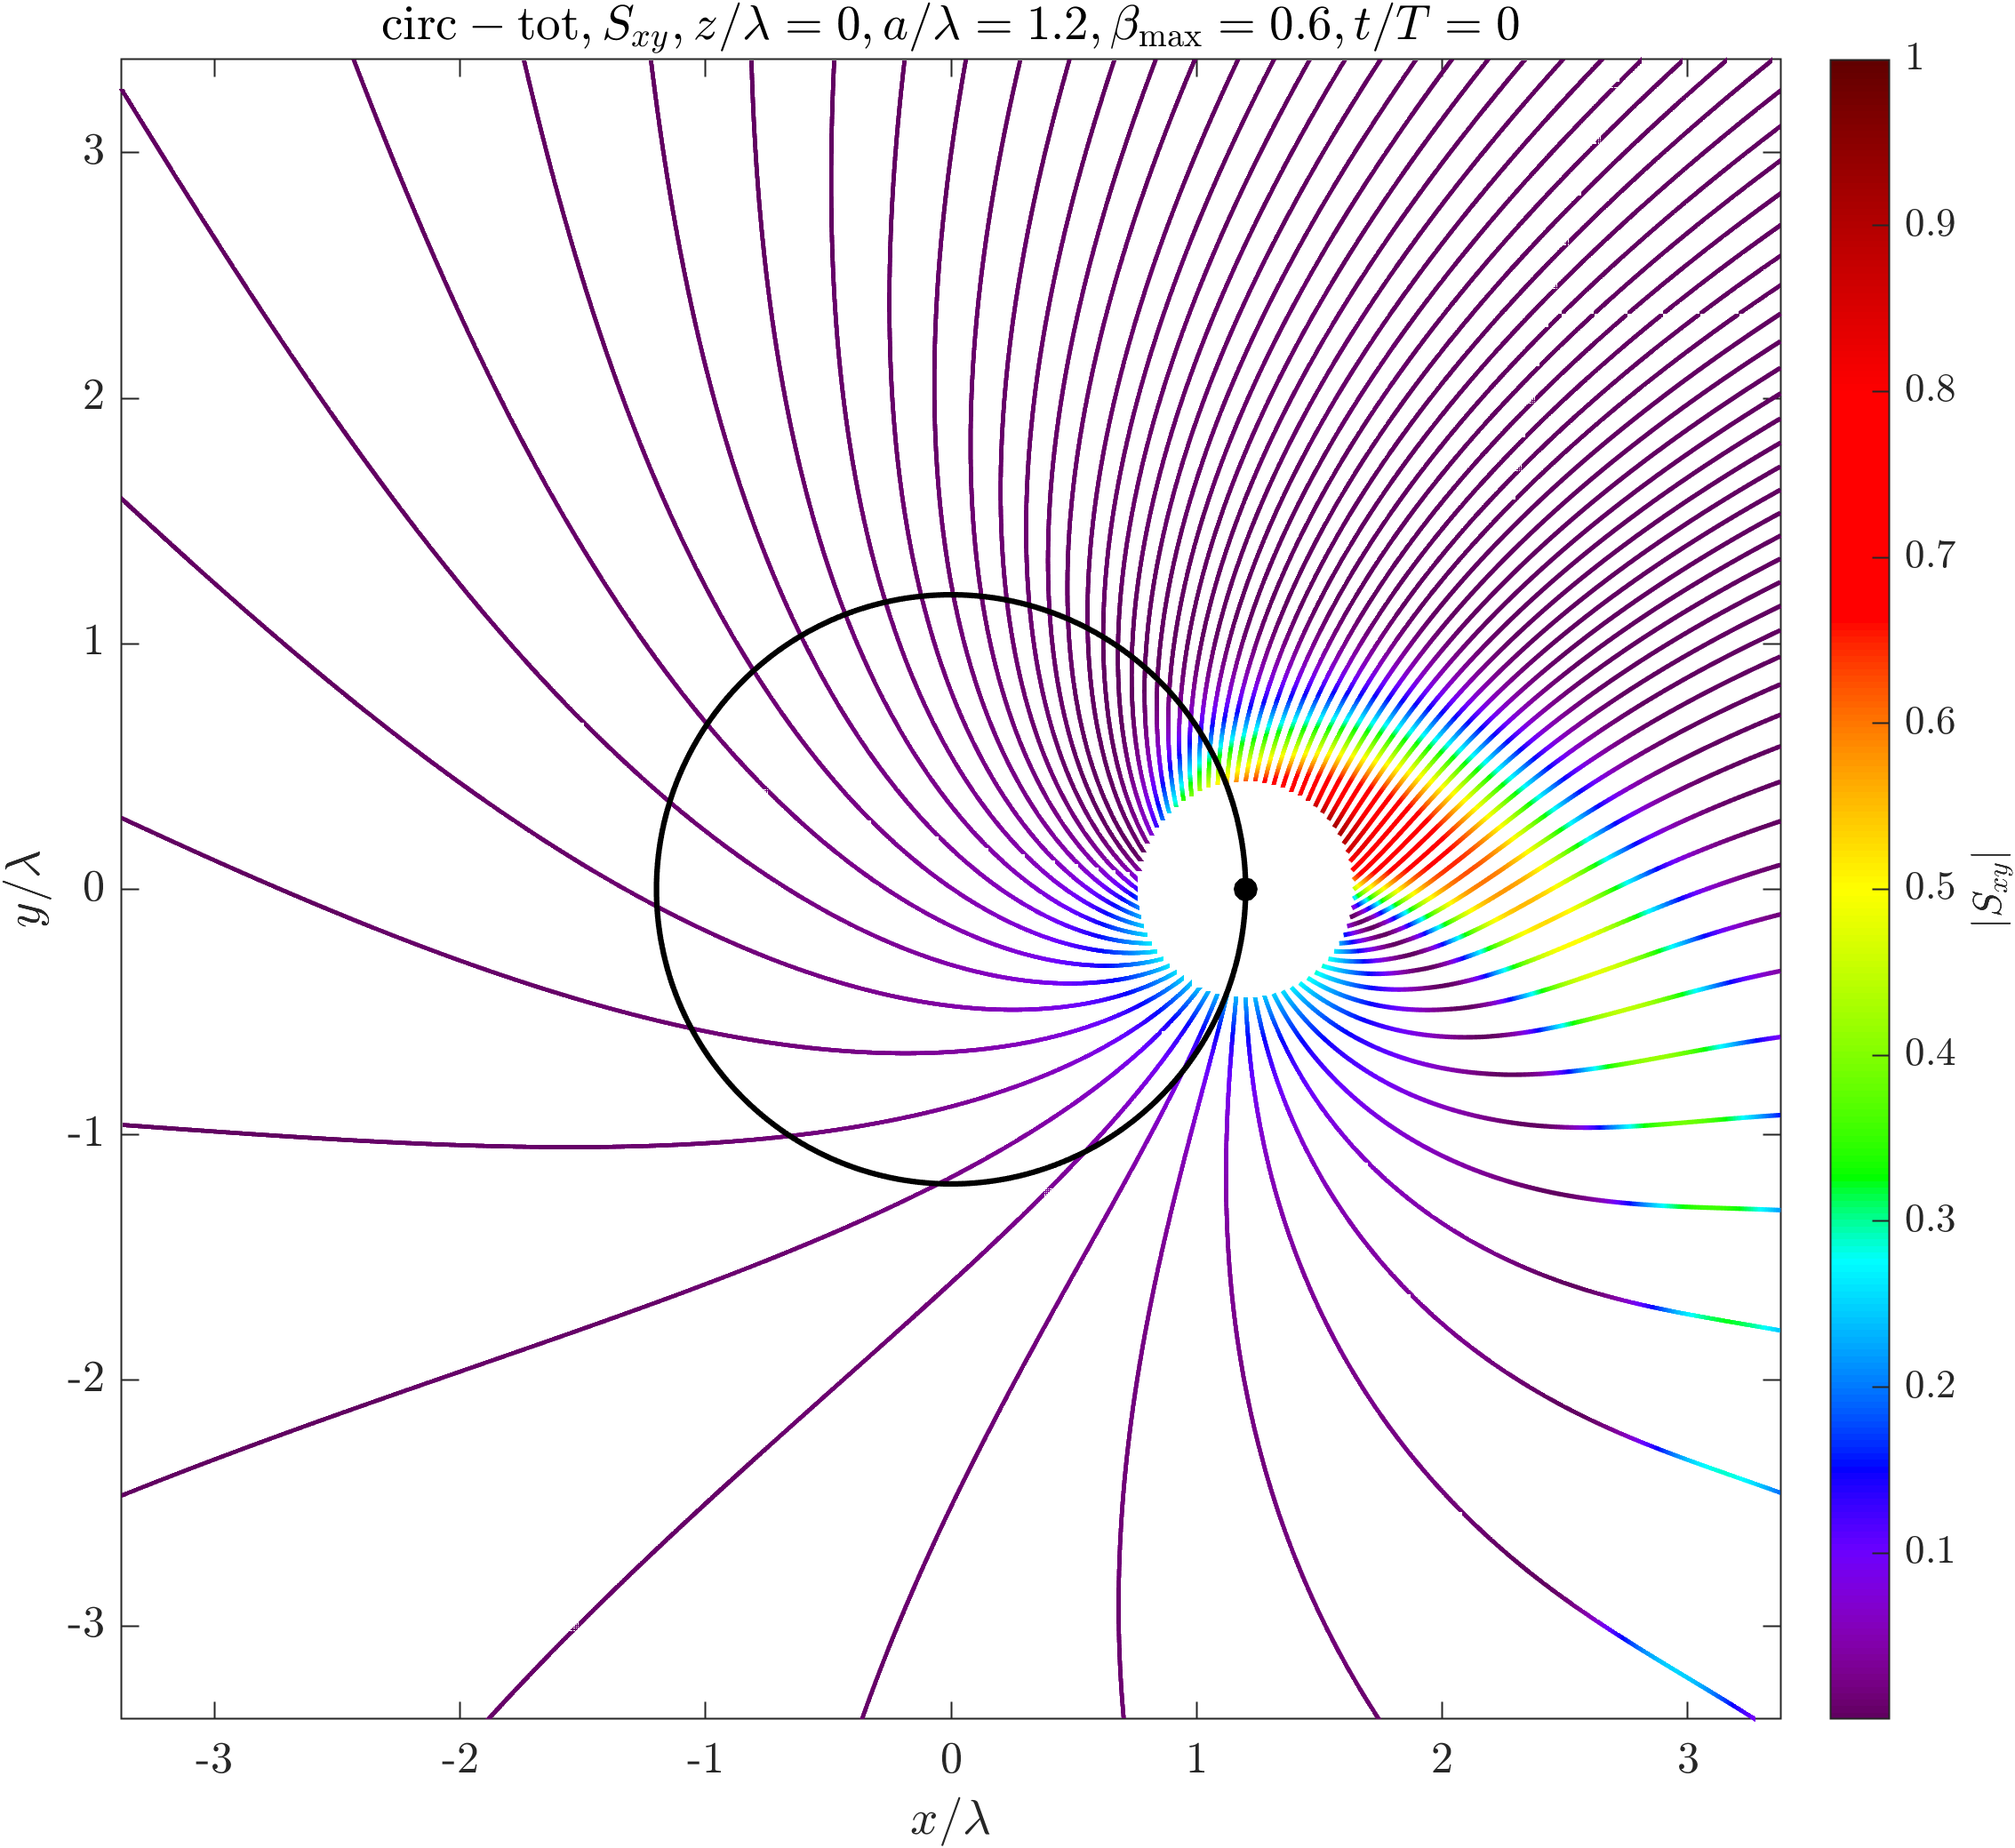
\includegraphics[width=\textwidth]{radiation_fig/circular_motion_s_xy_beta_0_6.png}
		\caption{\(S|_{xy}\) (\(\beta=0.6\))}
		\label{点电荷圆周运动辐射场示意图-S|_xy(beta=0.6)}
	\end{subfigure}
	\hfill
	\begin{subfigure}[b]{0.23\textwidth}
		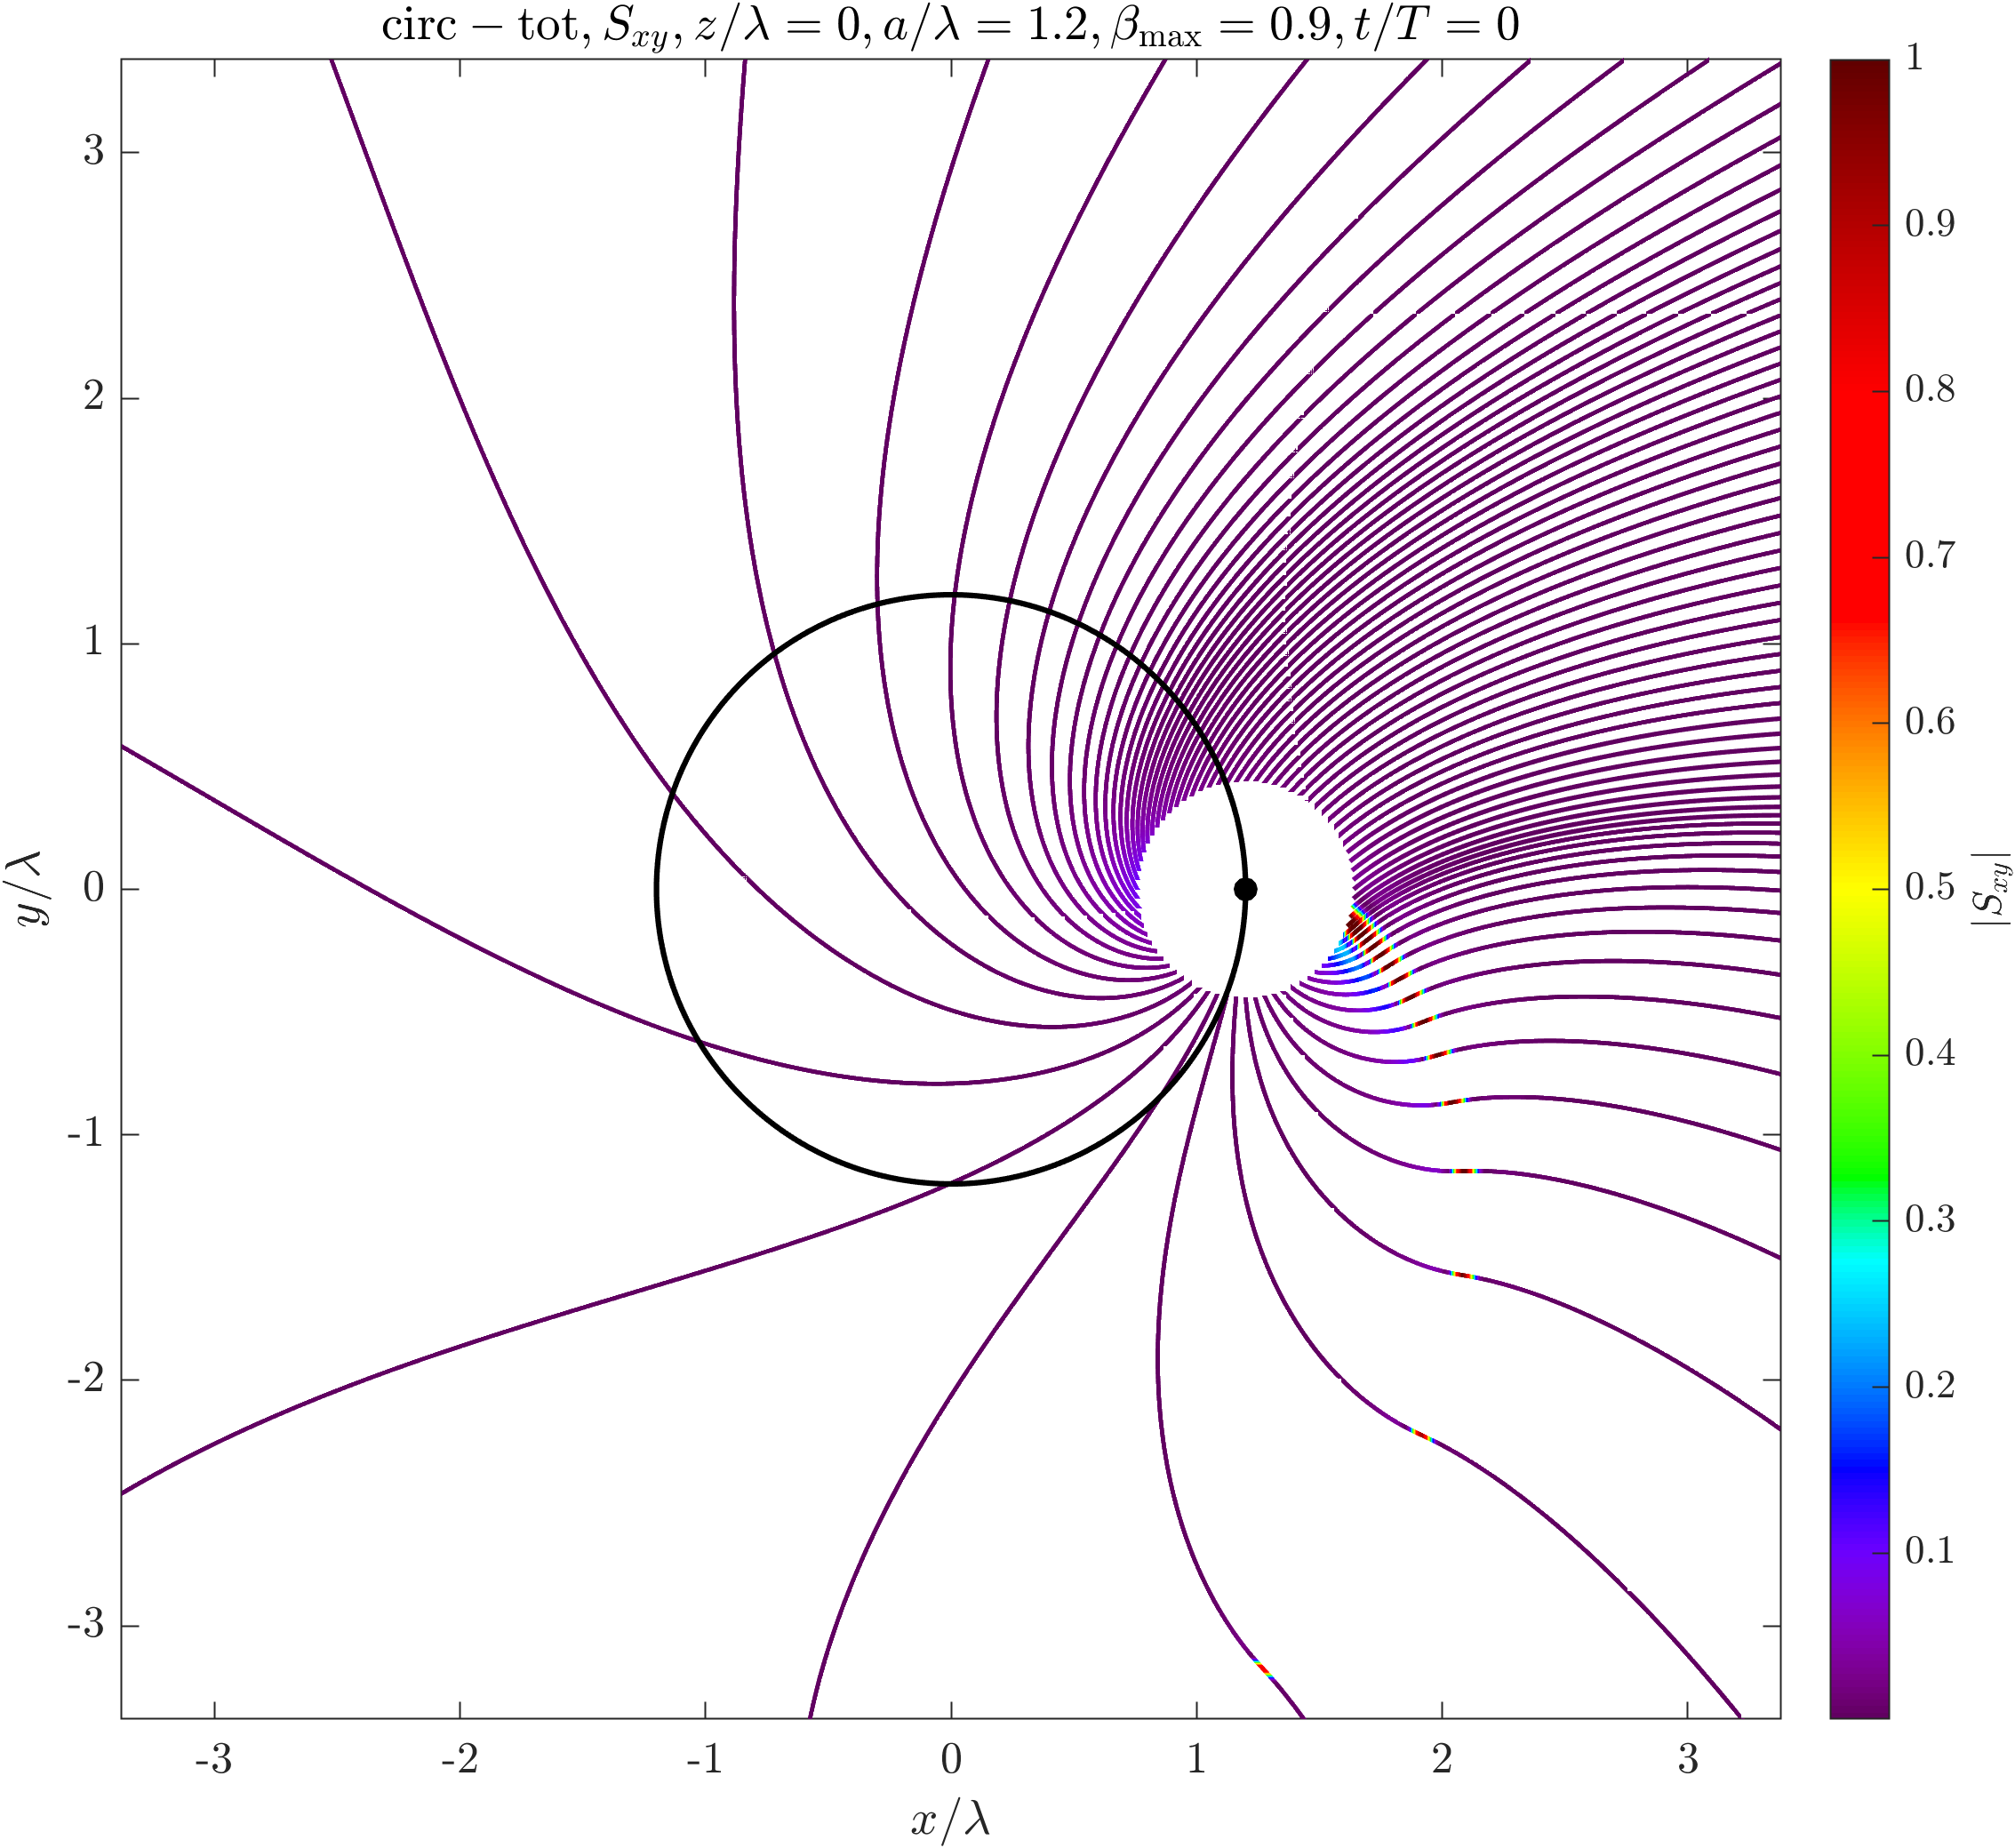
\includegraphics[width=\textwidth]{radiation_fig/circular_motion_s_xy_beta_0_9.png}
		\caption{\(S|_{xy}\) (\(\beta=0.9\))}
		\label{点电荷圆周运动辐射场示意图-S|_xy(beta=0.9)}
	\end{subfigure}
	\hfill
	\begin{subfigure}[b]{0.23\textwidth}
		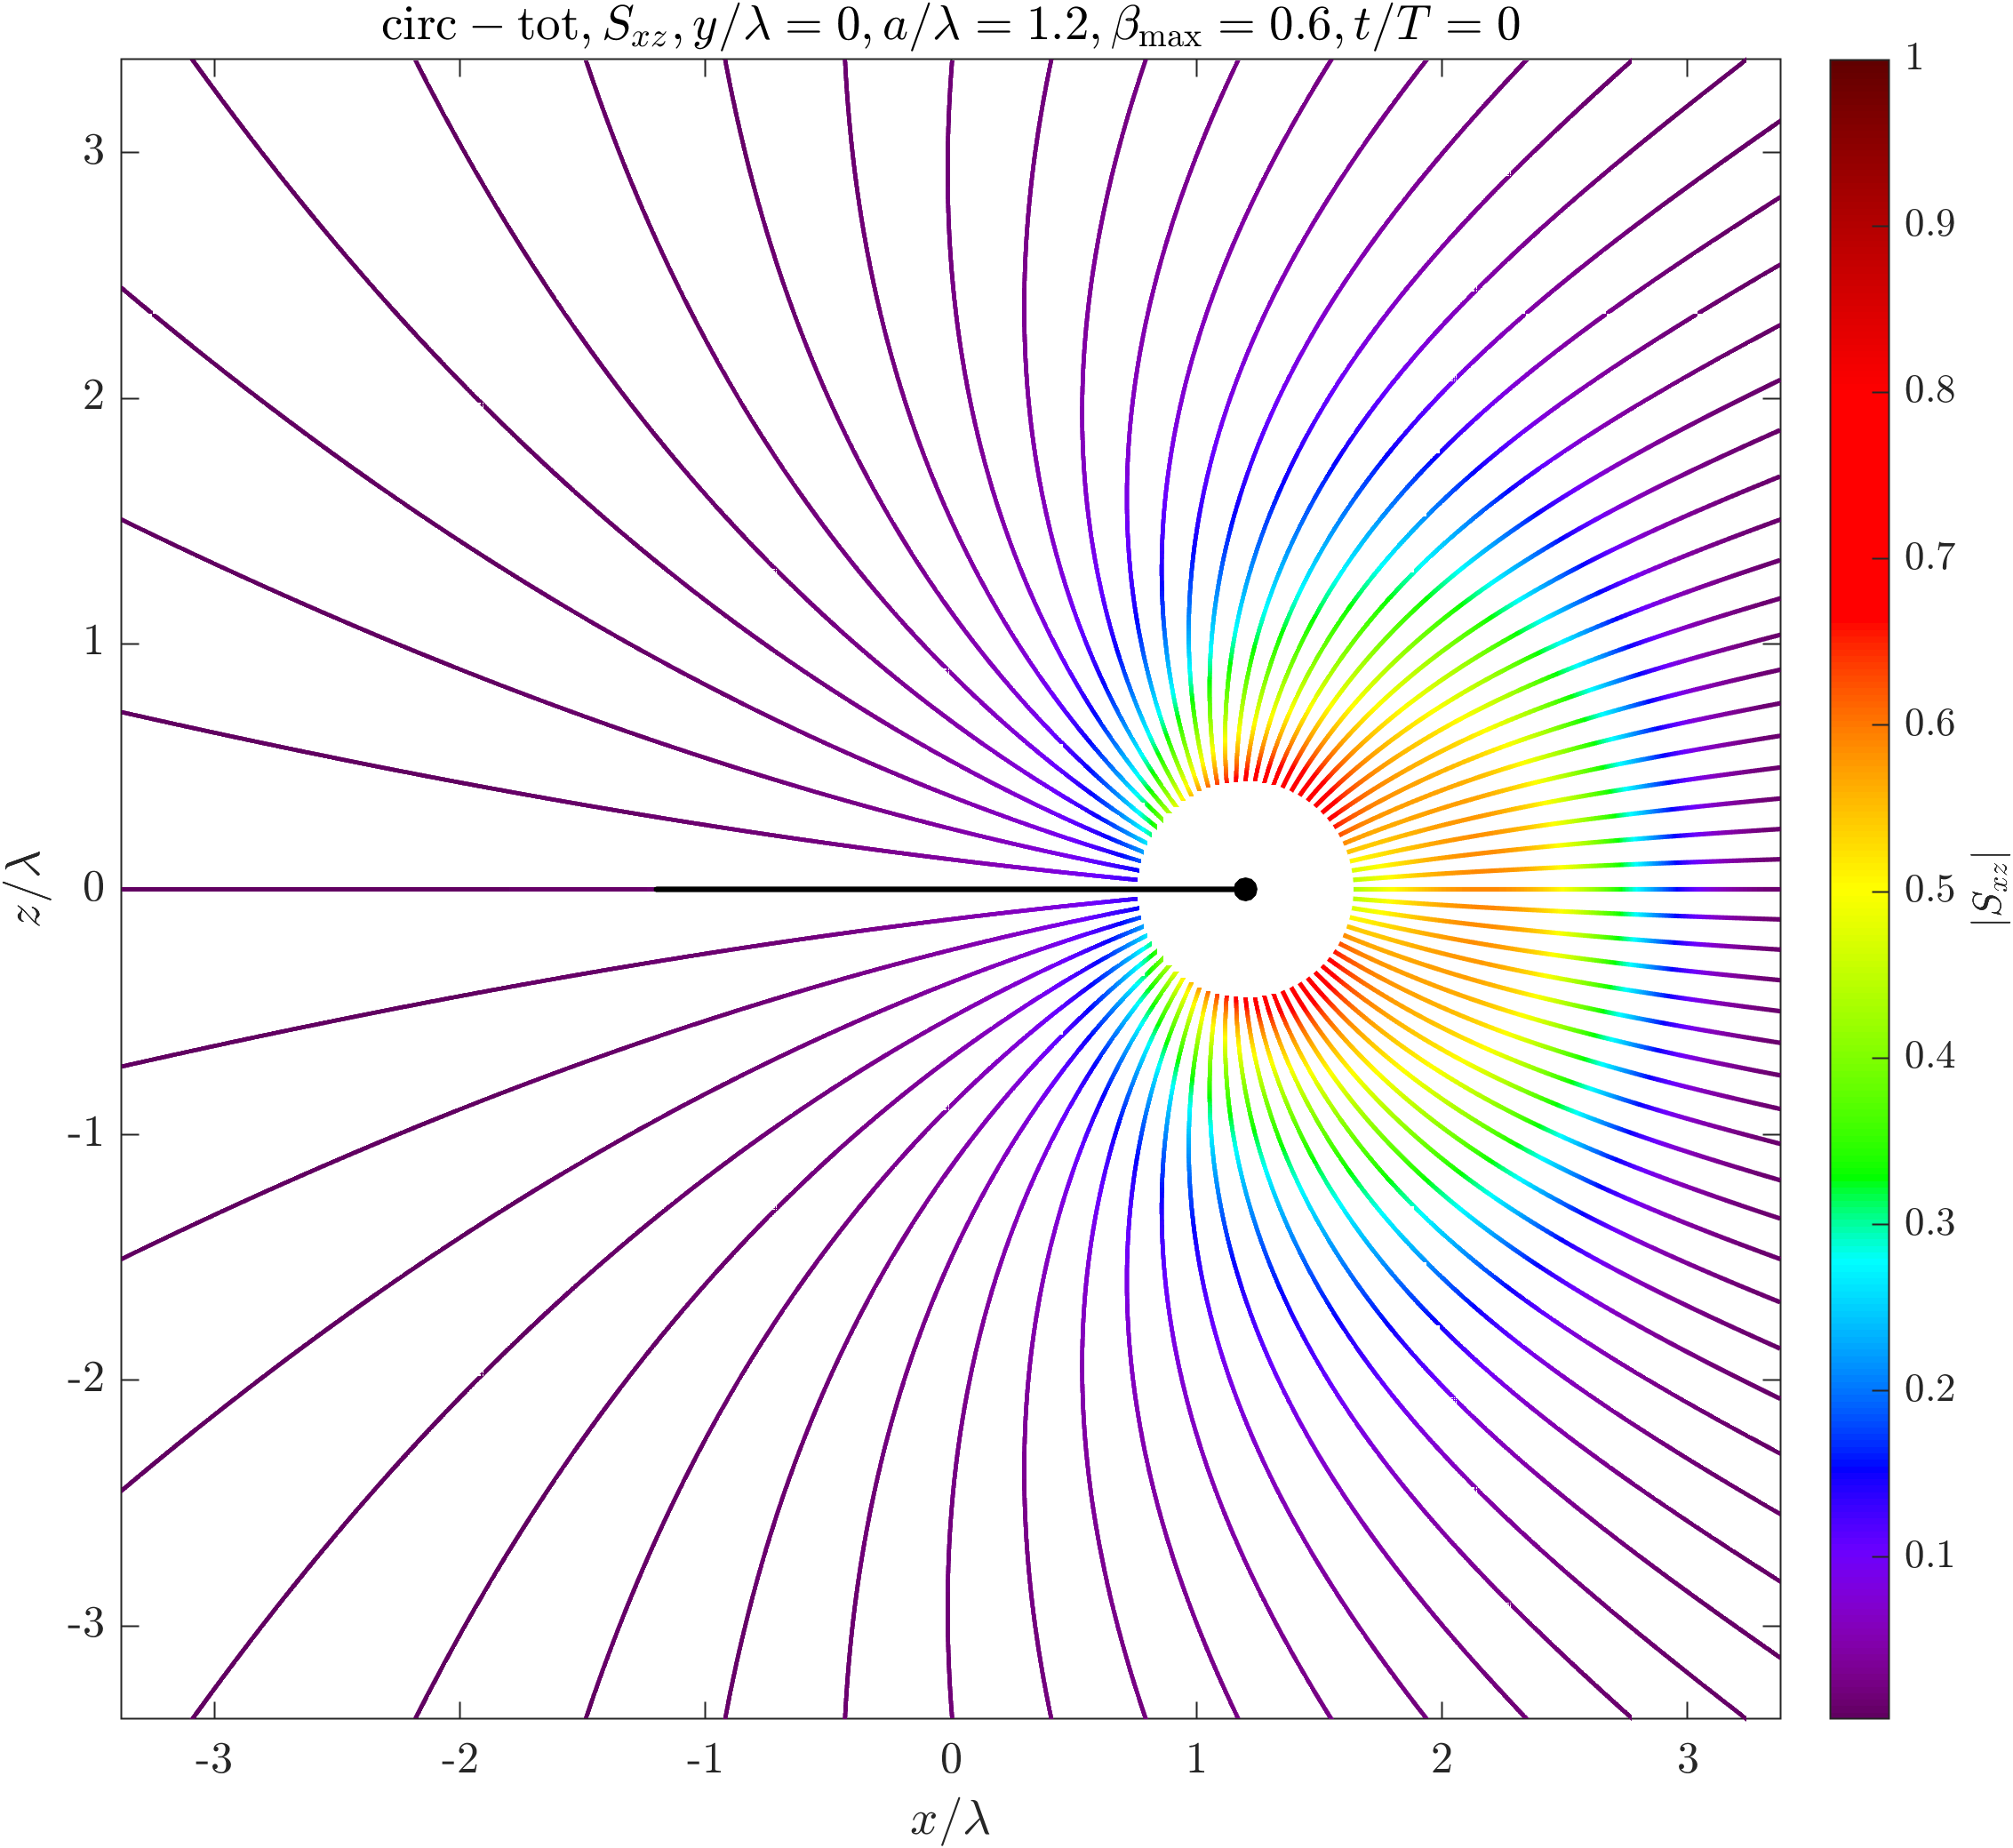
\includegraphics[width=\textwidth]{radiation_fig/circular_motion_s_xz_beta_0_6.png}
		\caption{\(S|_{xz}\) (\(\beta=0.6\))}
		\label{点电荷圆周运动辐射场示意图-S|_xz(beta=0.6)}
	\end{subfigure}
	\hfill
	\begin{subfigure}[b]{0.23\textwidth}
		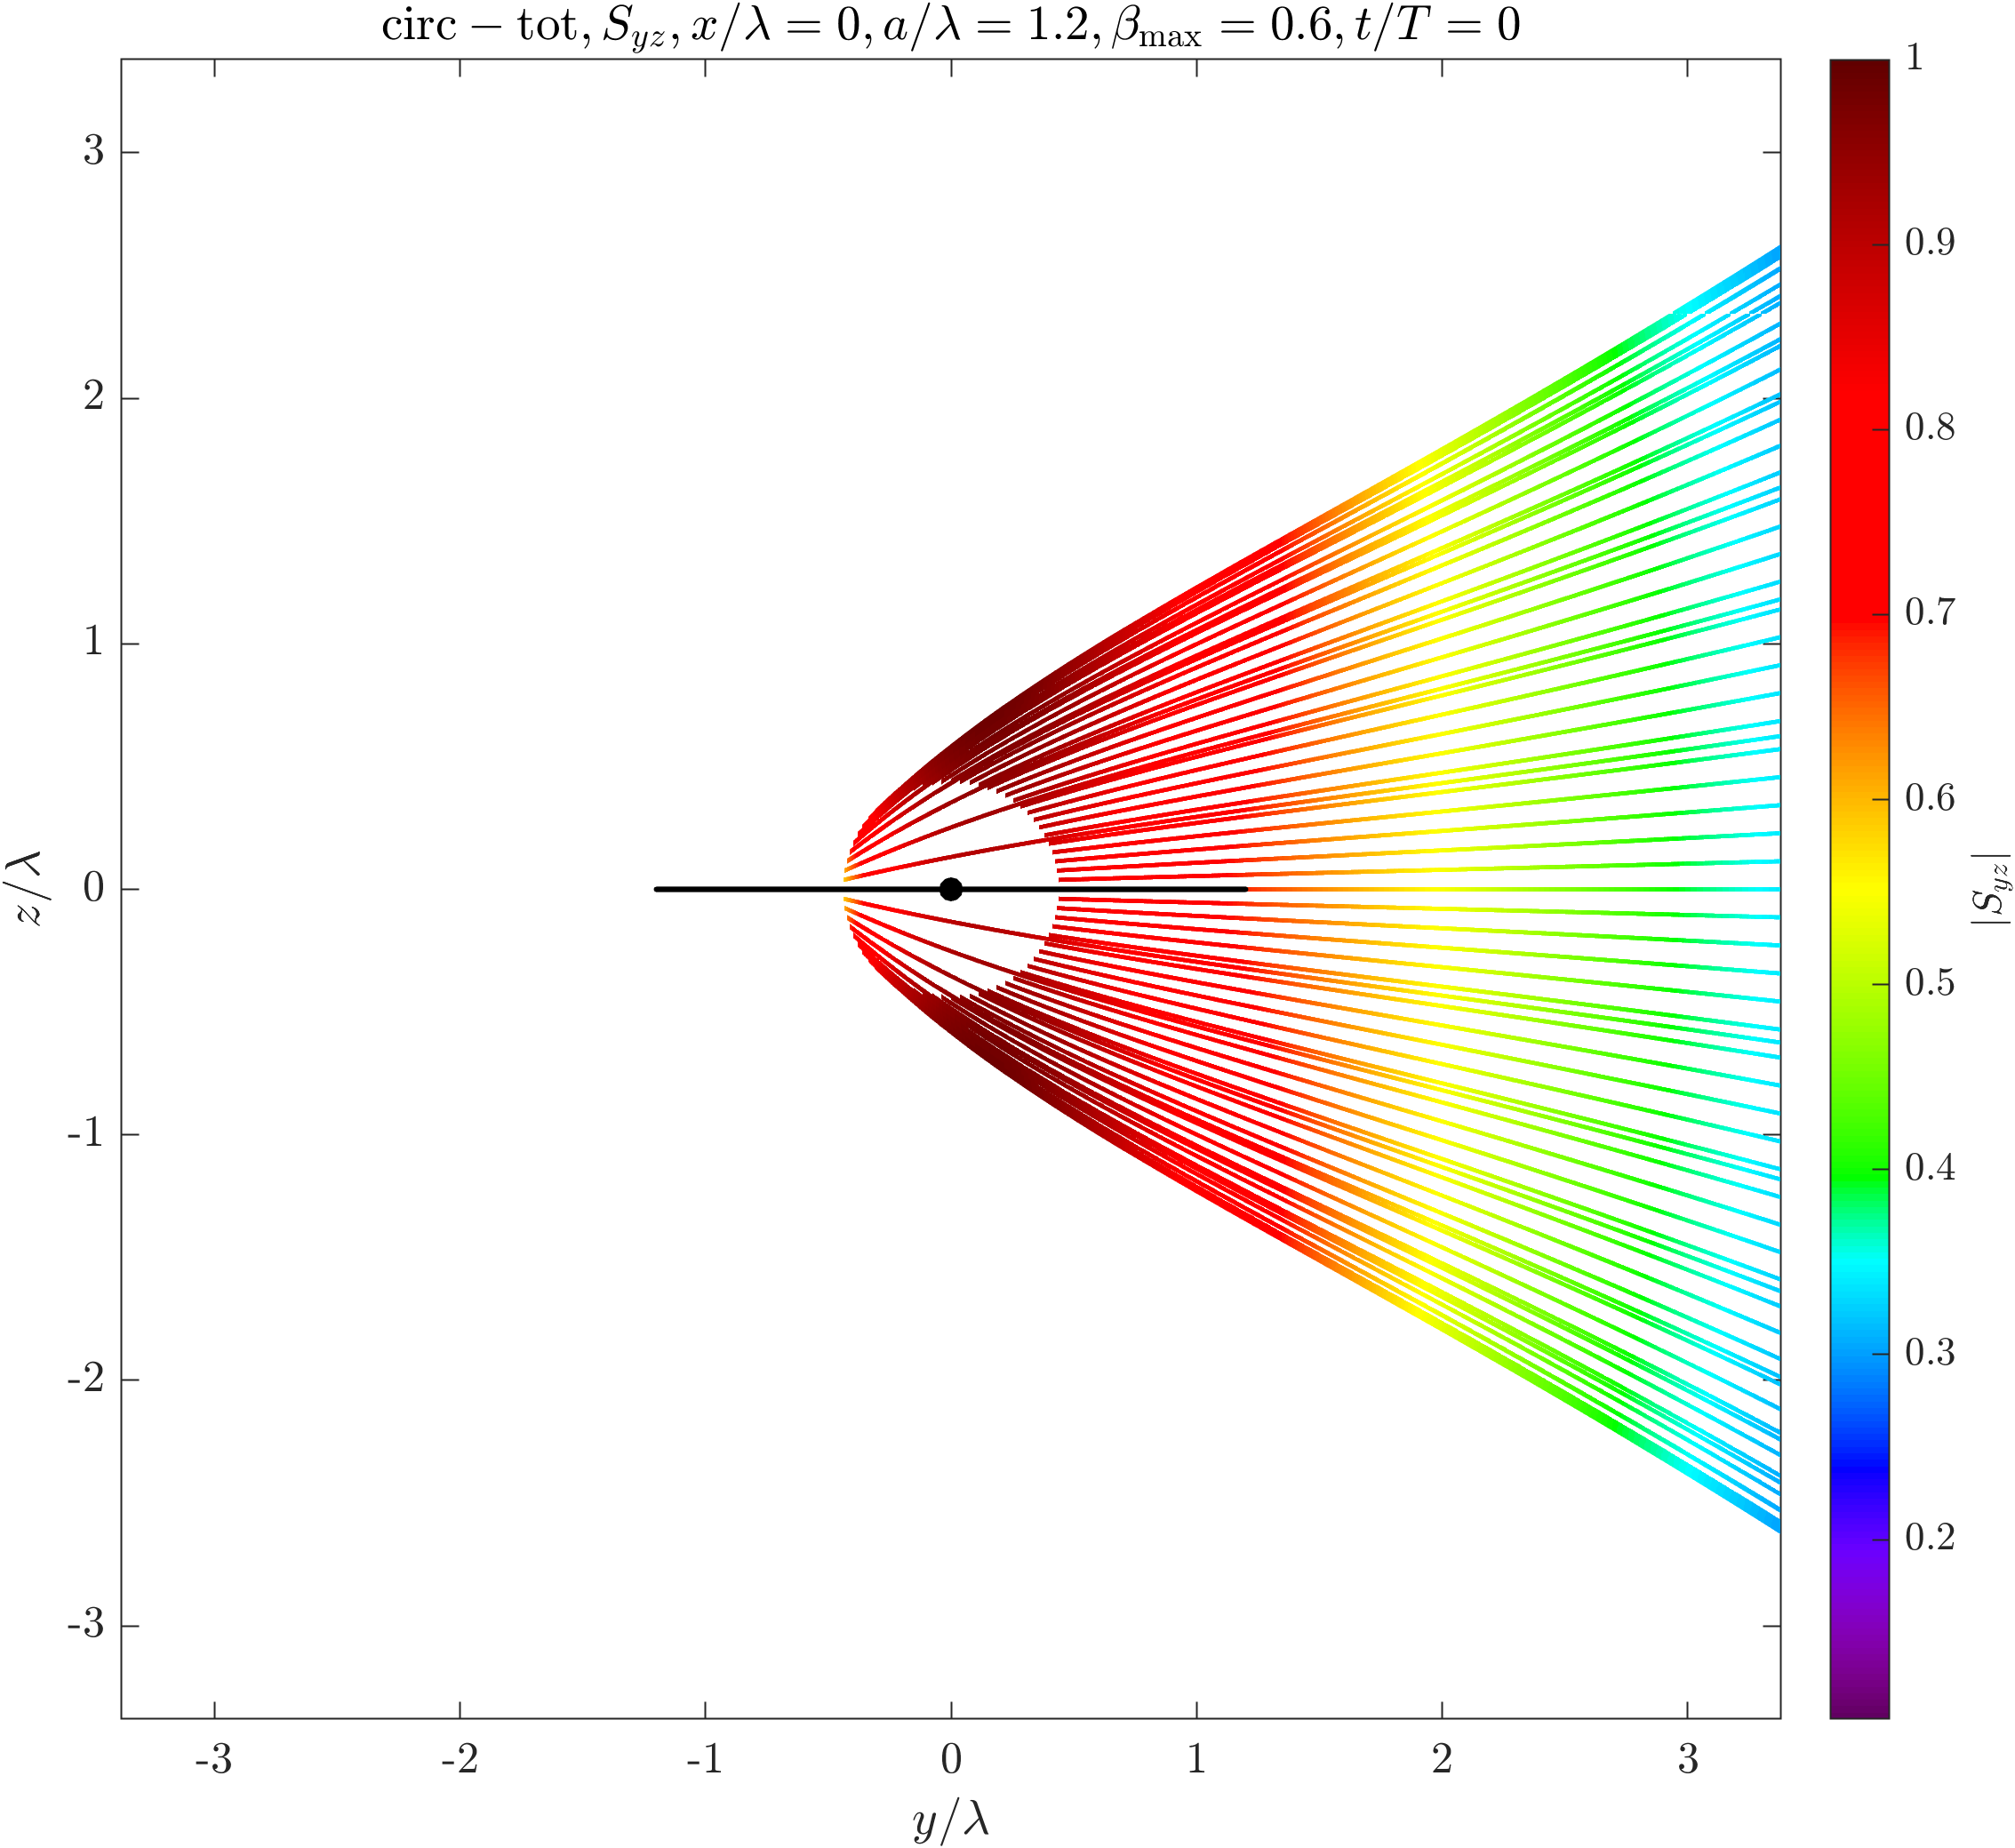
\includegraphics[width=\textwidth]{radiation_fig/circular_motion_s_yz_beta_0_6.png}
		\caption{\(S|_{yz}\) (\(\beta=0.6\))}
		\label{点电荷圆周运动辐射场示意图-S|_yz(beta=0.6)}
	\end{subfigure}
	\vspace{0.2cm}
	\begin{subfigure}[b]{0.23\textwidth}
		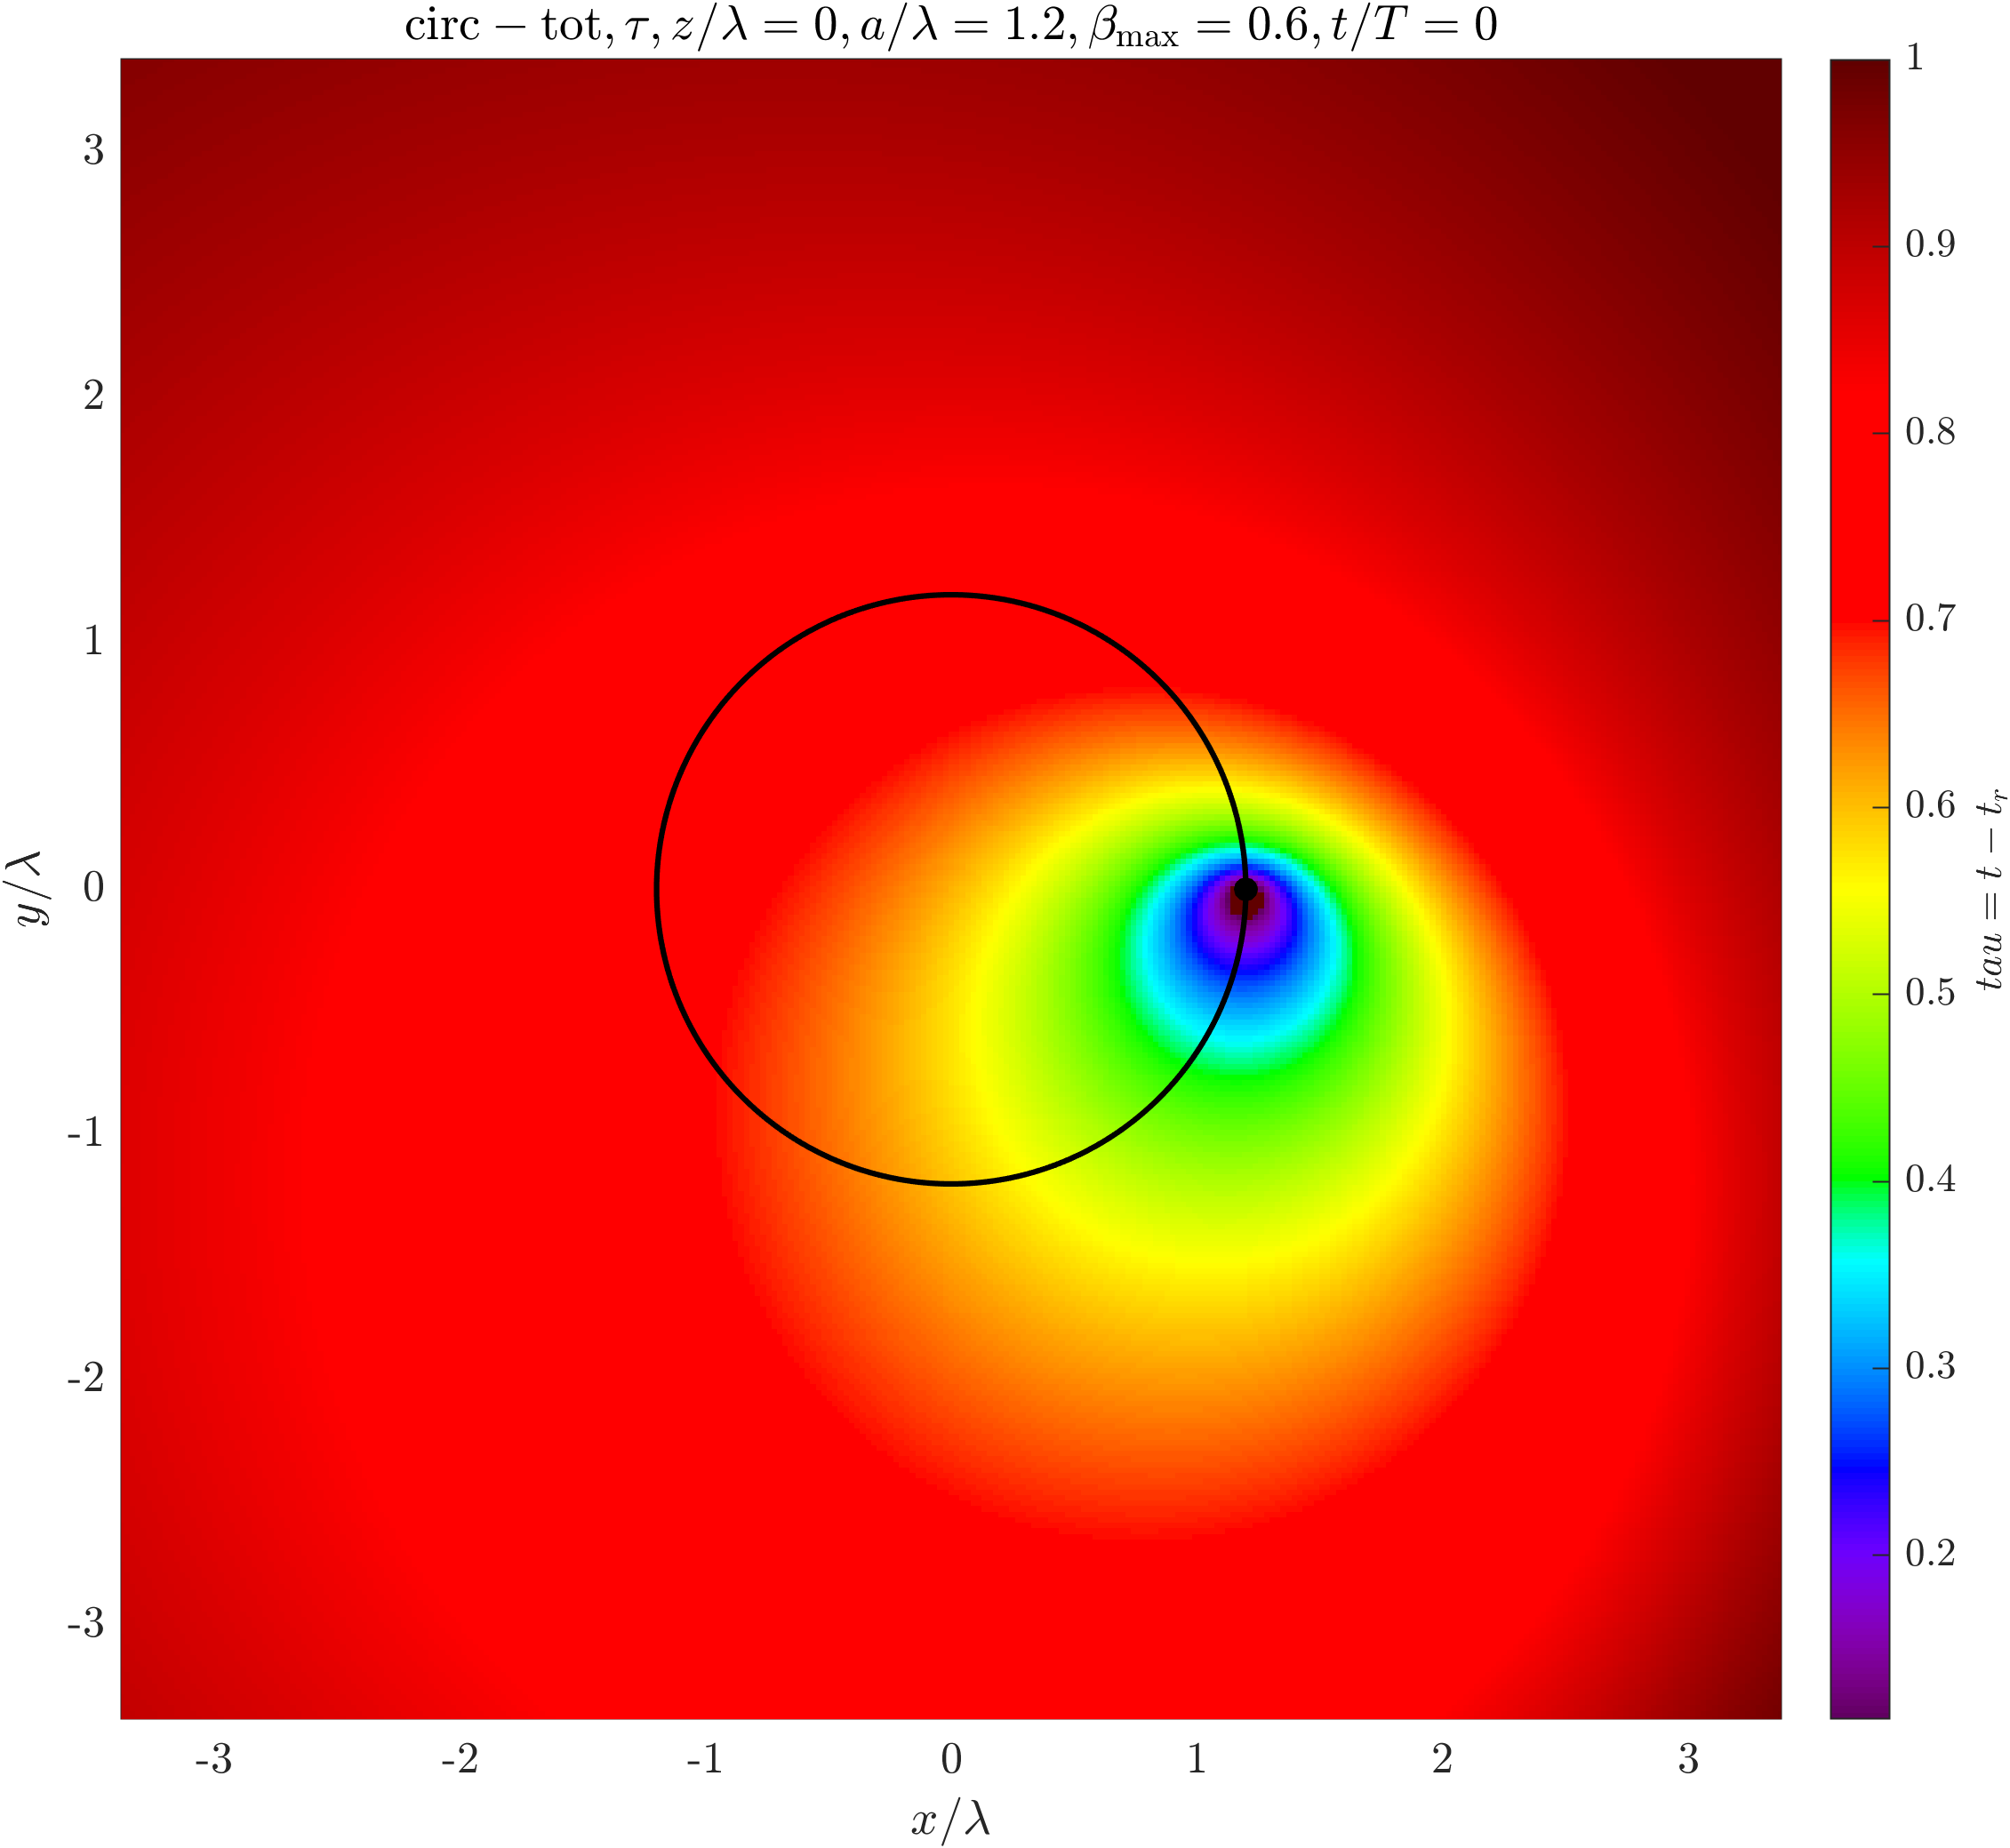
\includegraphics[width=\textwidth]{radiation_fig/circular_motion_tau_xy_beta_0_6.png}
		\caption{\(\tau|_{xy}\) (\(\beta=0.6\))}
		\label{点电荷圆周运动辐射场示意图-tau|_xy(beta=0.6)}
	\end{subfigure}
	\hfill
	\begin{subfigure}[b]{0.23\textwidth}
		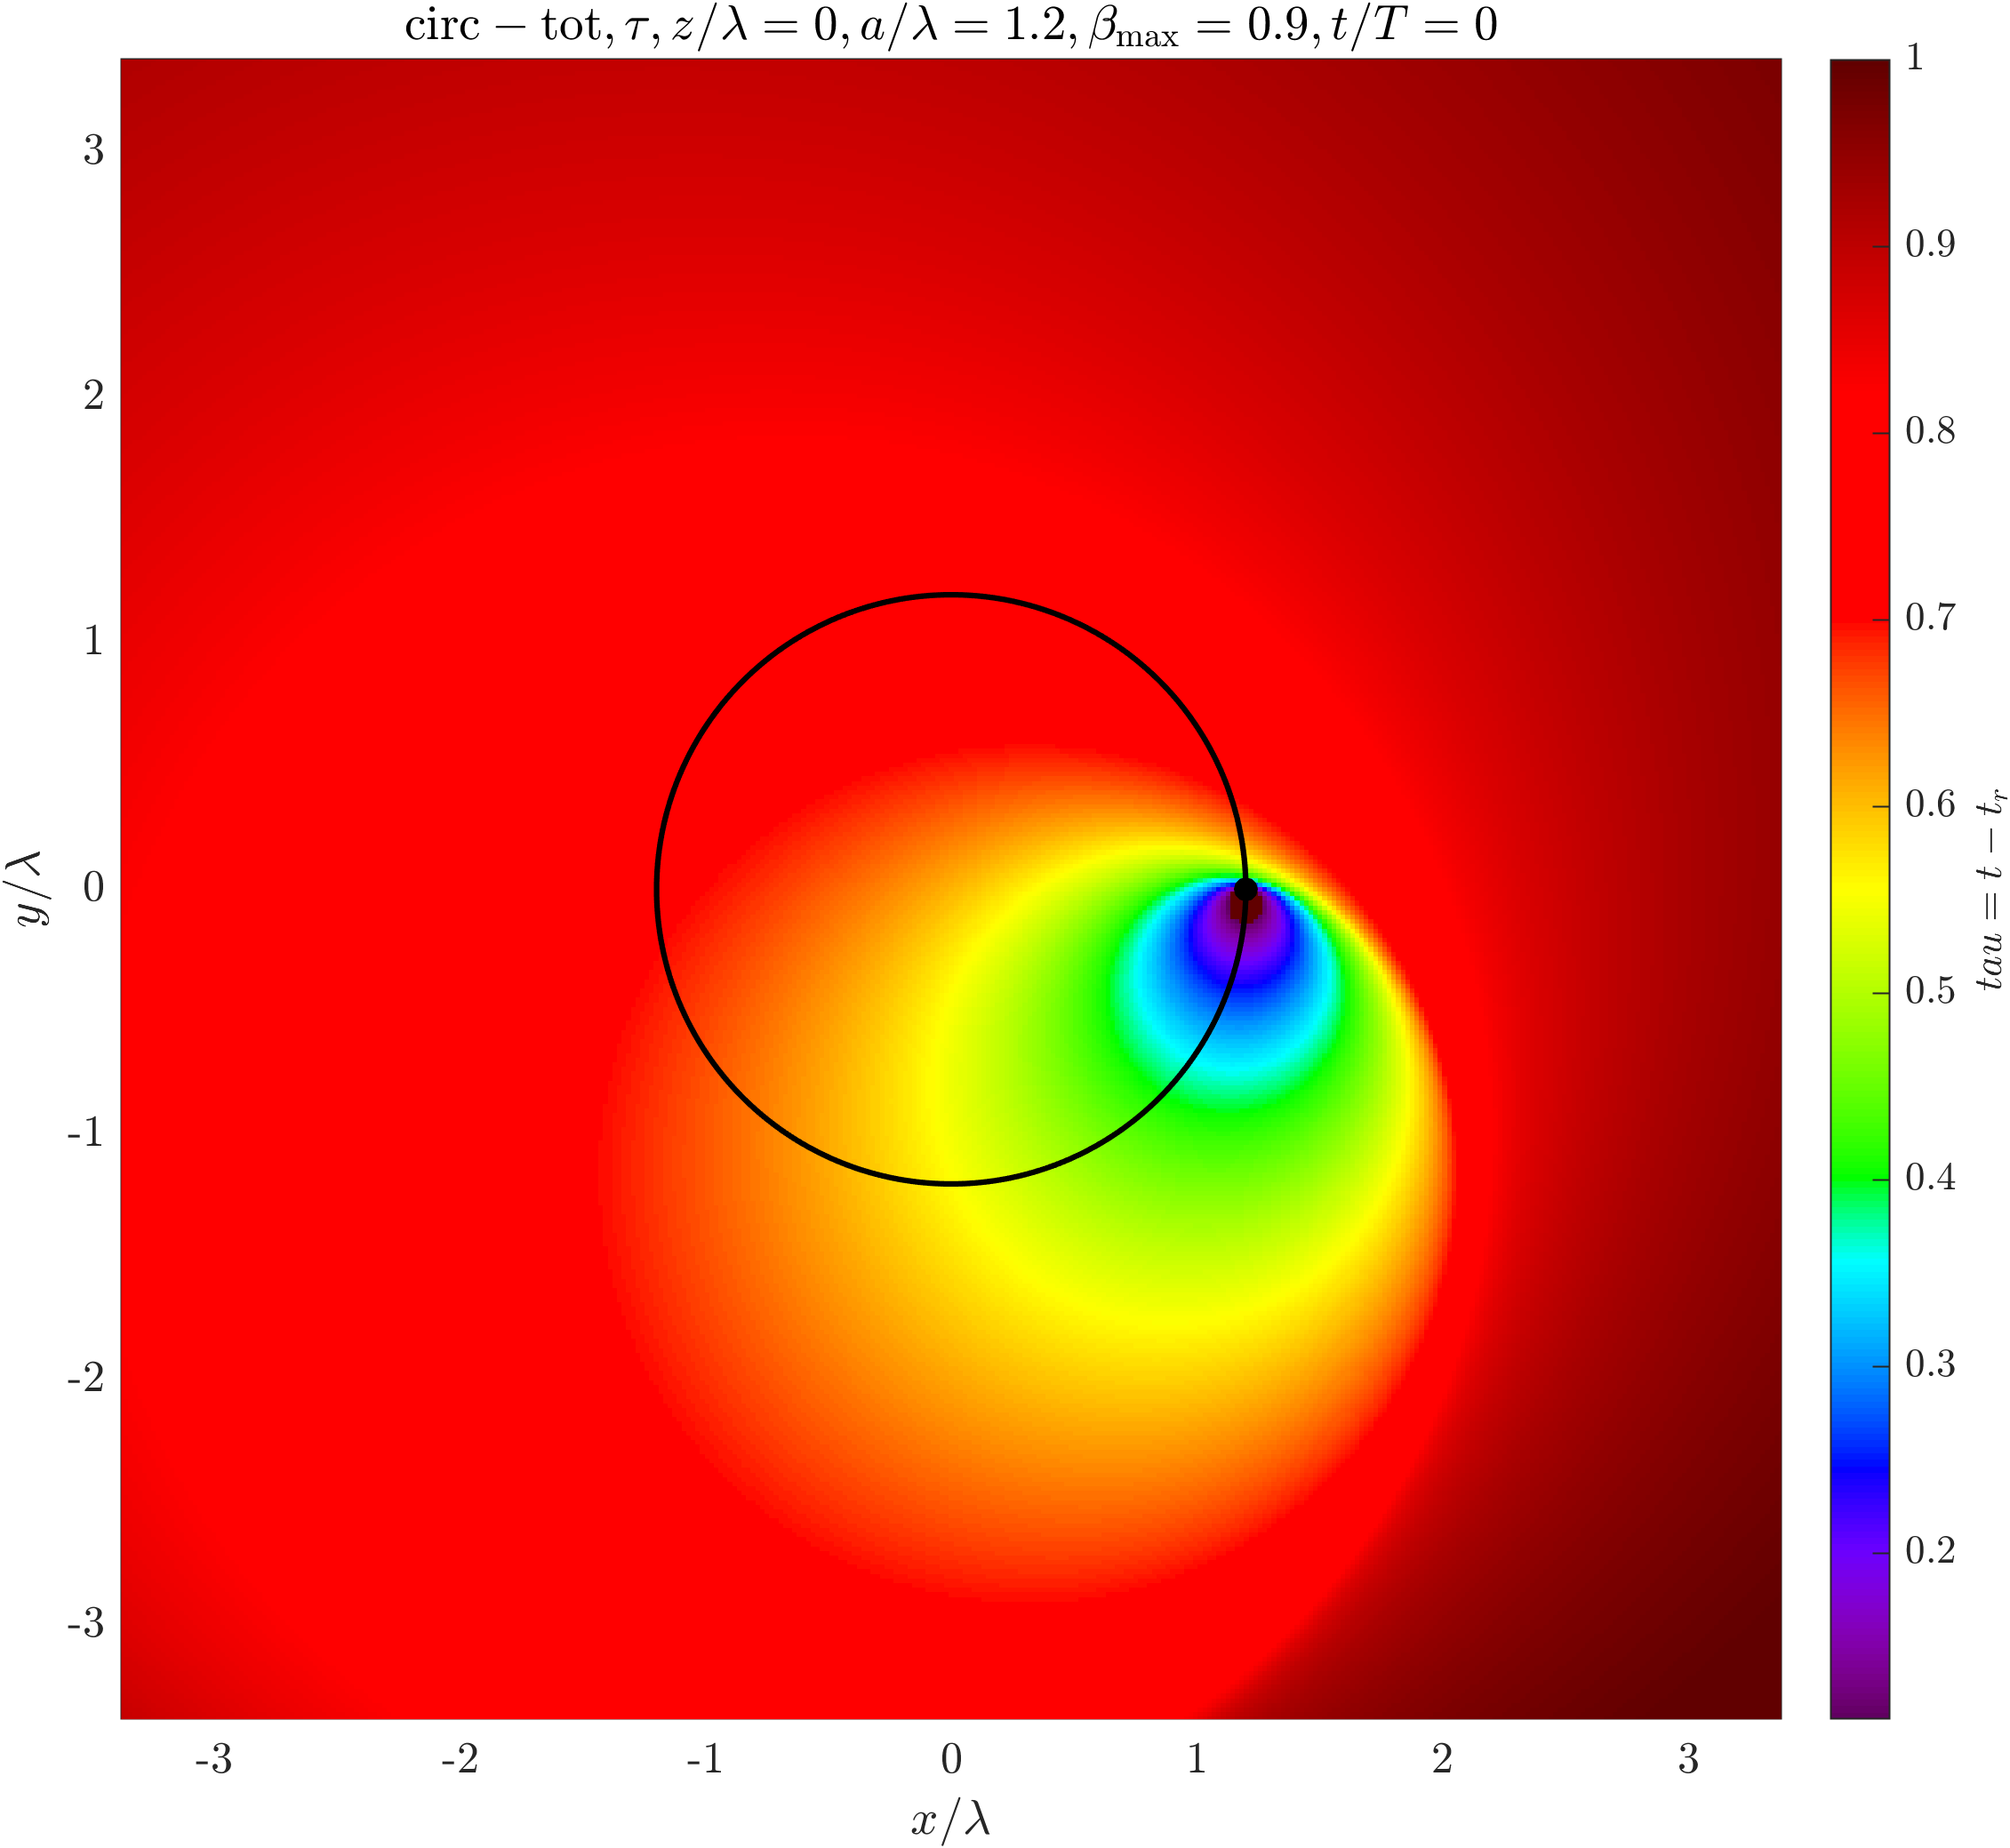
\includegraphics[width=\textwidth]{radiation_fig/circular_motion_tau_xy_beta_0_9.png}
		\caption{\(\tau|_{xy}\) (\(\beta=0.9\))}
		\label{点电荷圆周运动辐射场示意图-tau|_xy(beta=0.9)}
	\end{subfigure}
	\hfill
	\begin{subfigure}[b]{0.23\textwidth}
		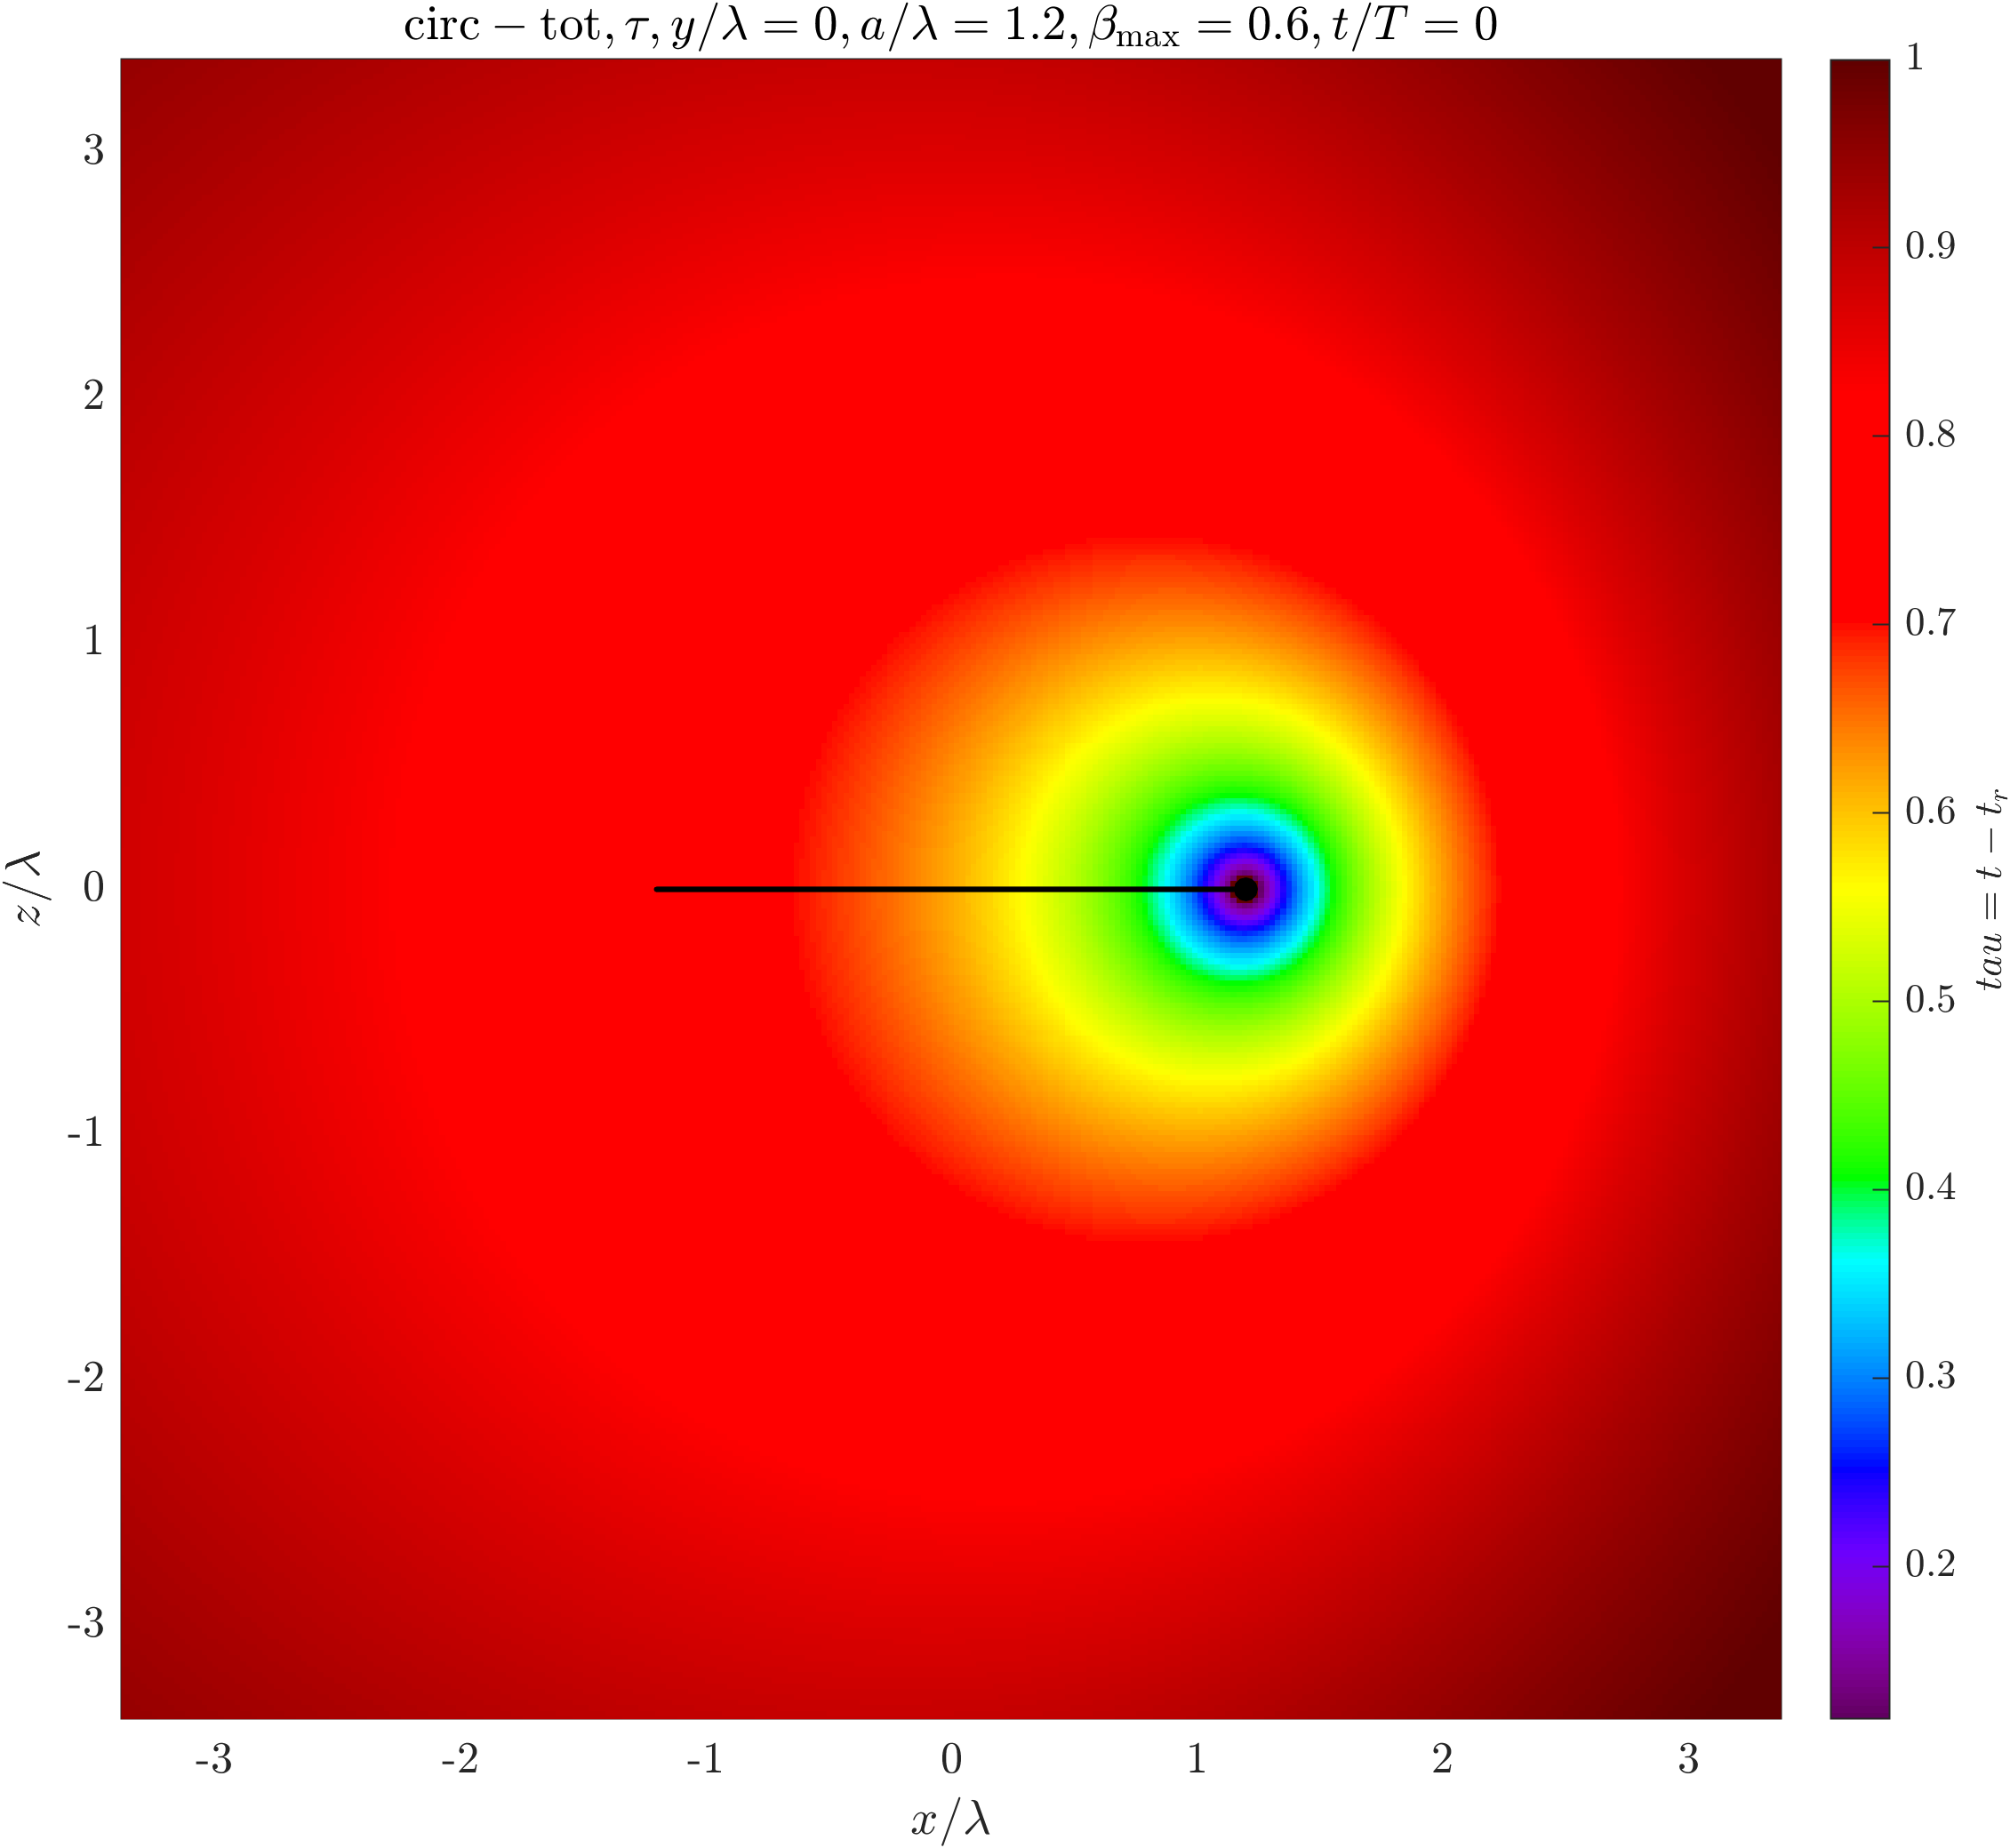
\includegraphics[width=\textwidth]{radiation_fig/circular_motion_tau_xz_beta_0_6.png}
		\caption{\(\tau|_{xz}\) (\(\beta=0.6\))}
		\label{点电荷圆周运动辐射场示意图-tau|_xz(beta=0.6)}
	\end{subfigure}
	\hfill
	\begin{subfigure}[b]{0.23\textwidth}
		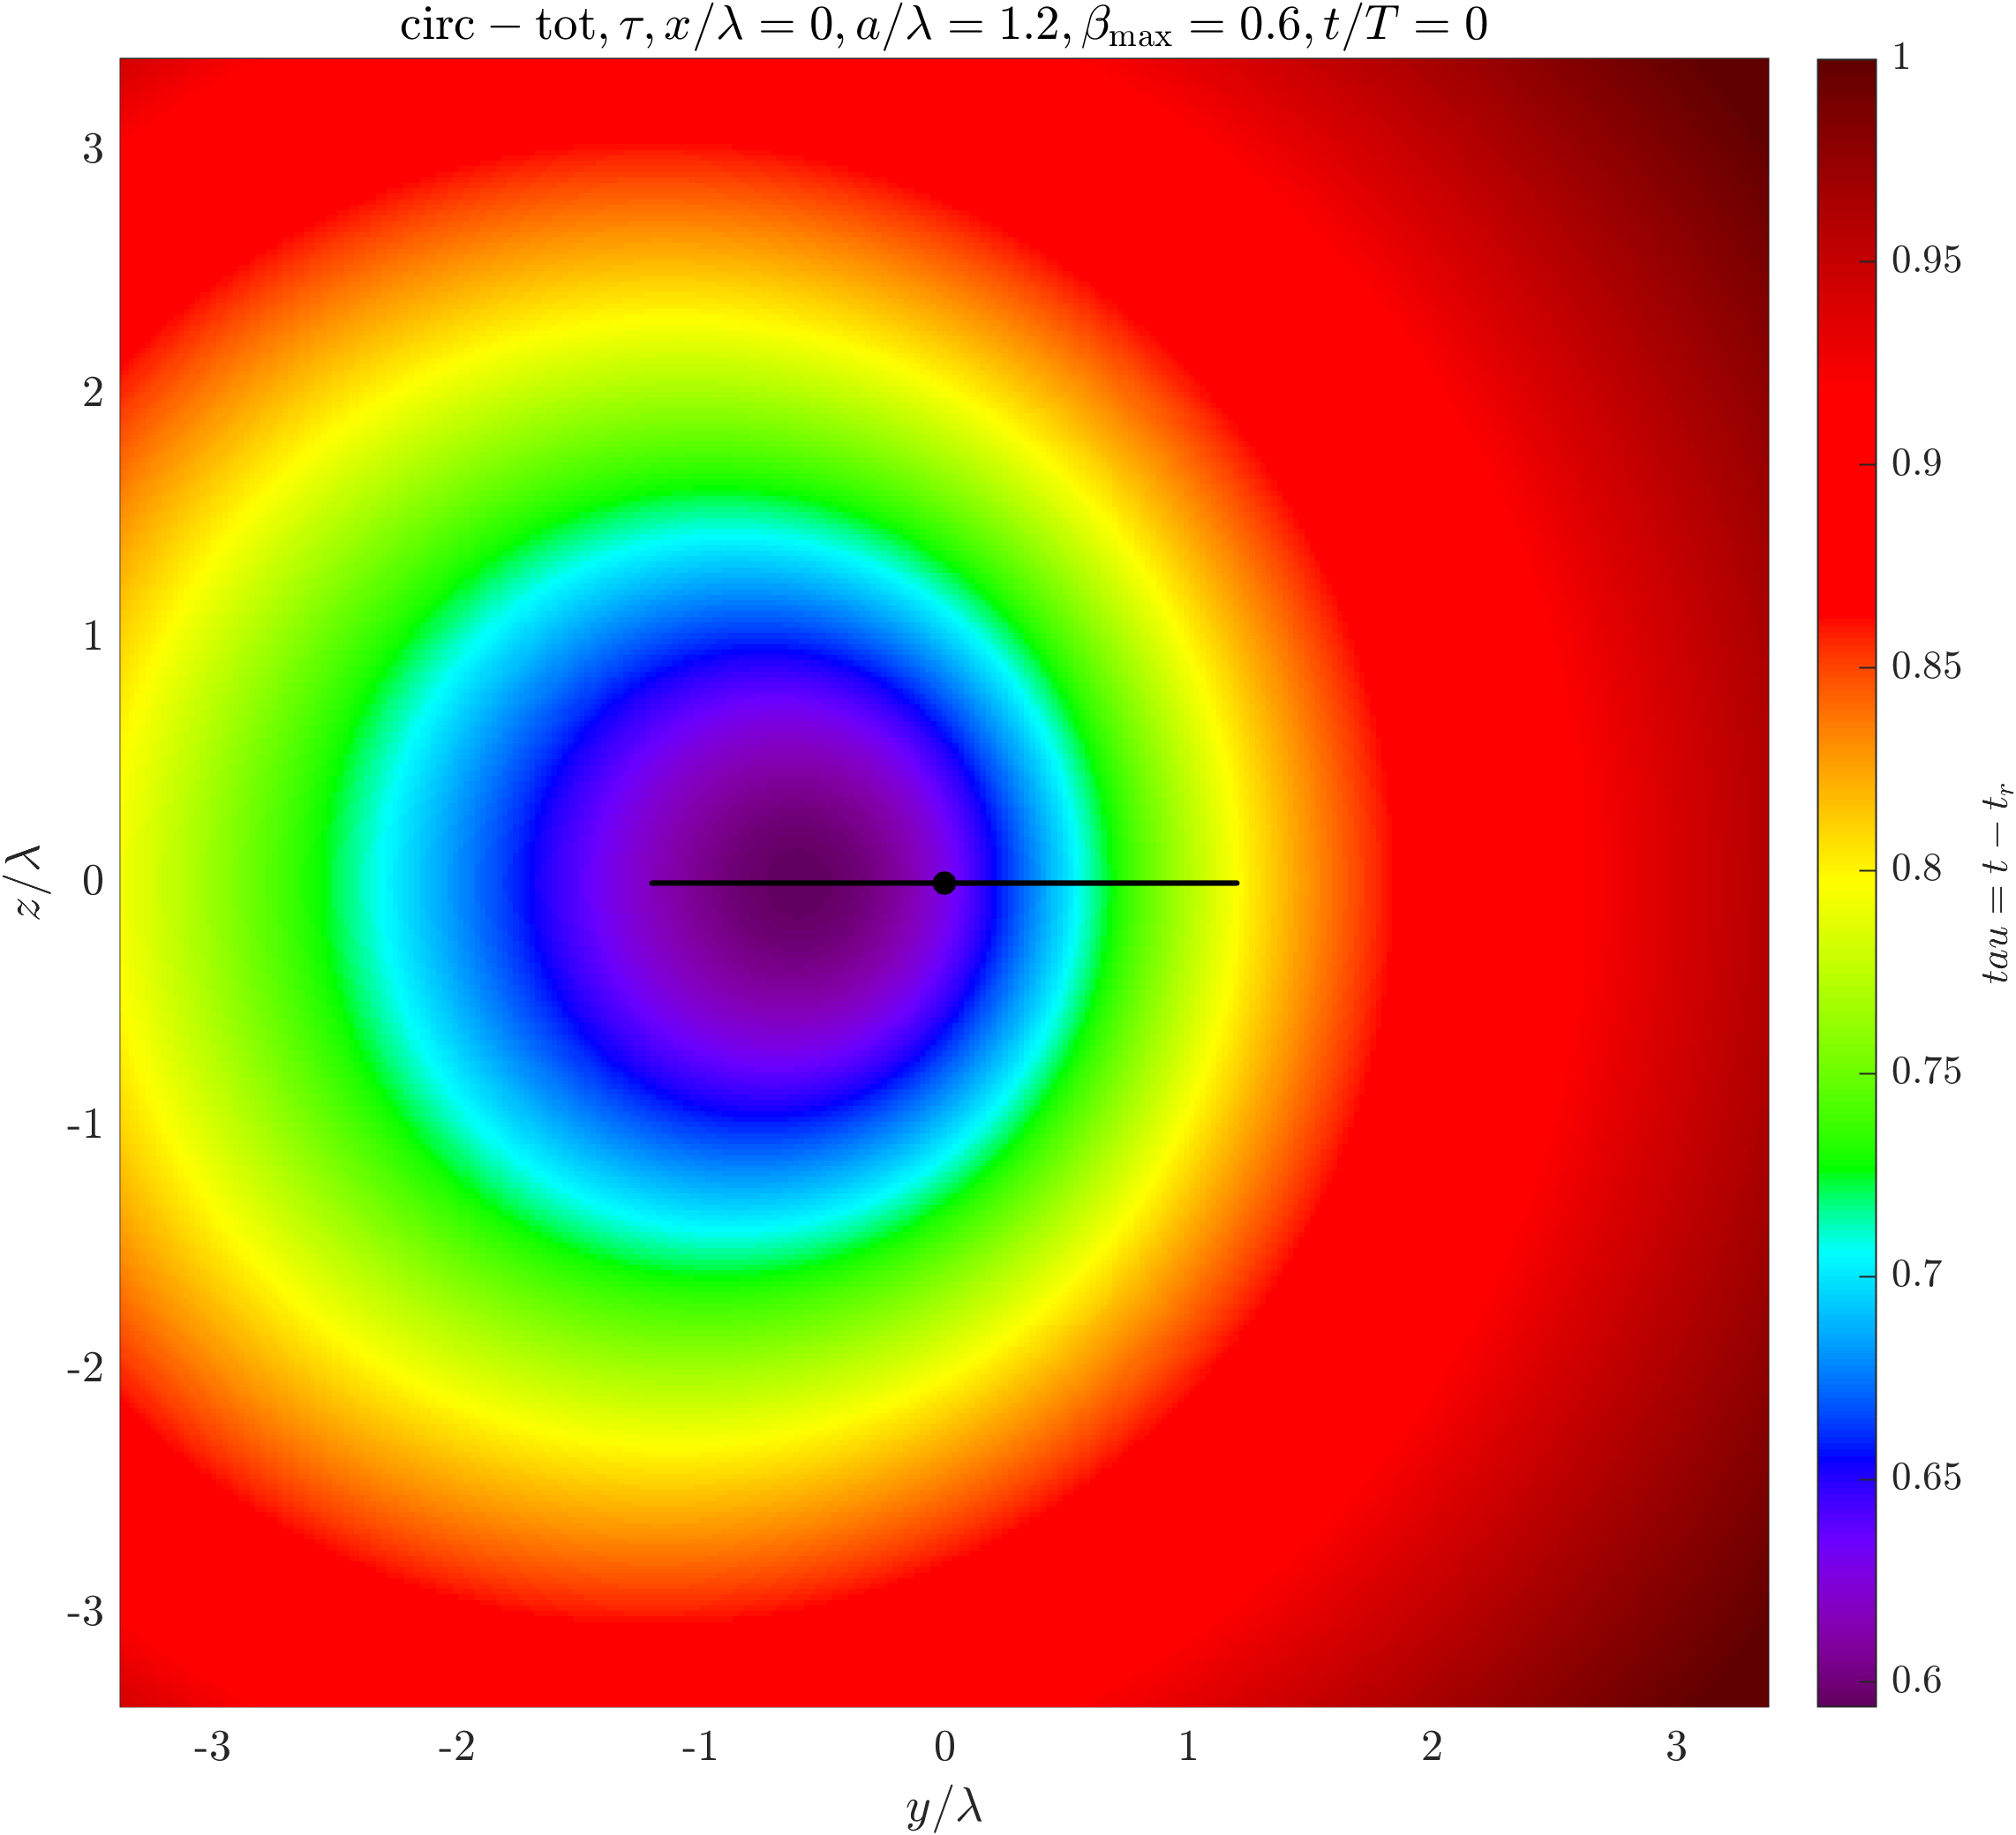
\includegraphics[width=\textwidth]{radiation_fig/circular_motion_tau_yz_beta_0_6.png}
		\caption{\(\tau|_{yz}\) (\(\beta=0.6\))}
		\label{点电荷圆周运动辐射场示意图-tau|_yz(beta=0.6)}
	\end{subfigure}

	\caption{点电荷圆周运动辐射场示意图}
	\label{点电荷圆周运动辐射场示意图}
\end{figure}
\begin{figure}[htbp]
	\centering
	\begin{subfigure}[b]{0.23\textwidth}
		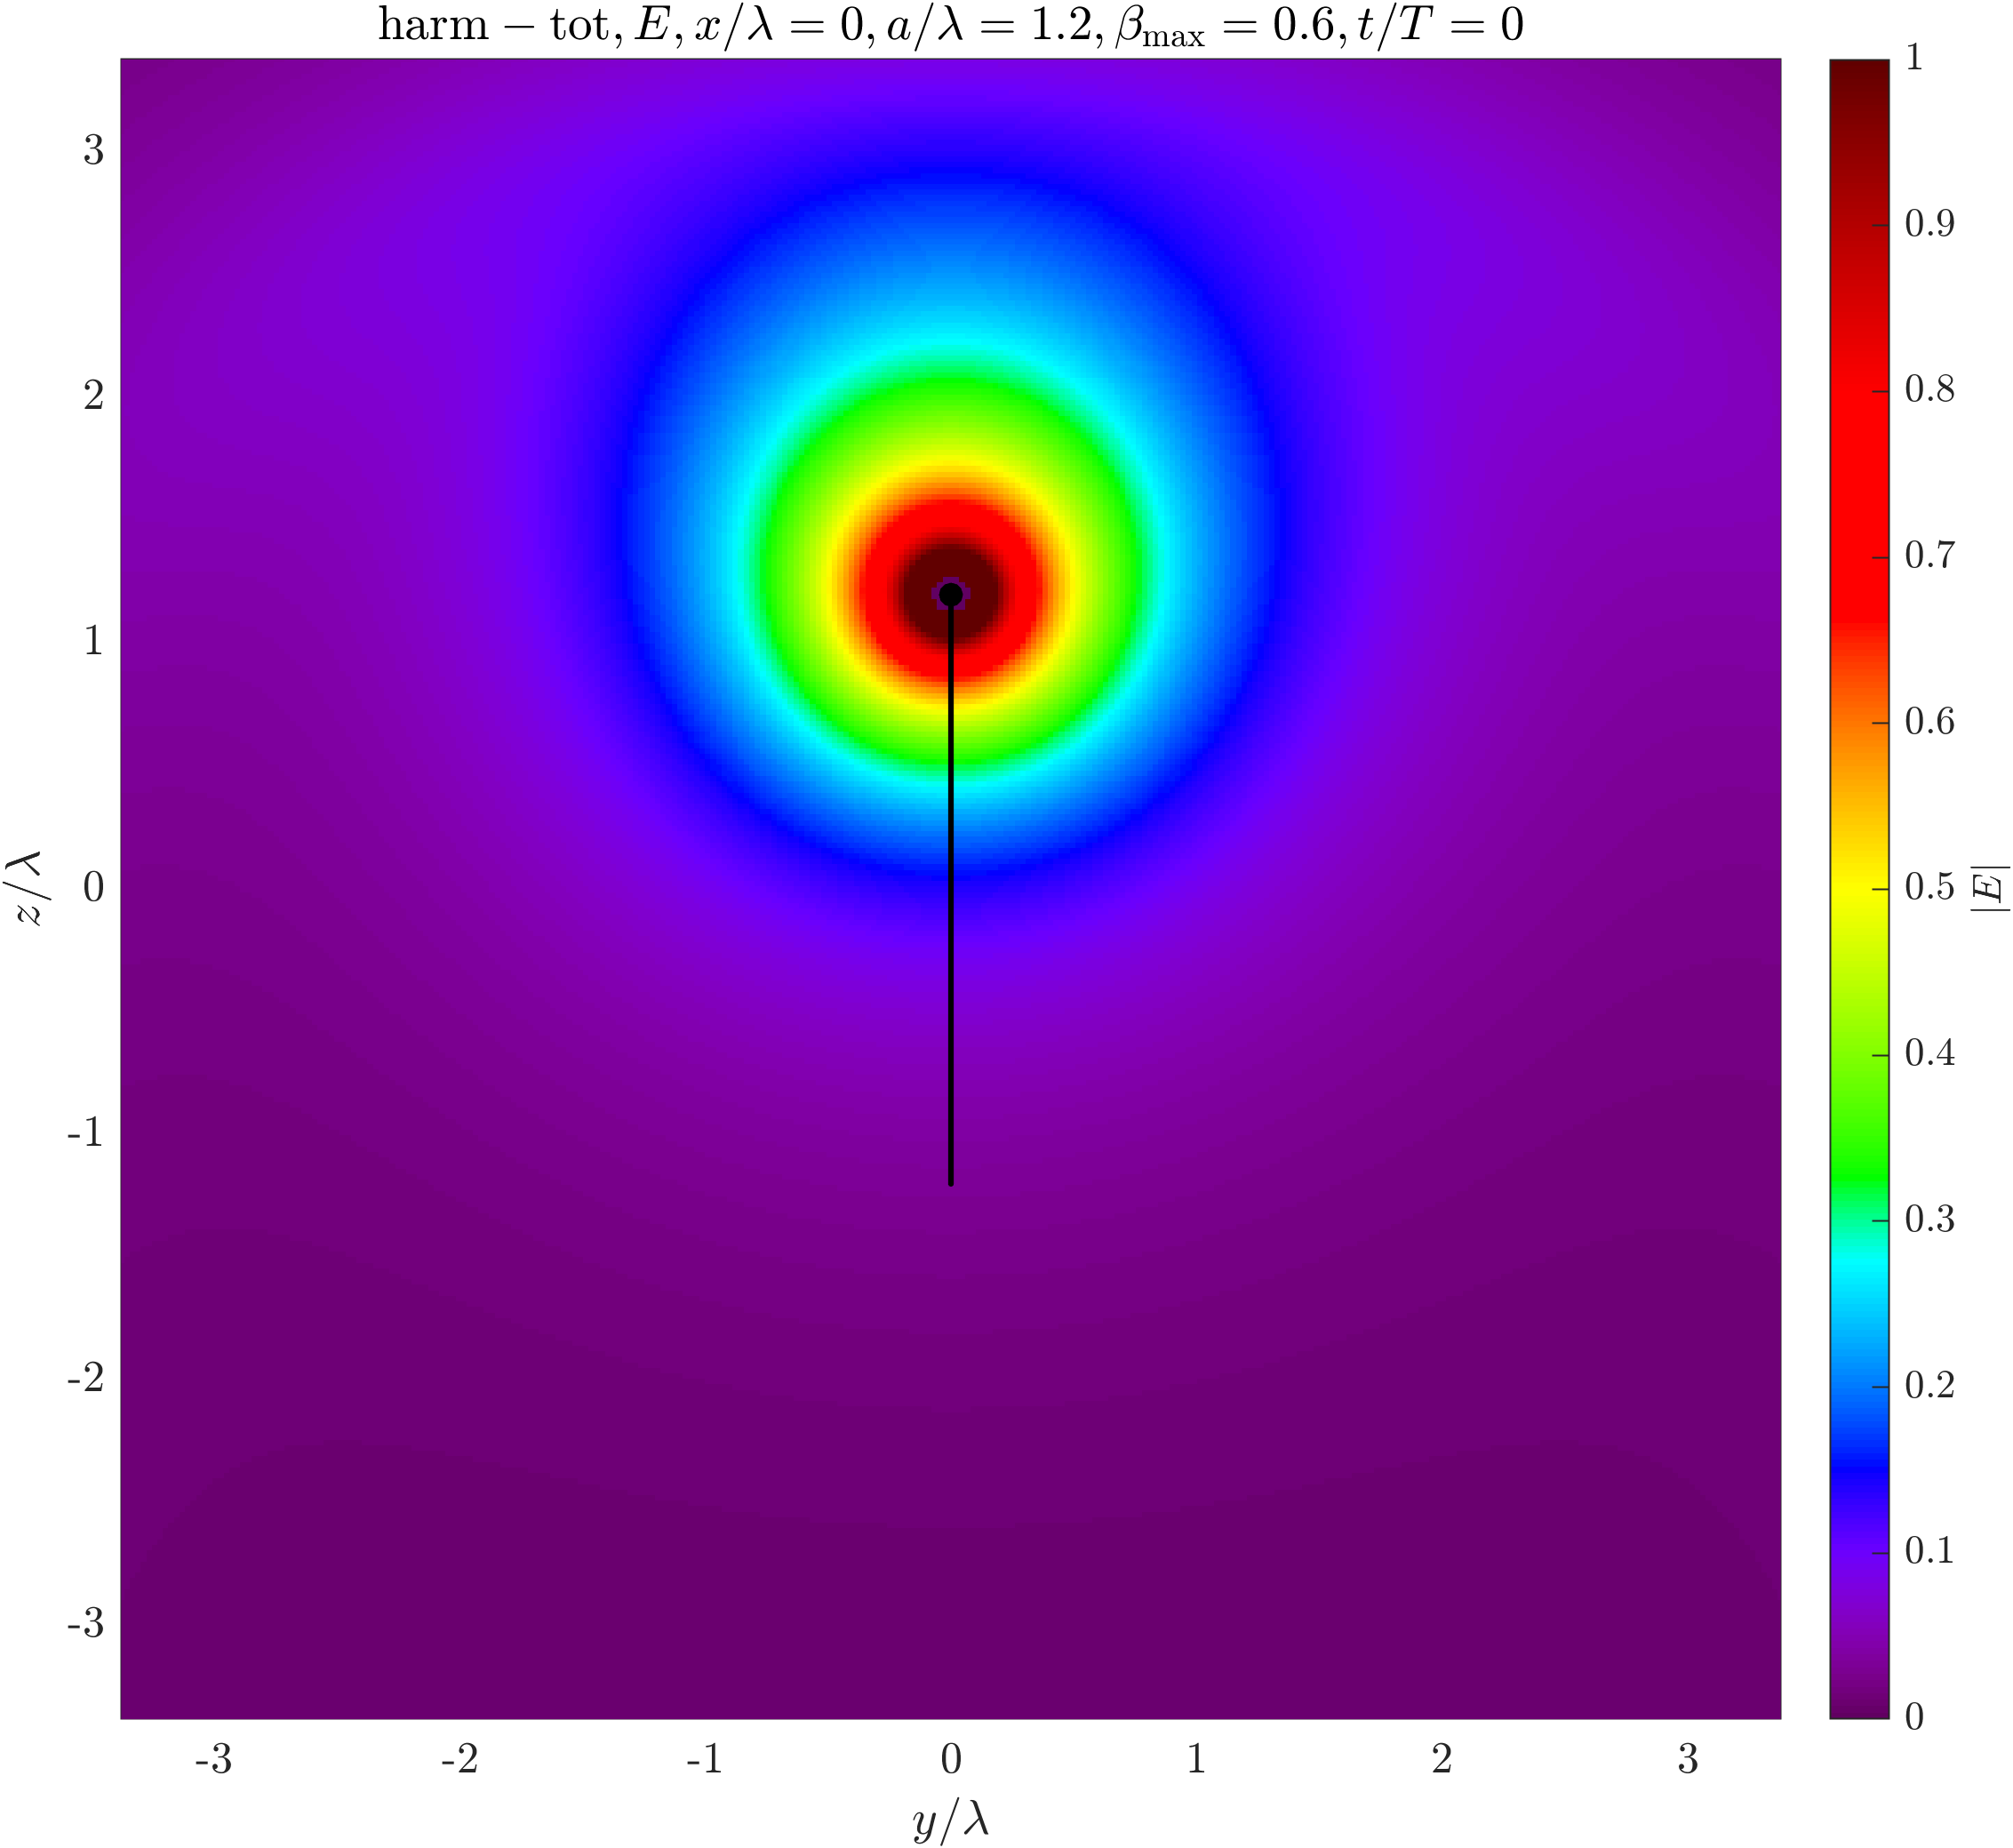
\includegraphics[width=\textwidth]{radiation_fig/harmonic_motion_e_yz_beta_0_6_eta_0.png}
		\caption{\(E|_{yz}\) (\(\beta=0.6\), \(\eta=0\))}
		\label{点电荷简谐运动辐射场示意图-E|_yz(beta=0.6,eta=0)}
	\end{subfigure}
	\hfill
	\begin{subfigure}[b]{0.23\textwidth}
		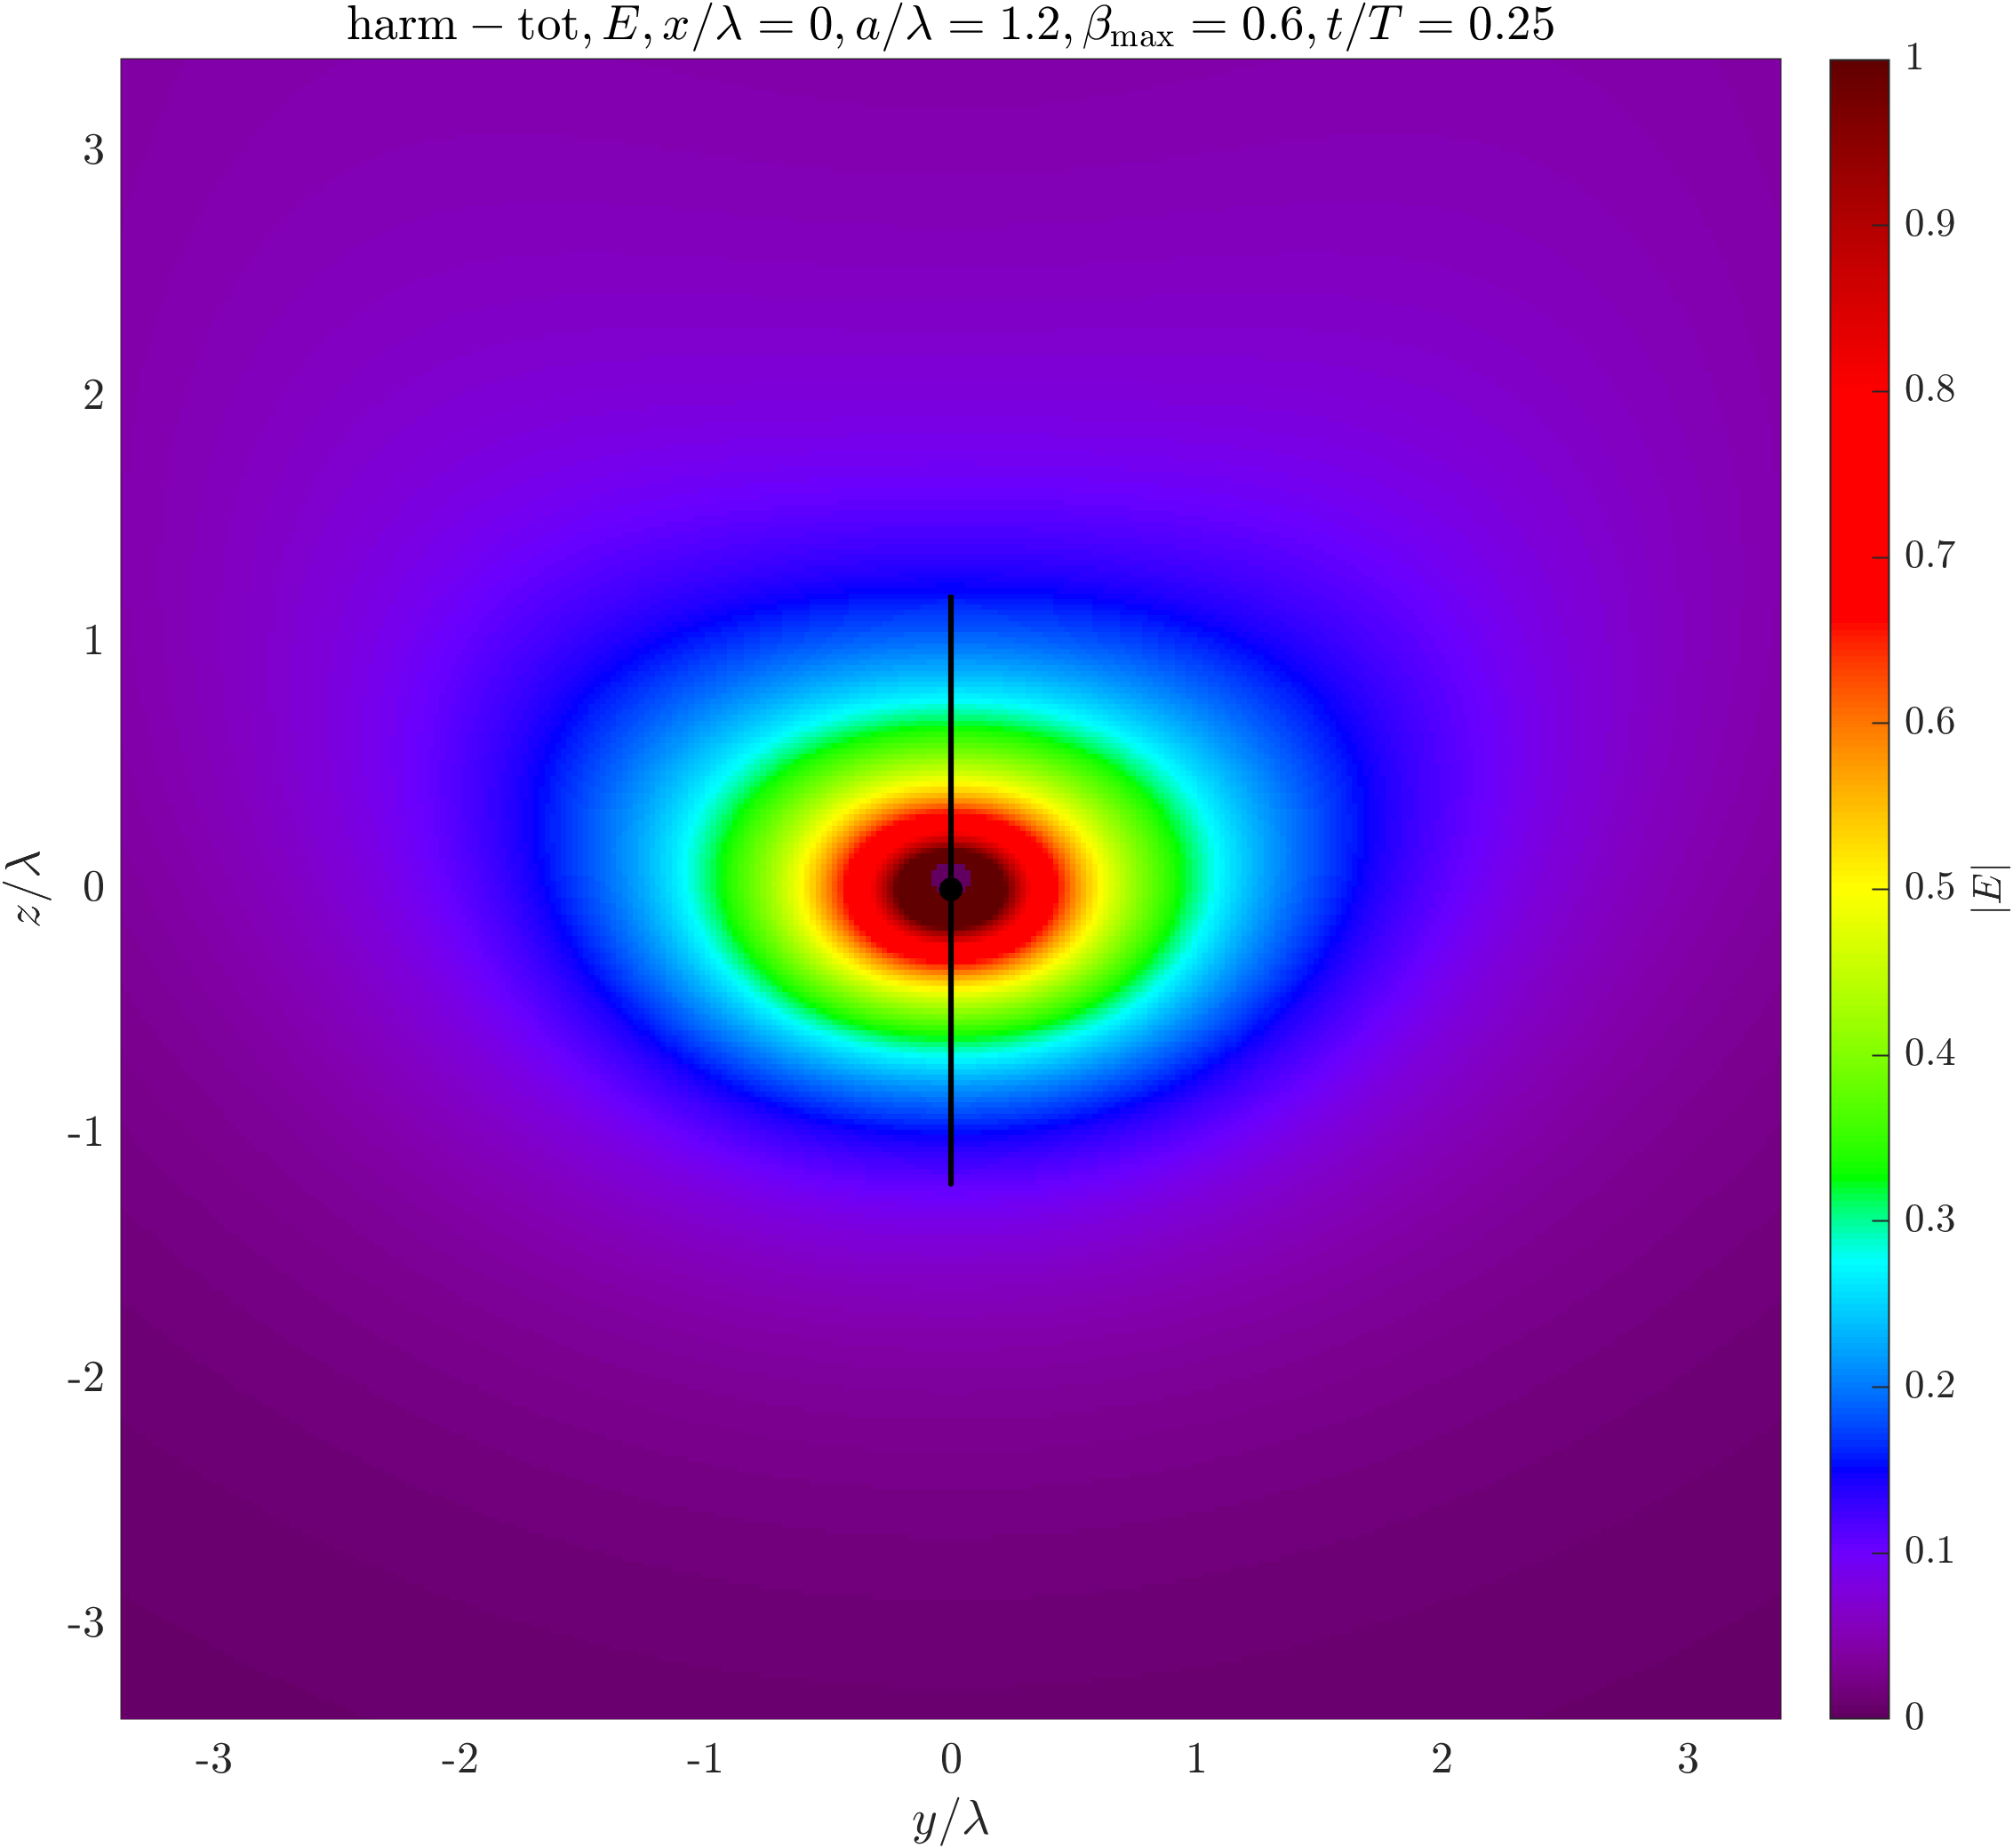
\includegraphics[width=\textwidth]{radiation_fig/harmonic_motion_e_yz_beta_0_6_eta_0_25.png}
		\caption{\(E|_{yz}\) (\(\beta=0.6\), \(\eta=0.25\))}
		\label{点电荷简谐运动辐射场示意图-E|_yz(beta=0.6,eta=0.25)}
	\end{subfigure}
	\hfill
	\begin{subfigure}[b]{0.23\textwidth}
		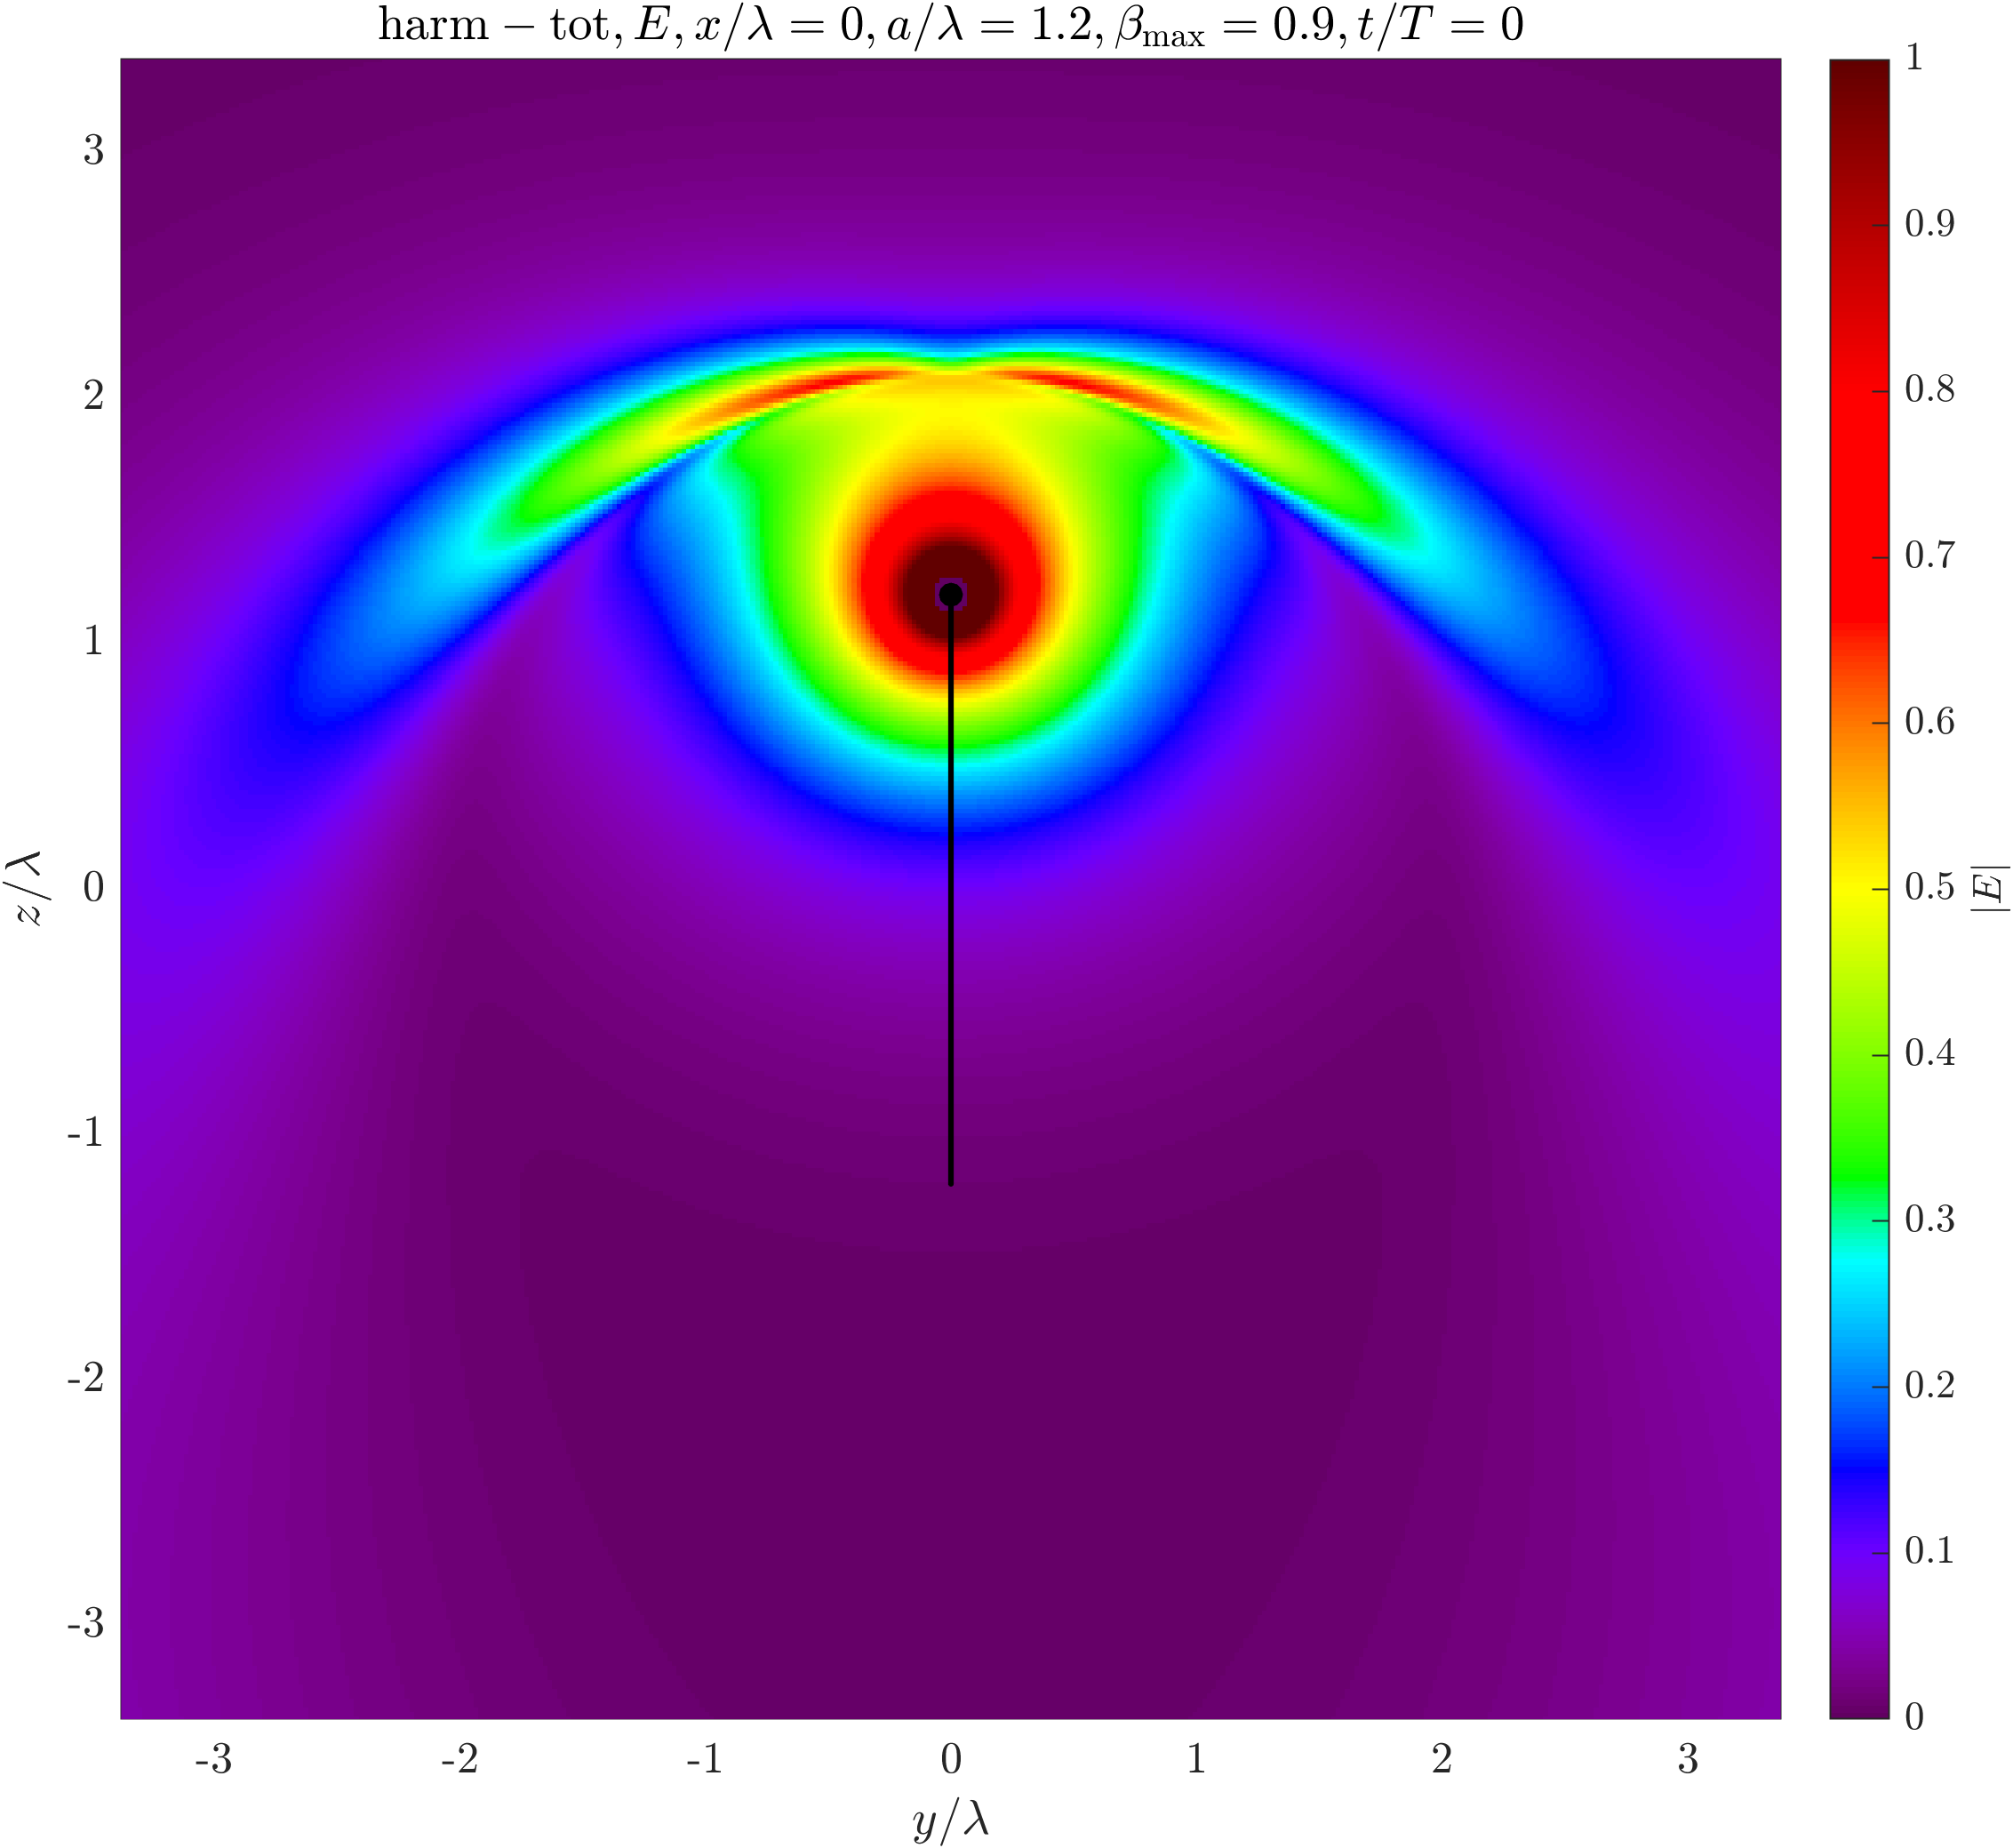
\includegraphics[width=\textwidth]{radiation_fig/harmonic_motion_e_yz_beta_0_9_eta_0.png}
		\caption{\(E|_{yz}\) (\(\beta=0.9\), \(\eta=0\))}
		\label{点电荷简谐运动辐射场示意图-E|_yz(beta=0.9,eta=0)}
	\end{subfigure}
	\hfill
	\begin{subfigure}[b]{0.23\textwidth}
		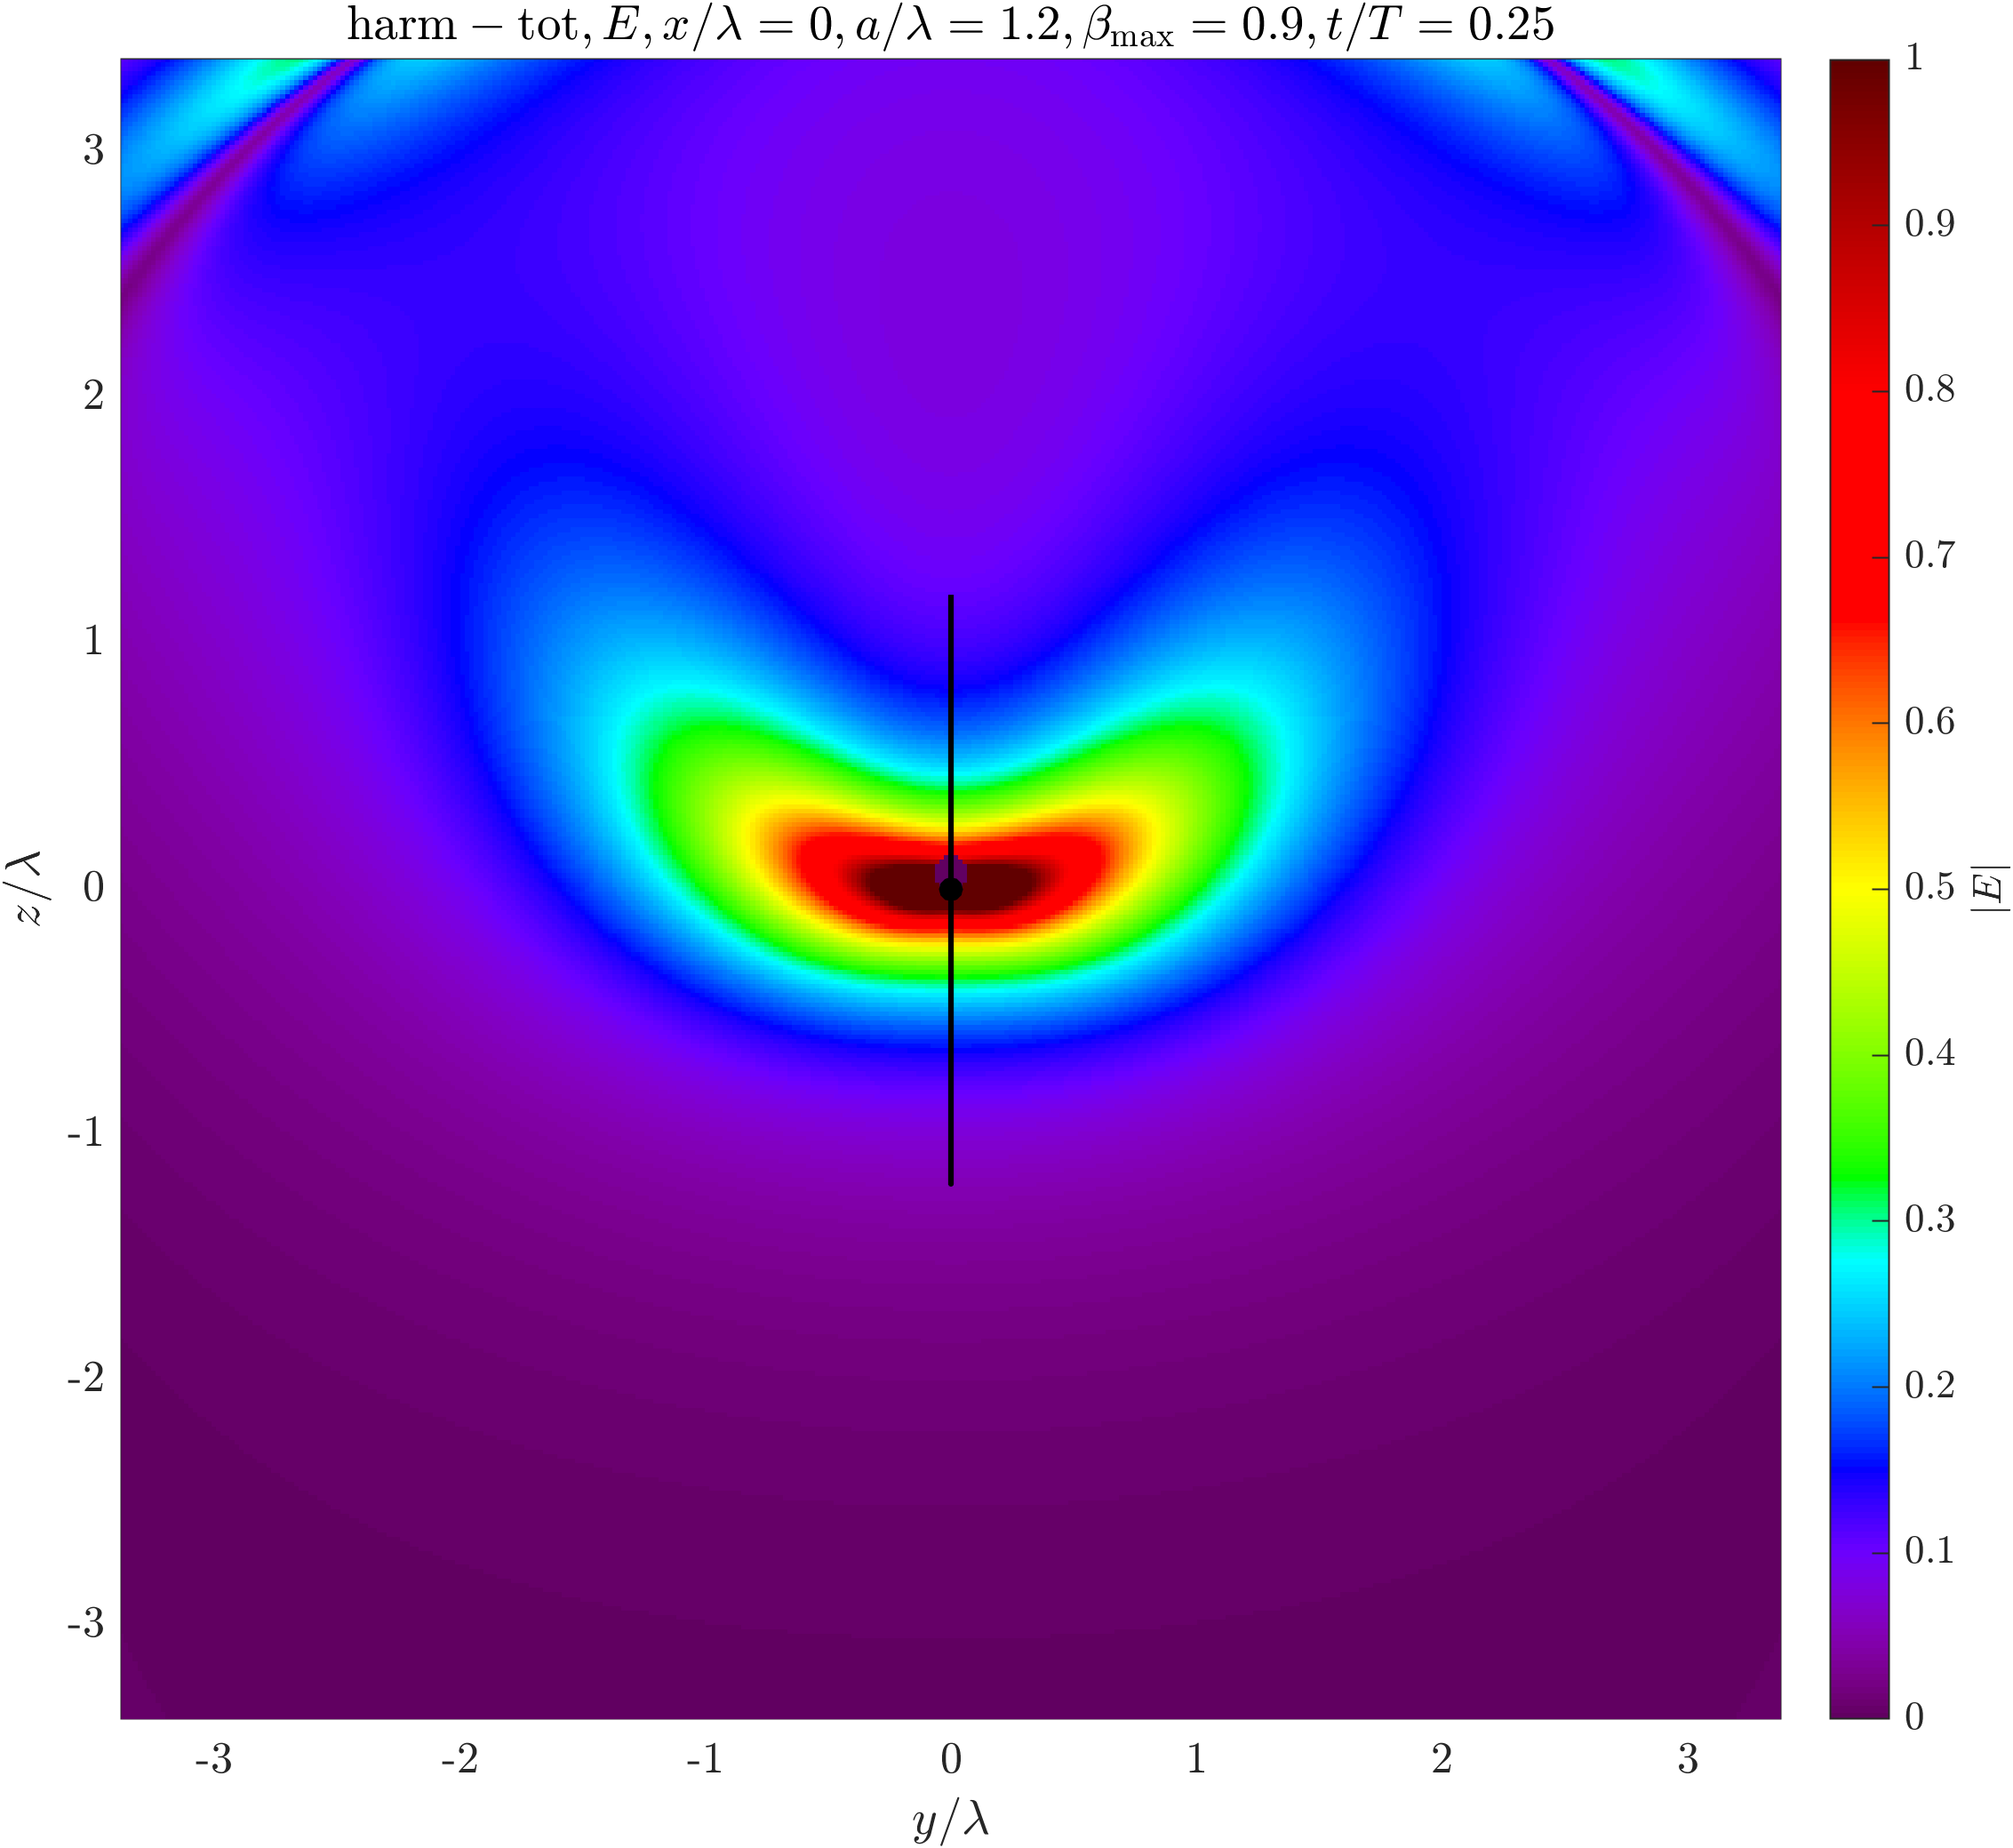
\includegraphics[width=\textwidth]{radiation_fig/harmonic_motion_e_yz_beta_0_9_eta_0_25.png}
		\caption{\(E|_{yz}\) (\(\beta=0.9\), \(\eta=0.25\))}
		\label{点电荷简谐运动辐射场示意图-E|_yz(beta=0.9,eta=0.25)}
	\end{subfigure}
	\vspace{0.2cm}
	\begin{subfigure}[b]{0.23\textwidth}
		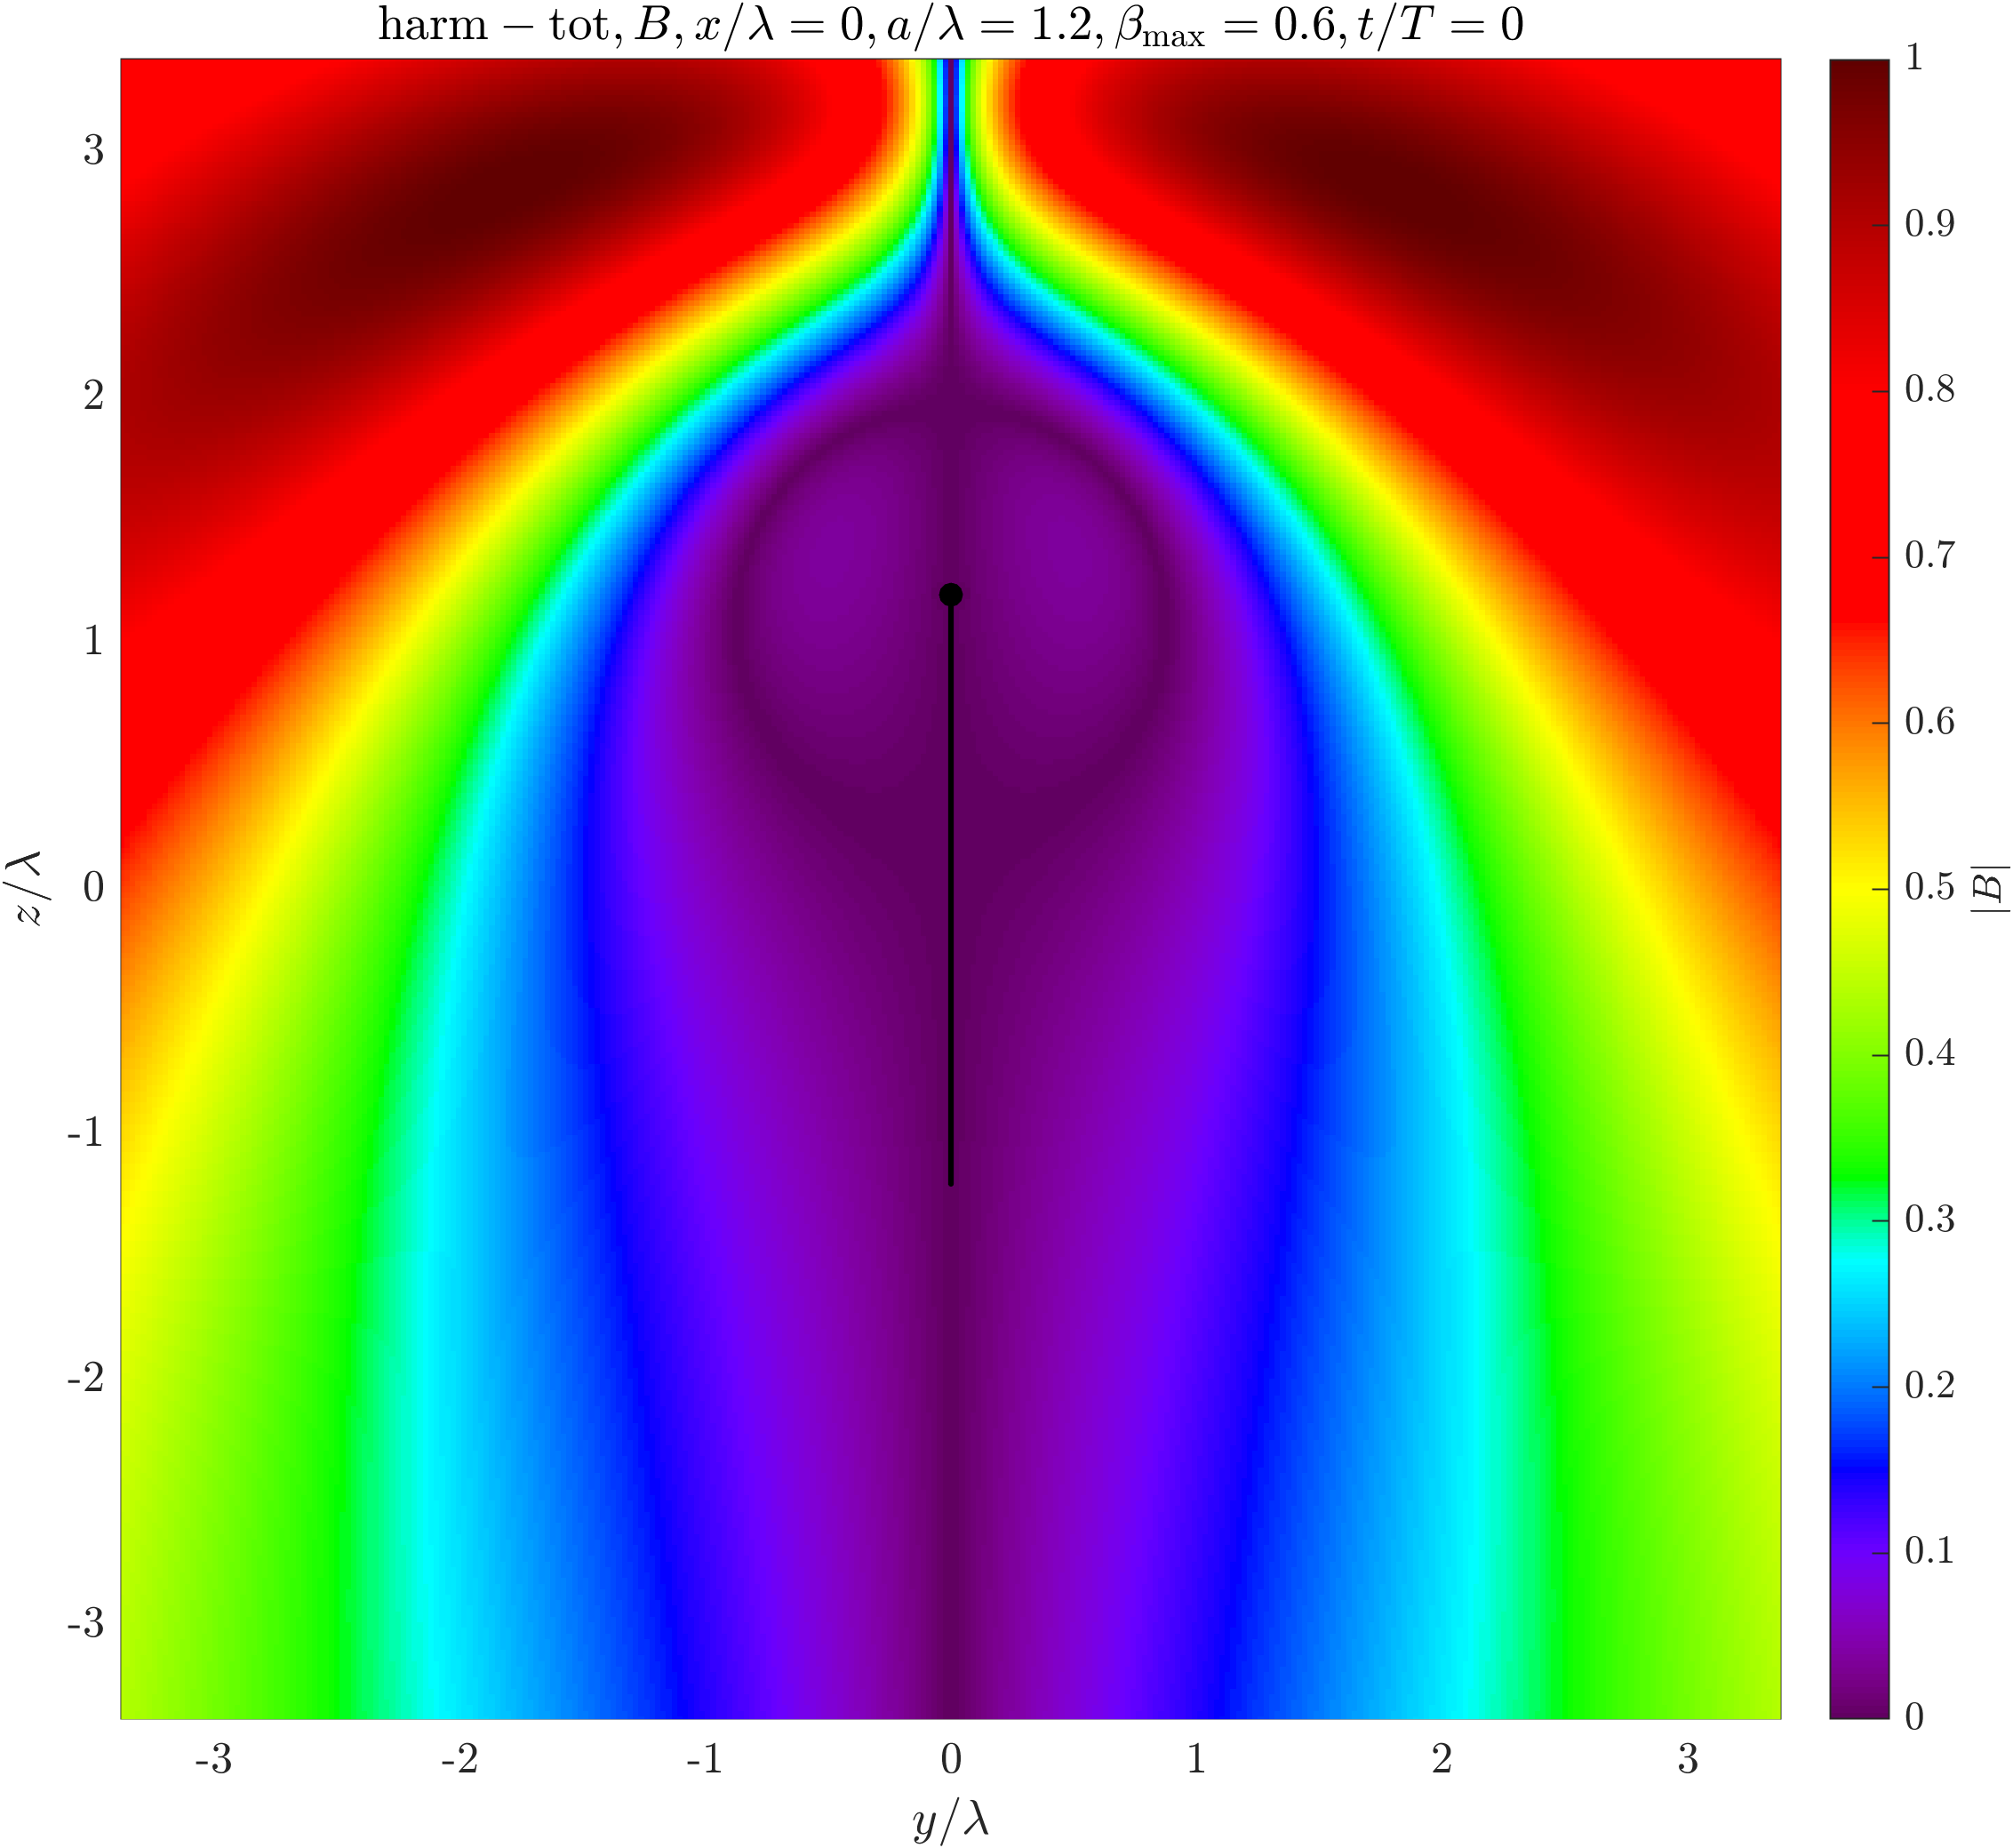
\includegraphics[width=\textwidth]{radiation_fig/harmonic_motion_b_yz_beta_0_6_eta_0.png}
		\caption{\(B|_{yz}\) (\(\beta=0.6\), \(\eta=0\))}
		\label{点电荷简谐运动辐射场示意图-B|_yz(beta=0.6,eta=0)}
	\end{subfigure}
	\hfill
	\begin{subfigure}[b]{0.23\textwidth}
		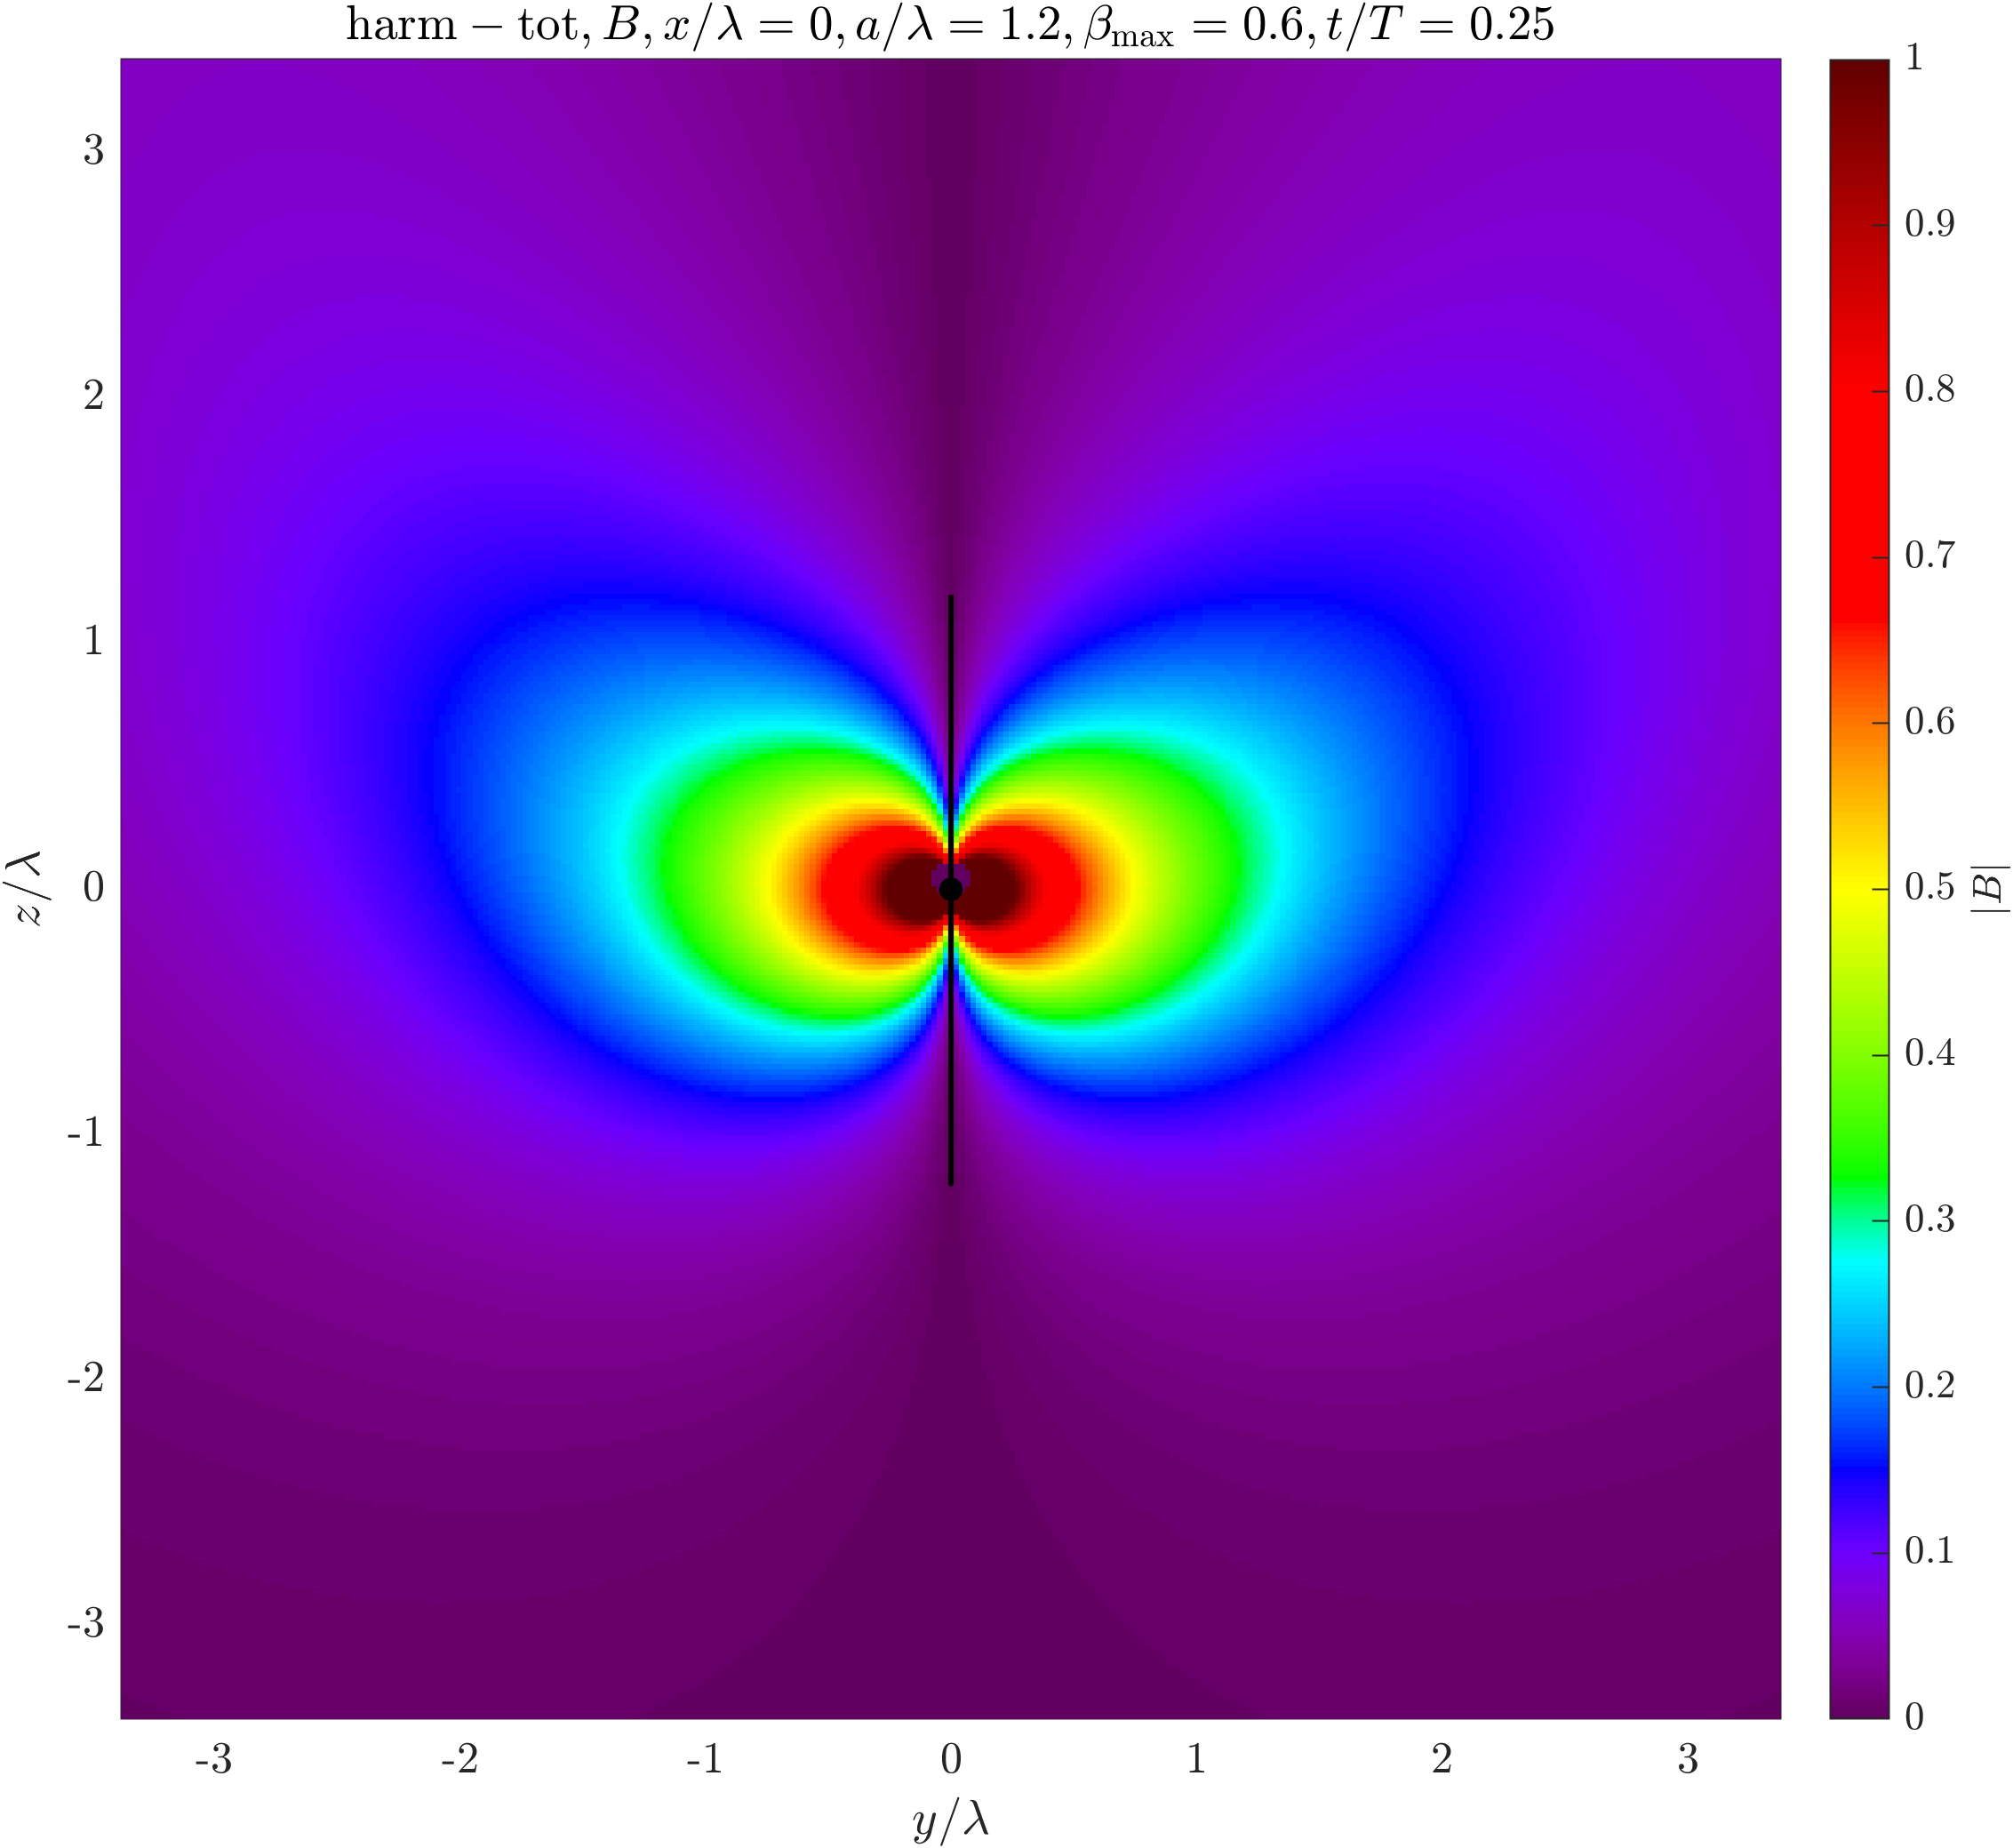
\includegraphics[width=\textwidth]{radiation_fig/harmonic_motion_b_yz_beta_0_6_eta_0_25.png}
		\caption{\(B|_{yz}\) (\(\beta=0.6\), \(\eta=0.25\))}
		\label{点电荷简谐运动辐射场示意图-B|_yz(beta=0.6,eta=0.25)}
	\end{subfigure}
	\hfill
	\begin{subfigure}[b]{0.23\textwidth}
		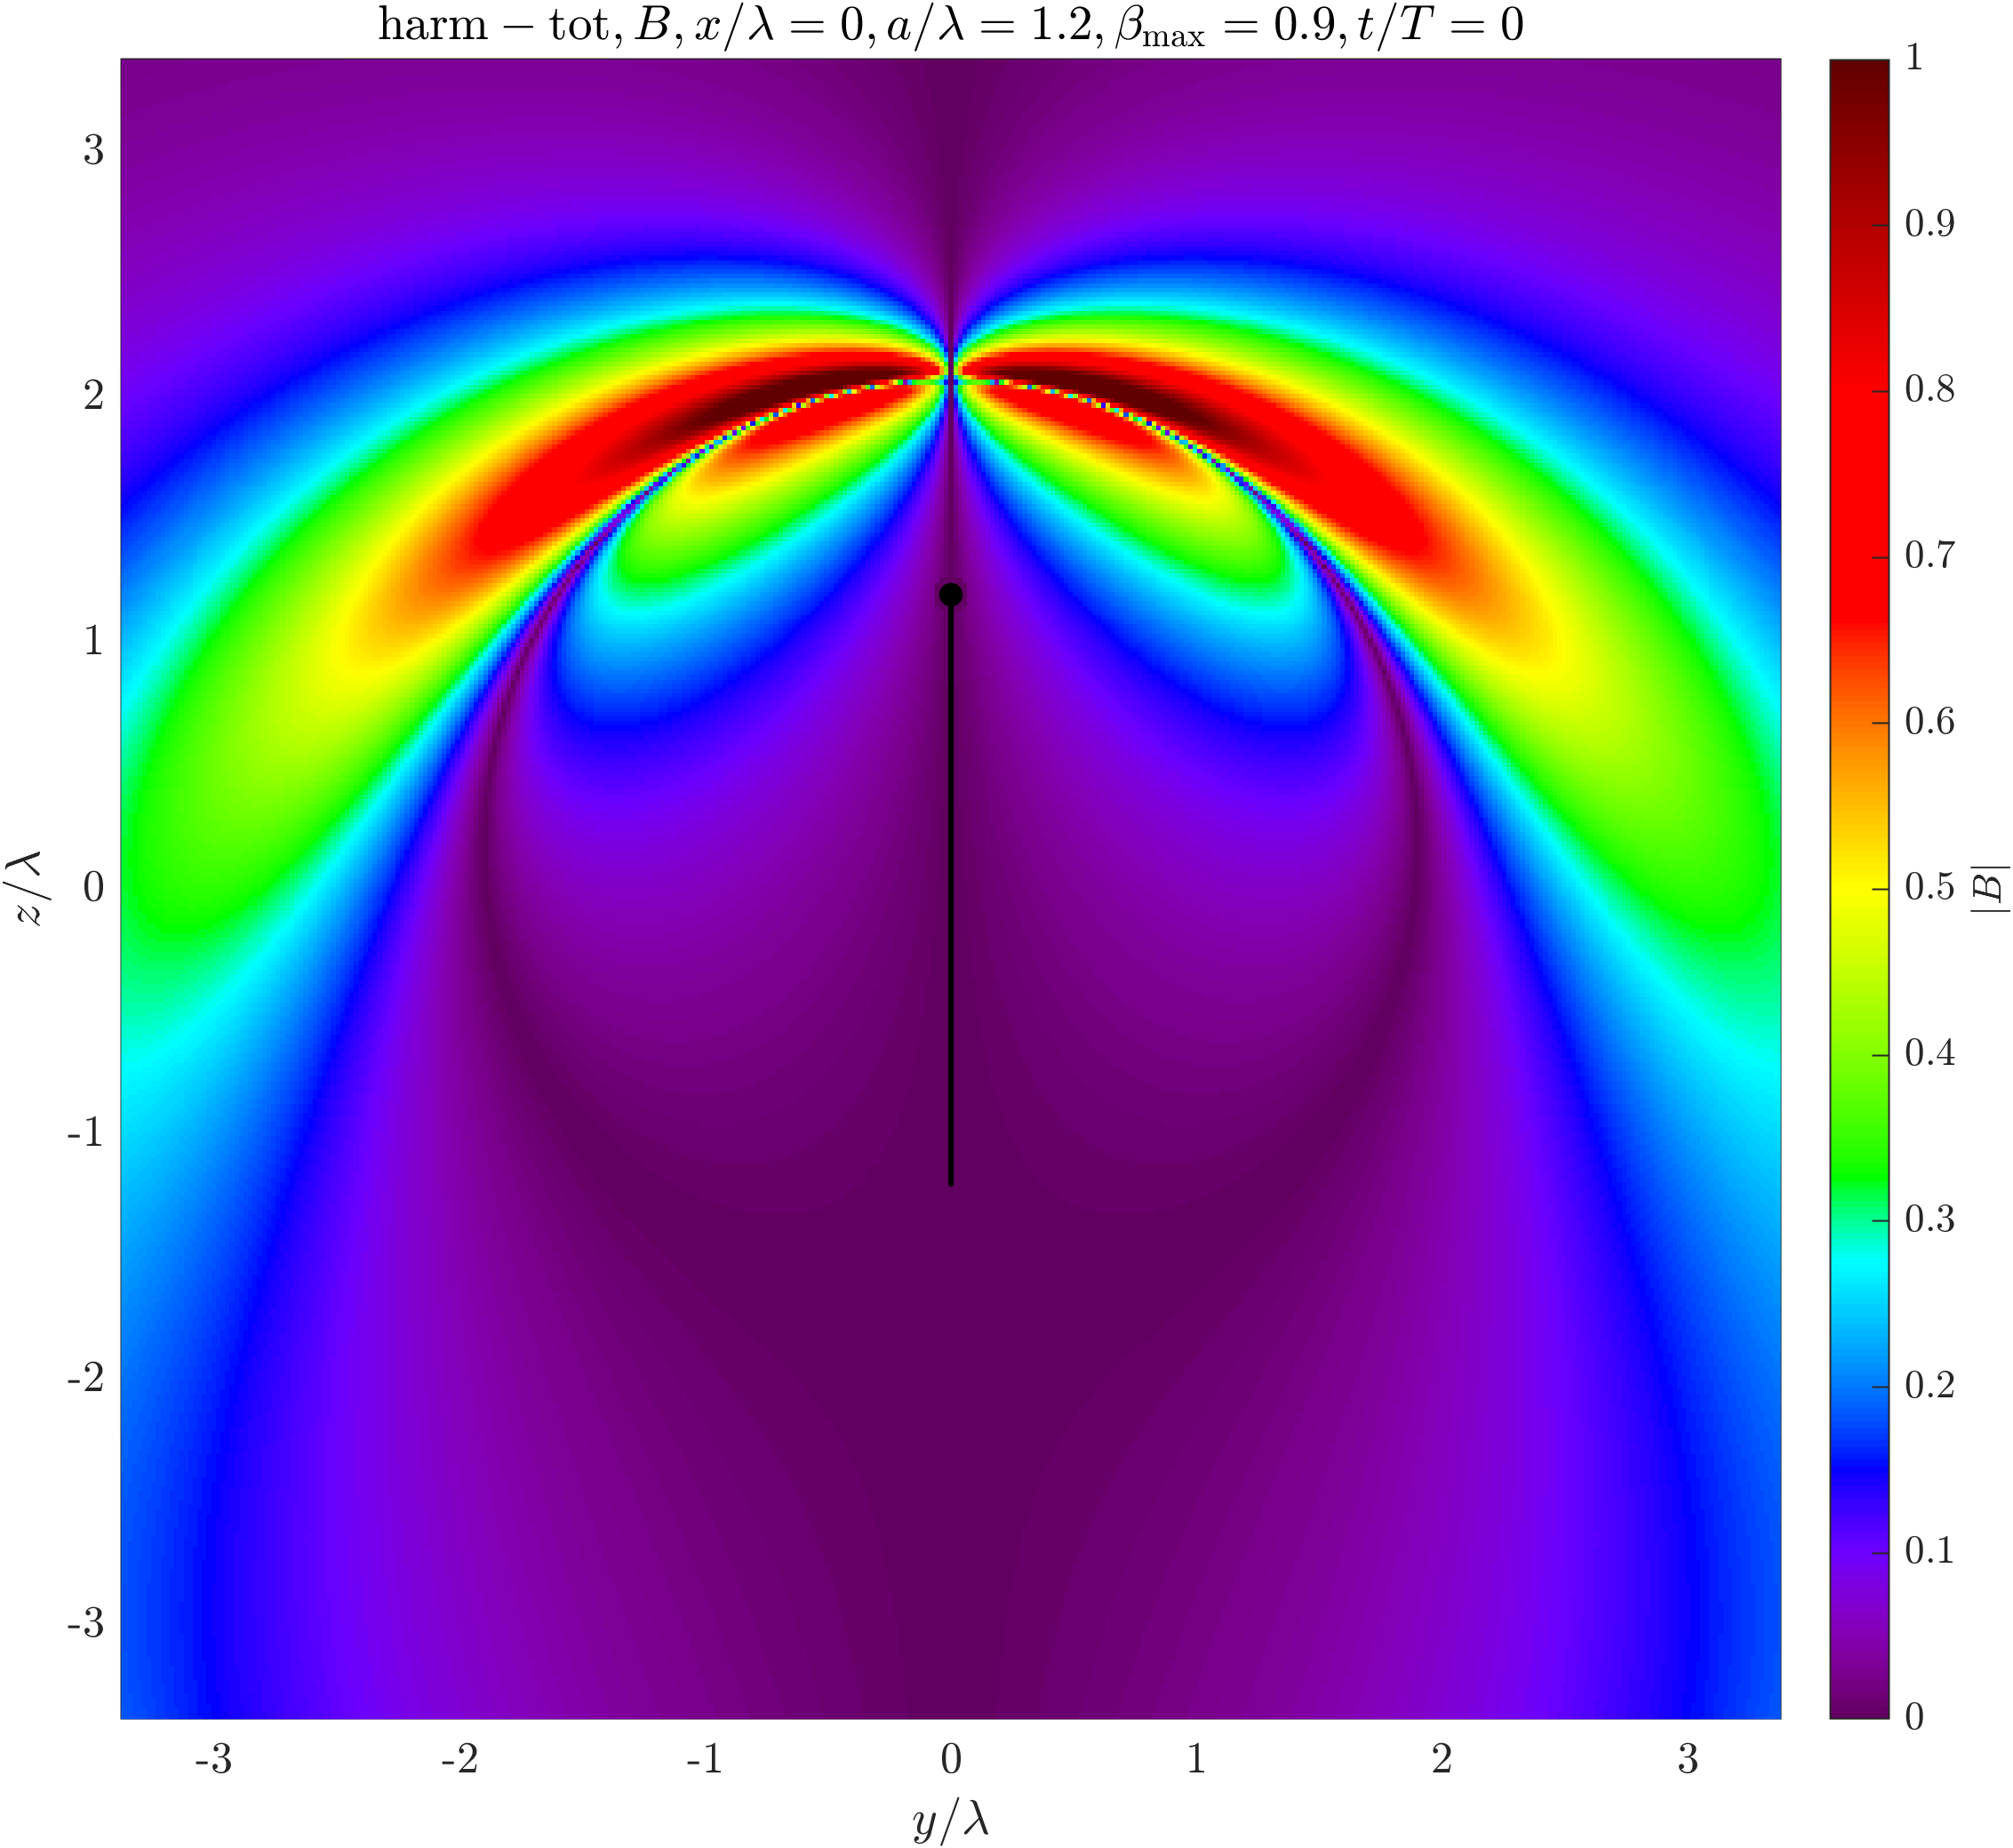
\includegraphics[width=\textwidth]{radiation_fig/harmonic_motion_b_yz_beta_0_9_eta_0.png}
		\caption{\(B|_{yz}\) (\(\beta=0.9\), \(\eta=0\))}
		\label{点电荷简谐运动辐射场示意图-B|_yz(beta=0.9,eta=0)}
	\end{subfigure}
	\hfill
	\begin{subfigure}[b]{0.23\textwidth}
		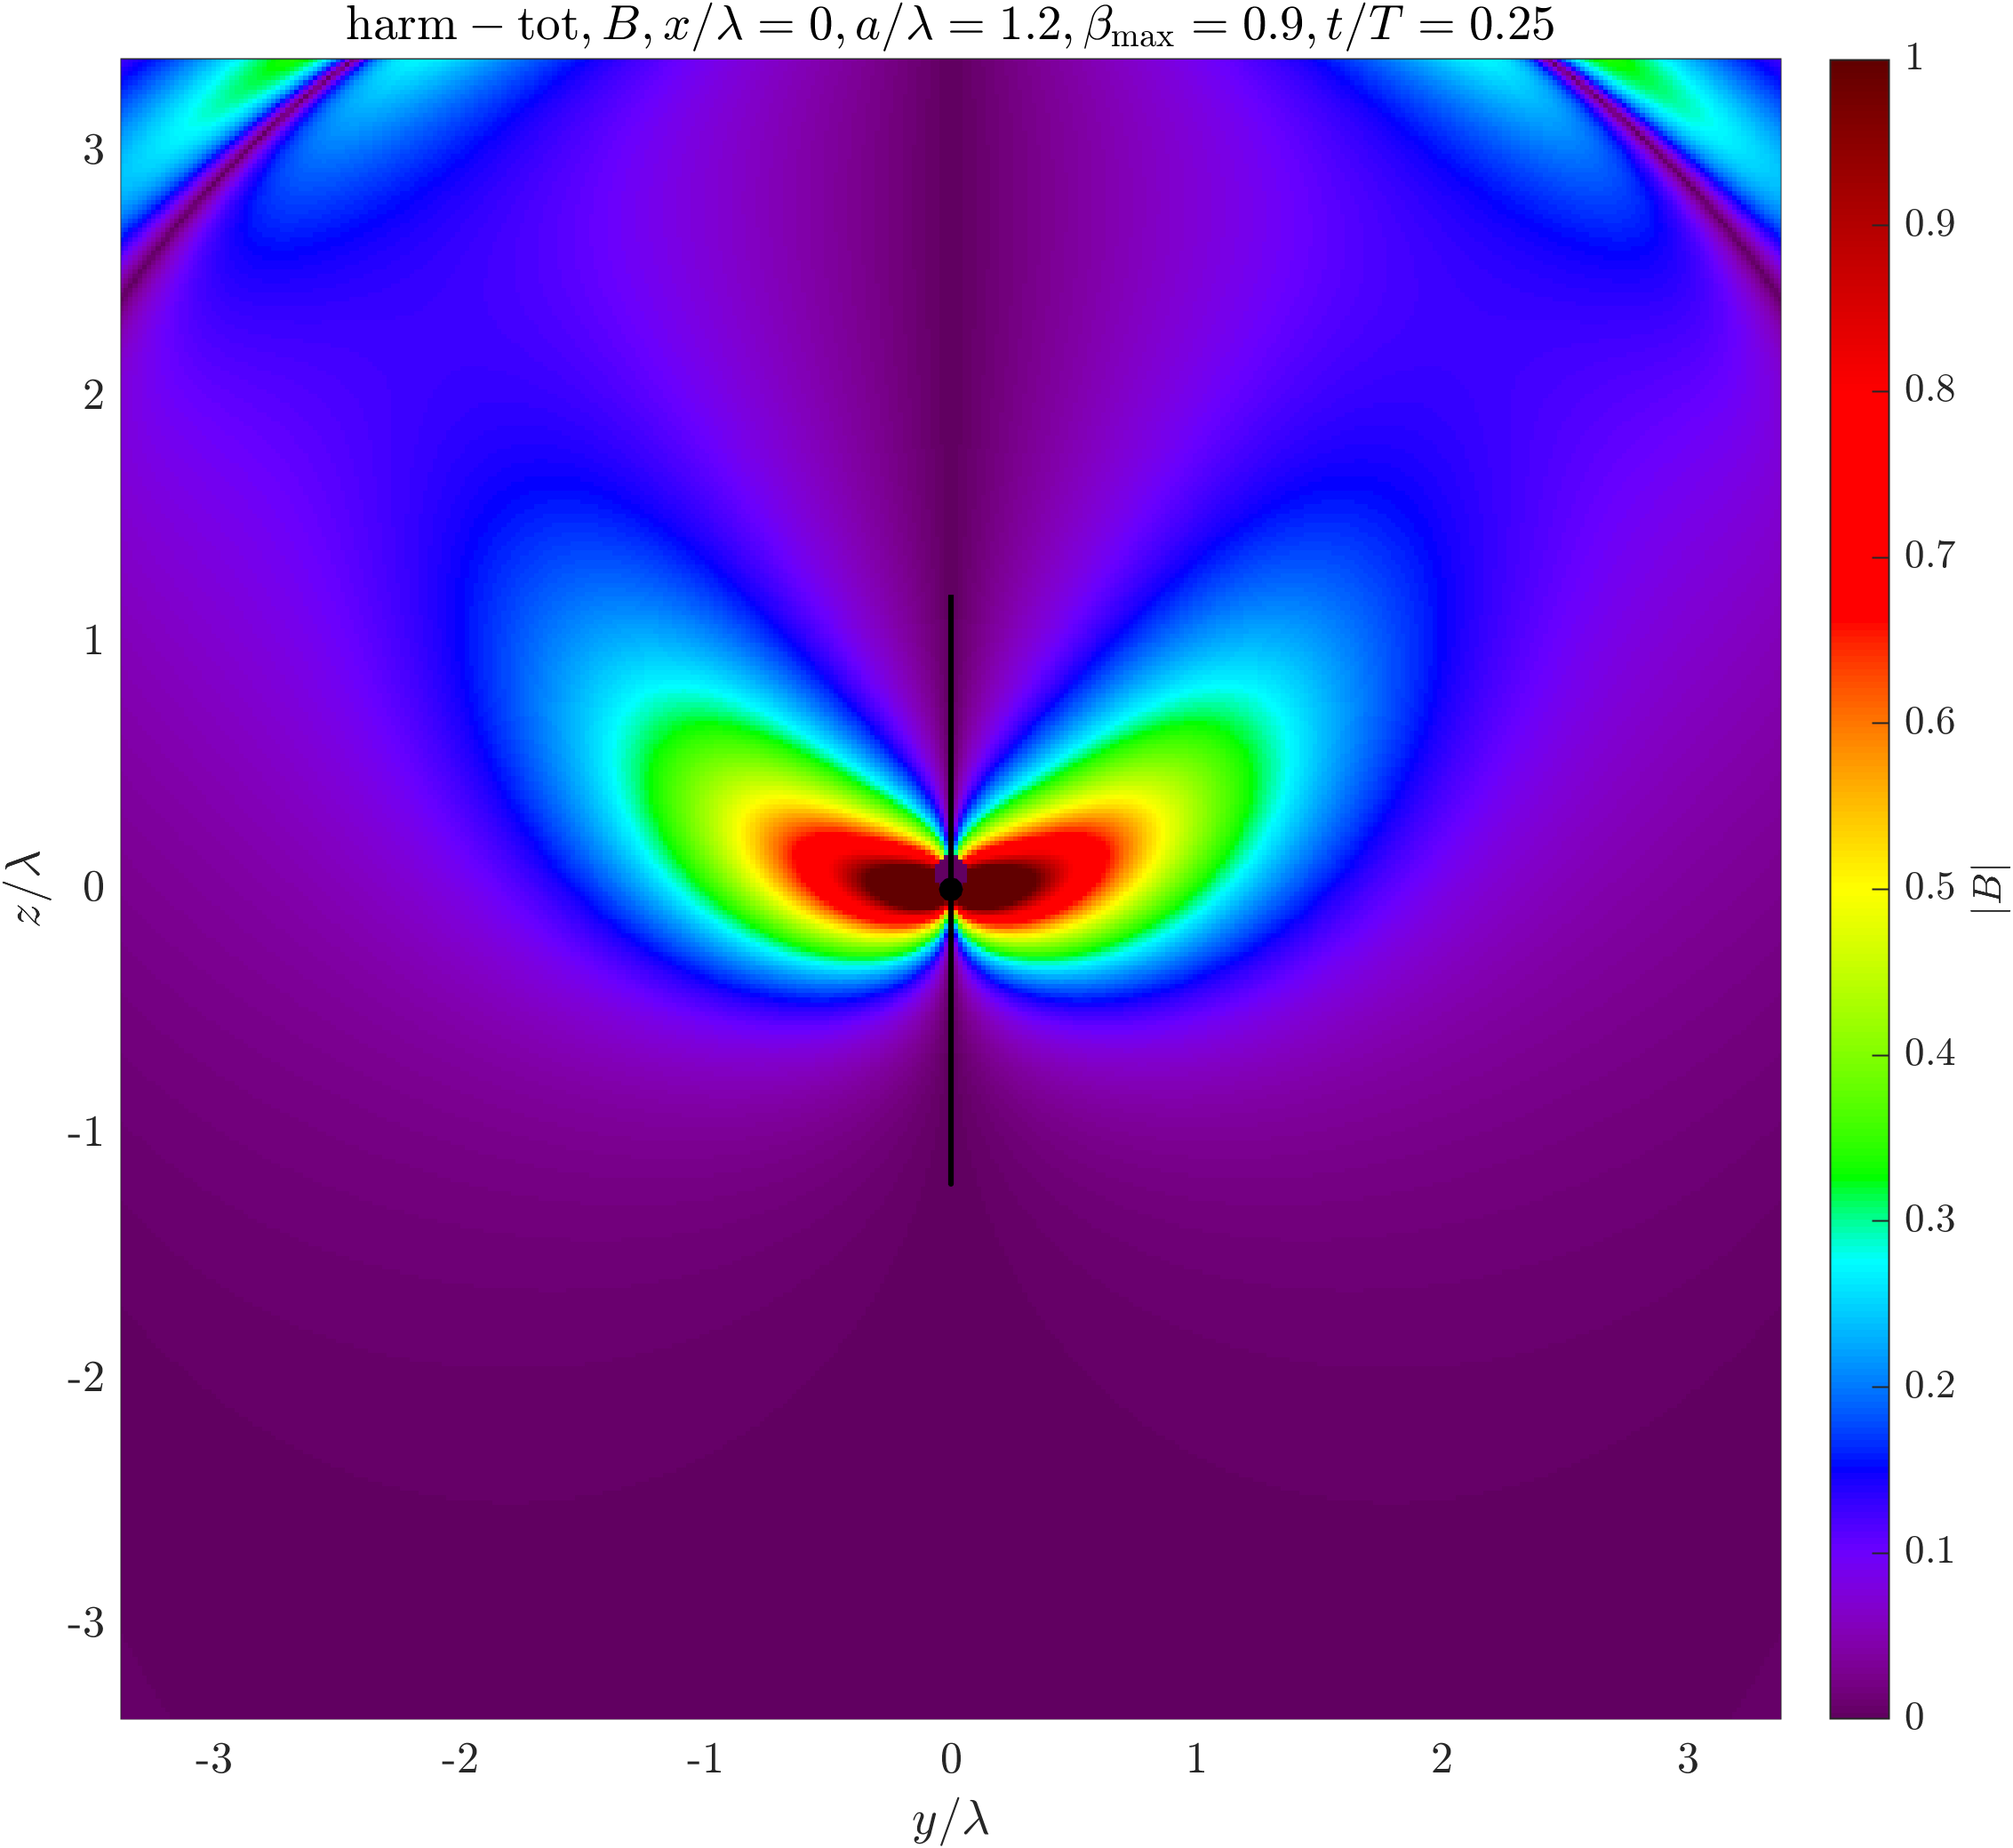
\includegraphics[width=\textwidth]{radiation_fig/harmonic_motion_b_yz_beta_0_9_eta_0_25.png}
		\caption{\(B|_{yz}\) (\(\beta=0.9\), \(\eta=0.25\))}
		\label{点电荷简谐运动辐射场示意图-B|_yz(beta=0.9,eta=0.25)}
	\end{subfigure}
	\vspace{0.2cm}
	\begin{subfigure}[b]{0.23\textwidth}
		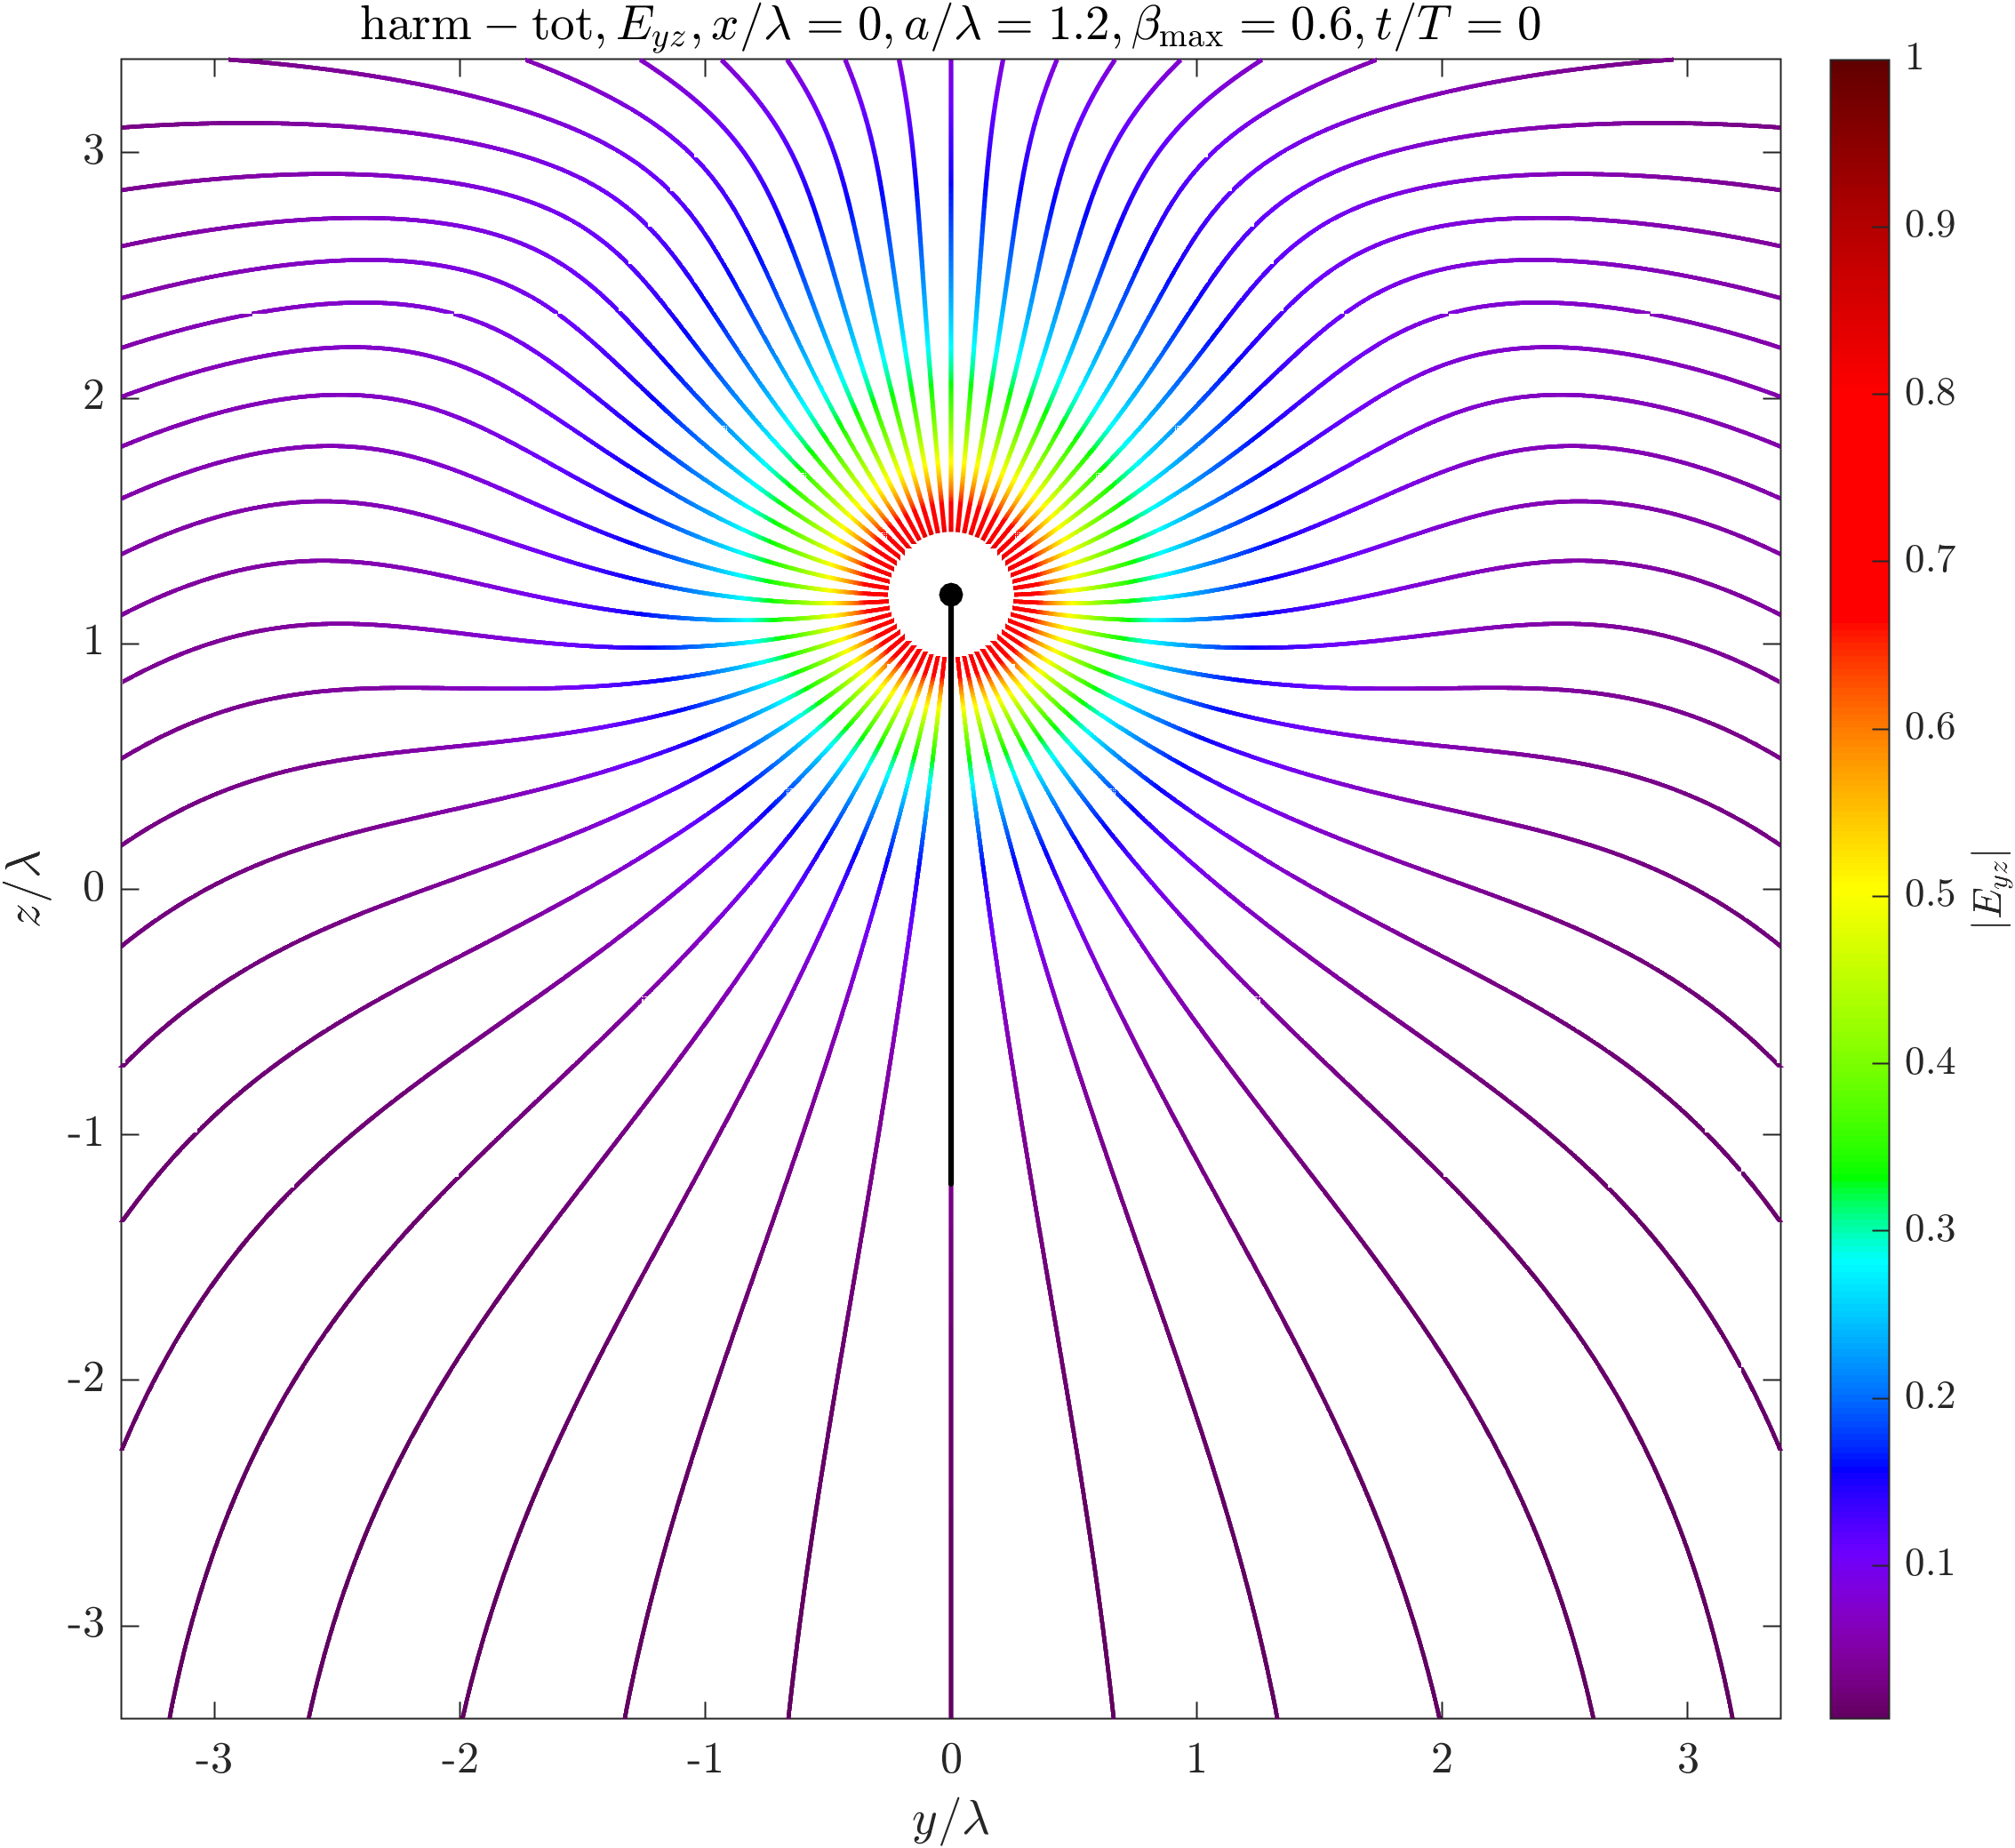
\includegraphics[width=\textwidth]{radiation_fig/harmonic_motion_e_farfield_yz_beta_0_6_eta_0.png}
		\caption{\(E|_{yz}\) (\(\beta=0.6\), \(\eta=0\))}
		\label{点电荷简谐运动辐射场示意图-E|_yz(beta=0.6,eta=0)-2}
	\end{subfigure}
	\hfill
	\begin{subfigure}[b]{0.23\textwidth}
		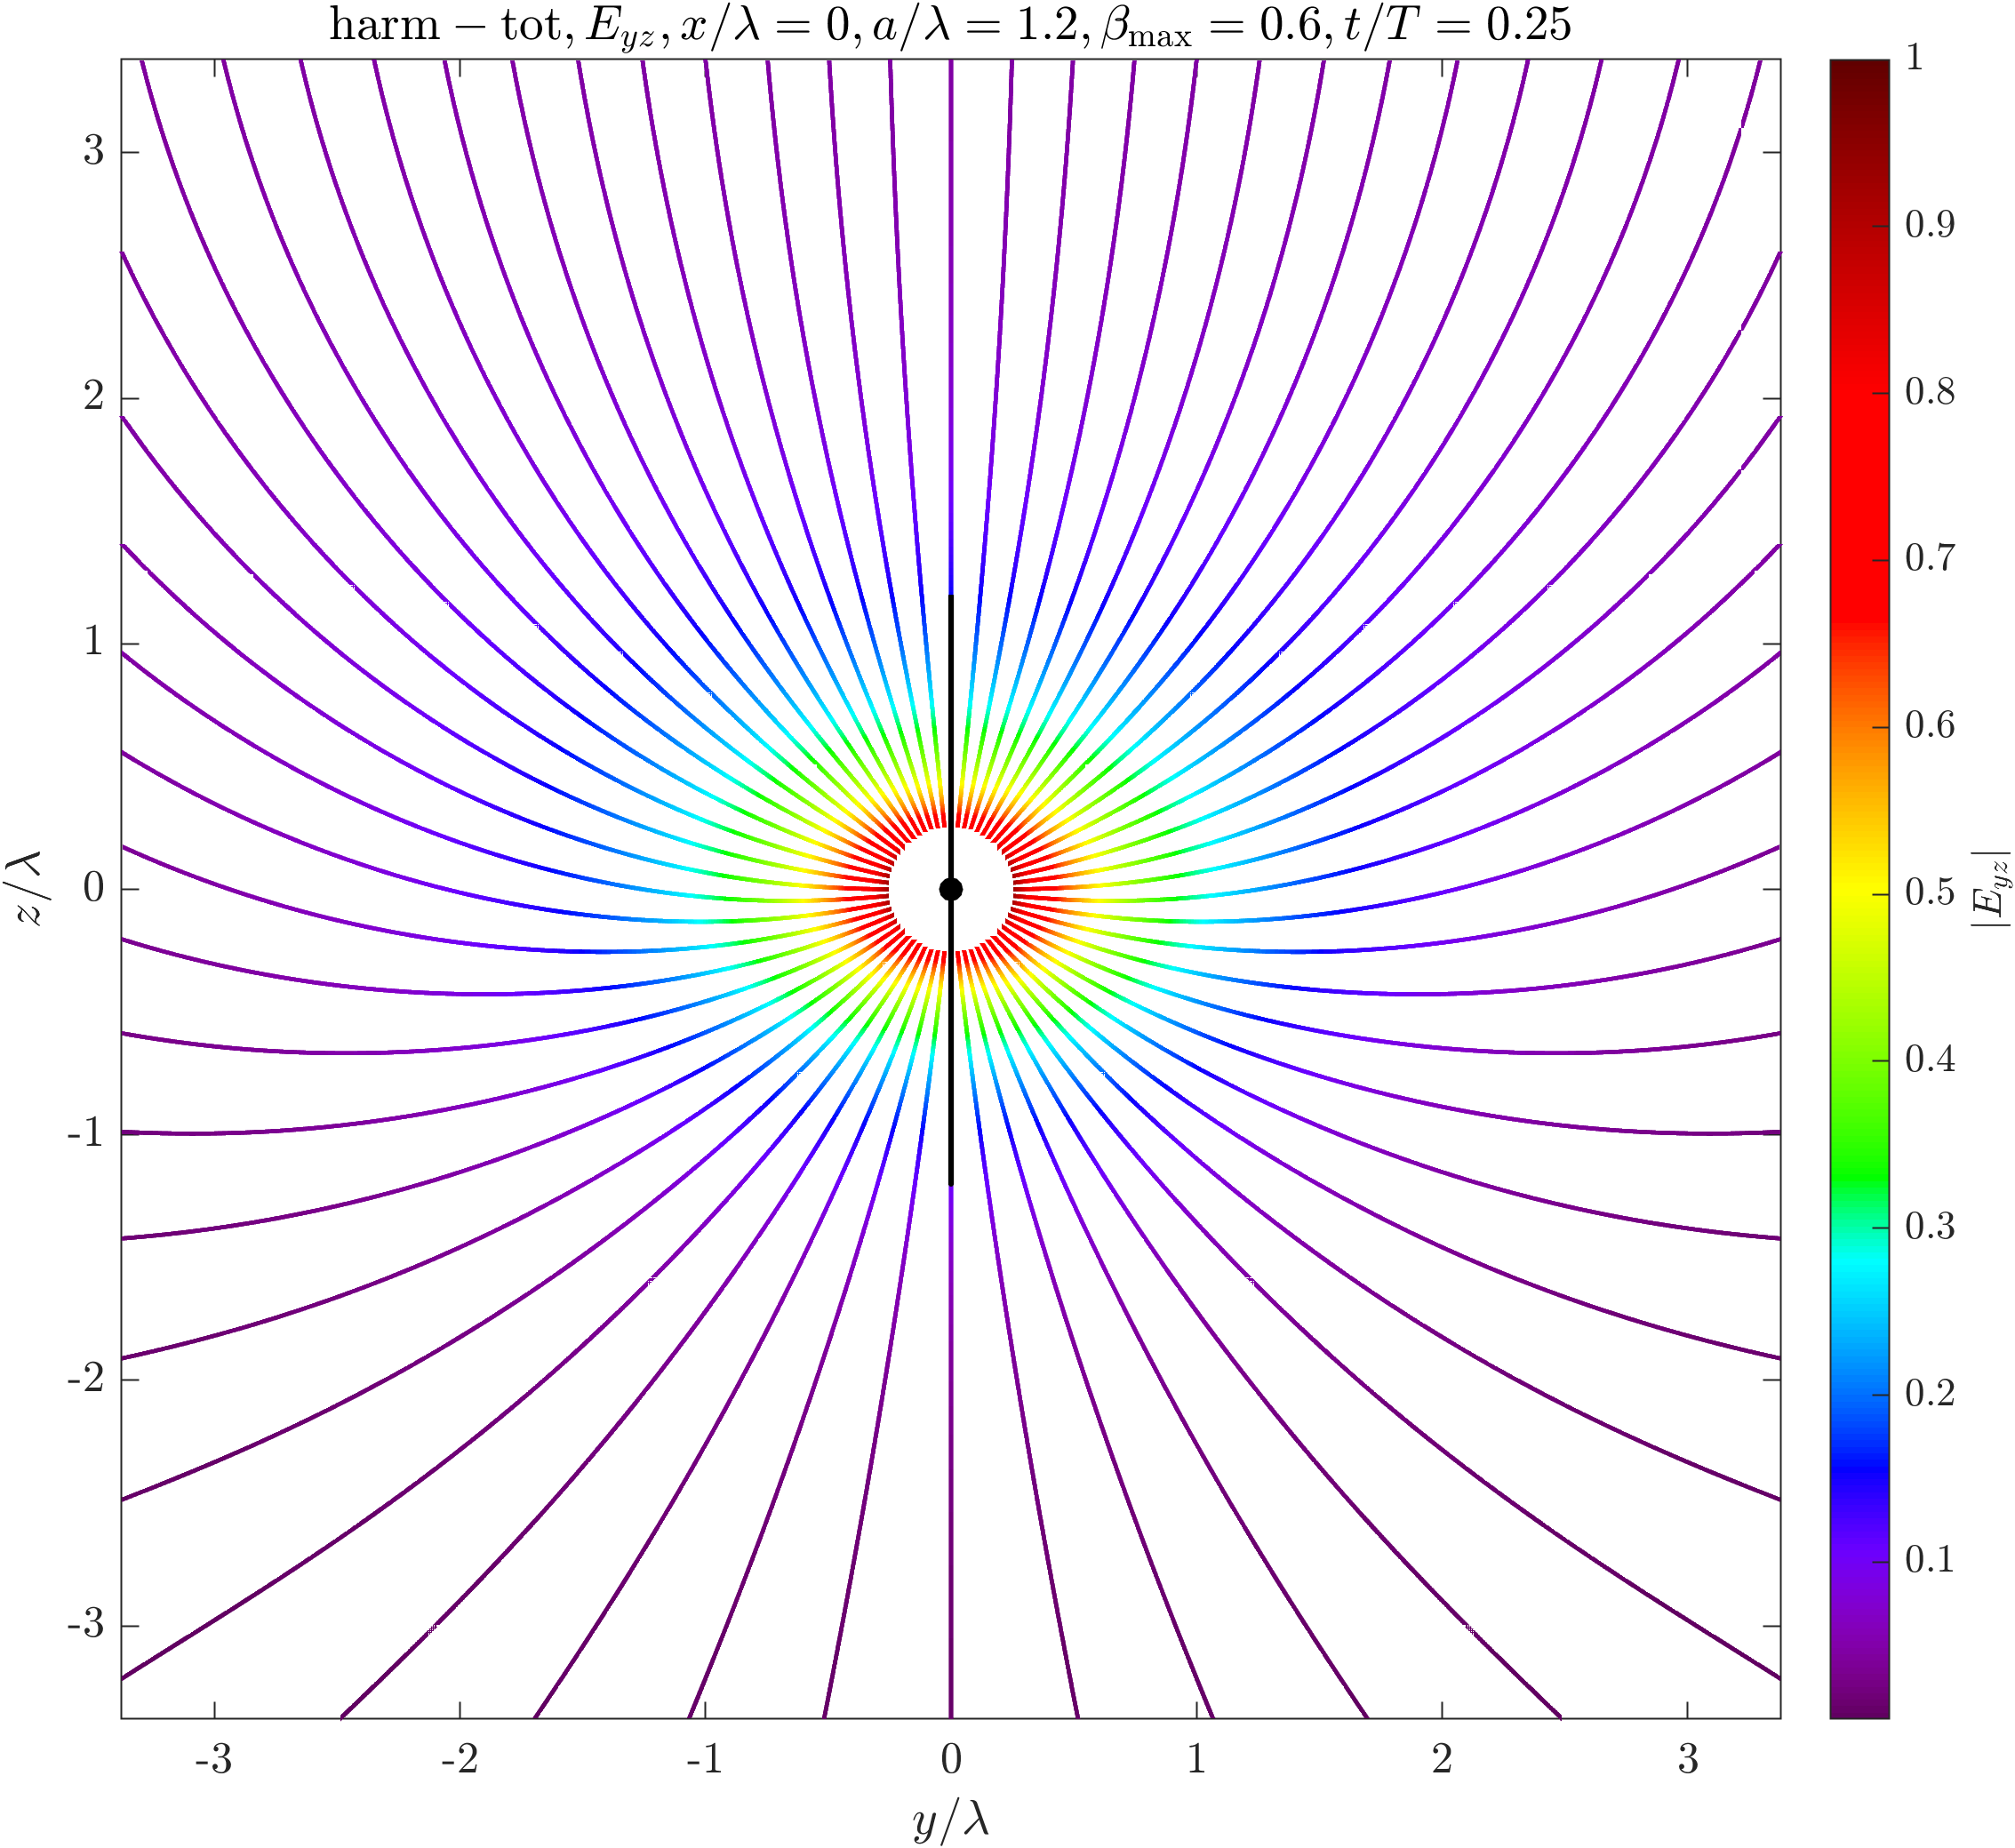
\includegraphics[width=\textwidth]{radiation_fig/harmonic_motion_e_farfield_yz_beta_0_6_eta_0_25.png}
		\caption{\(E|_{yz}\) (\(\beta=0.6\), \(\eta=0.25\))}
		\label{点电荷简谐运动辐射场示意图-E|_yz(beta=0.6,eta=0.25)-2}
	\end{subfigure}
	\hfill
	\begin{subfigure}[b]{0.23\textwidth}
		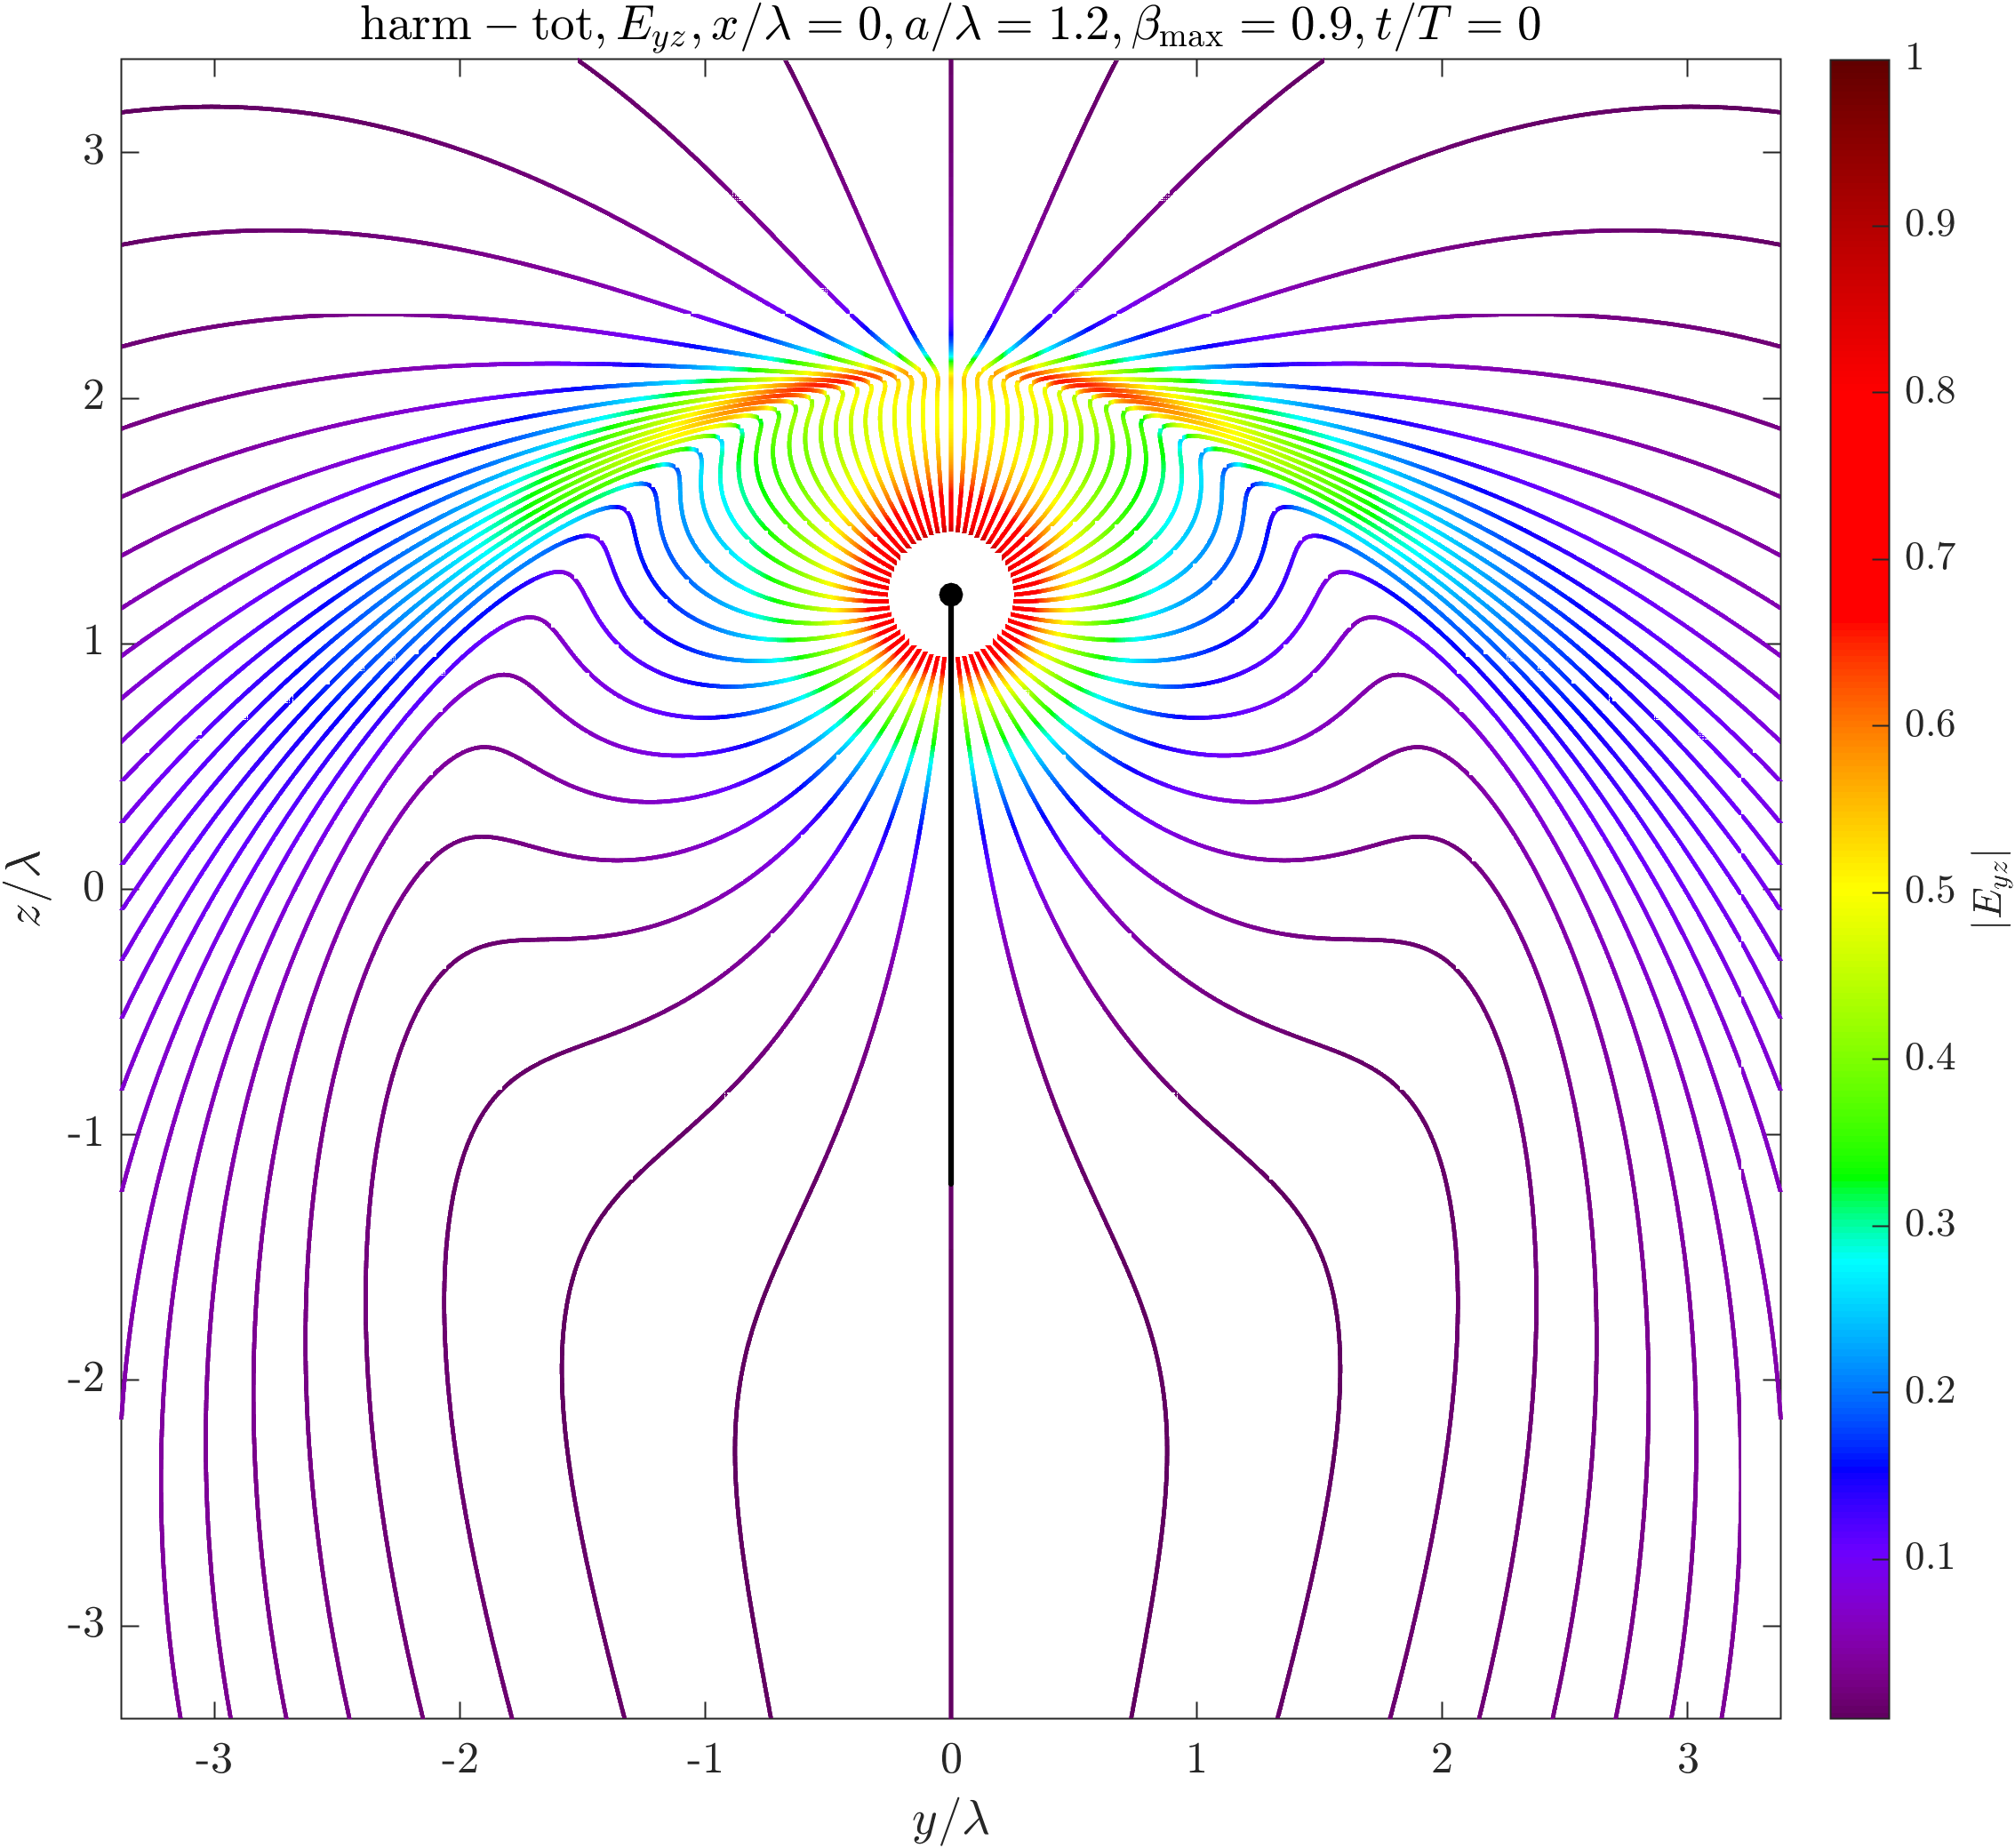
\includegraphics[width=\textwidth]{radiation_fig/harmonic_motion_e_farfield_yz_beta_0_9_eta_0.png}
		\caption{\(E|_{yz}\) (\(\beta=0.9\), \(\eta=0\))}
		\label{点电荷简谐运动辐射场示意图-E|_yz(beta=0.9,eta=0)-2}
	\end{subfigure}
	\hfill
	\begin{subfigure}[b]{0.23\textwidth}
		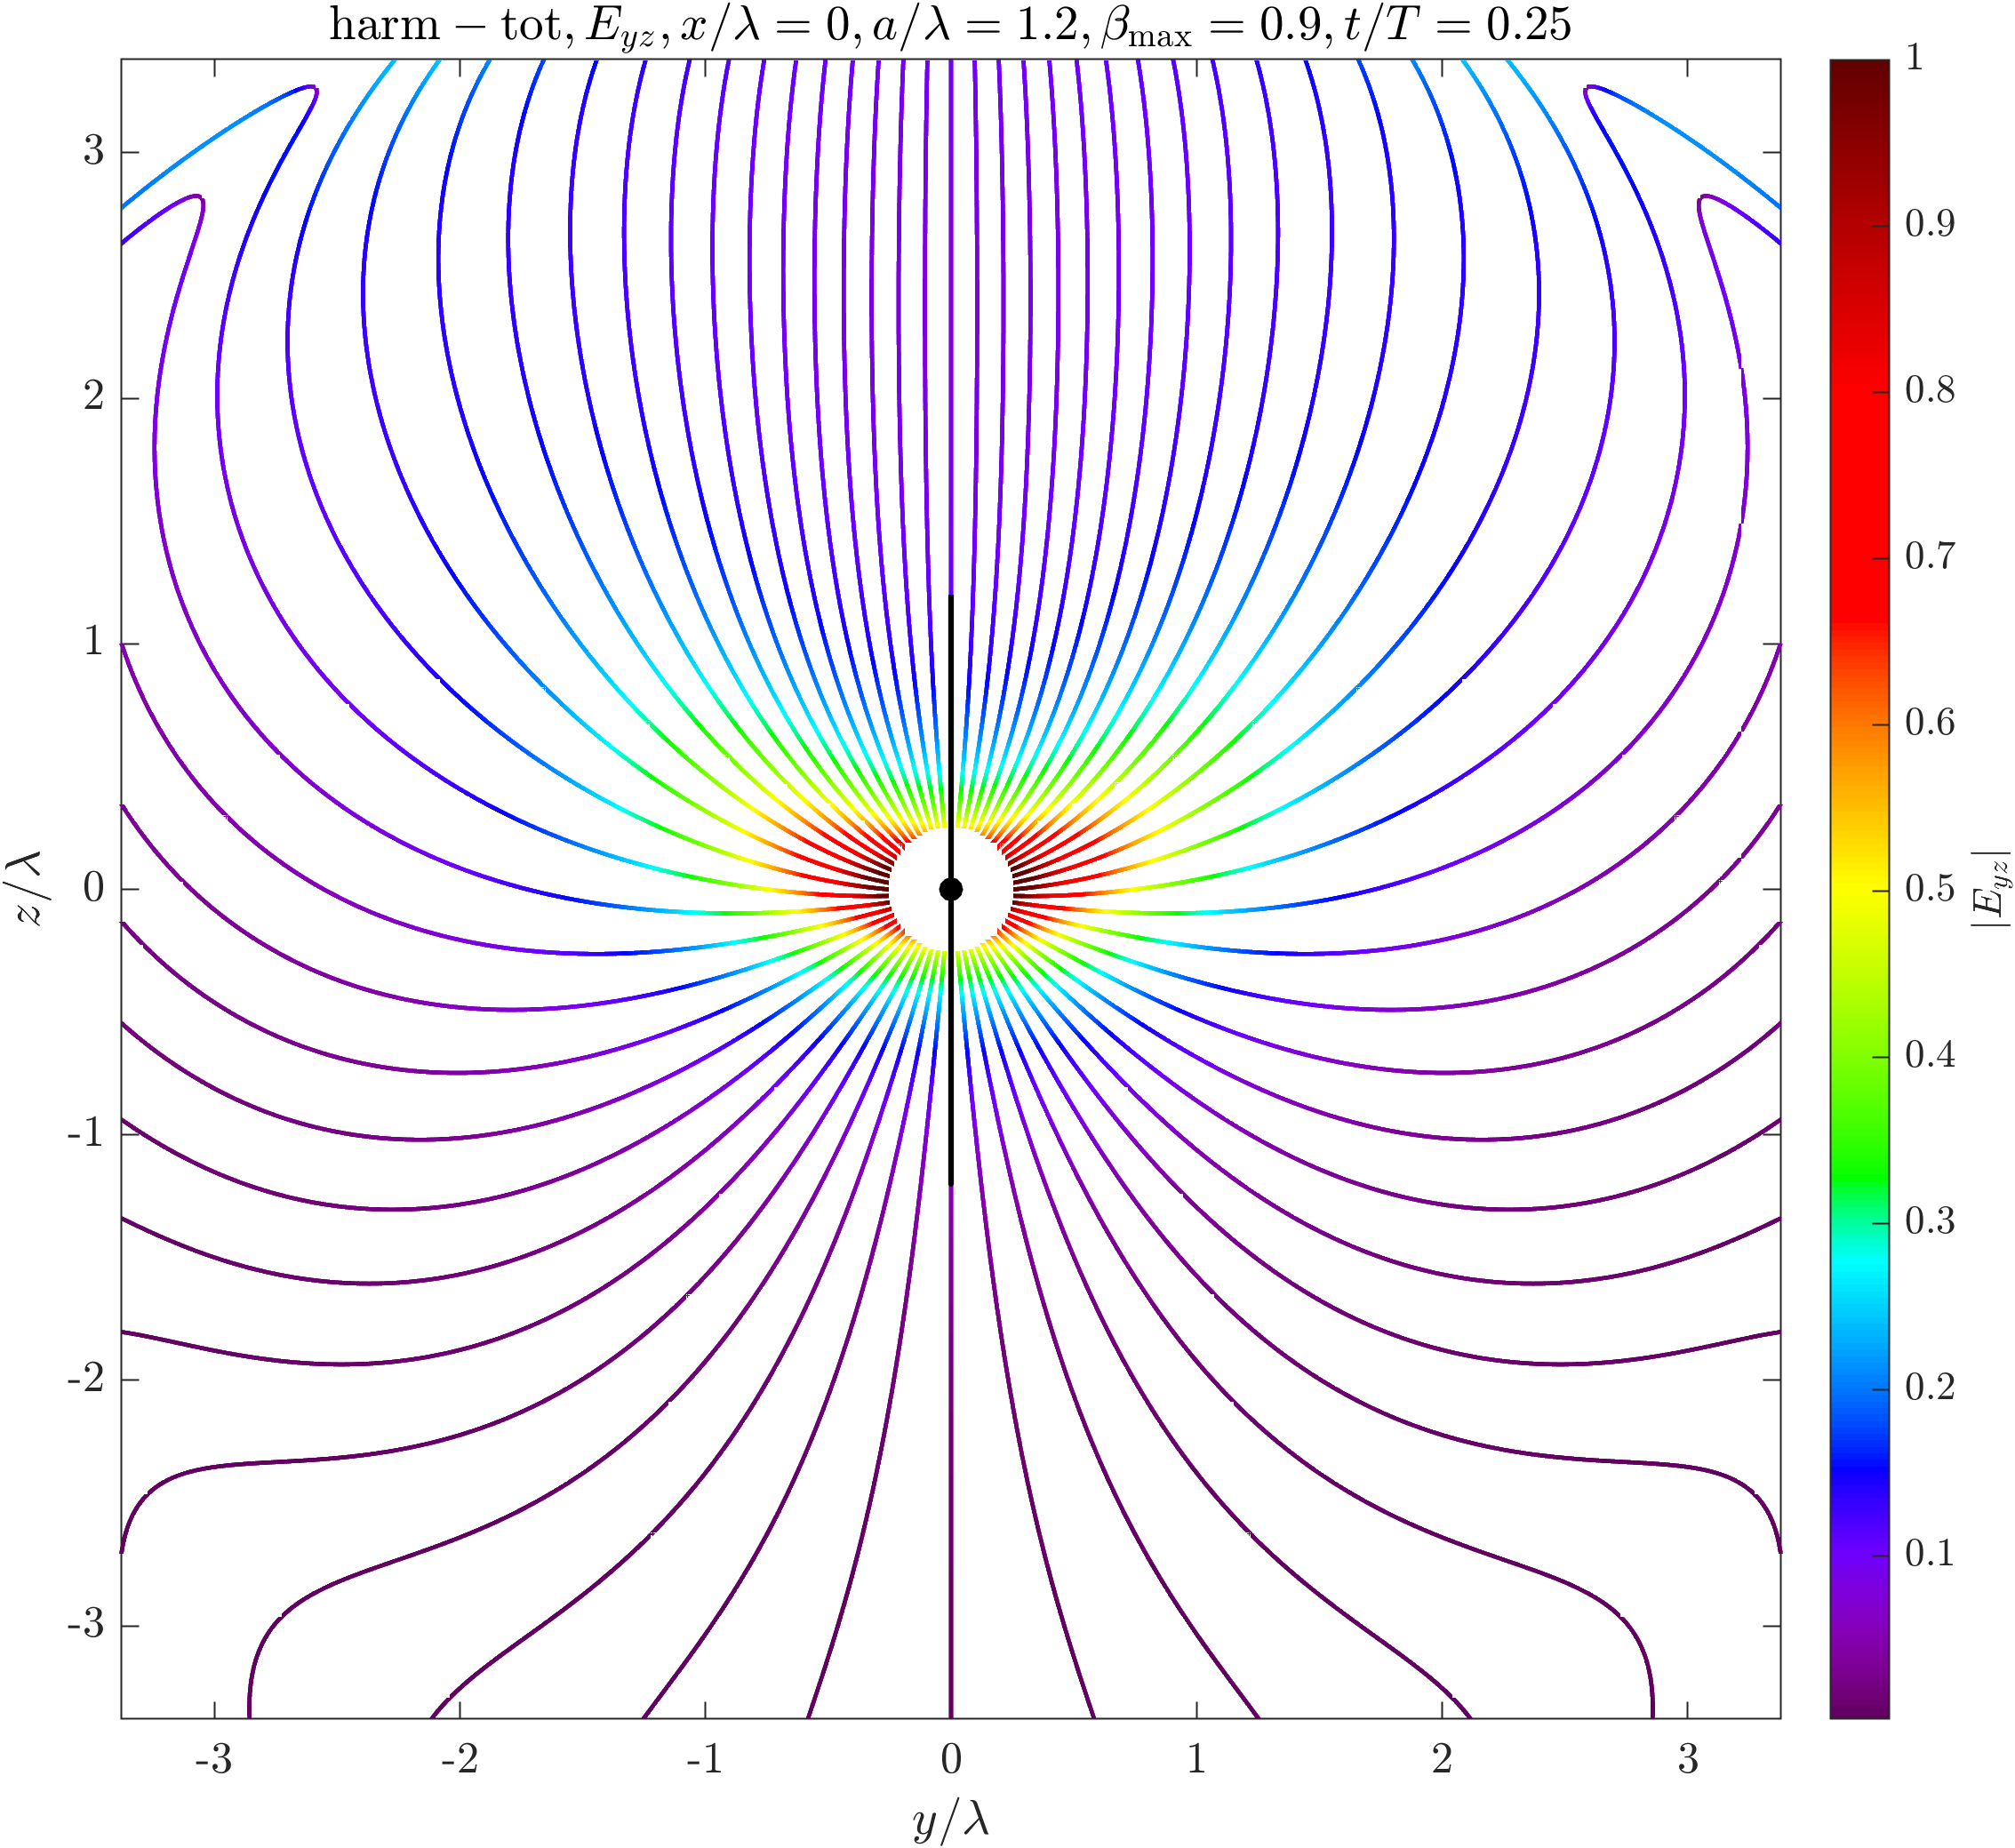
\includegraphics[width=\textwidth]{radiation_fig/harmonic_motion_e_farfield_yz_beta_0_9_eta_0_25.png}
		\caption{\(E|_{yz}\) (\(\beta=0.9\), \(\eta=0.25\))}
		\label{点电荷简谐运动辐射场示意图-E|_yz(beta=0.9,eta=0.25)-2}
	\end{subfigure}
	\vspace{0.2cm}
	\begin{subfigure}[b]{0.23\textwidth}
		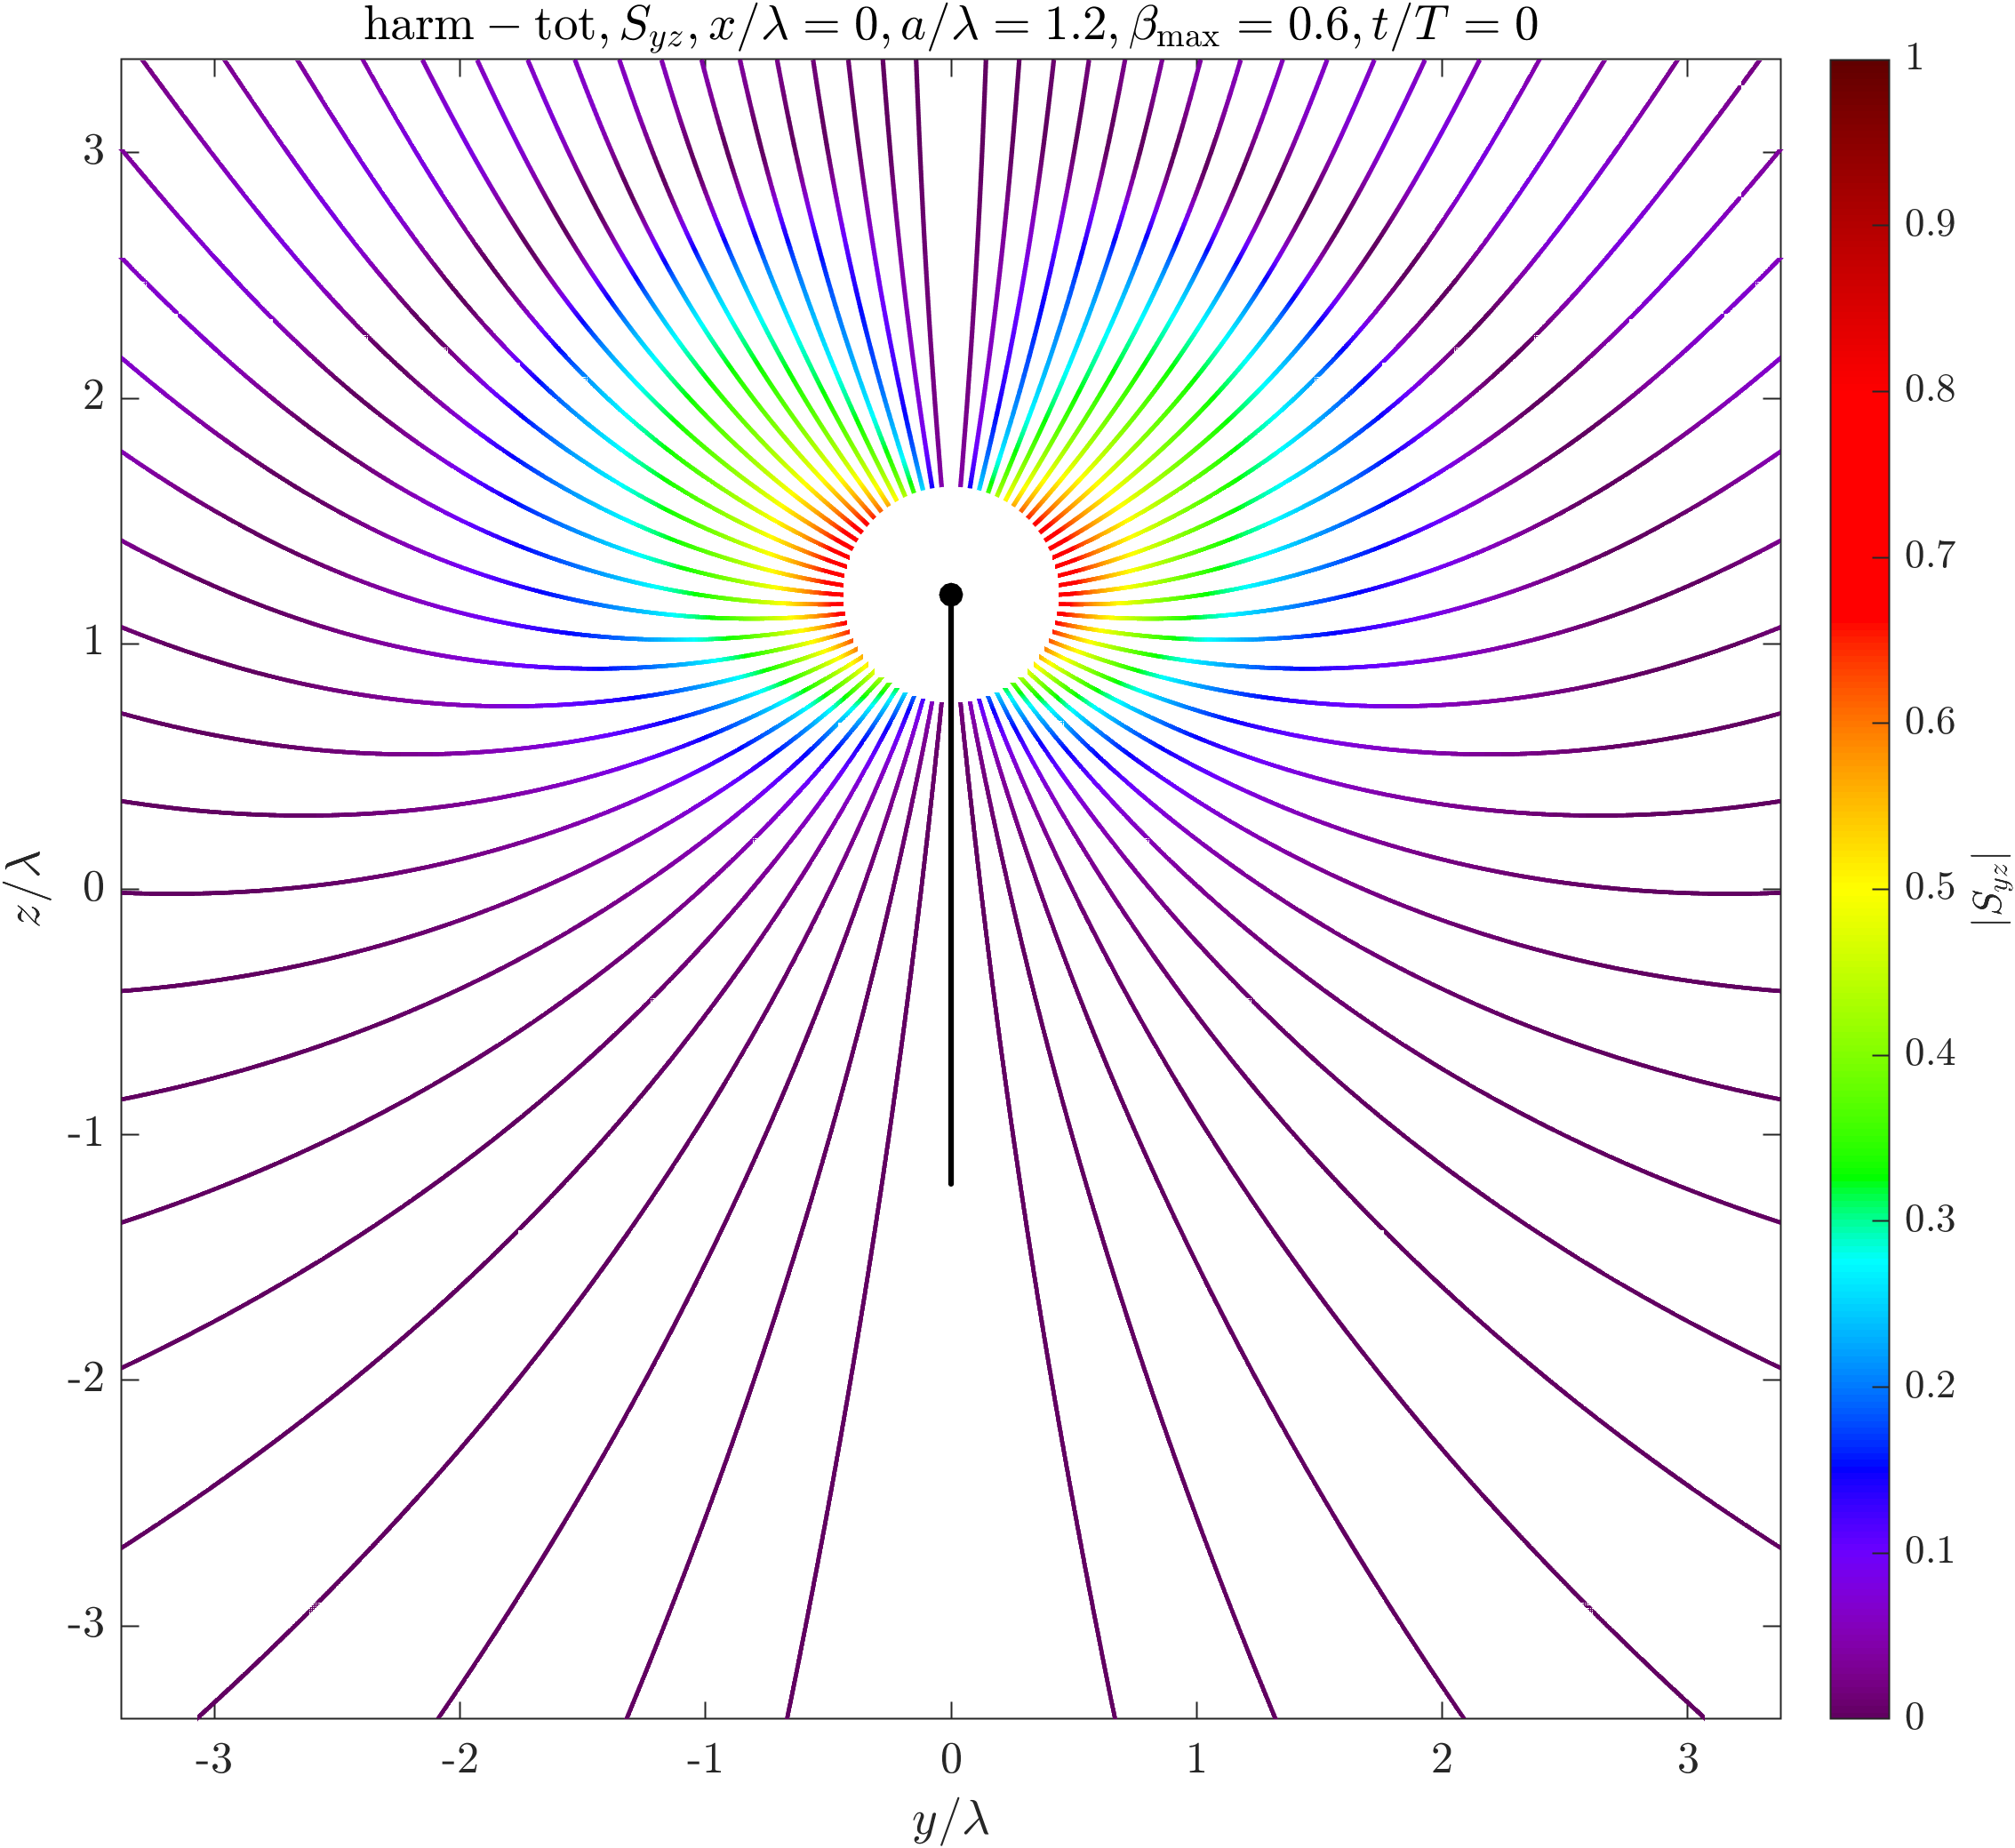
\includegraphics[width=\textwidth]{radiation_fig/harmonic_motion_s_yz_beta_0_6_eta_0.png}
		\caption{\(S|_{yz}\) (\(\beta=0.6\), \(\eta=0\))}
		\label{点电荷简谐运动辐射场示意图-S|_yz(beta=0.6,eta=0)}
	\end{subfigure}
	\hfill
	\begin{subfigure}[b]{0.23\textwidth}
		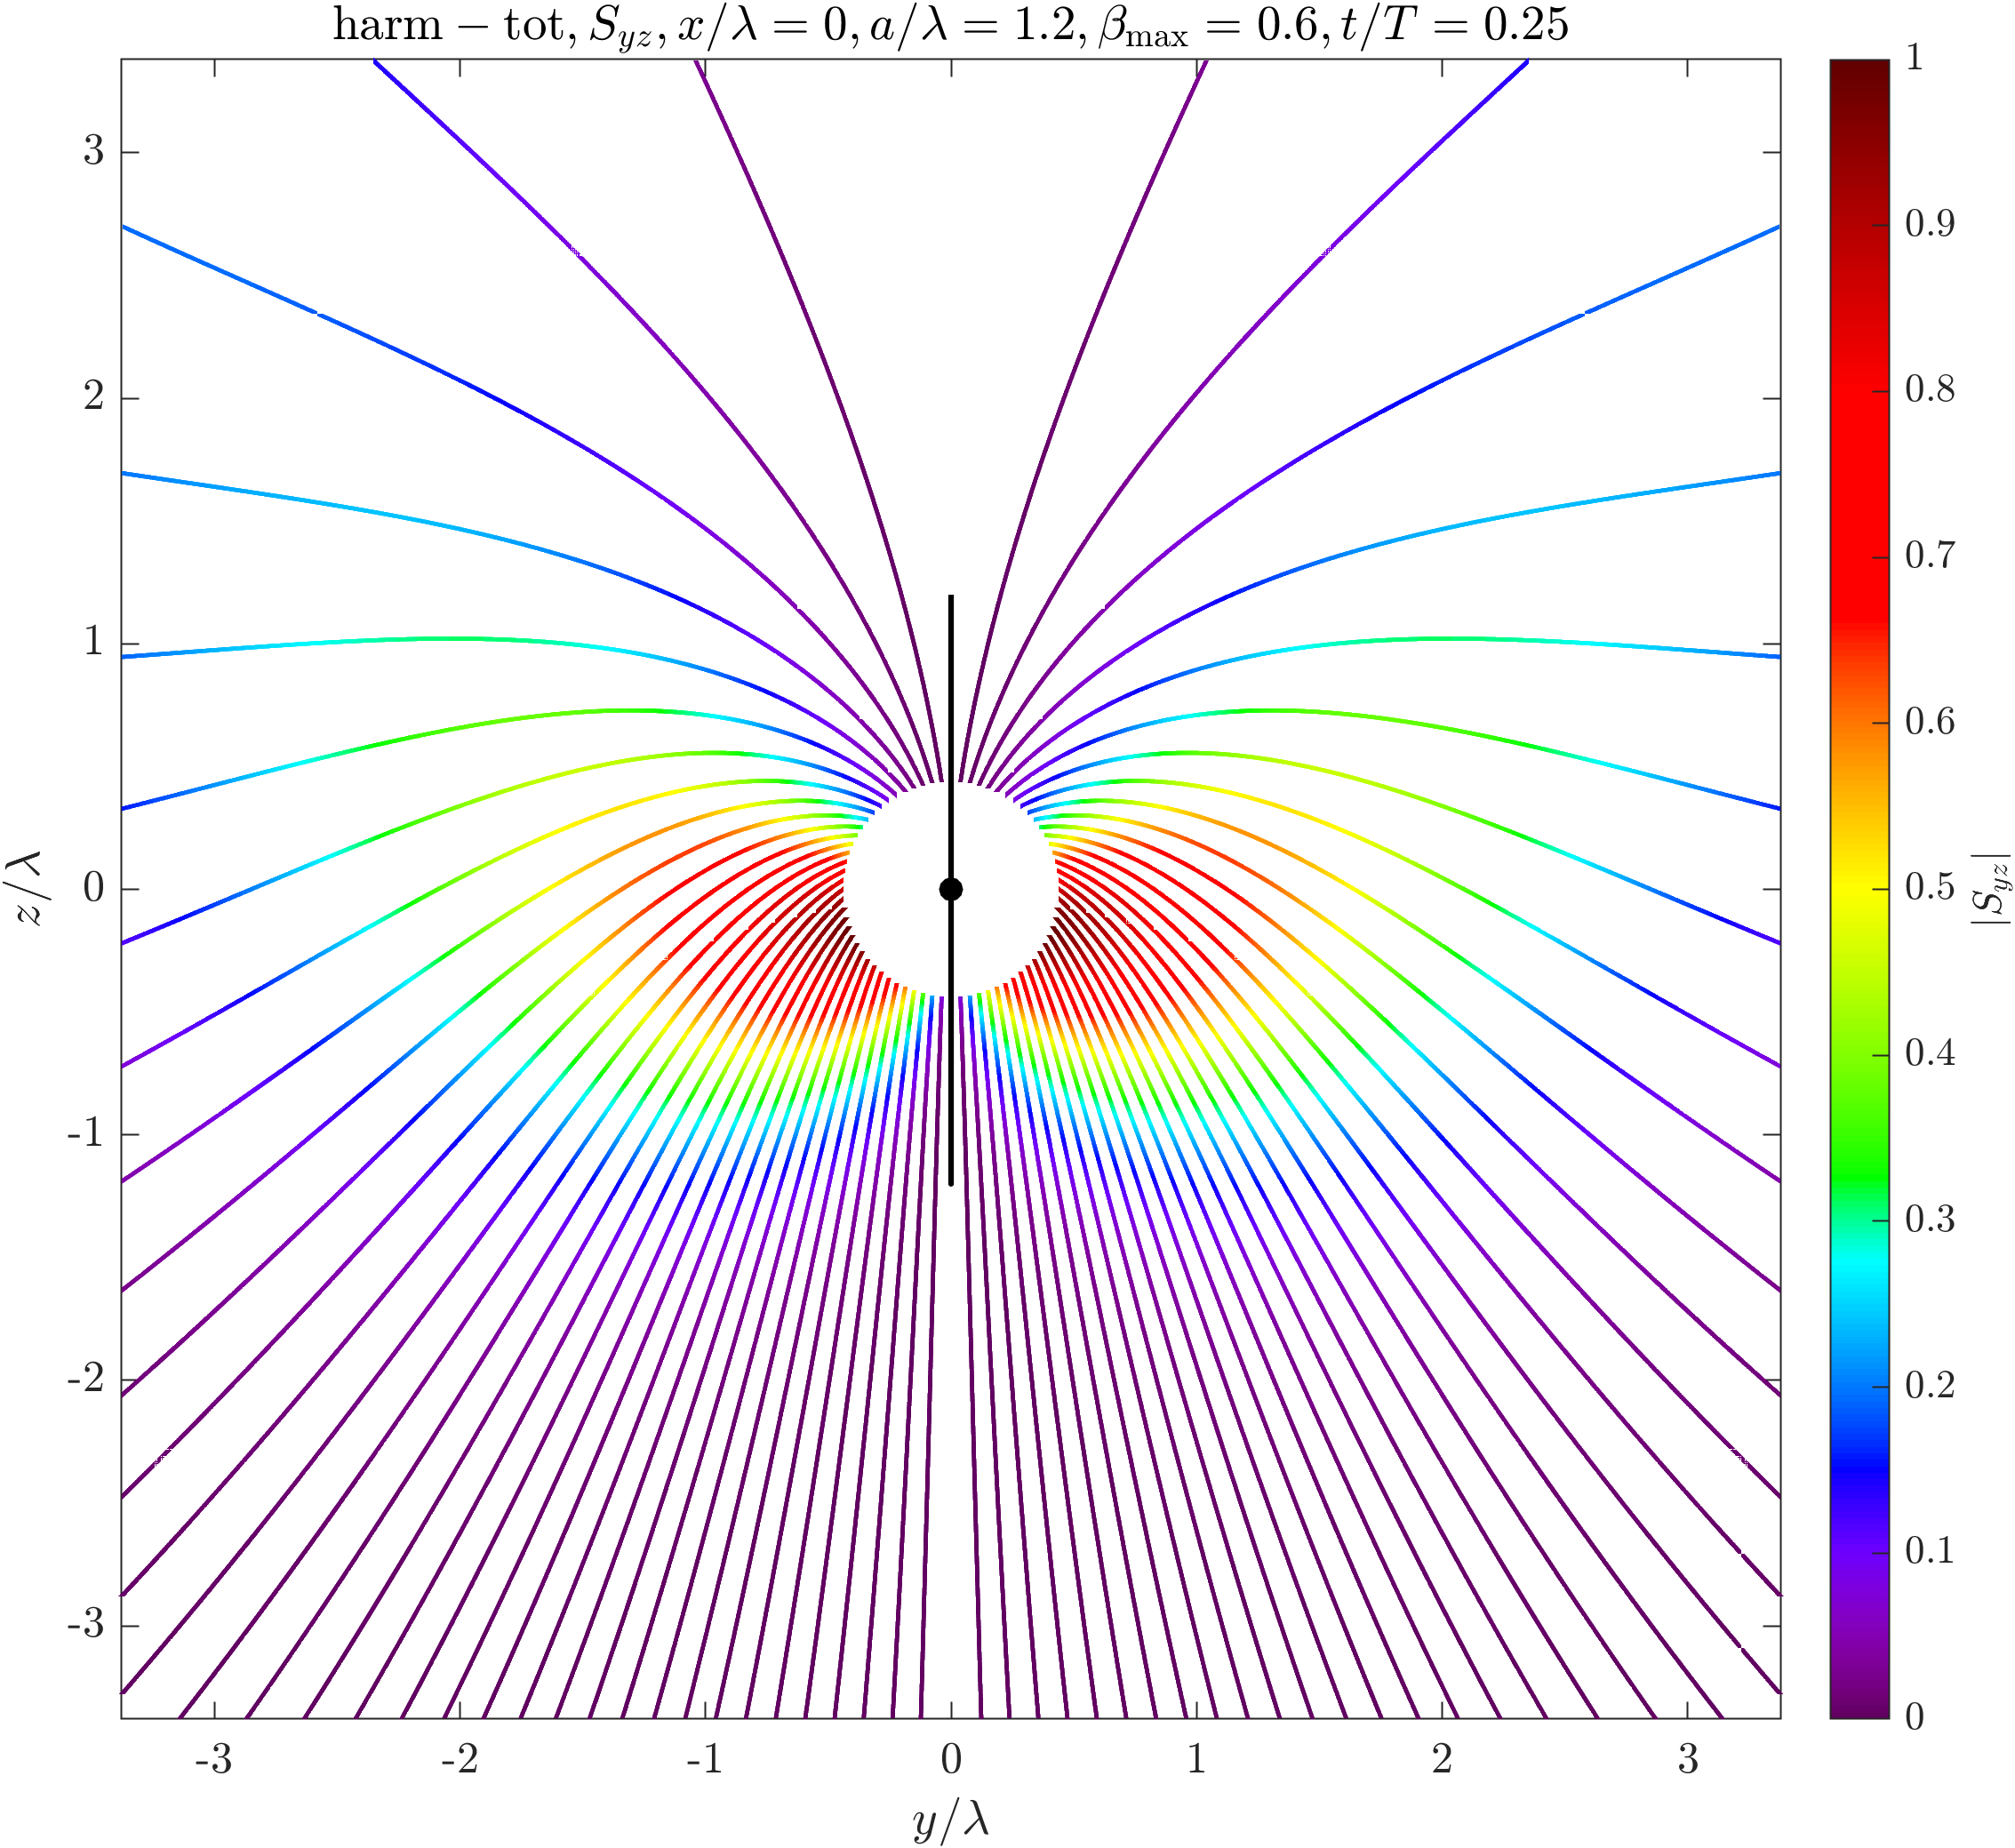
\includegraphics[width=\textwidth]{radiation_fig/harmonic_motion_s_yz_beta_0_6_eta_0_25.png}
		\caption{\(S|_{yz}\) (\(\beta=0.6\), \(\eta=0.25\))}
		\label{点电荷简谐运动辐射场示意图-S|_yz(beta=0.6,eta=0.25)}
	\end{subfigure}
	\hfill
	\begin{subfigure}[b]{0.23\textwidth}
		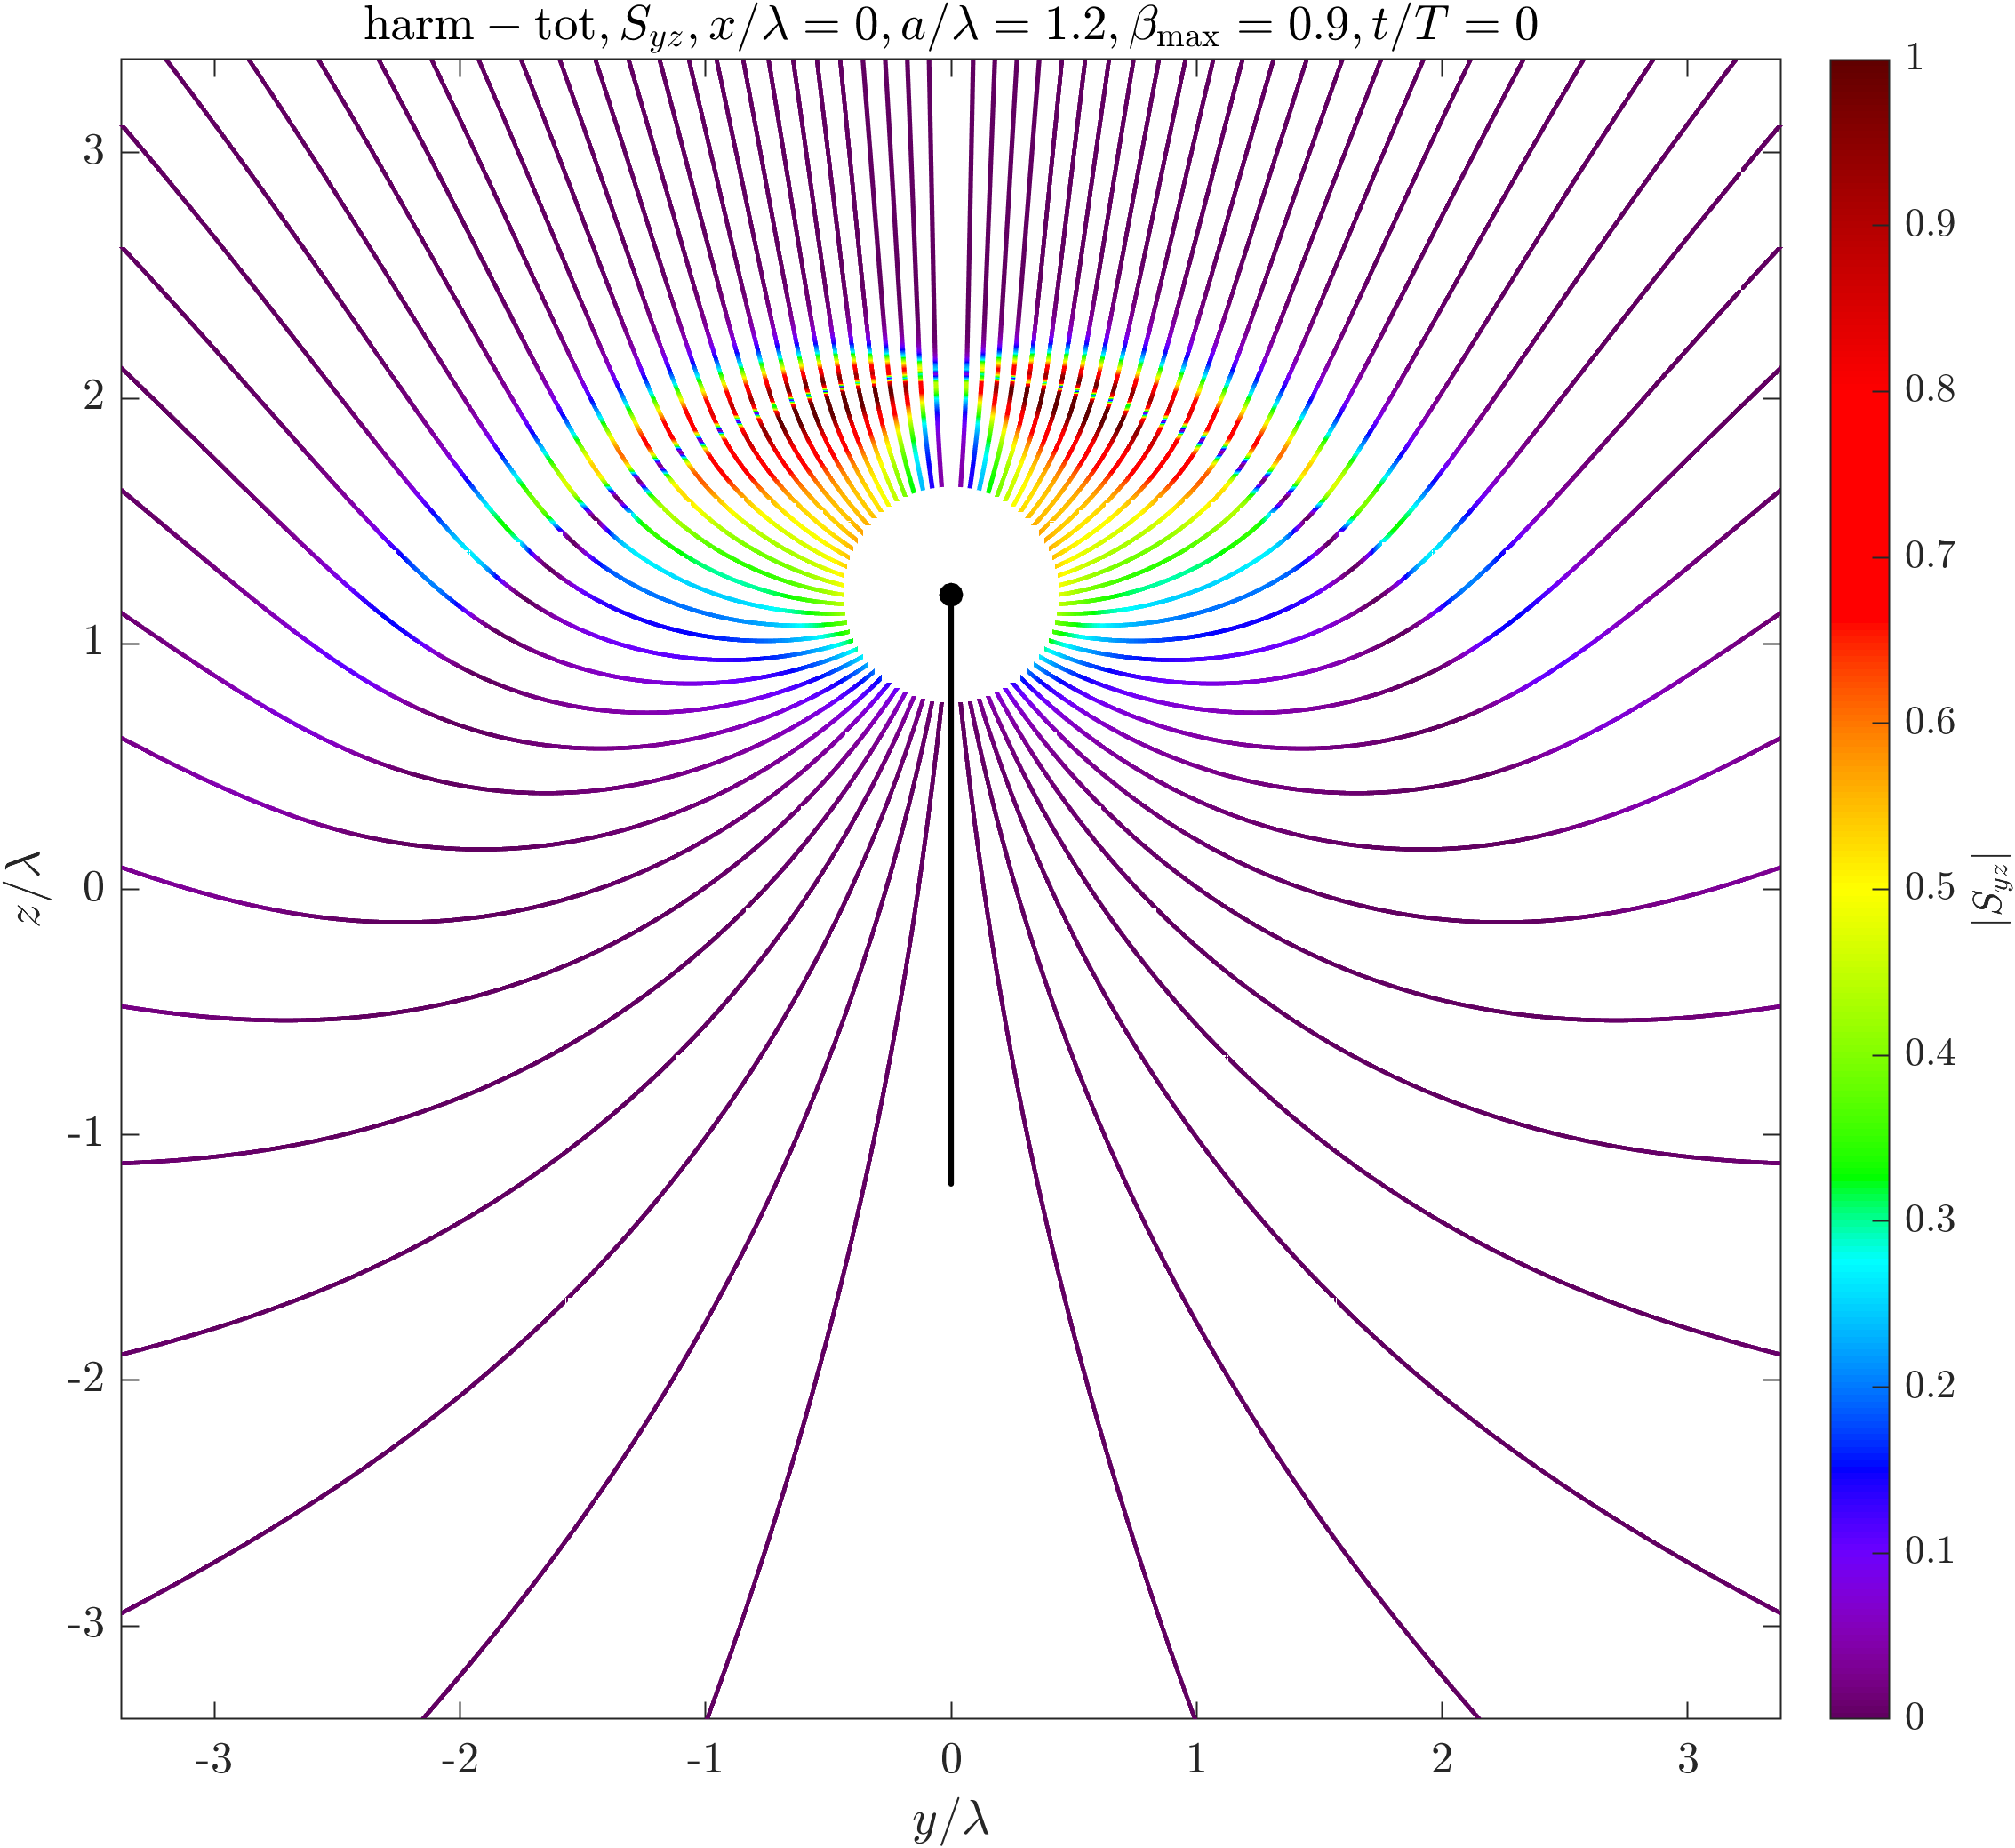
\includegraphics[width=\textwidth]{radiation_fig/harmonic_motion_s_yz_beta_0_9_eta_0.png}
		\caption{\(S|_{yz}\) (\(\beta=0.9\), \(\eta=0\))}
		\label{点电荷简谐运动辐射场示意图-S|_yz(beta=0.9,eta=0)}
	\end{subfigure}
	\hfill
	\begin{subfigure}[b]{0.23\textwidth}
		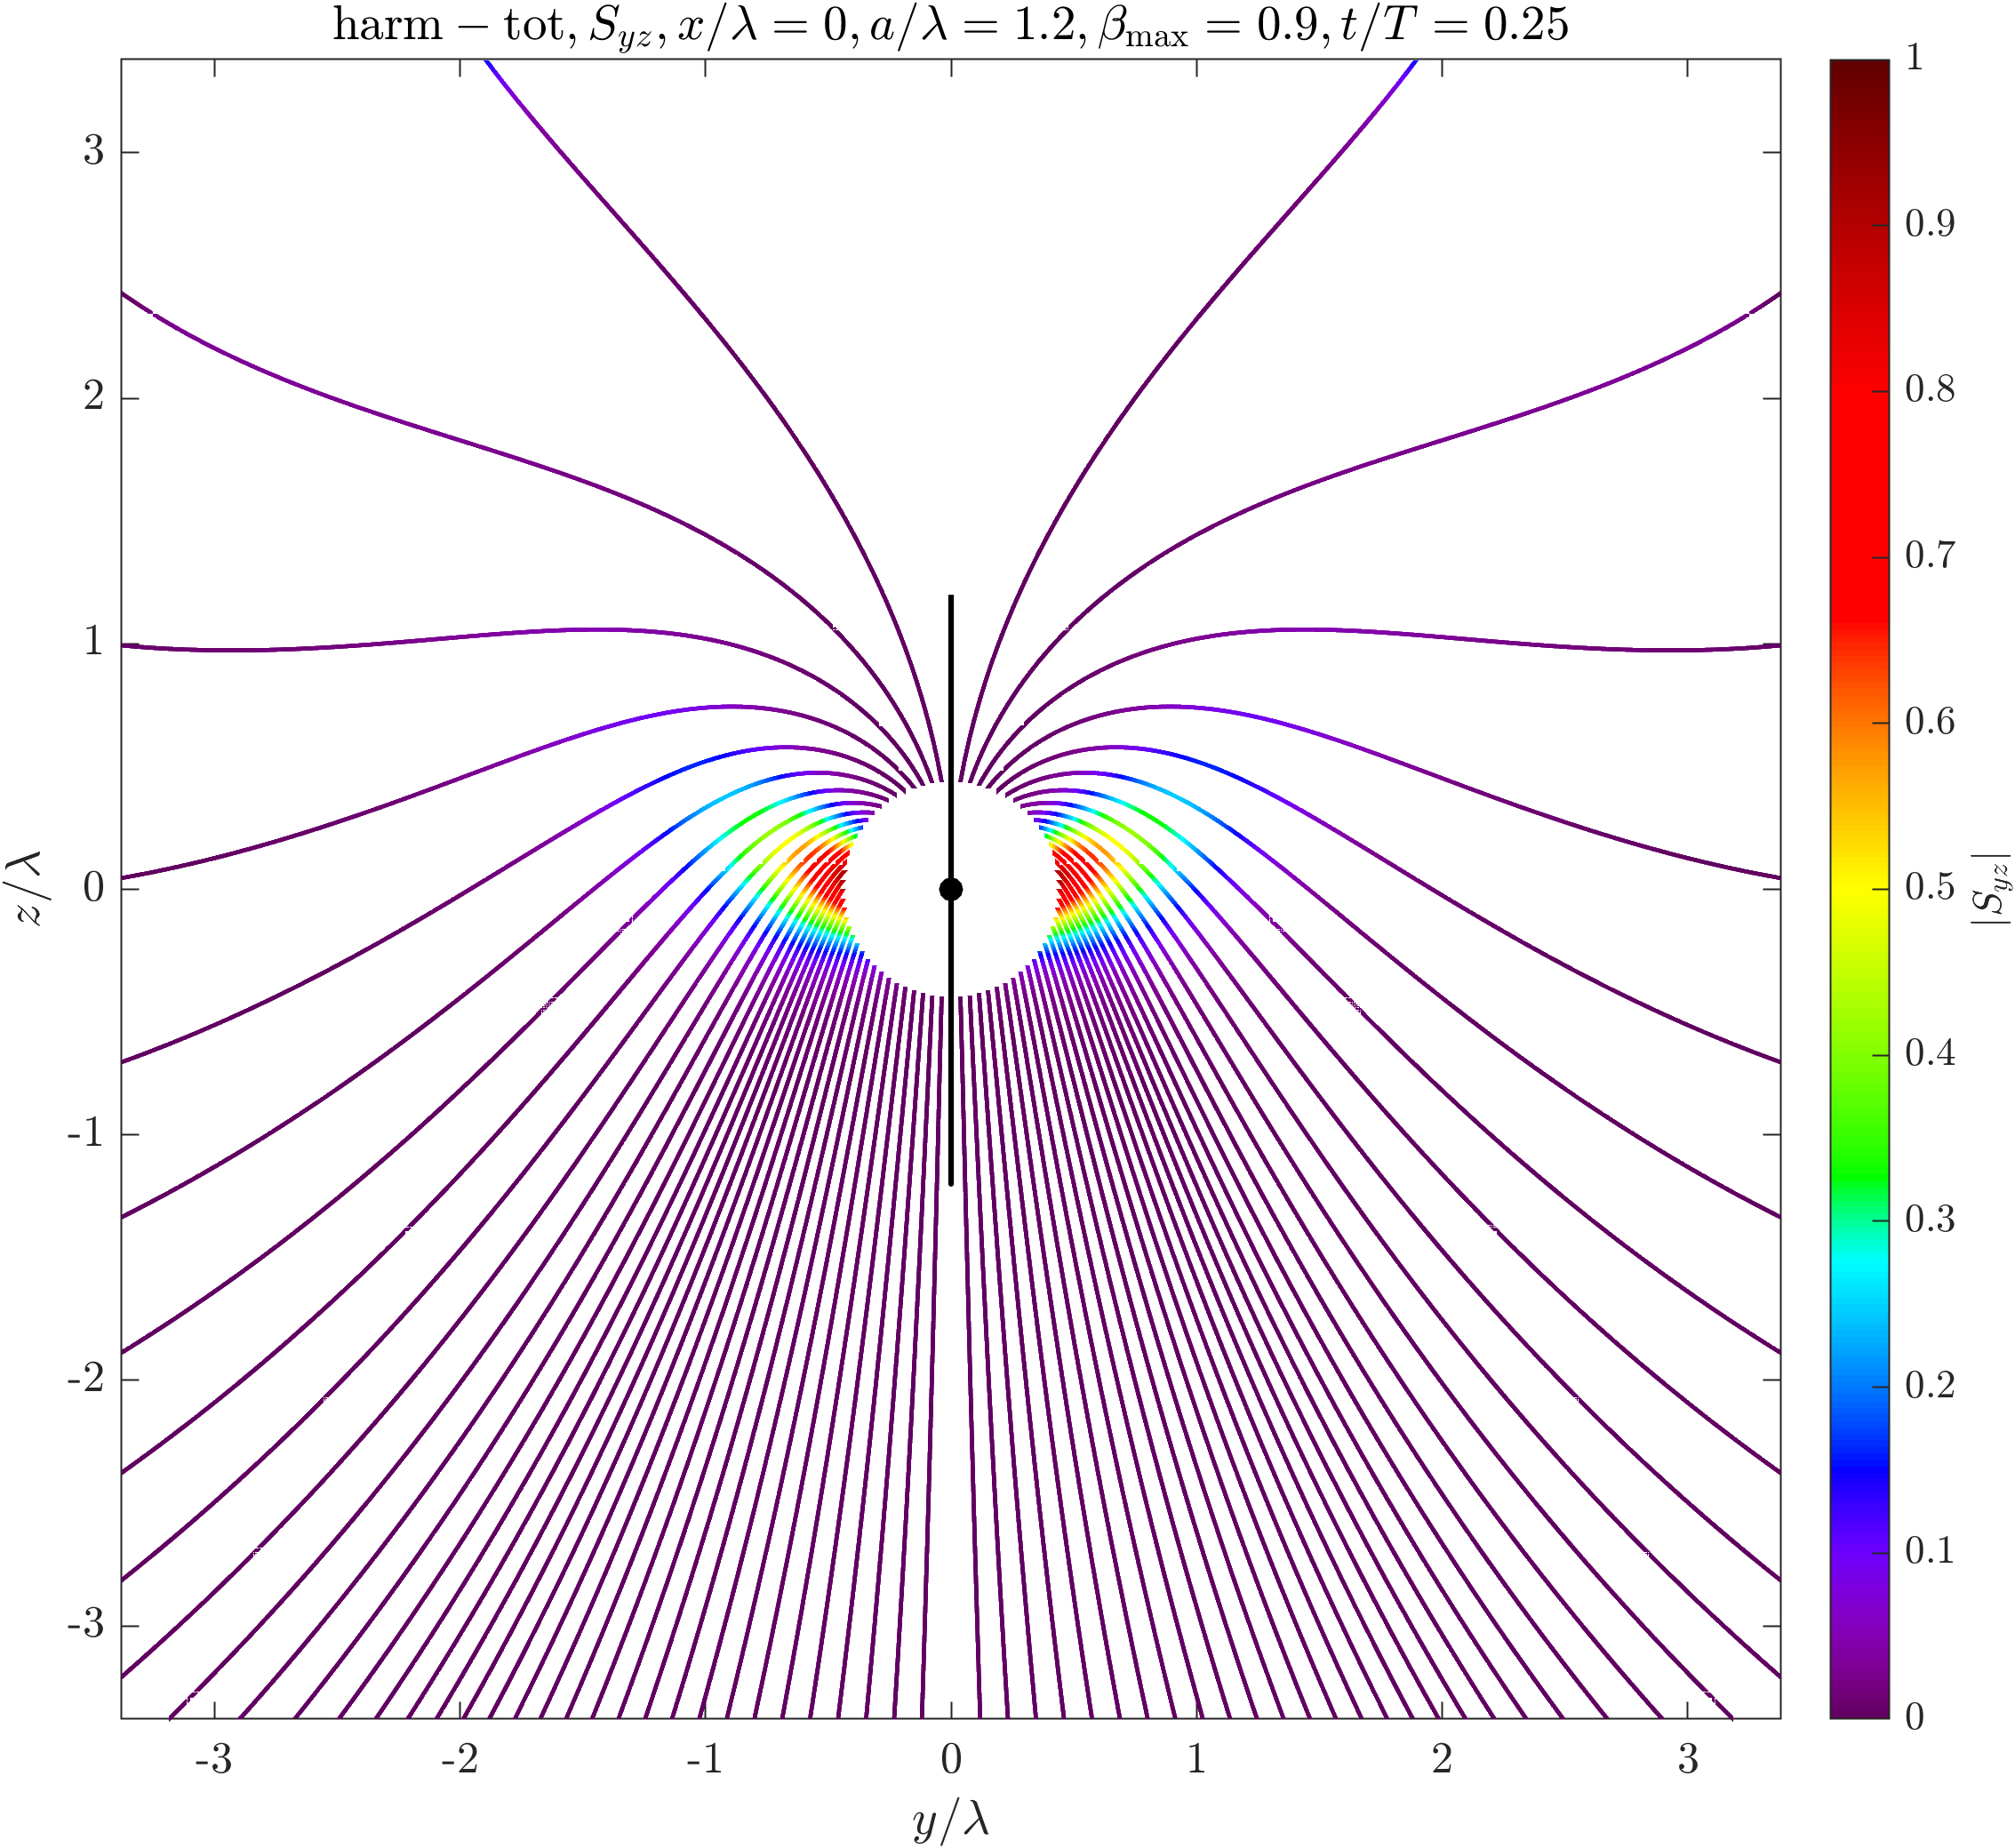
\includegraphics[width=\textwidth]{radiation_fig/harmonic_motion_s_yz_beta_0_9_eta_0_25.png}
		\caption{\(S|_{yz}\) (\(\beta=0.9\), \(\eta=0.25\))}
		\label{点电荷简谐运动辐射场示意图-S|_yz(beta=0.9,eta=0.25)}
	\end{subfigure}
	\vspace{0.2cm}
	\begin{subfigure}[b]{0.23\textwidth}
		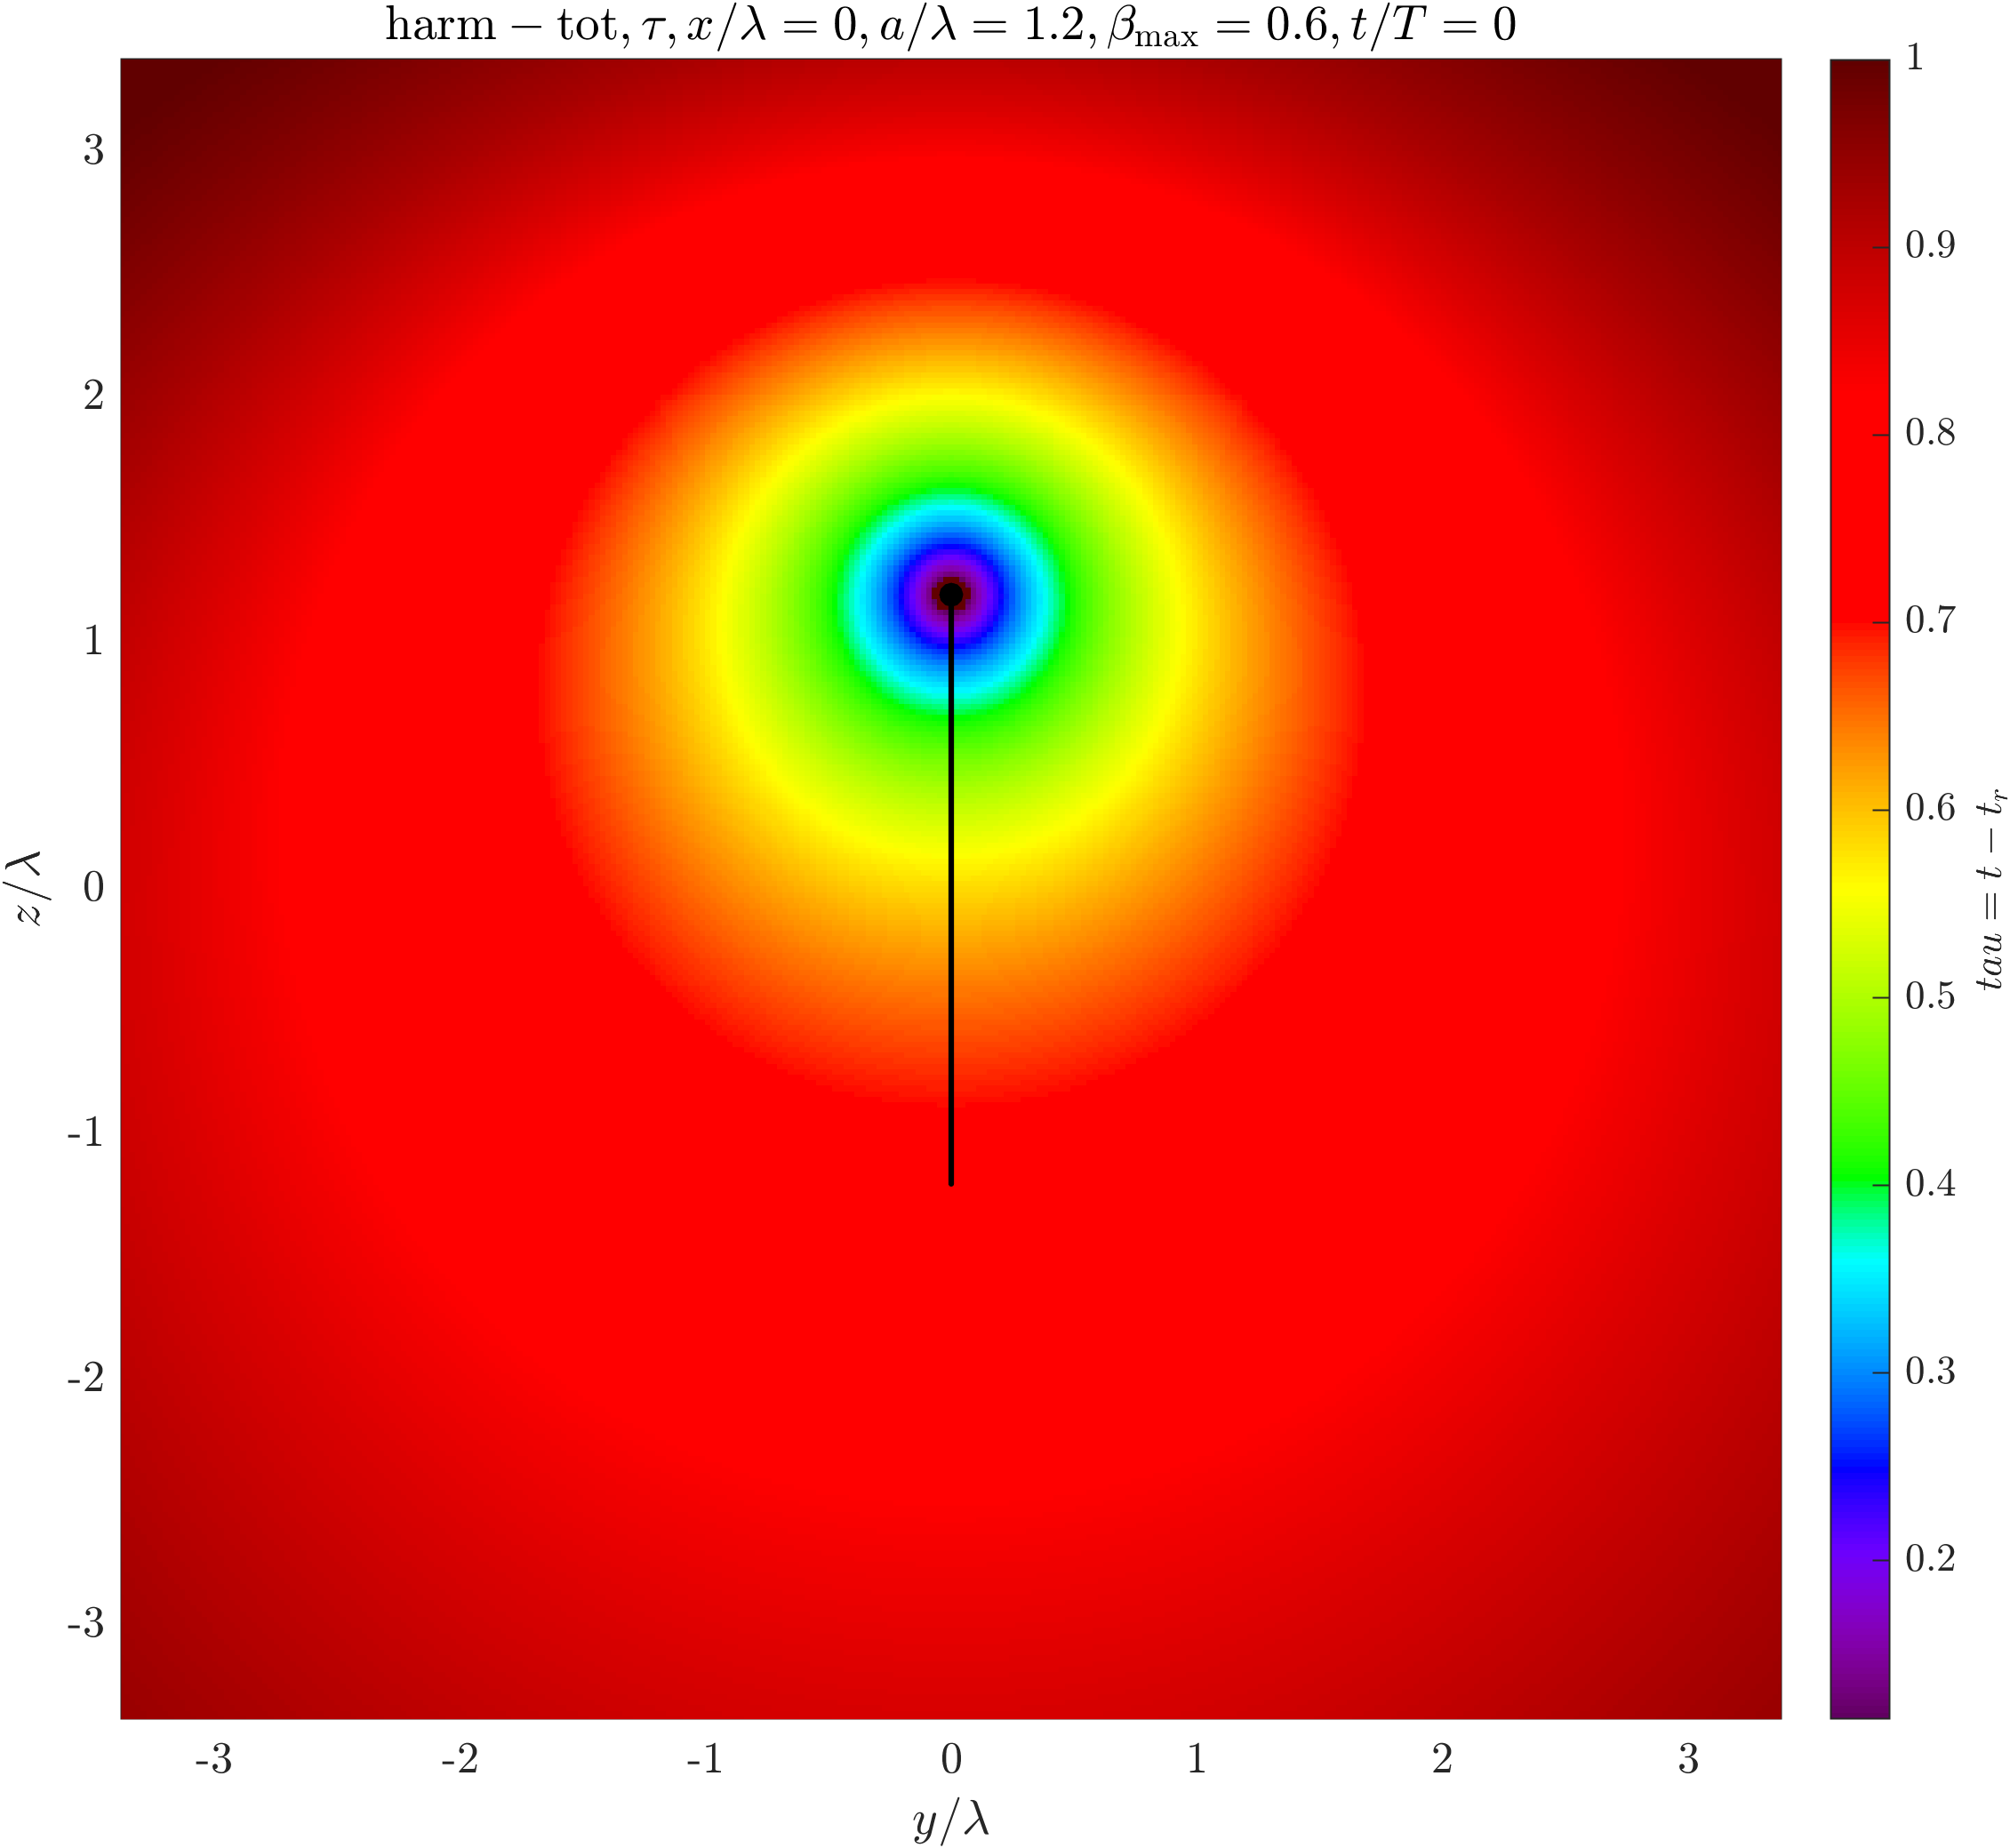
\includegraphics[width=\textwidth]{radiation_fig/harmonic_motion_tau_yz_beta_0_6_eta_0.png}
		\caption{\(\tau|_{yz}\) (\(\beta=0.6\), \(\eta=0\))}
		\label{点电荷简谐运动辐射场示意图-tau|_yz(beta=0.6,eta=0)}
	\end{subfigure}
	\hfill
	\begin{subfigure}[b]{0.23\textwidth}
		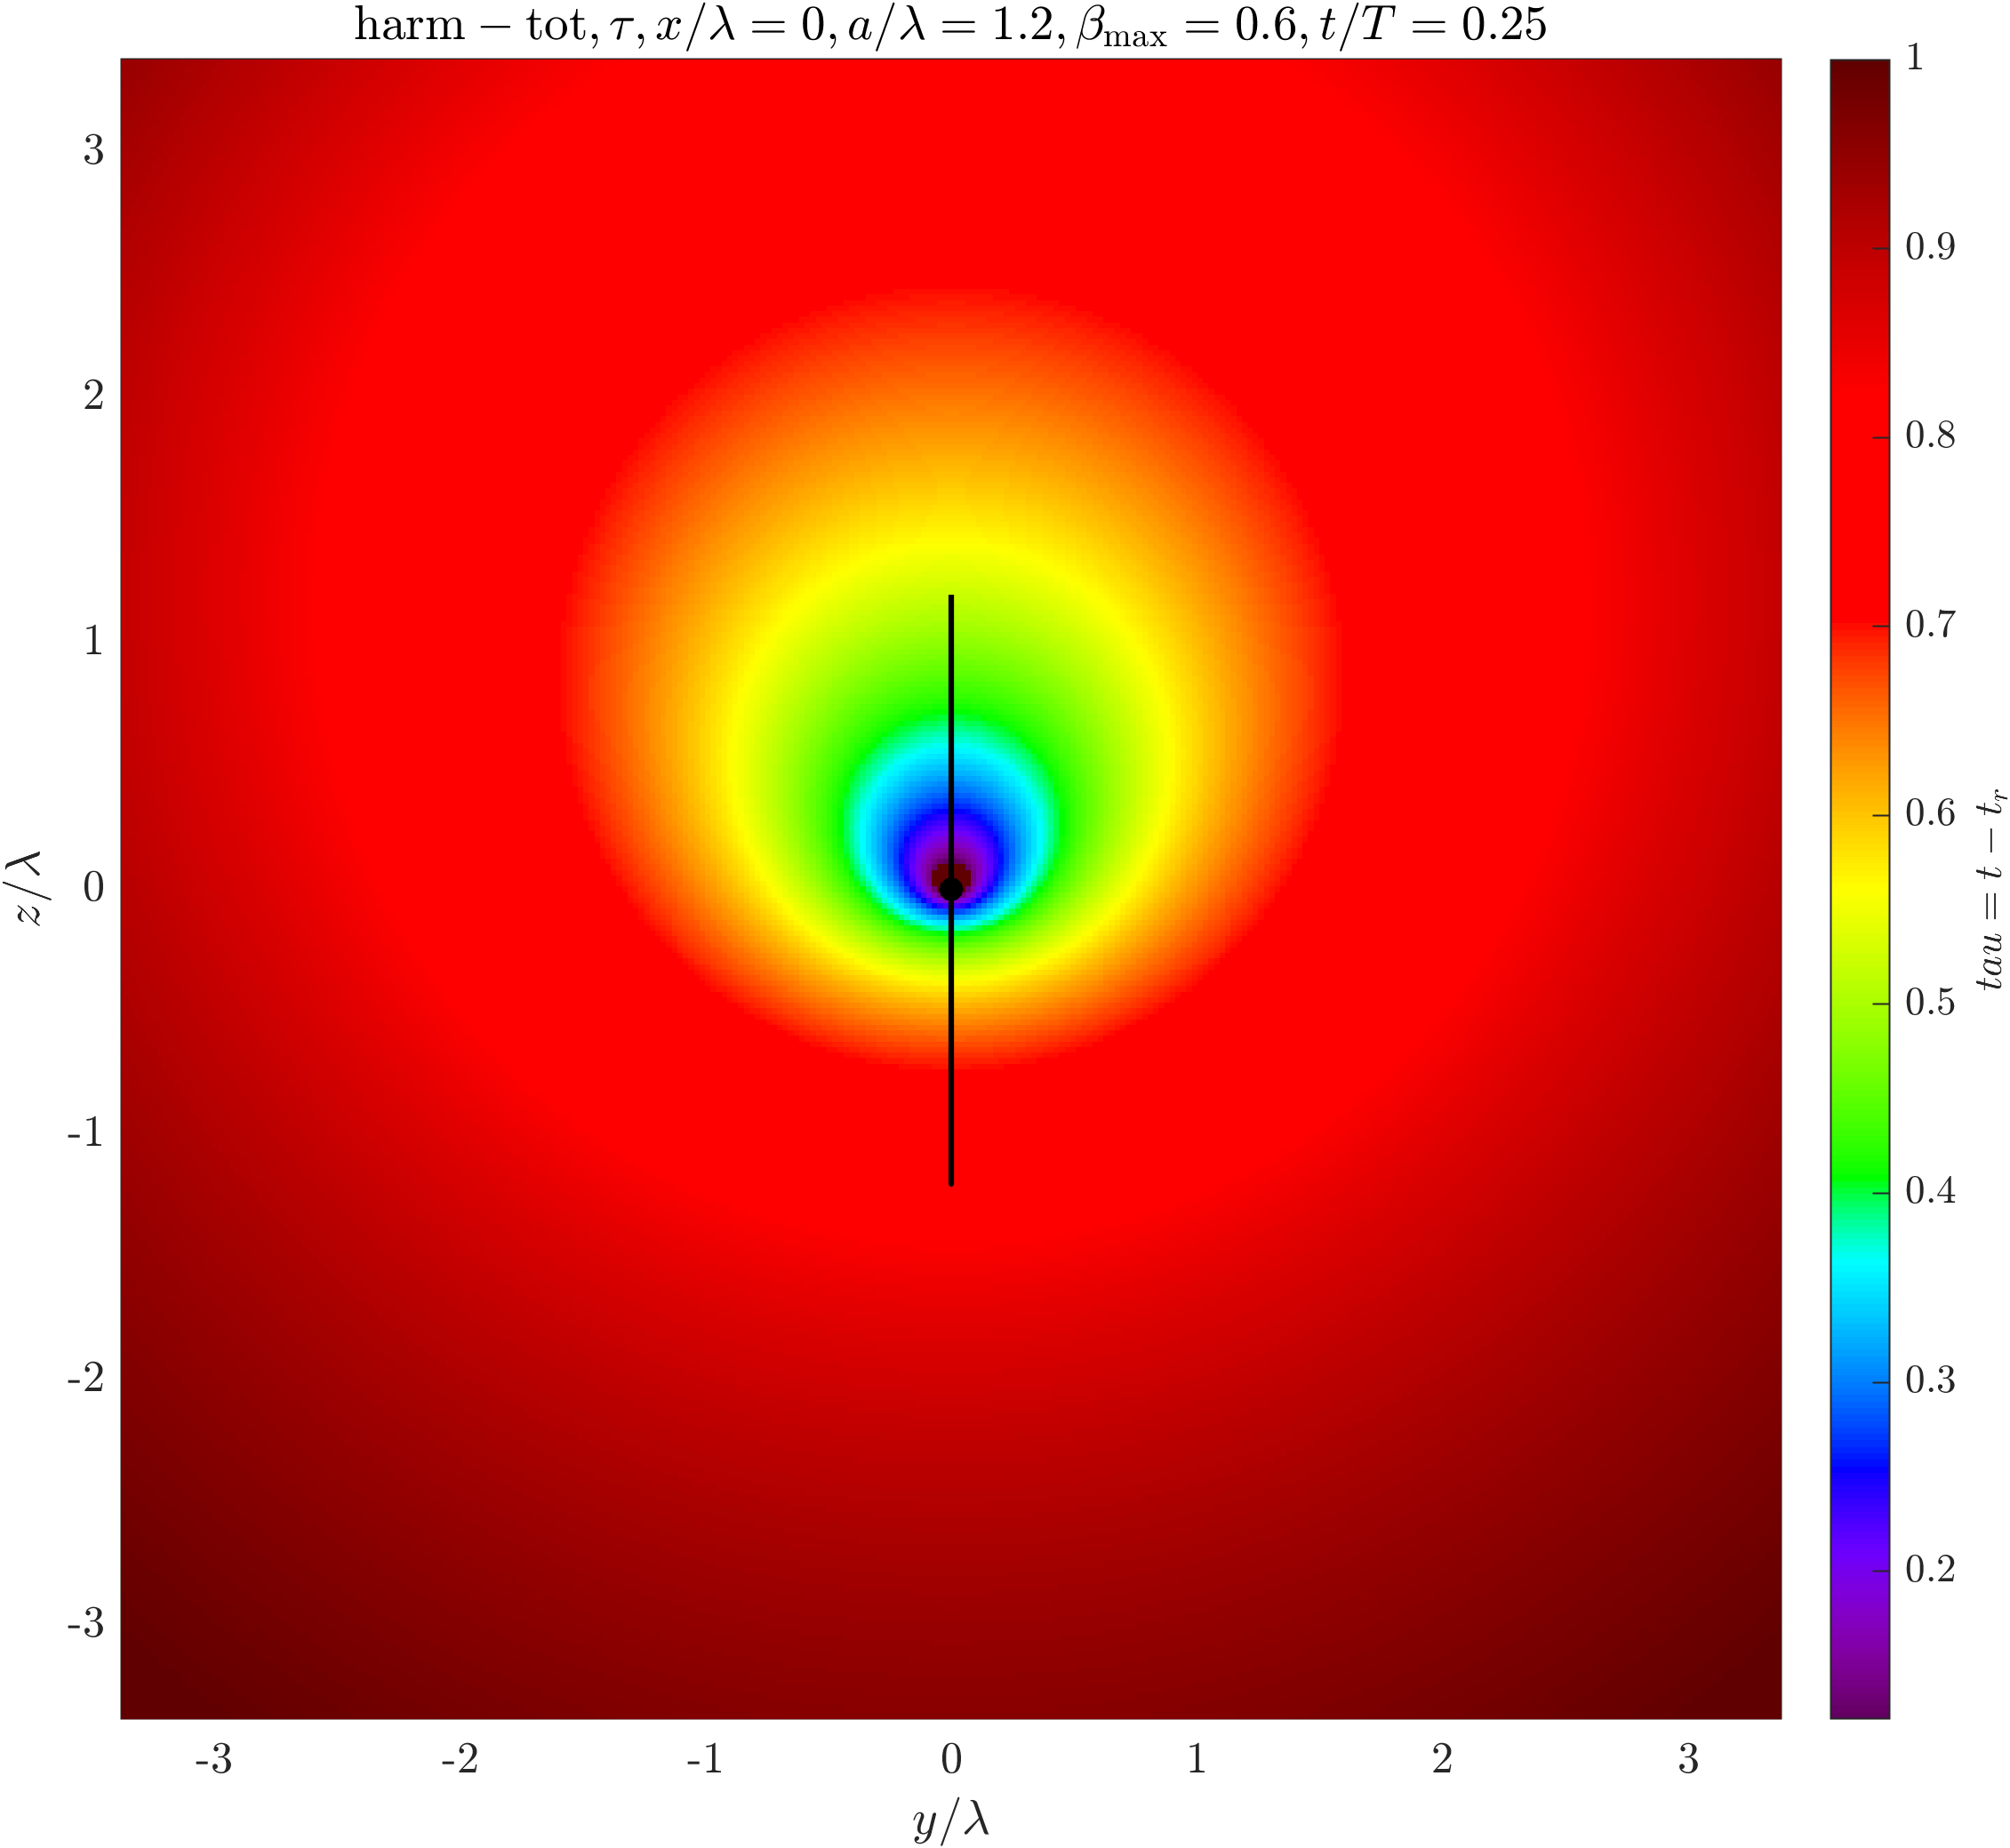
\includegraphics[width=\textwidth]{radiation_fig/harmonic_motion_tau_yz_beta_0_6_eta_0_25.png}
		\caption{\(\tau|_{yz}\) (\(\beta=0.6\), \(\eta=0.25\))}
		\label{点电荷简谐运动辐射场示意图-tau|_yz(beta=0.6,eta=0.25)}
	\end{subfigure}
	\hfill
	\begin{subfigure}[b]{0.23\textwidth}
		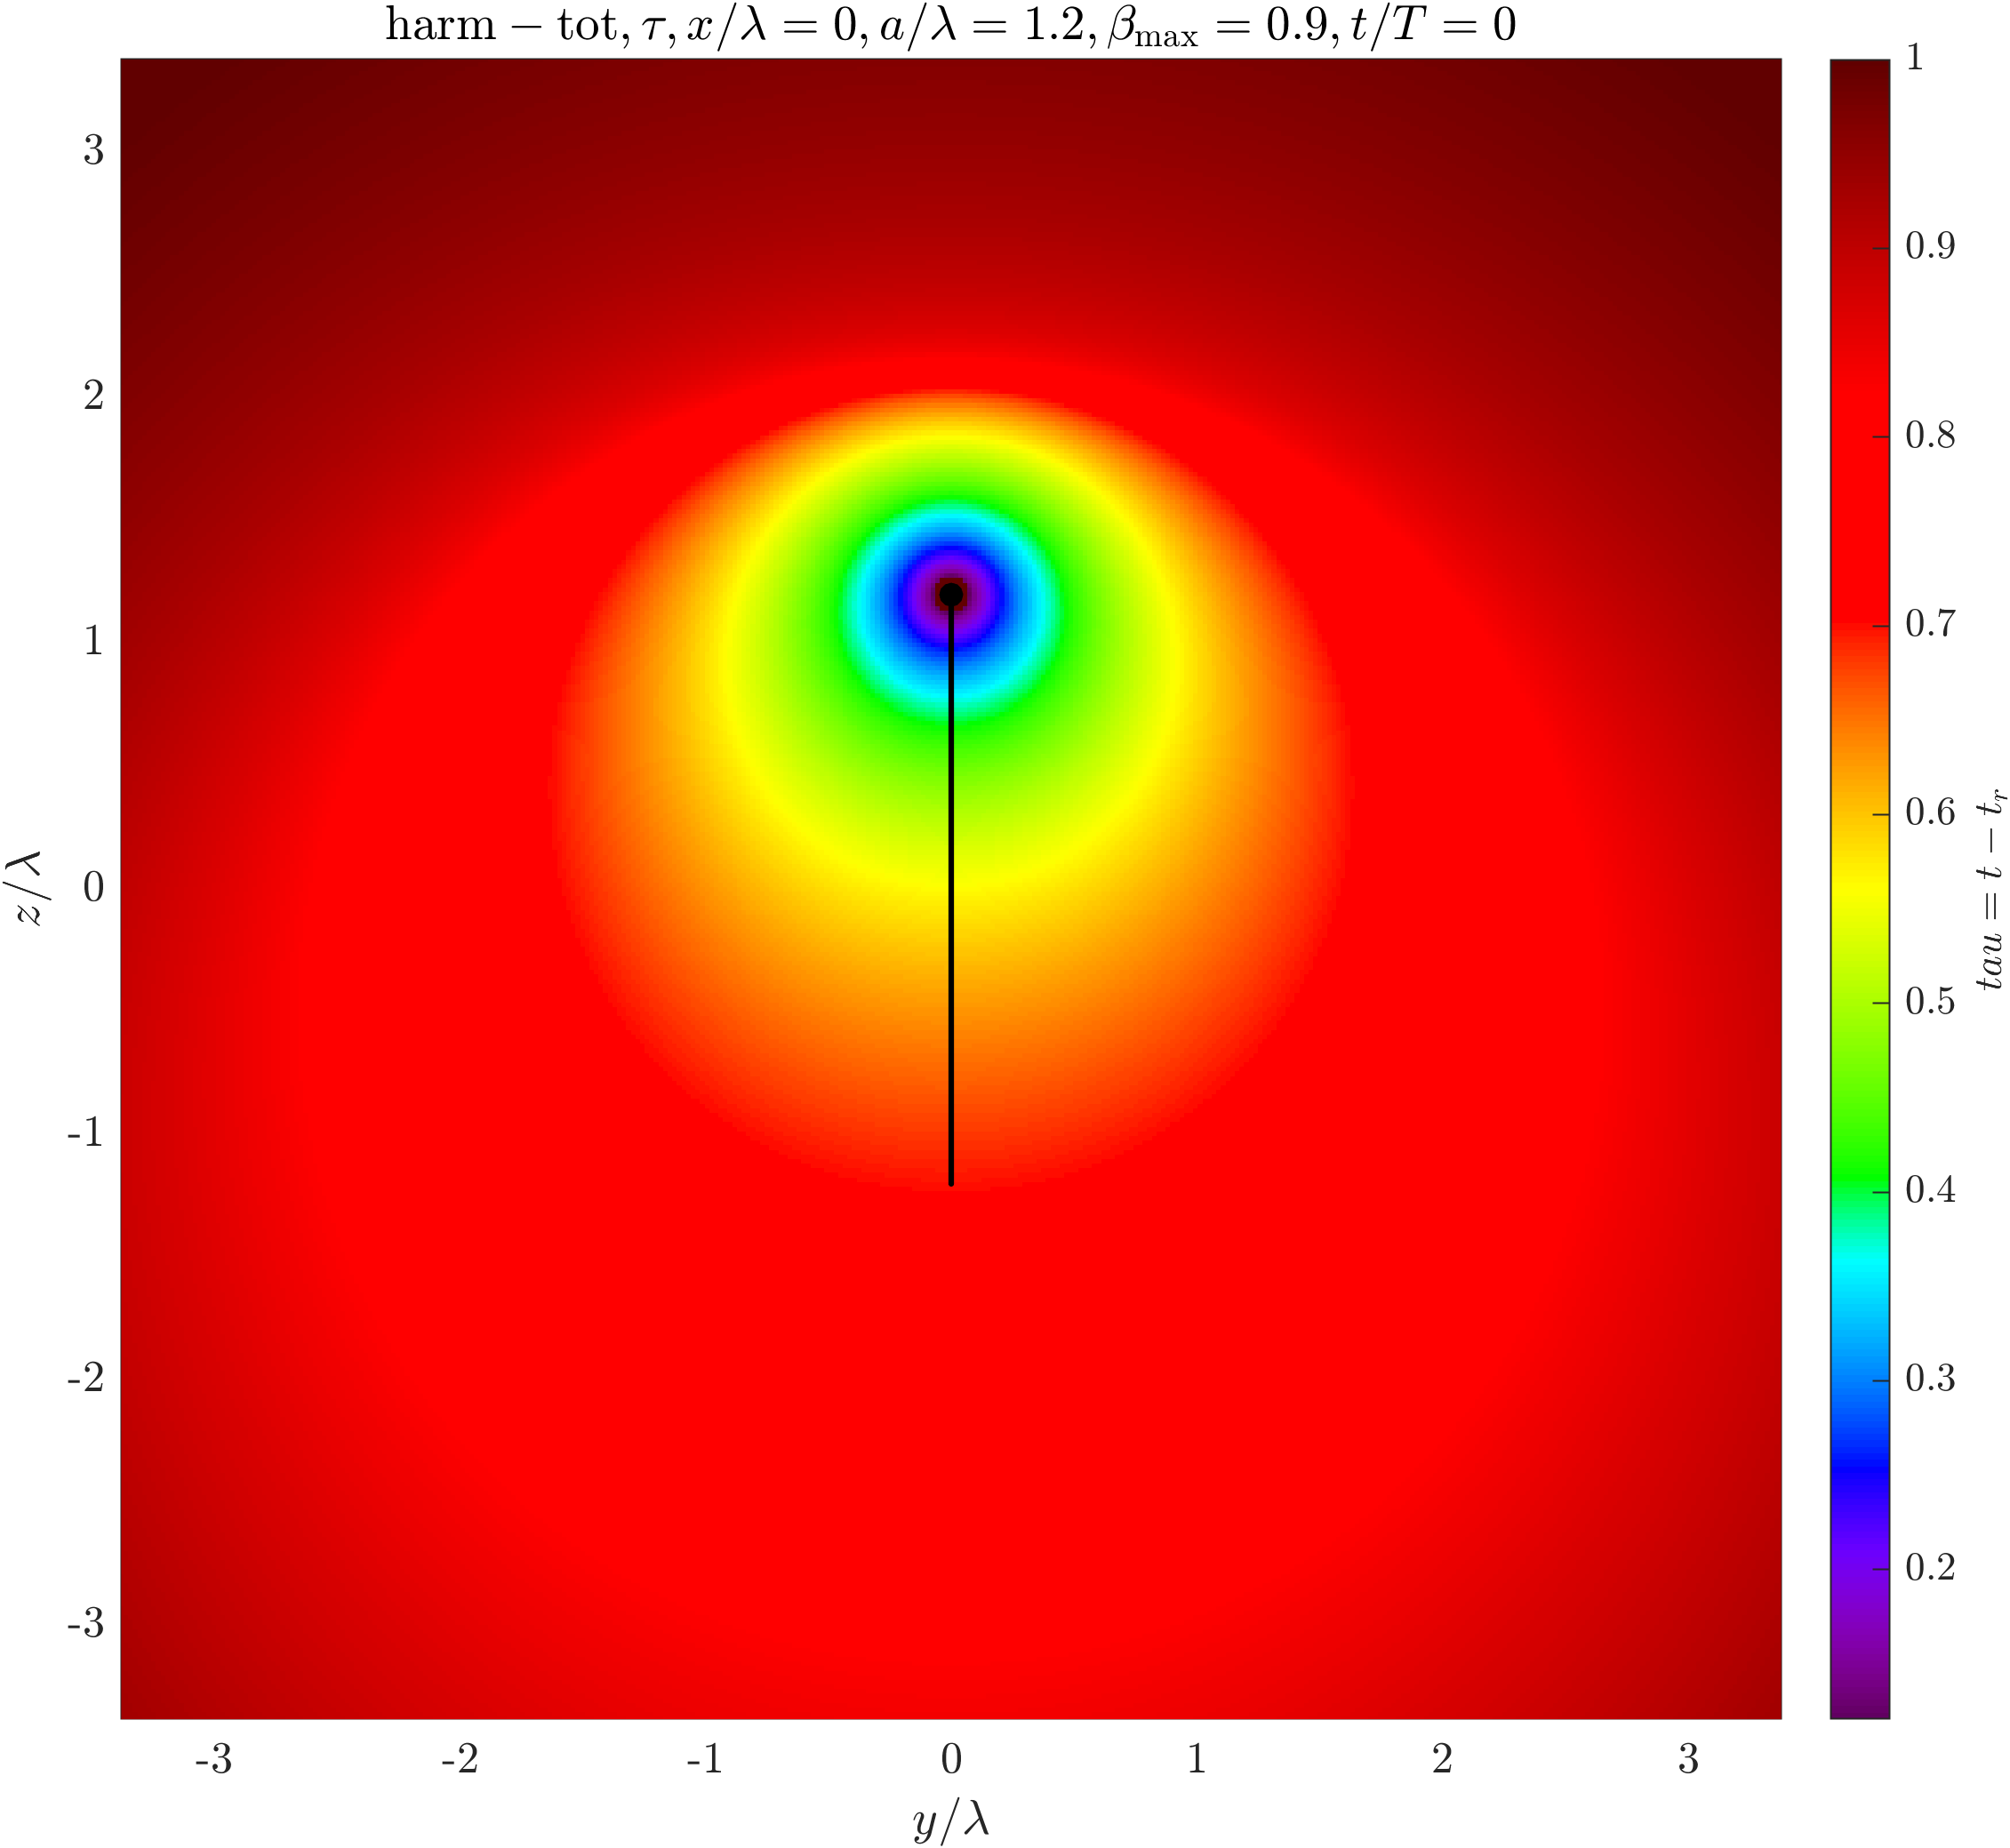
\includegraphics[width=\textwidth]{radiation_fig/harmonic_motion_tau_yz_beta_0_9_eta_0.png}
		\caption{\(\tau|_{yz}\) (\(\beta=0.9\), \(\eta=0\))}
		\label{点电荷简谐运动辐射场示意图-tau|_yz(beta=0.9,eta=0)}
	\end{subfigure}
	\hfill
	\begin{subfigure}[b]{0.23\textwidth}
		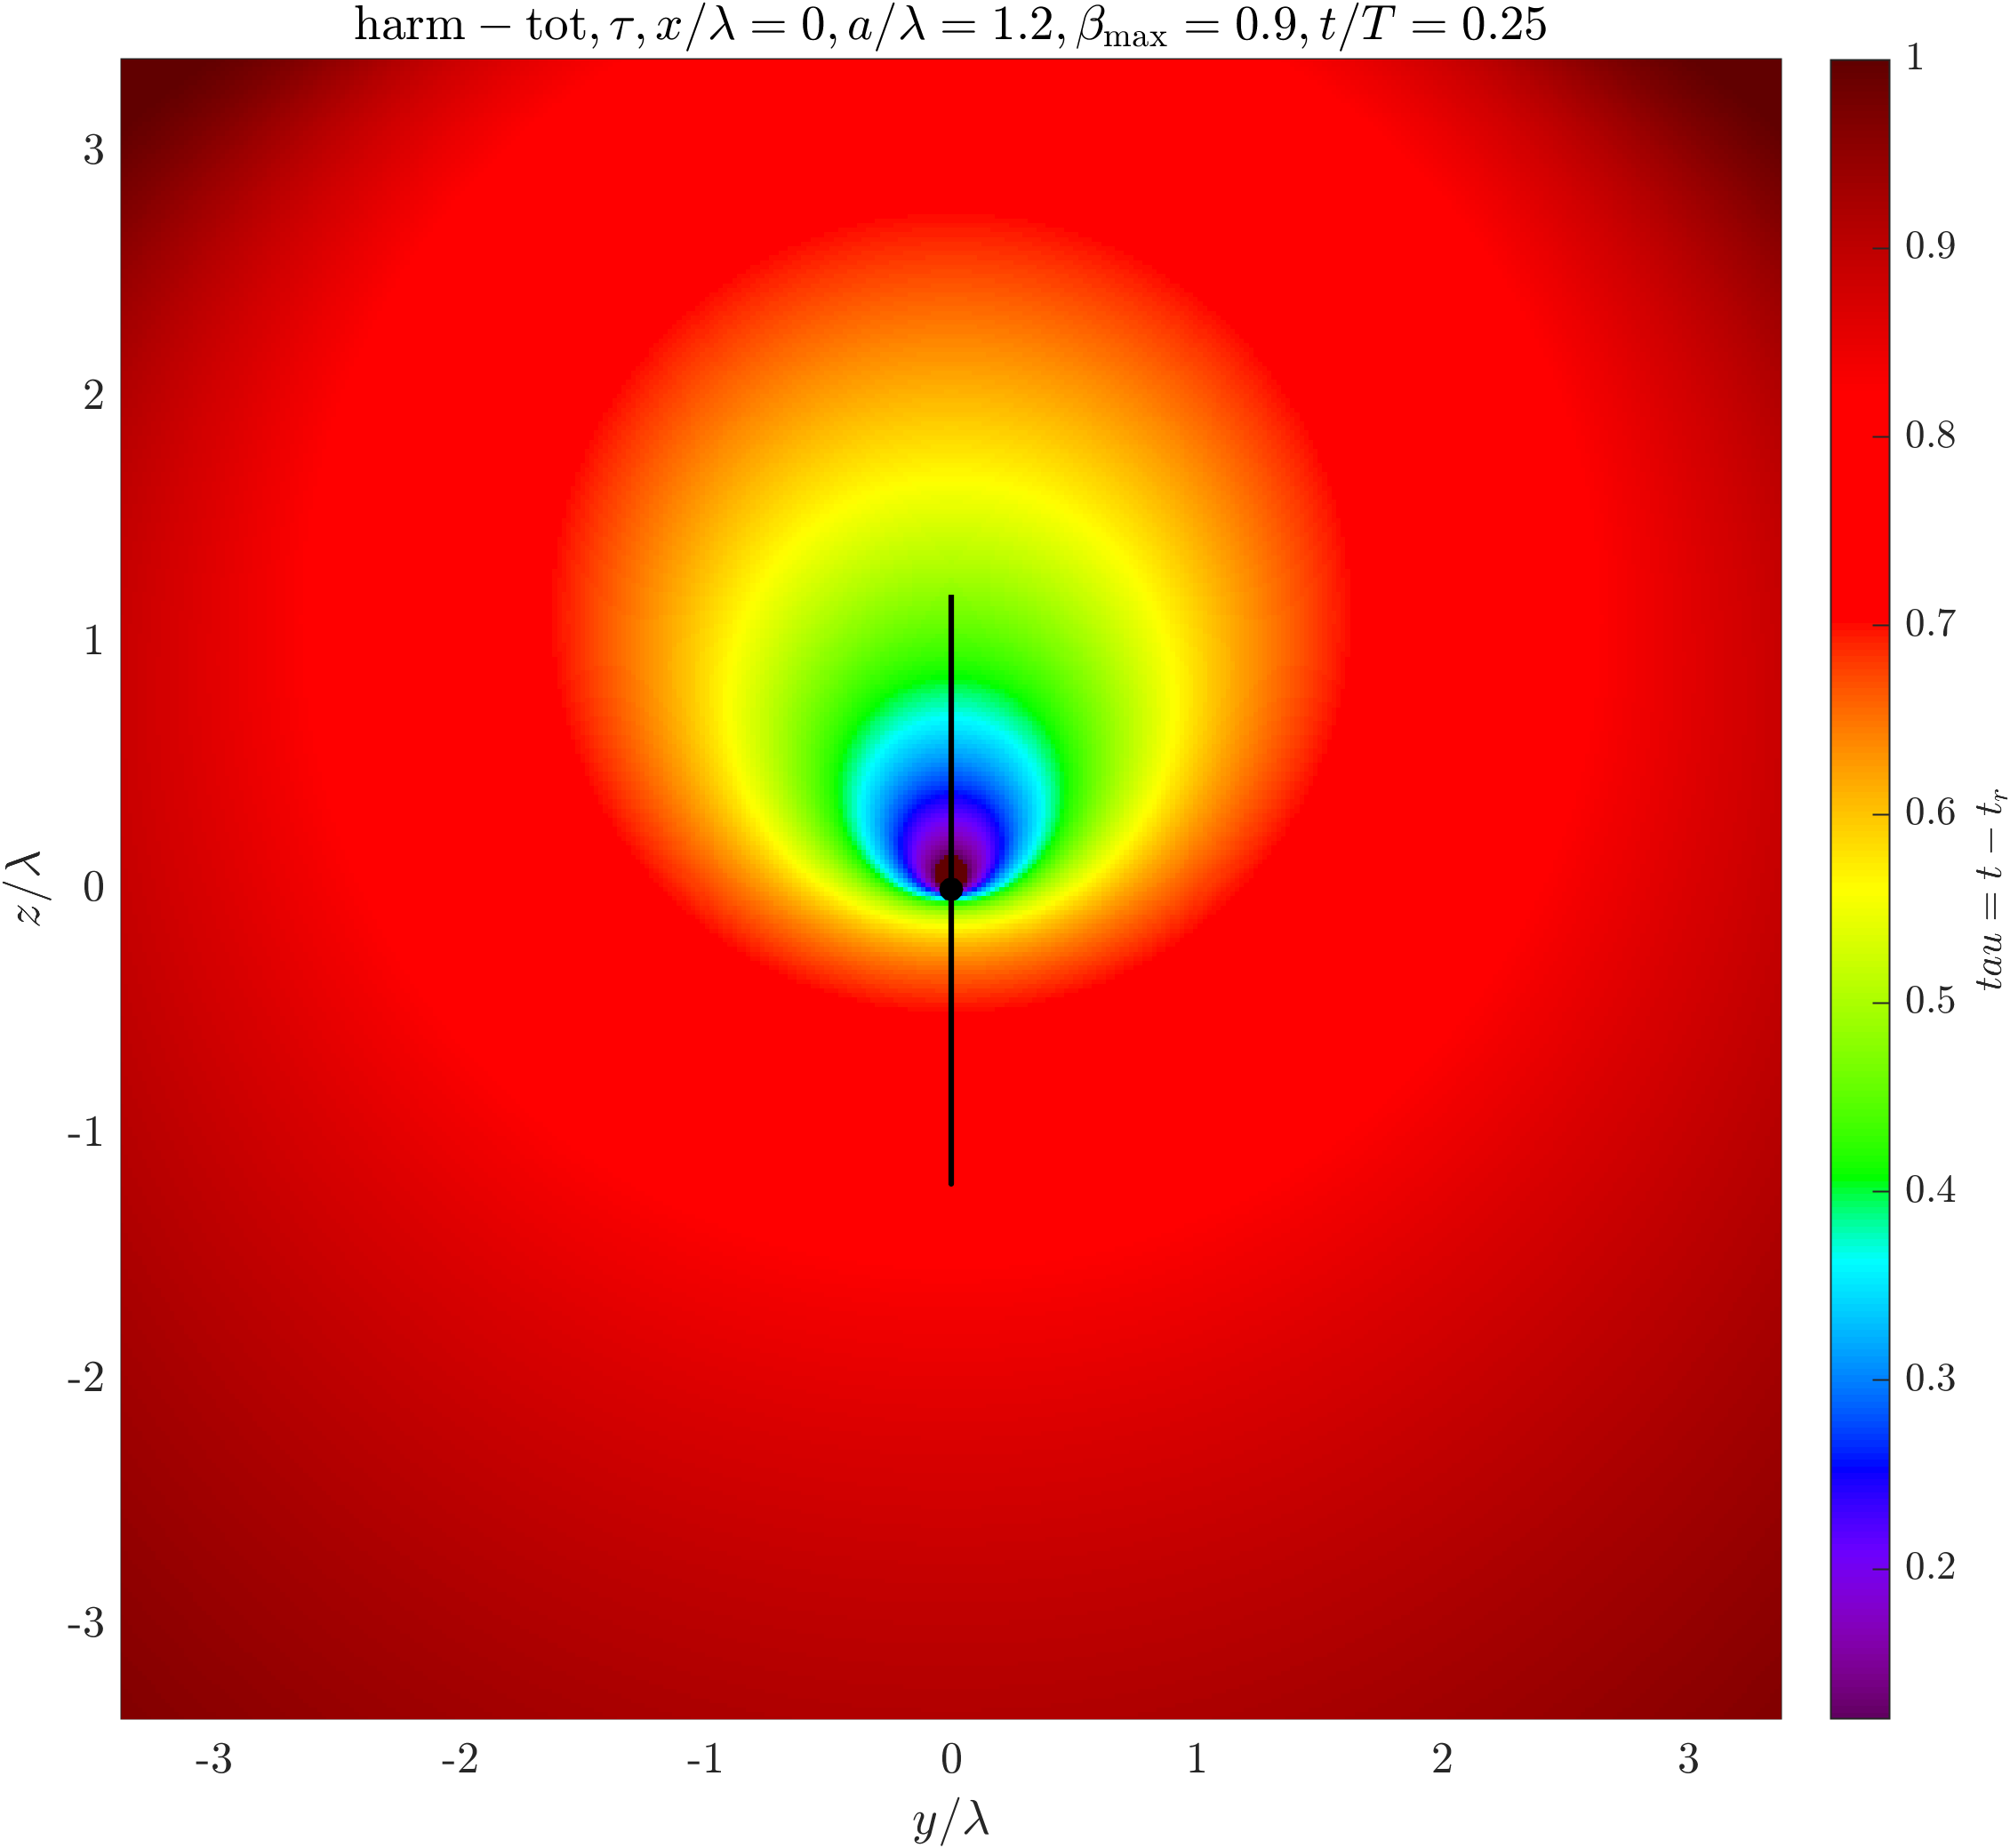
\includegraphics[width=\textwidth]{radiation_fig/harmonic_motion_tau_yz_beta_0_9_eta_0_25.png}
		\caption{\(\tau|_{yz}\) (\(\beta=0.9\), \(\eta=0.25\))}
		\label{点电荷简谐运动辐射场示意图-tau|_yz(beta=0.9,eta=0.25)}
	\end{subfigure}

	\caption{点电荷简谐运动辐射场示意图}
	\label{点电荷简谐运动辐射场示意图}
\end{figure}
